\documentclass{beamer}

\usetheme{Montpellier}
\usecolortheme{seagull}
% Rather be using my own color
\definecolor{LightGrey}{rgb}{0.84,0.83,0.83}
\definecolor{LightYell}{rgb}{0.90,0.83,0.70}
\definecolor{StroYell}{rgb}{0.95,0.88,0.72}
\definecolor{myem}{rgb}{0.797,0.598,0.598}
\definecolor{lightred}{rgb}{0.75,0.033,0}
\definecolor{shadecolor1}{rgb}{0.90,0.83,0.70}

\setbeamercolor{structure}{fg=myem!120}
%\setbeamercolor{example}{bg=LightYell,fg=StroYell}
\setbeamercolor{alerted text}{fg=lightred}
\setbeamertemplate{blocks}[rounded][shadow=true]
\setbeamertemplate{footline}[page number]

\usefonttheme[onlymath]{serif}
\renewcommand{\thefootnote}{\fnsymbol{footnote}}
\useinnertheme{rounded}

% Compatibility with zbook
\usepackage{ifthen}
\newboolean{sv_used}
\setboolean{sv_used}{false}
%%%%%%%%%%%%%%%%%%
% Text conventions
\newcommand{\etal}{et al.}
\newcommand{\wrt}{with respect to}
\newcommand{\rhs}{right-hand side}
\newcommand{\lhs}{left-hand side}
\newcommand{\iid}{\stackrel{i.i.d.}{\sim}}
\newcommand{\as}{a.s.}
\newcommand{\mae}{a.e.}
\newcommand{\ie}{i.e.}
\newcommand{\eg}{e.g.}
\newcommand{\cf}{cf.}
\newcommand{\pdf}{probability density function}
\newcommand{\eqsp}{\;}

%%%%%%%%%%%%%%%%%%%
% General math defs
\newcommand{\rset}{\ensuremath{\mathbb{R}}}
\newcommand{\nset}{\ensuremath{\mathbb{N}}}
\newcommand{\zset}{\ensuremath{\mathbb{Z}}}
\newcommand{\lone}{\ensuremath{L^1}}
\newcommand{\ltwo}{\ensuremath{L^2}}
\newcommand{\scalprod}[2]{\ensuremath{\langle #1, #2 \rangle}}
\newcommand{\linspan}{\ensuremath{\operatorname{span}}}
\newcommand{\proj}[2]{\ensuremath{\operatorname{proj}({#1}|#2)}}
\newcommand{\1}{\ensuremath{\mathbbm{1}}}
\newcommand{\argmin}{\ensuremath{\operatorname{arg\,min}}}
\newcommand{\argmax}{\ensuremath{\operatorname{arg\,max}}}
\newcommand{\eqdef}{\ensuremath{\stackrel{\mathrm{def}}{=}}}
\newcommand{\card}[1]{\ensuremath{|#1|}}
\newcommand{\tvnorm}[1]{\ensuremath{\left\|#1\right\|_{\mathrm{TV}}}}
\newcommand{\tvnormsmall}[1]{\ensuremath{\|#1\|_{\mathrm{TV}}}}
\newcommand{\rmd}{\ensuremath{\mathrm{d}}}
\newcommand{\rmi}{\ensuremath{\mathrm{i}}}
\newcommand{\rme}{\ensuremath{\mathrm{e}}}
\newcommand{\mcb}[1]{\ensuremath{\mathcal{F}_{\mathrm{b}}\left(#1\right)}}
\newcommand{\mcp}[1]{\ensuremath{\mathcal{F}_{+}\left(#1\right)}}
\newcommand{\supnorm}[1]{\ensuremath{\left\|#1\right\|_{\infty}}}

%%%%%%%%%%%%%%%%%%%
% If svmult is not available replace with equivalents using the amsthm
% environment
\usepackage{amsthm}
\newtheorem{thm}{Theorem}
\newtheorem{prop}[thm]{Proposition}
\newtheorem{cor}[thm]{Corollary}
\newtheorem{lem}[thm]{Lemma}
%\newtheorem{definition}[thm]{Definition}
\newtheorem{assum}[thm]{Assumption}
\theoremstyle{definition}\newtheorem{rem}[thm]{Remark}
\theoremstyle{definition}\newtheorem{ex}[thm]{Example}
\theoremstyle{definition}\newtheorem{algo}[thm]{Algorithm}

\usepackage{natbib}
\usepackage{amsmath}
\usepackage{amsfonts}
\usepackage{amssymb}
\usepackage{bbm}
\usepackage{mathrsfs}

\usepackage{color}
\usepackage{ifthen}
\usepackage{enumerate}
\usepackage{makeidx}
\usepackage{multicol}
\usepackage[bottom]{footmisc}
\usepackage{boxedminipage}
\usepackage{stmaryrd}
\usepackage{changebar}
\usepackage{framed}
\usepackage{colordvi}
\usepackage{fancyhdr,scrtime}

\usepackage{graphicx,picins,stmaryrd}


\input{cmacros}
\input colordvi

% Compatibility with seminar
\newenvironment{slide}%
 {\begin{frame}}%
 {\end{frame}}
\newcommand{\slidetitle}{\frametitle}

\usepackage{graphicx,picins,stmaryrd,lastpage}

\usepackage{verbatim}

%\def\path{/home/xian/Books/MCSM2/figures}
\newcommand{\btheta}{\mbox{\boldmath{$\theta$}}}
\newcommand{\covrm}{\mathrm{cov}}
\newcommand{\emfarite}[1]{\rightline{\RedViolet{\sf [#1]}}\hglue 3.2truecm}

\def\baro{\medskip \hfill \hrule height.5pt \vskip .3truecm}
\def\barba{\vskip -.3truecm\hfill \hrule height.5pt \vskip .8truecm}

\newcommand\debut{\begin{example}}
\newcommand\fin{\end{example}}

% Lines in tables
\newcommand\laligne{
\noalign{\vskip .3em}
\noalign{\hrule}
\noalign{\vskip .3em}
}
\newcommand\labelenumi{\theenumi}

% les k_n'ries a mimi!
\newcommand{\vs}{\vspace{0.5cm}}
\newcommand{\tee}{\mathrm{T}}
\newcommand{\bx}{\mathbf{x}}
\newcommand{\by}{\mathbf{y}}
\newcommand{\bX}{\mathbf{X}}
\newcommand\bp{\mathbf{p}}
\newcommand\bz{{\bf z}}
% & celles a j'rom
\newcommand\sos{{{\phi}_t(r)}}
\newcommand\ps{{p_t(r)}}
\newcommand\qs{{q_t(r,s)}}
\newcommand\xs{x_{(i,t)}}
\newcommand\zs{z_{(i,t)}}
\newcommand\zsa{z_{(i,t+1)}}
% & les miennes
\newcommand\GoM{\mathfrak{M}}
\newcommand\GoK{\mathfrak{K}}

%Warning, refs only
\includeonly{}

%%%%%%%%%%%%%%%%%%%%%%%%%%%%%%%%%%%%%%%%%%%%%%%%%%%%%%%%%%%%%%%%%%%%%
\title{Bayesian Core:\\A Practical Approach to
Computational Bayesian Statistics}
\author{Jean-Michel Marin \&\ Christian P. Robert}
\date{QUT, Brisbane, August 4--8 2008}

\begin{document}
%%%%%%%%%%%%%%%%%%%%%%%%%%%%%%%%%%%%%%%%%%%%%%%%%%%%%%%%%%%%%%%%%%%%%%%%%%%%%%%
\begin{slide}
  \titlepage
  \centerline{\includegraphics[height=5truecm]{BCS.ps}}
\end{slide}

%%%%%%%%%%%%%%%%%%%%%%%%%%%%%%%%%%%%%%%%%%%%%%%%%%%%%%%%%%%%%%%%%%%%%%%%%%%%%%%
\begin{slide}
  \slidetitle{Outline}
  {\small
  \tableofcontents[subsectionstyle=hide]
  }
\end{slide}

%%%%%%%%%%%%%%%%%%%%%%%%%%%%%%%%%%%%%%%%%%%%%%%%%%%%%%%%%%%%%%%%%%%%%%%%%%%%%%%
\section{The normal model}
\begin{slide}\slidetitle{The normal model}
\tableofcontents[sectionstyle=show/hide,subsectionstyle=show/shaded/hide]

\end{slide}
\subsection{Normal problems}\begin{slide}\slidetitle{Normal model}
Sample
$$
x_1,\ldots,x_n
$$
from a normal $\mathcal{N}(\mu,\sigma^2)$ distribution

\centerline{\includegraphics[height=\textwidth,width=5truecm,angle=270]{figures/normalsample.ps}}

\end{slide}\begin{slide}
\slidetitle{Inference on $(\mu,\sigma)$ based on this sample}

\begin{itemize}
\item Estimation of \RedOrange{[transforms of]} $(\mu,\sigma)$ 
\pause
\item Confidence region \RedOrange{[interval]} on $(\mu,\sigma)$
\pause
\item Test on $(\mu,\sigma)$ and comparison with other samples
\end{itemize}

\end{slide}
\begin{slide}\slidetitle{Datasets}
\begin{block}{\BurntOrange{\bfseries {Larcenies {\sf =normaldata}}}}
\begin{columns}
\column{.45\textwidth}
Relative changes in reported
larcenies between 1991 and 1995 (relative to 1991)
for the $90$ most populous US counties {\em (Source: FBI)}
\column{.45\textwidth}
%\only<1>{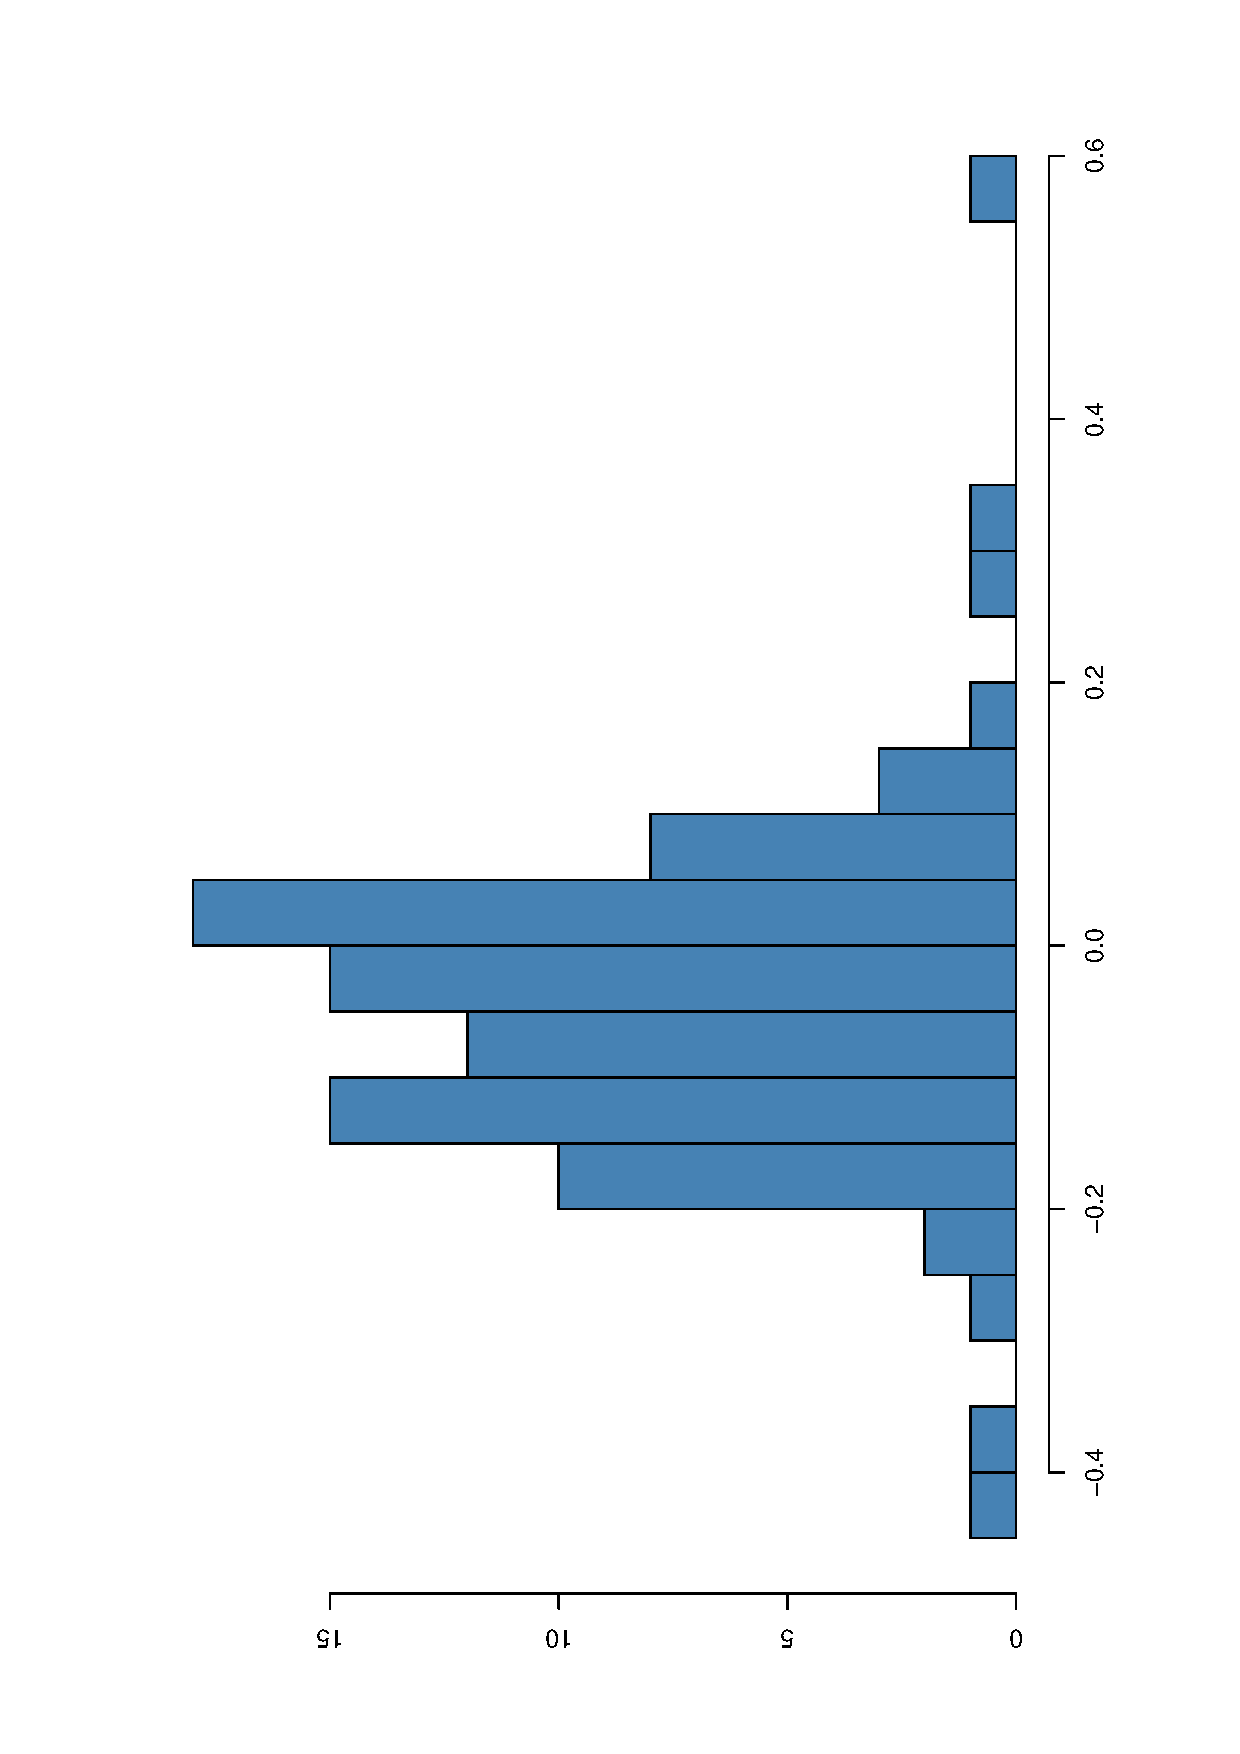
\includegraphics[height=5truecm,width=5truecm,angle=270]{figures/normdata}}
%\only<2>{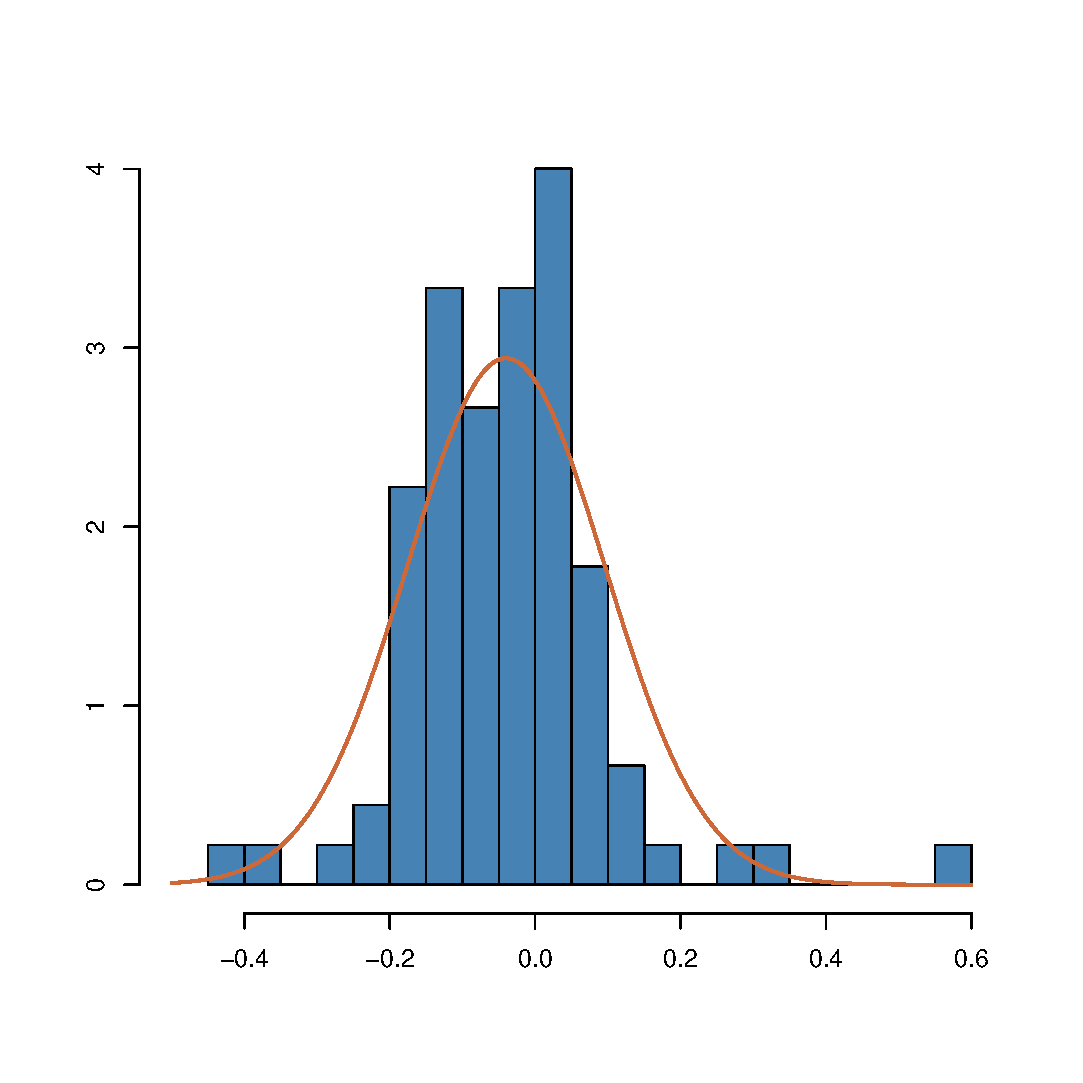
\includegraphics[height=5truecm,width=5.3truecm]{figures/normdataplus}}
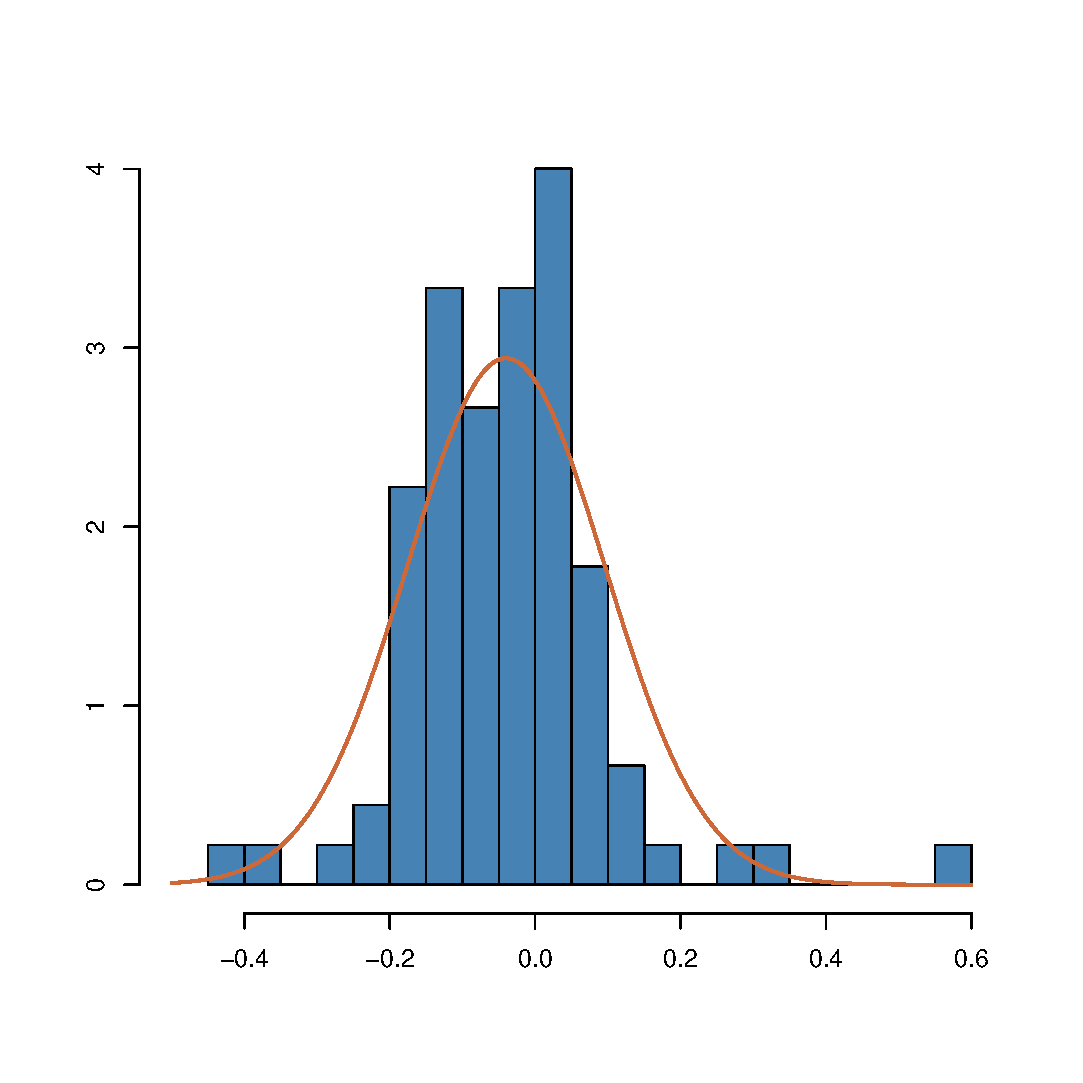
\includegraphics[height=5truecm,width=5.3truecm]{figures/normdataplus}
\end{columns}
\end{block}
\end{slide}
\begin{slide}
\begin{block}{\BurntOrange{\bfseries {Cosmological background {\sf =CMBdata}}}}
\begin{columns}
\column{.5\textwidth}
Spectral representation of the ``cosmological microwave background" (CMB),
i.e.~ electromagnetic radiation from photons back to $300,000$ years
after the Big Bang, expressed as difference in apparent temperature from the mean
temperature
\column{.45\textwidth}
\only<1>{\includegraphics[height=5truecm,width=5truecm,angle=270]{figures/CMBcol}}

\end{columns}
\end{block}
\end{slide}
\begin{slide}
\begin{block}{\BurntOrange{\bfseries {Cosmological background {\sf =CMBdata}}}}
Normal estimation
\only<1>{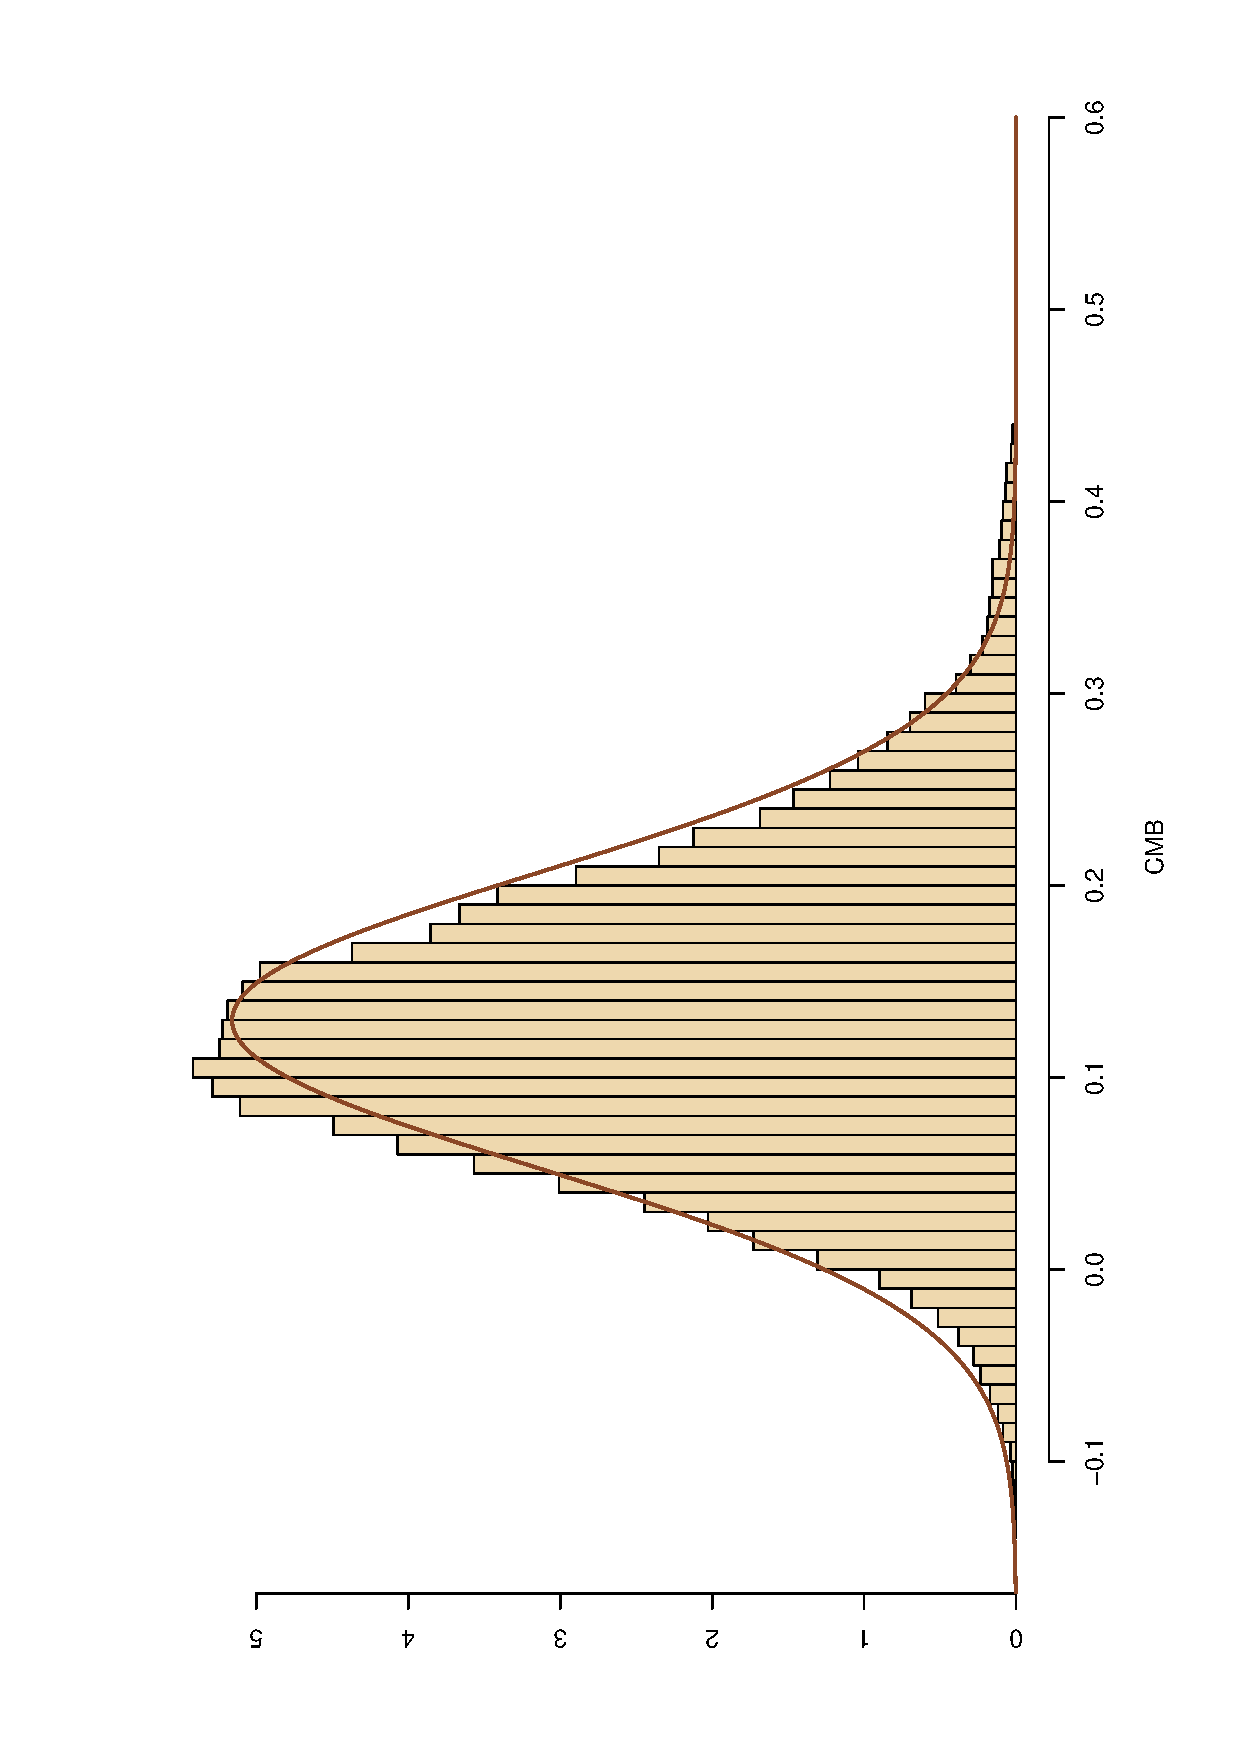
\includegraphics[height=5truecm,width=5truecm,angle=270]{figures/CMBnor}}
\end{block}
\end{slide}
\begin{slide}
\begin{block}{\BurntOrange{\bfseries {Cosmological background {\sf =CMBdata}}}}
Normal estimation
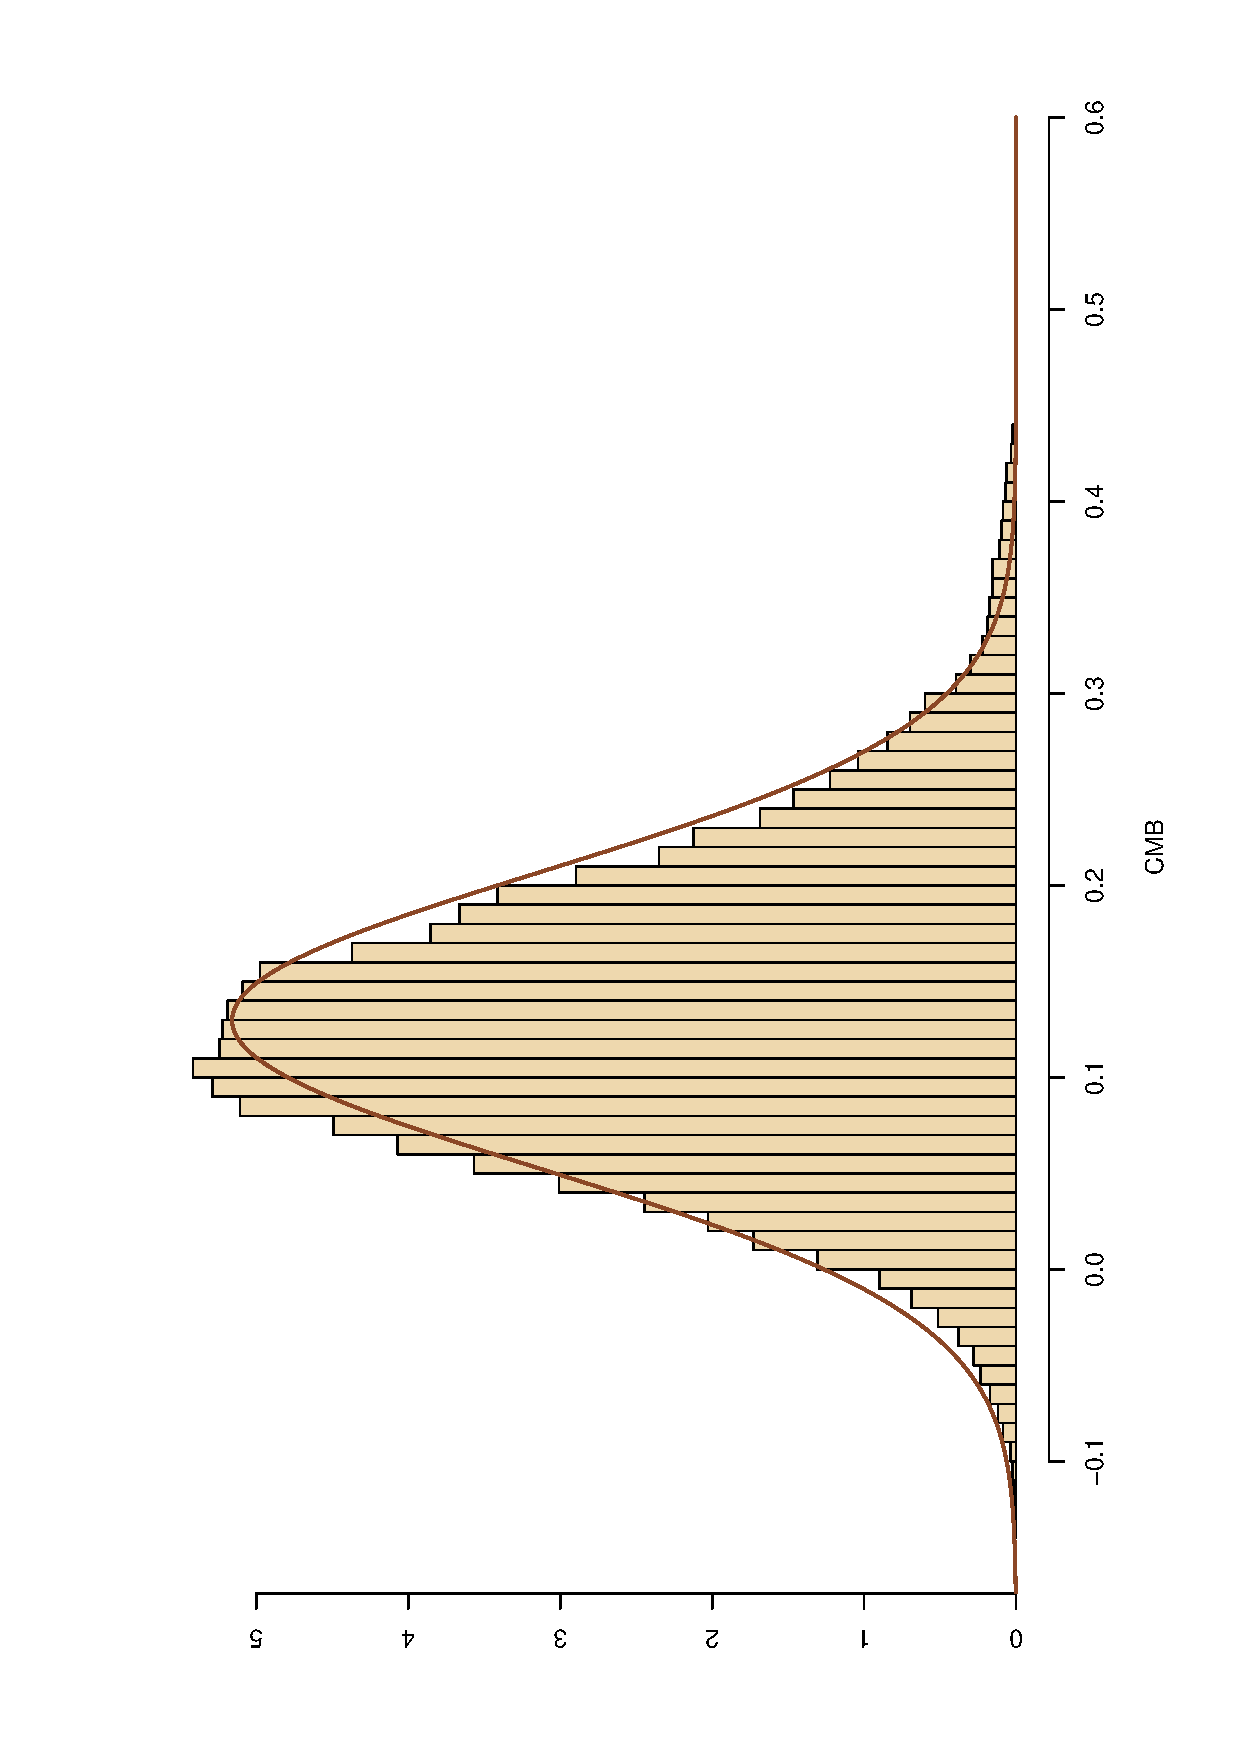
\includegraphics[height=5truecm,width=5truecm,angle=270]{figures/CMBnor}
\end{block}
\end{slide}

\subsection{The Bayesian toolbox}\begin{slide}\slidetitle{The Bayesian toolbox}

\centerline{\BurntOrange{\fbox{\bf Bayes theorem = Inversion of probabilities}}}

\bigskip
\pause
If $A$ and $E$ are events such that $P(E)\ne 0$, $P(A|E)$ and $P(E|A)$ are related by
{\Brown{
\begin{eqnarray*}
P(A|E) &=& {P(E|A) P(A) \over P(E|A) P(A) + P(E|A^c) P(A^c)}\\
&=& {P(E|A) P(A) \over P(E)} 
\end{eqnarray*}
}}

\end{slide}
\begin{slide}
\slidetitle{\Blue{\sf Who's Bayes?}}

\begin{block}{\BrickRed{{\bf Reverend Thomas Bayes (ca. 1702--1761)}}}
\begin{columns}\column{.5\textwidth}
Presbyterian minister in Tunbridge Wells (Kent) from 1731, son of Joshua Bayes, nonconformist minister.
Election to the {\em Royal Society} based on a tract of 1736 where he defended the views
and philosophy of Newton.

\column{.4\textwidth}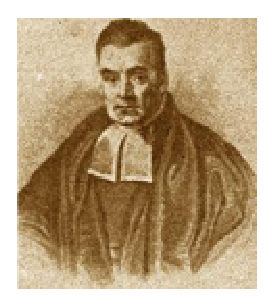
\includegraphics[height=4truecm]{figures/TBayes}
\end{columns}

\medskip
\pause
Sole probability paper, {\em ``Essay Towards Solving a Problem in the Doctrine of Chances"},
published posthumously in 1763 by Pierce
and containing the seeds of {\em Bayes' Theorem}.%Philosophical Transactions of the Royal Society of London.
\end{block}

\end{slide}
\begin{slide}
\slidetitle{New perspective}
\begin{itemize}
\item {\it Uncertainty} on the parameters $\theta$ of a model 
modeled through a {\it probability} distribution $\pi$ on $\Theta$, 
called {\it prior distribution}

\pause
\item {\it Inference} based on the distribution of $\theta$ conditional 
on $x$, $\pi(\theta|x)$, called {\it posterior distribution}
{\Brown{
\[
\pi(\theta|x) = {f(x|\theta) \pi(\theta) \over \int f(x|\theta) 
     \pi(\theta) \,d\theta}\ .
\]
}}
\end{itemize}

\end{slide}\begin{slide}
\slidetitle{Bayesian model}

A Bayesian statistical model is made of 
\begin{enumerate}
\item a likelihood \[{\Red{ f(x|\theta), }}\]
\pause and of 
\item a prior distribution on the parameters, \[{\Red{ \pi(\theta)\,. }}\]
\end{enumerate}

\end{slide}\begin{slide}
\slidetitle{Justifications}

\begin{itemize}
\item Semantic drift from unknown $\theta$ to random $\theta$
\pause
\item Actualization of information/knowledge on $\theta$ by extracting
      information/knowledge on $\theta$ contained in the observation $x$
\pause

\item Allows incorporation of imperfect/imprecise information in the decision process
\pause

\item Unique mathematical way to condition upon the observations 
     (conditional perspective) 
%\pause
%\item Penalization factor
\end{itemize}

\end{slide}\begin{slide}
\debut[Normal illustration $(\sigma^2=1)$]

Assume
\Red{$$
\pi(\theta) = \exp \{-\theta\} \, \mathbb{I}_{\theta>0}
$$}
\pause Then
\Red{\begin{eqnarray*}
\pi(\theta|x_1,\ldots,x_n) &\mathbf{\propto}&
\exp \{-\theta\} \, \exp \{-n(\theta-\overline{x})^2 /2\} \, \mathbb{I}_{\theta>0}\\
&\mathbf{\propto}& \exp \left\{ -n\theta^2/2 + \theta(n\overline{x}-1) \right\} \, \mathbb{I}_{\theta>0}\\
&\mathbf{\propto}& \exp \left\{-n(\theta - (\overline{x}-1/n))^2/2\right\} \, \mathbb{I}_{\theta>0}
\end{eqnarray*}}
\fin

\end{slide}\begin{slide}
\debut[Normal illustration (2)]
Truncated normal distribution
\Brown{$$
\mathcal{N}^+((\overline{x}-1/n),1/n) 
$$}
\centerline{\includegraphics[height=.7\textwidth,width=4.5truecm,angle=270]{figures/truncnormal.ps}}
\fin

\end{slide}
%\subsubsection{Prior and posterior distributions}
\begin{slide}\slidetitle{Prior and posterior distributions}

Given $f(x|\theta)$ and $\pi(\theta)$, several distributions of interest:
   \begin{enumerate}
\item the {\it joint distribution} of $(\theta,x)$,
$$
     \varphi(\theta,x) = f(x|\theta)\pi(\theta)\,;
$$

\pause
\item the {\it marginal distribution} of $x$, 
{\Brown{
\begin{eqnarray*}
m(x) &=&  \int \varphi(\theta,x) \,d\theta \\
  &=& \int f(x|\theta) \pi(\theta) \,d\theta\,; 
\end{eqnarray*}
}}
\end{enumerate}

\end{slide}\begin{slide}
   \begin{enumerate}
   \setcounter{enumi}{2}
\item the {\it posterior distribution} of $\theta$,
{\Brown{
\begin{eqnarray*}
\pi (\theta |x) &=& {f(x|\theta ) \pi (\theta ) \over \int f(x|\theta ) 	 
\pi (\theta ) \,d\theta} \\
  &=&  {f(x|\theta ) \pi (\theta ) \over m(x)}\,; 
\end{eqnarray*}
}}
\item the {\it predictive distribution} of $y$, when $y\sim g(y|\theta,x)$,
{\Brown{
$$
  g(y|x) = \int g(y|\theta,x) \pi(\theta|x) d\theta \,.
$$
}}
    \end{enumerate}

\end{slide}\begin{slide}
\slidetitle{Posterior distribution center of to Bayesian inference}
{\RawSienna{
$$
\pi(\theta|x) \propto f(x|\theta)\,\pi(\theta)
$$
}}
\begin{itemize}
\item Operates  {\Red{\sf conditional}} upon the observations

\pause
\item Integrate simultaneously prior information/knowledge {\Red{and}} 
information brought by $x$

\pause
\item Avoids averaging over the {\Red{\sf unobserved}} values of $x$

\pause
\item \Black {\Red{\sf Coherent}} updating of the information available on $\theta$, independent of the
      order in which i.i.d.\ observations are collected

\pause
\item Provides a {\Red{\sf complete}} inferential scope and an unique motor of inference
\end{itemize}

\end{slide}\begin{slide}
\debut[Normal-normal case] 
Consider $x|\theta \sim {\cal N}(\theta,1)$ and $\theta\sim{\cal N}(a,10)$.
\begin{eqnarray*}
\pi(\theta|x) & \propto &  f(x|\theta) \pi(\theta) \propto \exp \left(-{(x-\theta)^2 \over 2} - {(\theta-a)^2 \over 20}\right) \\
              & \propto &  \exp\left(-{11 \theta^2 \over 20}+\theta (x+a/10) \right) \\
              & \propto & \exp\left(-{11 \over 20}\left\{\theta-((10x+a)/11)\right\}^2\right) 
\end{eqnarray*}
\pause and 
{\Brown{
\[
  \theta|x \sim{\cal N} \left( (10x+a) \big/ 11 , 10 \big/ 11 \right)
\]
}}
\fin

\end{slide}
%\subsubsection{Improper prior distributions}
\subsection{Prior selection}
\begin{slide}
\slidetitle{Prior selection}

\centerline{\BurntOrange{\fbox{\bf The prior distribution is the key to Bayesian inference}}}

\medskip
\pause{\MidnightBlue{{\bf But...}}}

In practice, it seldom occurs that the available prior 
information  is precise enough to lead to an exact 
determination of the prior distribution\\

\medskip\pause
\centerline{\MidnightBlue{\fbox{\bf There is no such thing as 
	{\it the} prior distribution!}}}

\end{slide}\begin{slide}
\slidetitle{Strategies for prior determination}

\small\begin{flushleft}
\begin{quote}
Ungrounded prior distributions produce\\
unjustified posterior inference.\\
---Anonymous, ca.~2006
\end{quote}
\end{flushleft}\normalsize

\pause
\begin{itemize}
\item Use a partition of $\Theta$ in sets (e.g., intervals), 
determine the probability of each set, and approach $\pi$
by an {\it histogram\/}
\pause
\item Select significant elements of
$\Theta$, evaluate their respective \like s and deduce a \like\
curve proportional to $\pi$
\pause
\item Use the {\it marginal distribution} of $x$,
$$
  m(x) = \int_\Theta f(x|\theta)\pi(\theta) \,d\theta
$$ 
\pause
\item Empirical and {\it \hier}\ Bayes techniques
\end{itemize}
\end{slide}
\begin{slide}[label=conju]\slidetitle{Conjugate priors}

Specific parametric family with analytical properties

\begin{block}{Conjugate prior}\label{def:3.1} \ A family $\CF$ of 
probability distributions on $\Theta$ is {\it conjugate}\ 
for a likelihood function $f(x|\theta)$ if, for every $\pi \in \CF$, 
the posterior distribution $\pi(\theta|x)$ also belongs to $\CF$.
\end{block}

\pause
\medskip
Only of interest when $\CF$ is {\it parameterised} :
switching from prior to posterior distribution is reduced 
to an {\BurntOrange{\sf updating}} of the corresponding parameters. 

\end{slide}\begin{slide}
\slidetitle{Justifications}

\begin{itemize}
\item Limited/finite information conveyed by $x$ 
\item Preservation of the structure of $\pi(\theta)$
\pause
\item Exchangeability motivations
\item Device of virtual past observations
\pause
\item Linearity of some estimators
\item But mostly... \pause \MidnightBlue{tractability and simplicity}
\pause
\item First approximations to adequate priors, backed up by robustness analysis
\end{itemize}

\end{slide}\begin{slide}
\slidetitle{Exponential families}

Sampling models of interest

\begin{block}{Exponential family} The family of distributions 
{\Brown{\[
f(x|\theta) = C(\theta) h(x) \exp\{R(\theta)\cdot T(x) \}
\]}}
is called an {\em \expo\ family of dimension $k$}.  When $\Theta 
\subset \BR^k$, $\CX \subset \BR^k$ and
{\Brown{\[
f(x|\theta) = h(x) \exp\{\theta\cdot x - \Psi(\theta) \},
\]}}
the family is said to be {\em natural}.
\end{block}

\end{slide}\begin{slide}
\slidetitle{Analytical properties of exponential families}
\begin{itemize}
\item Sufficient statistics (Pitman--Koopman Lemma)
\pause
\item Common enough structure (normal, Poisson, \&tc...)
\pause
\item Analyticity ($\BE[x] = \nabla \Psi(\theta)$, ...)
\pause
\item Allow for conjugate priors
\[\RedOrange{
  \pi(\theta|\mu,\lambda)=K(\mu,\lambda)\,e^{\theta.\mu-\lambda\Psi(\theta)}\qquad
  \lambda>0
}\]
\end{itemize}

\end{slide}\begin{slide}
\slidetitle{Standard exponential families}
{\MidnightBlue{
\begin{tabular}{|c|c|c|}
\hline
$\displaystyle \hfill f(x|\theta) \hfill$ & $\displaystyle \hfill \pi(\theta)
    \hfill$  & $\displaystyle \hfill \pi (\theta |x) \hfill$ \cr
\hline
$\displaystyle {\rm Normal}$ & ${\rm Normal}$ & \cr 
$\displaystyle \hfill {\cal N}(\theta,\sigma^2)$ & $\displaystyle \hfill
   {\cal N}(\mu,\tau^2)$ & 
    ${\cal N}(\rho (\sigma^2\mu+\tau^2 x),\rho \sigma^2\tau^2)$ \cr
 & & $\displaystyle \hfill \rho^{-1} = \sigma^2+\tau^2$ \cr
\hline
$\displaystyle \hfill {\rm Poisson}$ & ${\rm Gamma}$ & \cr
$\displaystyle \hfill {\cal P}(\theta)$ & $\displaystyle 
{\cal G}(\alpha,\beta)$ & $\displaystyle {\cal G}(\alpha +x,\beta +1)$ \cr
\hline
$\displaystyle \hfill {\rm Gamma}$ & ${\rm Gamma}$ & \cr
$\displaystyle \hfill {\cal G}(\nu ,\theta)$ & $\displaystyle \hfill 
 {\cal G}(\alpha,\beta)$ & $\displaystyle {\cal G}(\alpha+\nu,\beta+x)$ \cr
\hline
$\displaystyle \hfill {\rm Binomial}$ & ${\rm Beta}$  & \cr
$\displaystyle \hfill {\cal B}(n,\theta)$ & $\displaystyle \hfill 
	 {\cal B}e(\alpha,\beta)$ & $\displaystyle 
	 {\cal B}e(\alpha +x,\beta +n-x)$ \cr
\hline
\end{tabular}
}}
\end{slide}\begin{slide}
\slidetitle{More...}% standard exponential families}
{\MidnightBlue{
\begin{tabular}{|c|c|c|}
\hline
$\displaystyle \hfill f(x|\theta) \hfill$ & $\displaystyle \hfill \pi(\theta)
    \hfill$  & $\displaystyle \hfill \pi (\theta |x) \hfill$ \cr
\hline
${\rm Negative\ Binomial}$ & ${\rm Beta}$ & \cr 
$\displaystyle \hfill {\cal N}eg(m,\theta)$ & $\displaystyle 
      {\cal B}e(\alpha,\beta)$ & $\displaystyle 
      {\cal B}e(\alpha +m,\beta +x)$ \cr
\hline
$\displaystyle \hfill {\rm Multinomial}$ & ${\rm Dirichlet}$ & \cr 
$\displaystyle \hfill {\cal M}_k(\theta_1,\ldots,\theta_k)$ & 
     $\displaystyle \hfill {\cal D}(\alpha_1,\ldots,\alpha_k)$ &
     $\displaystyle {\cal D}(\alpha_1+x_1,\ldots,\alpha_k+x_k)$ \cr
\hline
$\displaystyle \hfill {\rm Normal}$ & ${\rm Gamma}$ & \cr
$\displaystyle \hfill {\cal N}(\mu,1/\theta)$ & $\displaystyle
  {\cal G}a(\alpha,\beta)$ & $\displaystyle 
  {\cal G}(\alpha+0.5,\beta+(\mu-x)^2/2)$ \cr
\hline
\end{tabular}
}}

\end{slide}\begin{slide}
\slidetitle{Linearity of the posterior mean}

If
$$
\theta \sim \pi_{\lambda,\mu}(\theta) \propto e^{\theta\cdot \mu -\lambda \Psi(\theta)}
$$
with $\mu \in \CX$, then
$$
  \BE^\pi[\nabla \Psi(\theta)]={\mu\over\lambda}.
$$
where $\nabla \Psi(\theta)=(\partial \Psi(\theta)/\partial\theta_1,\ldots,\partial \Psi(\theta)/\partial\theta_p)$
\pause

Therefore, if $x_1,\ldots,x_n$ are i.i.d. $f(x|\theta)$,
\[{\Brown{
  \BE^\pi[\nabla \Psi(\theta)|x_1,\ldots,x_n] = {\mu + n {\bar x} \over \lambda+n}.
}}\]

\end{slide}\begin{slide}
\debut[Normal-normal] In the normal ${\cal N}(\theta,\sigma^2)$ case, conjugate also
normal ${\cal N}(\mu,\tau^2)$ and 
$$
  \BE^\pi[\nabla \Psi(\theta)|x]=\BE^\pi[\theta|x]=
       \rho (\sigma^2\mu+\tau^2 x)
$$
where
$$\rho^{-1} = \sigma^2+\tau^2$$
\fin

\end{slide}\begin{slide}\debut[Full normal]
In the normal $\mathcal{N}(\mu,\sigma^2)$ case, when both $\mu$ and $\sigma$ are unknown, there still
is a conjugate prior on $\theta=(\mu,\sigma^2)$, of the form
$$\Brown{
(\sigma^2)^{-\lambda_\sigma}\,\exp - \left\{ \lambda_\mu (\mu-\xi)^2 + \alpha \right\}/2\sigma^2
}$$
\pause since\small
\begin{eqnarray*}\Brown{
\pi(\mu,\sigma^2|x_1,\ldots,x_n) &\propto&
(\sigma^2)^{-\lambda_\sigma}\,\exp - \left\{ \lambda_\mu (\mu-\xi)^2 + \alpha \right\}/2\sigma^2\\
&&\qquad\times
(\sigma^2)^{-n/2}\,\exp - \left\{ n(\mu-\overline{x})^2 + s_x^2 \right\}/2\sigma^2\\
&\propto& (\sigma^2)^{-\lambda_\sigma-n/2}\,\exp - \bigg\{ 
(\lambda_\mu+n) (\mu-\xi_x)^2 \\
&&\qquad \left. + \alpha + s_x^2 + \frac{n\lambda_\mu(\overline{x}-\xi)^2}{n+\lambda_\mu}
\right\}/2\sigma^2
}\end{eqnarray*}\normalsize
\fin

\end{slide}\begin{slide}
\centerline{\includegraphics[height=\textwidth,width=7cm,angle=270]{figures/bidimposterior.ps}}

\end{slide}
%\subsubsection{Improper prior distribution}
\begin{slide}\slidetitle{Improper prior distribution}

Extension from a prior distribution to a prior $\sigma$-finite measure $\pi$ such that
{\Brown{
$$
	\int_{\Theta} \pi(\theta) \,d\theta = +\infty
$$
}}

\pause\bigskip
\BurntOrange{{\bf Formal extension:}} $\pi$ cannot be interpreted as a probability
any longer

\end{slide}\begin{slide}
\slidetitle{Justifications}

\begin{enumerate}
\item Often only way to derive a prior in \noni/automatic settings

\pause
\item Performances of associated estimators usually good

\pause
\item Often occur as limits of proper distributions 

\pause
\item More {\it robust} answer against possible {\it misspecifications}
of the prior 

\pause
\item Improper priors (infinitely!) preferable to vague proper priors 
such as a $\CN(0,100^2)$ distribution  \MidnightBlue{[e.g., {\sf BUGS}]}
\end{enumerate}

\end{slide}\begin{slide}
\slidetitle{Validation}
Extension of the posterior distribution $\pi(\theta|x)$
associated with an improper prior $\pi$ given by Bayes's formula
\smallskip
\begin{columns}\column{.5\textwidth}
$$
\pi(\theta|x) = {f(x|\theta) \pi(\theta) \over
	   \int_{\Theta} f(x|\theta) \pi(\theta) \,d\theta},
$$
when 
$$
{\Red{\int_{\Theta} f(x|\theta) \pi(\theta) \,d\theta < \infty}}
$$
\column{.4\textwidth}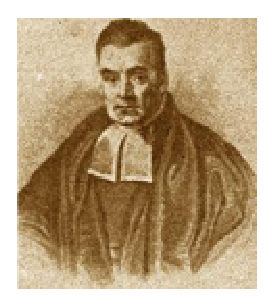
\includegraphics[height=3truecm]{figures/TBayes}
\end{columns}

\end{slide}\begin{slide}
\debut[Normal+improper]
If $x\sim\CN(\theta,1)$ and $\pi(\theta)=\varpi$, constant, 
the pseudo marginal distribution is 
$$
  m(x) =  \varpi \int^{+\infty }_{-\infty} {1 \over \sqrt{ 2\pi} }  
     \exp \left\{-(x-\theta)^2 /2 \right\} d\theta = \varpi
$$
and the posterior distribution of $\theta$ is
$${\Brown{
  \pi (\theta \mid x) = {1 \over \sqrt{ 2\pi}} 
     \exp \left\{ - {(x-\theta )^ 2 \over 2} \right\}  ,
}}$$
i.e., corresponds to ${\cal N}(x,1)$.
\emfarite{independent of $\varpi$}
\fin

\end{slide}\begin{slide}
\slidetitle{Meaningless as probability distribution}

\small\begin{flushright}\begin{quote}
The mistake is to think of them [the non-informative priors]\\
as representing ignorance\\
---Lindley, 1990---
\end{quote}\end{flushright}\normalsize

\pause
\debut Consider a $\theta\sim\CN(0,\tau^2)$ prior. Then
$$
  P^\pi\left( \theta \in [a,b] \right) \longrightarrow 0
$$
when ${\tau\to\infty}$ for any $(a,b)$
\fin

\end{slide}
\begin{slide}\slidetitle{Noninformative prior distributions}

\bigskip
\centerline{\Red{\fbox{\bf What if all we know is that we know ``nothing" ?!}}}

\pause
\bigskip
In the absence of prior information, prior distributions solely derived from the sample distribution \
$f(x|\theta)$

\pause\bigskip
\small\begin{flushright}\begin{quote}
Noninformative priors cannot be expected to represent exactly total ignorance
about the problem at hand, but should rather be taken as reference or 
default priors, upon which everyone could fall
back when the prior information is missing.\\
---Kass and Wasserman, 1996---
\end{quote}\end{flushright}\normalsize


\end{slide}\begin{slide}
\slidetitle{Laplace's prior}

Principle of {\it Insufficient Reason} (Laplace)
$$
\Theta = \{\theta_1,\cdots,\theta_p\}  \hspace{1cm}  \pi(\theta_i)=1/p
$$

\pause\smallskip
Extension to continuous spaces
{\Red{
$$
\pi(\theta) \propto 1
$$
}}
\emfarite{Lebesgue measure}

\end{slide}
\begin{slide}
\slidetitle{\Blue{\sf Who's Laplace?}}

\begin{block}{\BrickRed{{\bf Pierre Simon de Laplace (1749--1827)}}}
\begin{columns}\column{.55\textwidth}
French mathematician and astronomer born in Beaumont en Auge (Normandie)
who formalised mathematical astronomy in {\em M\'ecanique C\'eleste}. 
Survived the French revolution, the Napoleon Empire (as a comte!), and
the Bourbon restauration (as a marquis!!).

\column{.4\textwidth}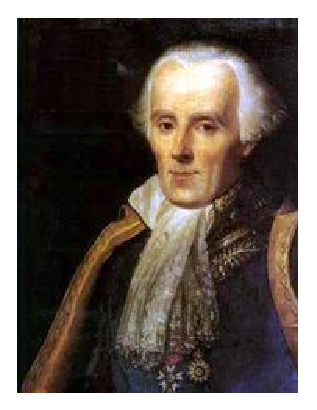
\includegraphics[height=3truecm]{figures/Laplace}
\end{columns}

\medskip
\pause
In {\em Essai Philosophique sur les Probabilit\'es}, Laplace set out a mathematical system of inductive 
reasoning based on probability, precursor to Bayesian Statistics. 
\end{block}

\end{slide}\begin{slide}
\slidetitle{Laplace's problem}

\begin{itemize}
\item  Lack of reparameterization invariance/coherence
{\Brown{
$$
\pi(\theta)\propto 1,\quad\text{and}\quad
\psi = e^{\theta}  \hspace{0.5cm}  \pi(\psi)={1\over\psi} \neq 1 \quad (!!)
$$
}}

\pause\item  Problems of properness
$$
{\Brown{
x\sim {\cal N}(\mu,\sigma^2),  \hspace{1cm}  \pi(\mu,\sigma)=1
}}
$$
$$
{\Brown{
\begin{array}{llll}
\space & \pi(\mu,\sigma|x) &\propto& e^{-(x-\mu)^2/2\sigma^2} 
\sigma^{-1} \\
\Rightarrow & \pi(\sigma|x) &\propto& 1 \qquad (!!!)
\end{array}
}}
$$
\end{itemize}

\end{slide}\begin{slide}
\slidetitle{Jeffreys' prior}

\begin{columns}\column{.55\textwidth}
Based on Fisher information
$$\BrickRed{
I^F (\theta) = \e_{\theta}\left[{\partial\log\ell\over\partial\theta^t}\;
              {\partial\log\ell\over\partial\theta}\right]
}$$
\column{.45\textwidth}
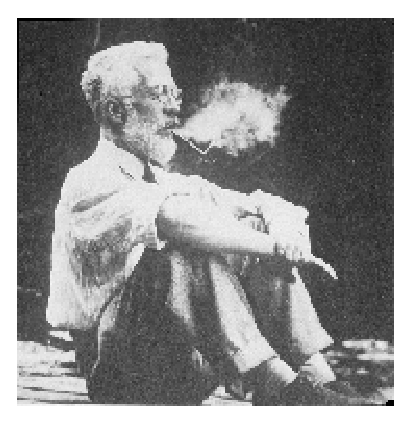
\includegraphics[height=3truecm]{figures/RonSmoke}\\
\small{\bf Ron Fisher (1890--1962)}\normalsize
\end{columns}

\pause
the Jeffreys prior distribution is 
{\Red{
$$
  \pi^J (\theta ) \propto |I^F (\theta)|^{1/2}
$$
}}

\end{slide}\begin{slide}
\slidetitle{\Blue{\sf Who's Jeffreys?}}

\begin{block}{{\BrickRed{{\bf Sir Harold Jeffreys (1891--1989) }}}}
\begin{columns}\column{.5\textwidth}
English mathematician, statistician, geophysicist, and astronomer. Founder of English Geophysics \&\
originator of the theory that the Earth core is liquid.

\pause
Formalised Bayesian methods for the analysis of geophysical data and ended up writing {\em Theory
of Probability}
\column{.4\textwidth}
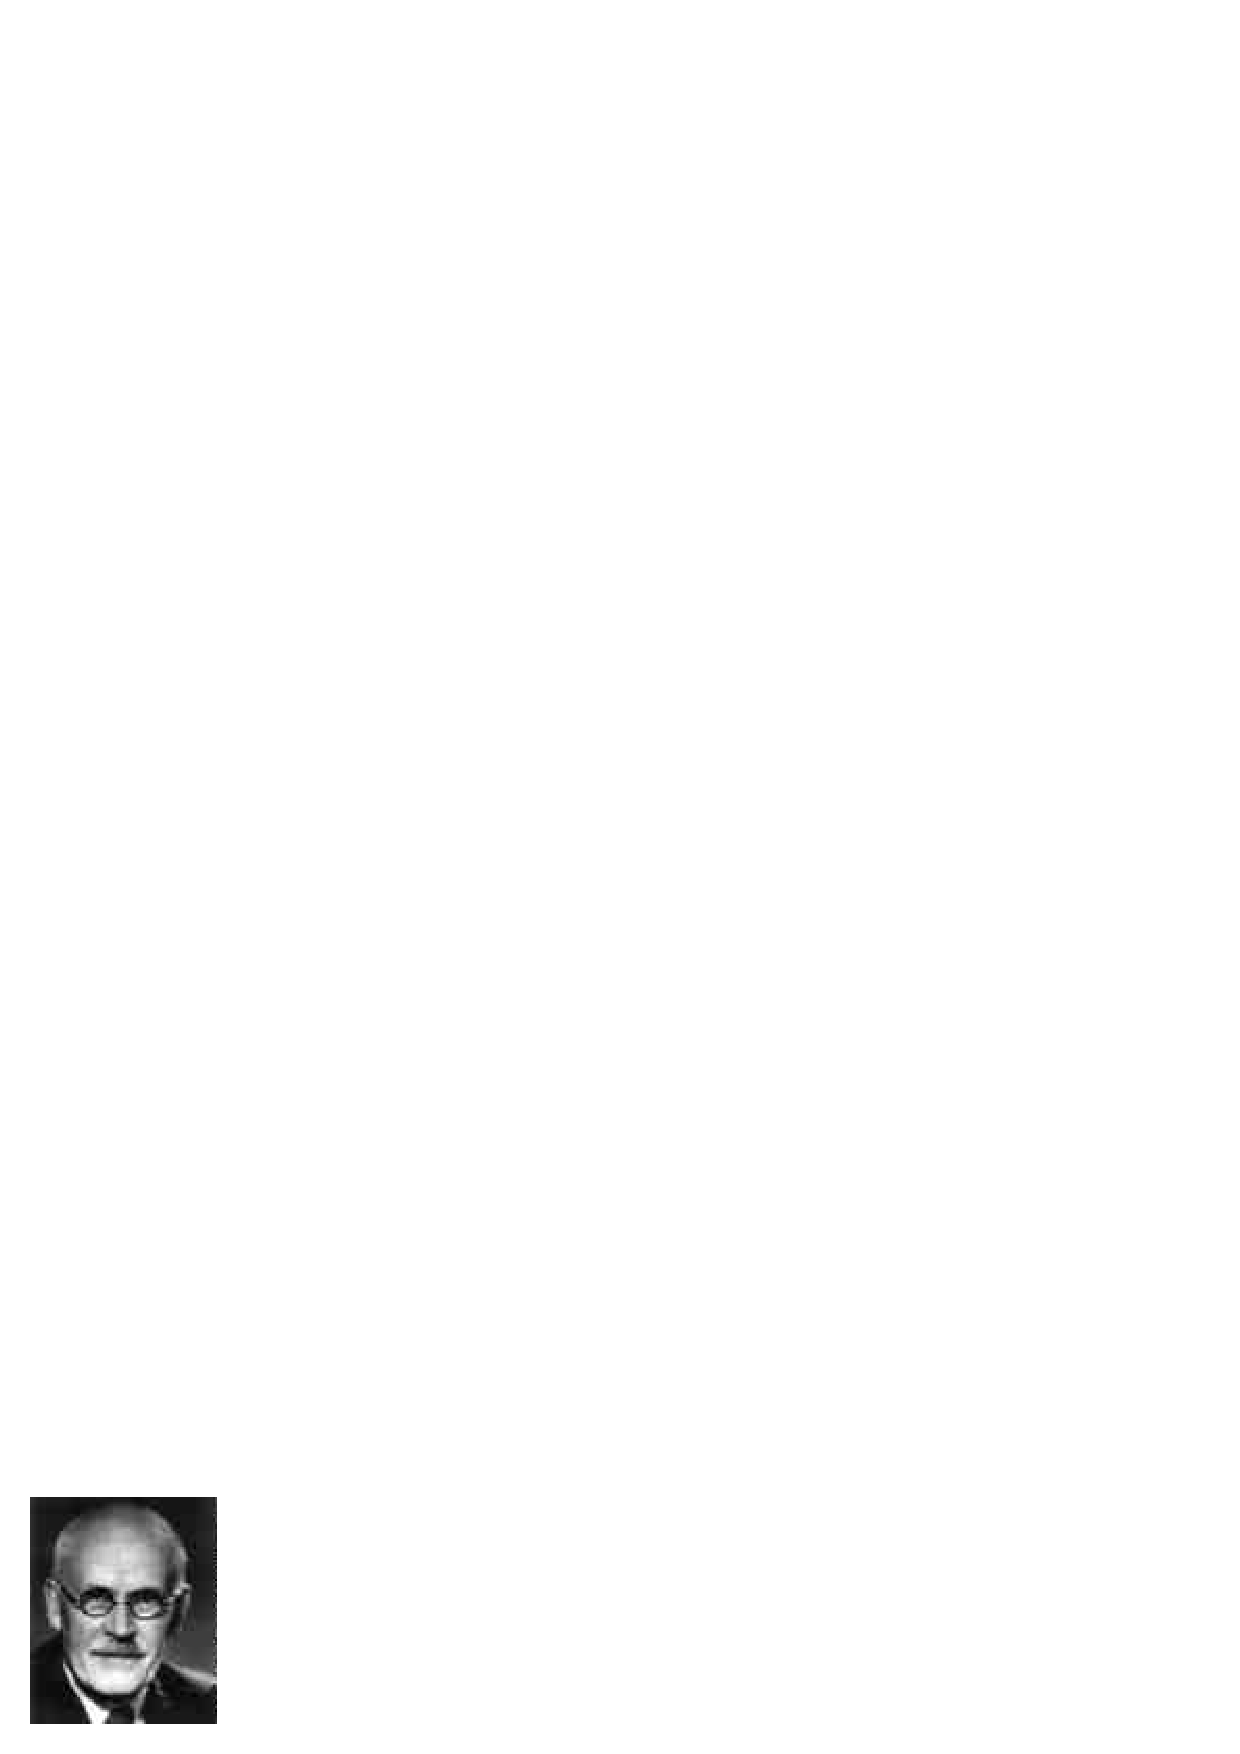
\includegraphics[height=3.5truecm]{figures/Jeffreys}
\end{columns}\end{block}

\end{slide}\begin{slide}
\slidetitle{Pros \&\ Cons}

\begin{itemize}    
\item  Relates to information theory
\pause
\item  Agrees with most invariant priors
\pause
\item  Parameterization invariant
\pause
\item  Suffers from dimensionality curse
\end{itemize}    

\end{slide}
\subsection{Bayesian estimation}
\begin{slide}
\slidetitle{Evaluating estimators}

Purpose of most inferential studies:
to provide the statistician/client with a
{\it decision} $d\in\CD$

\pause
Requires an evaluation criterion/{\sf loss function} for decisions and estimators
{\Red{$$
\Lrm(\theta,d)
$$}}

\pause\bigskip
{\RedOrange{\bf
There exists an axiomatic derivation
of the existence of a loss function.
}}
\rightline{\Brown{\sf [DeGroot, 1970]}}

%\end{slide}\begin{slide}
%\slidetitle{Bayesian \DT}

%Three spaces/factors:
%\begin{itemize}
%\item[(1)] On $\CX$, distribution for the observation,    $f(x|\theta)$;
%\item[(2)] On $\Theta$, prior distribution for the parameter,       $\pi(\theta)$;
%\item[(3)] On $\Theta\times\CD$, 
           %loss function associated with the decisions, $\Lrm(\theta,\delta)$;
%\end{itemize}

\end{slide}\begin{slide}
\slidetitle{Loss functions}

Decision procedure $\delta^\pi$ usually called
{\RedViolet{\sf estimator}}\\ (while its {\it value} $\delta^\pi(x)$
is called {\RedViolet{\sf estimate}} of $\theta$)

\pause\bigskip
Impossible to uniformly minimize  (in $d$)  the loss function
$$
\Lrm(\theta,d)
$$
when $\theta$ is unknown

%\end{slide}\begin{slide}
%\slidetitle{Frequentist Principle}

%Average loss (or {\RedViolet{\sf frequentist risk}})
%\begin{eqnarray*}
%R(\theta,\delta) & = & \BE_\theta \lbrack \Lrm (\theta
%,\delta(x))\rbrack \\
	%& = & \int_{\cal X} \Lrm(\theta,\delta(x))f(x|\theta) \,dx
%\end{eqnarray*}

%\medskip\pause
%{\BurntOrange{\bf Principle}} Select the best estimator based on the risk function

%\end{slide}\begin{slide}
%\slidetitle{Difficulties with frequentist paradigm}

%\begin{enumerate}
%\item Error averaged over the different values
%of $x$ proportionally to the density $f(x|\theta)$:
%not so appealing for a client, who wants
%optimal results for {\Red{\bf her}} data $x$!
%\pause\item Assumption of repeatability of experiments not always grounded.
%\pause\item $R(\theta, \delta)$ is a function of $\theta$: there is no
%total ordering on the set of procedures. 
%\end{enumerate}

\end{slide}\begin{slide}
\slidetitle{Bayesian estimation}
{\BurntOrange{\bf Principle}} Integrate over the space $\Theta$
to get the posterior expected loss
\begin{eqnarray*}
      & = & \BE^\pi[\Lrm(\theta,d)|x] \\
      & = & \int_{\Theta} \Lrm(\theta,d) \pi(\theta|x)\, d\theta,
\end{eqnarray*}
and minimise in $d$

\end{slide}\begin{slide}
\slidetitle{Bayes estimates}
{\Blue{
\begin{block}{Bayes estimator}
A {\Red{\em Bayes estimate}}\ associated with a prior distribution $\pi$ and a loss function $\Lrm$ is 
$$
  \arg\min_d \BE^\pi[\Lrm(\theta,d)|x] \,.
$$
\end{block}
}}

\end{slide}
%\subsubsection{Usual loss functions}\label{sec:2.5}
\begin{slide}
\slidetitle{The quadratic loss}

\begin{columns}\column{.6\textwidth}
Historically, first loss function (Legendre, Gauss, Laplace)
\[
	\Lrm (\theta ,d)  =  (\theta -d)^2
\]
\column{.4\textwidth}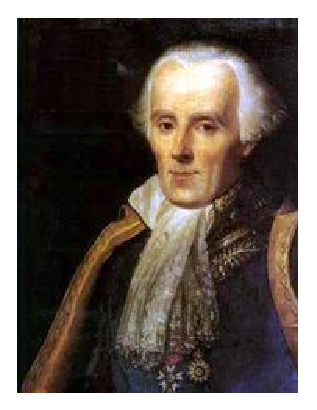
\includegraphics[height=3truecm]{figures/Laplace}
\end{columns}


%\end{slide}\begin{slide}
%\slidetitle{Proper loss}

\pause\smallskip {\RawSienna{
The Bayes estimate $\delta^\pi(x)$ associated with the prior $\pi$ and with the quadratic loss
is the posterior expectation
$$
\delta^\pi(x)  =  \BE^\pi[\theta|x]  = 
	{\int_\Theta \theta f(x|\theta)\pi(\theta) \,d\theta \over
		\int_\Theta f(x|\theta)\pi(\theta) \,d\theta} .
$$
}}

\end{slide}\begin{slide}
\slidetitle{The absolute error loss}

Alternatives to the quadratic loss:
\[
\Lrm(\theta,d)  =  \mid \theta-d\mid,
\]
or
\begin{eqnarray*}
\Lrm_{k_1,k_2} (\theta ,d)  =  \begin{cases} k_2(\theta -d) &
   \hbox{if }\theta  > d , \cr
			k_1(d-\theta )  & \hbox{otherwise.} \cr
			\end{cases}
\end{eqnarray*}

\pause
{\RawSienna{
Associated Bayes estimate is
$(k_2/(k_1+k_2))$ fractile of $\pi(\theta|x)$
}}

\end{slide}\begin{slide}
\slidetitle{MAP estimator}

With no loss function, consider using
the {\RedViolet{\sf maximum a posteriori (MAP) estimator}}
$$
\arg\max_\theta \ell(\theta|x)\pi(\theta)
$$

\smallskip\pause
%\end{slide}\begin{slide}
%\slidetitle{Motivations}
\begin{itemize}
\item Penalized likelihood estimator
\pause
\item Further appeal in restricted parameter spaces
\end{itemize}

\end{slide}\begin{slide}
\debut[Binomial probability]
Consider $x|\theta\sim{\cal B}(n,\theta)$. 

Possible priors:
$$
\pi^J (\theta) = {1 \over B(1/2,1/2)} \theta^{-1/2} (1-\theta)^{-1/2}\,,
$$
$$
\pi_1(\theta) = 1 \quad \hbox { and } \quad \pi_ 2(\theta) = \theta^{-1}(1-\theta)^{-1} \,.
$$
\pause
Corresponding MAP estimators:
\small
\begin{eqnarray*}
\delta^{\pi_J} (x) &=& \max \left({x-1/2 \over n - 1} , 0 \right) , \\
\delta^{\pi_1} (x) &=&  x / n , \\
\delta^{\pi_2} (x) &=& \max \left({x-1 \over n-2} , 0 \right) .
\end{eqnarray*}
\normalsize
\fin

\end{slide}\begin{slide}
\slidetitle{Not always appropriate}
\debut[Fixed MAP] Consider  
$$
f(x | \theta ) = {1 \over \pi}  \left[1+(x-\theta )^2 \right]^{-1},
$$
and $\pi(\theta)={1 \over 2} e^{-|\theta |}$.
\pause
Then the MAP estimate of $\theta$ is always
\[\Brown{
  \delta^\pi (x) = 0
}\]
\fin

\end{slide}
\subsection{Confidence regions}\begin{slide}
\slidetitle{Credible regions}

Natural confidence region: Highest posterior density (HPD) region
$$
C_\alpha^\pi =  \lbrace \theta;\pi(\theta |x)>k_\alpha\rbrace
$$
%\rightline{\Purple{\sf Highest posterior density (HPD) region}}

\pause
\begin{block}{Optimality}
\begin{columns}\column{.55\textwidth}
The HPD regions give the highest probabilities of containing $\theta$ for a given volume
\column{.4\textwidth}
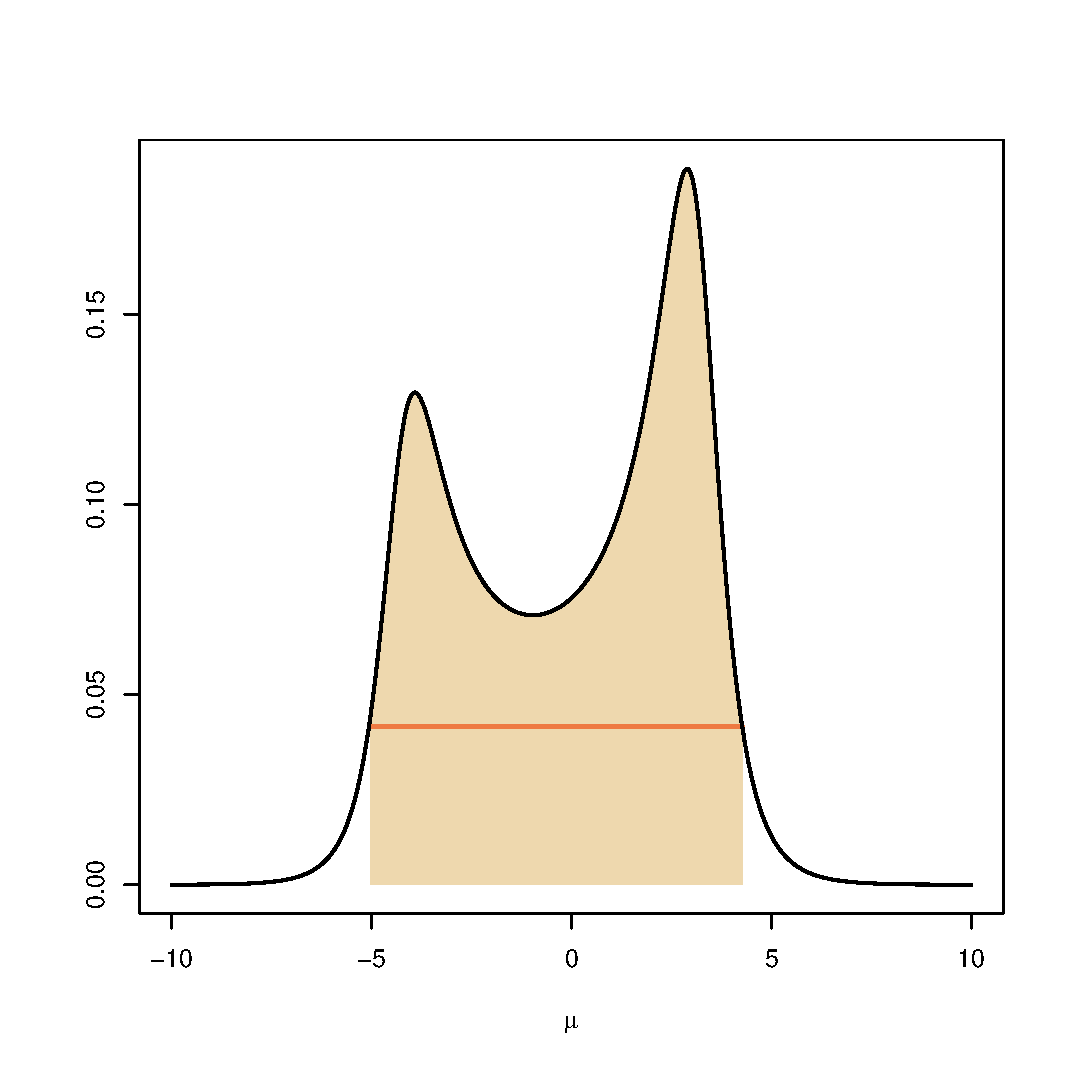
\includegraphics[width=4cm,height=4truecm]{figures/2cau}
\end{columns}
\end{block}

\end{slide}\begin{slide}
\debut If the posterior distribution of $\theta$ is 
${\cal N}(\mu(x),\allowbreak\omega^{-2})$ with $\omega^2=\tau^{-2}+\sigma^{-2}$ and 
$\mu(x)= \tau^2 x/(\tau^2+\sigma^2)$,
then
$$
C^\pi_\alpha  =  \left[\mu(x)-k_{\alpha} \omega^{-1}, \mu(x)+k_{\alpha} 
\omega^{ -1} \right],
$$
where $ k_\alpha $ is the $\alpha/2$-quantile of ${\cal N}(0,1)$. 

\pause
If $\tau$ goes to $+\infty$,
$$
C_\alpha^\pi =\left[x-k_{\alpha} \sigma , x+k_{\alpha} \sigma \right] ,
$$
the ``usual" (classical) confidence interval
\fin

\end{slide}
%\subsection{Normal model again}
\begin{slide}\slidetitle{Full normal}

Under [almost!] {\em Jeffreys prior} prior 
$$
\pi(\mu,\sigma^2)=1/\sigma^2,
$$
posterior distribution of $(\mu,\sigma)$
\small\begin{eqnarray*}
\mu|\sigma,{\bar x},s_x^2 & \sim & \CN\left({\bar x},{\sigma^2\over n}\right), \nonumber \\
\sigma^2|{\bar x},s_x^2   & \sim & {\cal IG}\left({n-1\over 2},{s_x^2\over 2}\right).
\end{eqnarray*}\normalsize

\smallskip\pause
Then
\begin{eqnarray*}\small
\pi(\mu|{\bar x},s_x^2)  & \propto & \int \omega^{1/2}\,\exp-\omega\frac{n({\bar x}-\mu)^2}{2}\,\omega^{(n-3)/2}\,\exp\{-\omega s_x^{2}/2\}\,\text{d}\omega \\
	                     & \propto & \left[ s_x^2 + n({\bar x}-\mu)^2 \right]^{-n/2}
\end{eqnarray*}\normalsize
\emfarite{$\mathcal{T}_{n-1}$ distribution}

\end{slide}\begin{slide}\slidetitle{Normal credible interval}

Derived credible interval on $\mu$
$$
[\bar x - t_{\alpha/2,n-1}s_x\big/\sqrt{n(n-1)},\bar x +t_{\alpha/2,n-1}s_x\big/\sqrt{n(n-1)}]
$$

\medskip\pause
\begin{block}{{\sf normaldata}}
Corresponding $95\%$ confidence region for $\mu$ 
$$
[-0.070,-0.013,]
$$ 
Since $0$ does not belong to this interval, reporting 
a significant decrease in the number of larcenies between 
1991 and 1995 is acceptable
\end{block}

\end{slide}
\subsection{Testing}\begin{slide}
%\subsubsection{The $0-1$ loss}
\slidetitle{Testing hypotheses}

Deciding about validity of assumptions or restrictions on
the parameter $\theta$ from the data, represented as
$$\BrickRed{
H_0:\theta \in\Theta_0 \quad\text{versus}\quad H_1:\theta \not\in\Theta_ 0
}$$

\pause
Binary outcome of the decision process: {\em accept} [coded by 1] or {\em reject\/} [coded by 0]
$$\BrickRed{
  \CD  =  \lbrace 0,1 \rbrace
}$$

\pause
Bayesian solution formally very close from a likelihood ratio test statistic, but
numerical values often strongly differ from classical solutions

\end{slide}\begin{slide}
\slidetitle{The $0-1$ loss}

Rudimentary loss function
$$
L (\theta ,d)  =  \begin{cases} 1-d & \hbox{if }\theta \in \Theta_0 \cr
			  d    &  \hbox{otherwise,} \cr \end{cases}
$$

Associated Bayes estimate
$$\RawSienna{
\delta^\pi(x) = \begin{cases} 1 &\hbox{if }P^\pi(\theta\in\Theta_0|x)
                        >\displaystyle{\frac{1}{2}},\cr
        0 & \hbox{otherwise.} \end{cases}
}$$

\pause
Intuitive structure

\end{slide}\begin{slide}
\slidetitle{Extension} 

Weighted $0-1$ (or $a_0-a_1$) loss
\begin{equation*}
\Lrm(\theta, d) = \begin{cases} 0 & \hbox{if } d=\BI_{\Theta_0}(\theta), \cr
           a_0 & \hbox{if }\theta\in\Theta_0\hbox{ and } d=0, \cr
           a_1 & \hbox{if }\theta\not\in\Theta_0\hbox{ and }d=1, \cr\end{cases}
\end{equation*}

\pause
\begin{block}{Associated Bayes estimator}
$$\RawSienna{
\delta^\pi(x) = \begin{cases} 1 &\hbox{if }P^\pi(\theta\in\Theta_0|x)
                        >\displaystyle{a_1\over a_0+a_1},\cr
	0 & \hbox{otherwise.} \end{cases}
}$$
\end{block}
\end{slide}\begin{slide}
\debut[Normal-normal] For $x\sim \CN(\theta,\sigma^2)$ 
and $\theta\sim\CN(\mu,\tau^2)$, $\pi(\theta|x)$ is 
$\CN(\mu(x),\omega^2)$ with
$$
\mu(x) = {\sigma^2\mu+\tau^2 x\over \sigma^2 +\tau^2} \quad \hbox{ and }
\quad \omega^2={\sigma^2\tau^2 \over \sigma^2+\tau^2}.
$$
\pause
To test $H_0:\,\theta<0$, we compute
\begin{eqnarray*}
P^\pi(\theta<0|x) &=& P^\pi\left({\theta-\mu(x)\over \omega} < 
			{-\mu(x)\over \omega} \right) \\
		&=& \Phi\left(-\mu(x)/ \omega \right). 
\end{eqnarray*}
\fin

\end{slide}\begin{slide}
\debut[Normal-normal (2)] If $z_{a_0,a_1}$ is the $a_1/(a_0+a_1)$ quantile, i.e., 
$$\Phi(z_{a_0,a_1})=a_1/(a_0+a_1)\,,$$ 
$H_0$ is accepted when
$$
  -\mu(x) > z_{a_0,a_1} \omega,
$$
the upper acceptance bound then being 
$$\BrickRed{
x \le - {\sigma^2 \over \tau^2} \mu - (1+{\sigma^2\over \tau^2}) 
\omega z_{a_0,a_1}.
}$$
\fin

\end{slide}\begin{slide}
\slidetitle{Bayes factor}
Bayesian testing procedure depends on $P^\pi (\theta \in \Theta_0|x)$ 
or alternatively on the \Blue{{\bf Bayes factor}}
$$
\BrickRed{
B^\pi_{10} = \frac{\left\{ P^\pi(\theta \in \Theta_1|x) / P^\pi(\theta \in \Theta_0|x) \right\} 
}{ \left\{ P^\pi(\theta \in \Theta_1)/ P^\pi(\theta \in \Theta_0) \right\} }
}$$
in the absence of loss function parameters $a_0$ and $a_1$

\end{slide}\begin{slide}
\slidetitle{Associated reparameterisations}

Corresponding models ${\cal M}_1$ vs. ${\cal M}_0$ compared via
$$
B_{10}^\pi = \displaystyle{ {P^\pi ({\cal M}_1|x) \over P^\pi ({\cal M}_0|x)} \bigg/
{P^\pi ({\cal M}_1) \over P^\pi  ({\cal M}_0)} } 
$$

\pause
If we rewrite the prior as 
\centerline{$\pi(\theta) = \hbox{Pr}(\theta\in\Theta_1)\times\pi_1(\theta) +
		\hbox{Pr}(\theta\in\Theta_0)\times\pi_0(\theta)$}
then
$$
B_{10}^\pi = { \displaystyle{\int f(x|\theta_1) \pi_1(\theta_1) \text{d}\theta_1} }\bigg/{
\displaystyle{\int f(x|\theta_0) \pi_0(\theta_0) \text{d}\theta_0} } = m_1(x)/m_0(x)
$$
\emfarite{{\bf Akin to likelihood ratio}}

\end{slide}\begin{slide}
\slidetitle{Jeffreys' scale}
\begin{columns}\column{.65\textwidth}
\begin{enumerate}
   \item if $\log_{10} (B^\pi_{10})$ varies between $0$ and $0.5$,
           the evidence against $H_0$ is {\it poor},
   \item if it is between $0.5$ and $1$, it is is {\it substantial},
   \item if it is between $1$ and $2$, it is {\it strong}, and
   \item if it is above $2$ it is {\it decisive}.
\end{enumerate}
\column{.3\textwidth}
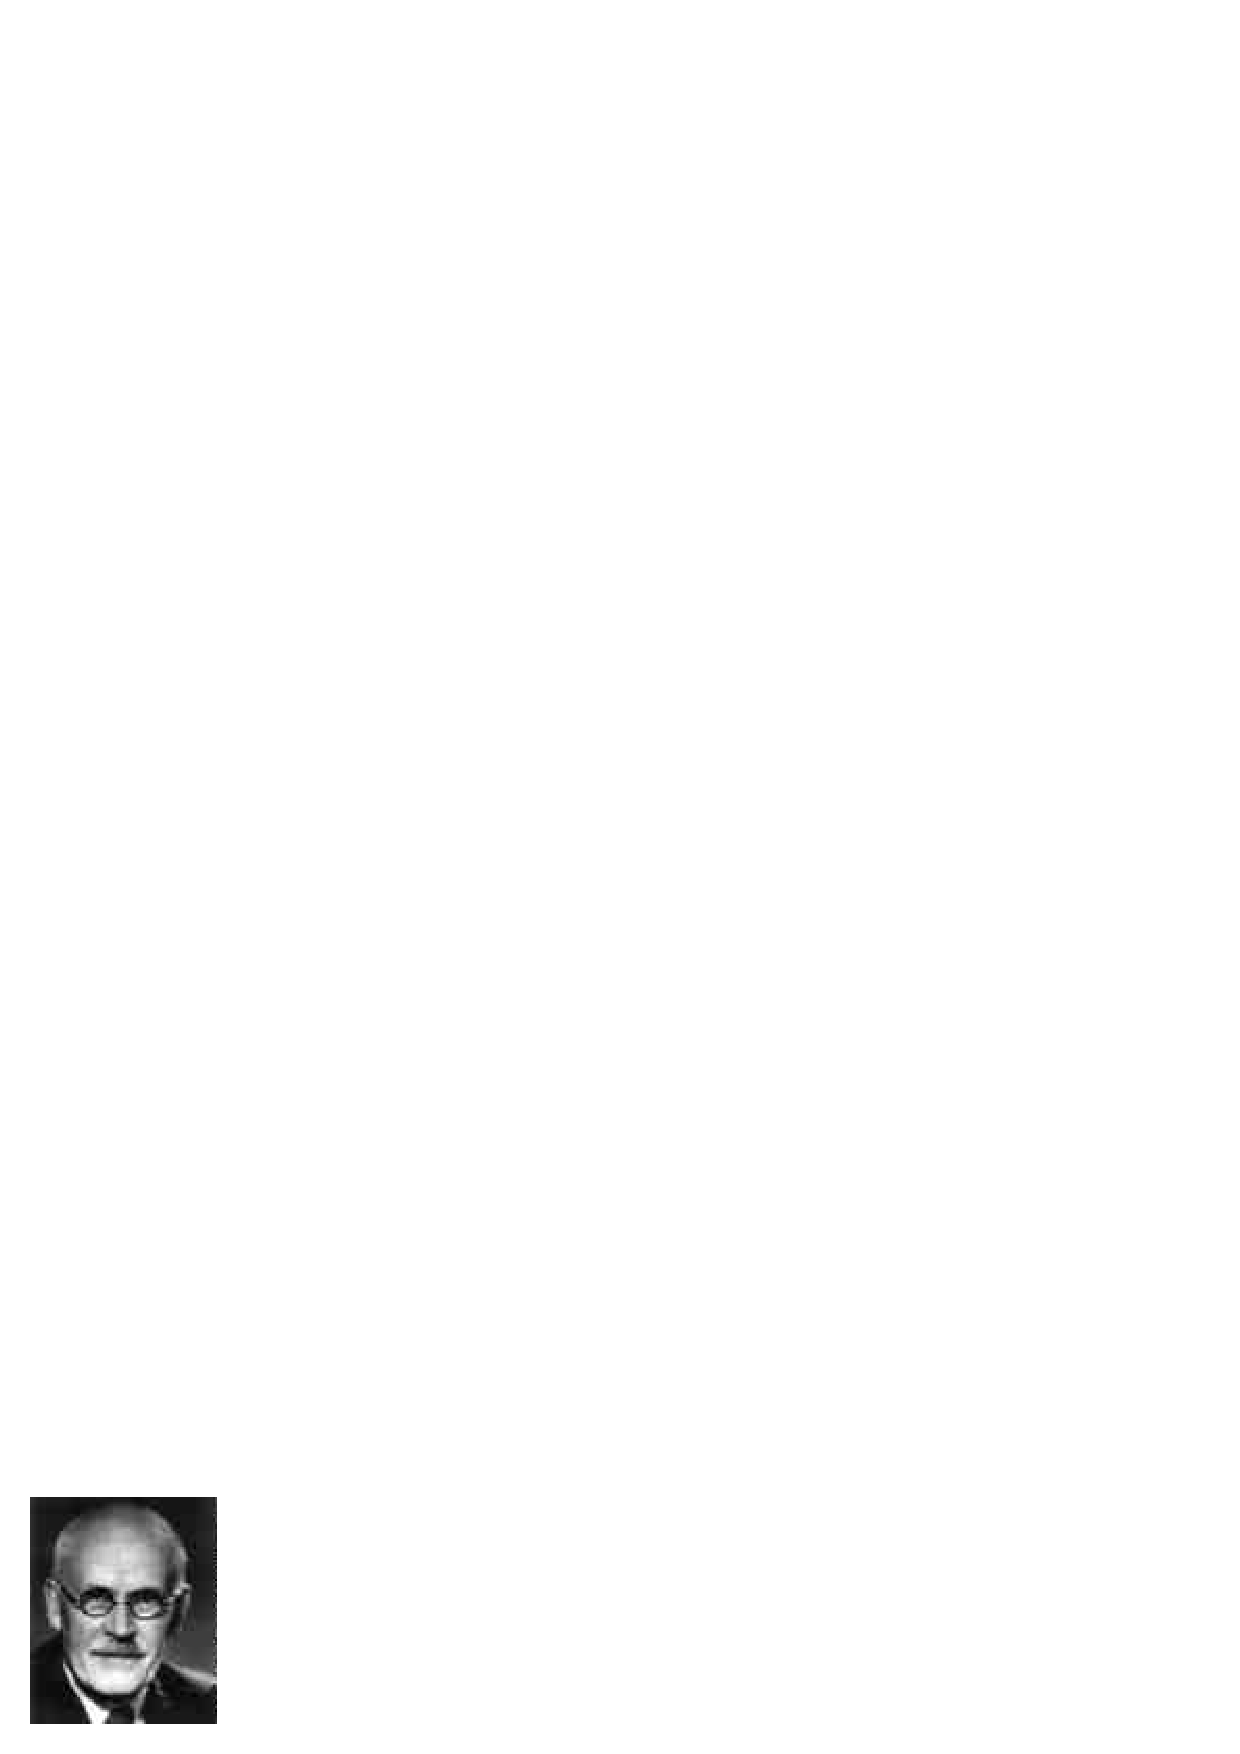
\includegraphics[height=3truecm]{figures/Jeffreys}
\end{columns}

\end{slide}\begin{slide}
\slidetitle{Point null difficulties}

If $\pi$ absolutely continuous, 
$$P^\pi(\theta=\theta_0)=0\ldots$$

\pause
\vglue 1truecm
\centerline{\BurntOrange{\fbox{{\bf How can we test $H_0:\theta=\theta_0$?!}}}}

\end{slide}\begin{slide}
\slidetitle{New prior for new hypothesis}

Testing point null difficulties requires a modification of the prior distribution
so that 
$$\Brown{
\pi(\Theta_0)>0 \quad\hbox{and}\quad \pi(\Theta_1)>0
}$$
(hidden information) or
$$\Brown{
\pi(\theta) = P^\pi (\theta\in\Theta_0)\times\pi_0(\theta) +
                P^\pi (\theta\in\Theta_1)\times\pi_1(\theta)
}$$


\pause
\emfarite{E.g., when $\Theta_0=\{\theta_0\}$, $\pi_0$ is Dirac mass at $\theta_0$}

\end{slide}\begin{slide}
\slidetitle{Posteriors with Dirac masses}

If $H_0: \ \theta=\theta_0$ $(=\Theta_1)$, 
$$
\rho = P^\pi (\theta=\theta_0) \quad\hbox{and}\quad
\pi(\theta) = \rho \BI_{\theta_0}(\theta)+ (1-\rho) \pi_1(\theta)
$$
then
\begin{align*}
\pi(\Theta_0|x) &= {f(x|\theta_0)\rho \over 
		\int f(x|\theta)\pi(\theta)\,d\theta} \\
 &= \BrickRed{{f(x|\theta_0)\rho \over f(x|\theta_0)\rho + (1-\rho) m_1(x)}}
\end{align*}
with
$$
m_1(x)=\int_{\Theta_1} f(x|\theta)\pi_1(\theta)\,d\theta.
$$

\end{slide}\begin{slide}
\debut[Normal-normal] For $x\sim \CN(\theta,\sigma^2)$ and $\theta\sim\CN(0,\tau^2)$,
to test of $H_0:\theta=0$ requires a modification of the prior, with
$$\RawSienna{
\pi_1(\theta) \propto e^{-\theta^2/2\tau^2} \mathbb{I}_{\theta\ne 0}
}$$
and $\pi_0(\theta)$ the Dirac mass in $0$

\pause
Then
\begin{eqnarray*}
{m_1(x)\over f(x|0)} &=&  {\sigma\over \sqrt{\sigma^2+\tau^2}}
	{e^{-x^2/2(\sigma^2+\tau^2)} \over e^{-x^2/2\sigma^2}} \\
      &=&  \sqrt{{\sigma^2\over\sigma^2+\tau^2}} \exp\left\{
	   {\tau^2x^2\over 2\sigma^2(\sigma^2+\tau^2)} \right\}, 
\end{eqnarray*}
\fin

\end{slide}\begin{slide}
\debut[cont'd]
and
$$
\pi(\theta=0|x) = \left[ 1+{1-\rho\over \rho} \sqrt{{\sigma^2\over
\sigma^2+\tau^2}} \exp\left({\tau^2x^2\over 2\sigma^2(\sigma^2+\tau^2)}\right)
\right]^{-1}.
$$

For $z=x/\sigma$ and $\rho=1/2$:
 
\centerline{
\MidnightBlue{\begin{tabular}{|c|c|c|c|c|}
\hline
$ z $ & $ 0$ & $ 0.68 $ & $ 1.28$ & $ 1.96 $ \cr
\hline
$ \pi(\theta=0| z,\tau=\sigma) $ & $ 0.586$ & $ 0.557 $ & $ 0.484$ & $ 0.351 $ \cr
$ \pi(\theta =0|z,\tau=3.3\sigma) $ & $ 0.768$ & $ 0.729 $ & $ 0.612$ & $ 0.366 $ \cr
\hline
\end{tabular}}}
\fin

\end{slide}\begin{slide}
\slidetitle{Banning improper priors}

Impossibility of using improper priors for testing!

\medskip\pause
\Brown{{\bf Reason:}} When using the representation
$$
\pi(\theta) = P^\pi (\theta\in\Theta_1)\times\pi_1(\theta) +
              P^\pi (\theta\in\Theta_0)\times\pi_0(\theta)
$$
$\pi_1$ and $\pi_0$ must be normalised

\end{slide}\begin{slide}
\debut[Normal point null] When $x\sim \CN(\theta,1)$ and $H_0:\ \theta=0$, for
the improper prior $\pi(\theta)=\Red{{\mathbf 1}}$, the prior is transformed as
$$
\pi(\theta)  = {1\over 2} \BI_{0}(\theta) + {1\over 2} \cdot \Red{{\mathbf \BI_{\theta\ne 0}}},
$$
and
\begin{eqnarray*}
\pi(\theta=0|x) &=& {e^{-x^2/2}\over e^{-x^2/2}+\int_{-\infty}^{+\infty}
   e^{-(x-\theta)^2/2} \,d\theta} \\
&=&  {1 \over 1+\sqrt{2\pi} e^{x^2/2} }.
\end{eqnarray*}
\fin

\end{slide}\begin{slide}
\debut[Normal point null (2)] 
\RawSienna{{\bf Consequence:}} 
$H_0$ is bounded from above by 
$$
\pi(\theta=0|x) \le 1/(1+\sqrt{2\pi})=0.285
$$
\MidnightBlue{\centerline{
\begin{tabular}{|c|c|c|c|c|c|}
\hline
$x $ & $ 0.0$ & $ 1.0 $ & $ 1.65$ & $ 1.96 $ & $ 2.58 $ \cr
\hline
$ \pi(\theta=0| x)$ & $0.285 $ &$0.195$ & $0.089 $ & $0.055$ & $0.014$ \cr
\hline
\end{tabular}
}}
\fin

\medskip
\RawSienna{{\bf Regular tests:}}
Agreement with the classical $p$-value (but...)

\end{slide}\begin{slide}
\debut[Normal one-sided] For $x\sim\CN(\theta,1)$, $\pi(\theta)=1$, 
and $H_0:\ \theta\le 0$ to test versus $H_1: \theta>0$
$$
\pi(\theta\le 0|x) =  {1\over \sqrt{2\pi} } \int_{-\infty}^0 
	e^{-(x-\theta)^2/2} \,d\theta =  \Phi(-x). 
$$
The generalized Bayes answer is also the {\it $p$-value}
\fin

\pause\medskip
\begin{block}{{\sf normaldata}}
If $\pi(\mu,\sigma^2)=1/\sigma^2$, 
$$
\pi(\mu\ge 0|x) = 0.0021
$$
since $\mu|x\sim\mathscr{T}_{89}(-0.0144,0.000206)$.
\end{block}

\end{slide}\begin{slide}
\slidetitle{Jeffreys--Lindley paradox}

\BurntOrange{{\sffamily\bfseries Limiting arguments not valid in testing settings:}}
Under a conjugate prior
$$
\pi(\theta=0|x) = \left\{ 1+{1-\rho\over \rho} 
	\sqrt{{\sigma^2\over \sigma^2+\tau^2}} \exp
  \left[{\tau^2x^2\over 2\sigma^2(\sigma^2+\tau^2)}\right] \right\}^{-1} ,
$$
which converges to \BrickRed{$1$} when $\tau$ goes to $+\infty$, 
\Red{{\bf for every $x$}}

\medskip\pause
Difference with the ``noninformative'' answer 
$$
[1+\sqrt{2\pi}\exp(x^2/2)]^{-1}
$$
\emfarite{\BrickRed{{\Large $\lightning$} Invalid answer}}

\end{slide}\begin{slide}
\slidetitle{Normalisation difficulties}
If $g_0$ and $g_1$ are $\sigma$-finite measures 
on the subspaces $\Theta_0$ and $\Theta_1$, the choice of the normalizing constants 
influences the Bayes factor: 

\BurntOrange{{\bf If $g_i$ replaced by $c_ig_i$ $(i=0,1)$, 
Bayes factor multiplied by \Red{$c_0/c_1$}}}

\pause
\debut If the Jeffreys prior is uniform and $g_0=c_0$, $g_1=c_1$, 
\small
\begin{eqnarray*}
\pi(\theta\in\Theta_0|x) &=& {\rho c_0\int_{\Theta_0} f(x|\theta)\,d\theta
	    \over \rho c_0\int_{\Theta_0} f(x|\theta)\,d\theta +
	   (1-\rho)c_1\int_{\Theta_1} f(x|\theta)\,d\theta }\\
&=& {\rho \int_{\Theta_0} f(x|\theta)\,d\theta
            \over \rho \int_{\Theta_0} f(x|\theta)\,d\theta +
           (1-\rho)\Red{\mathbf{[c_1/c_0]}}\int_{\Theta_1} f(x|\theta)\,d\theta }
\end{eqnarray*}
\normalsize
\fin

\end{slide}
\subsection{Monte Carlo integration}\begin{slide}
\slidetitle{Monte Carlo integration}

Generic problem of evaluating an integral
\begin{displaymath}\Brown{
    {\mathfrak{I}} = \BE_f[h(X)] = \int_{\CX} \; h(x) \; f(x) \; dx \;
}\end{displaymath}
where $\CX$ is uni- or multidimensional, $f$ is a closed form, partly closed form, or implicit density,
and $h$ is a function

\end{slide}\begin{slide}
\slidetitle{Monte Carlo Principle}
Use a sample $(x_1,\ldots,x_{m})$  from the density $f$ 
to approximate the integral ${\mathfrak{I}}$ by the empirical average
$$
  {\overline{h}}_{m} = {1\over m} \; \sum_{j=1}^{m} \; h(x_{j})
$$

\medskip\pause
Convergence of the average 
$$
  {\overline{h}}_{m}  \longrightarrow \BE_f[h(X)]
$$
by the {\Blue{\bf Strong Law of Large Numbers}}

\end{slide}\begin{slide}
\slidetitle{Bayes factor approximation}

For the normal case 
\begin{eqnarray*}
x_1,\ldots,x_n&\sim&\mathscr{N}(\mu+\xi,\sigma^2)\\
y_1,\ldots,y_n&\sim&\mathscr{N}(\mu-\xi,\sigma^2)\\ 
\text{and} && H_0:\xi=0
\end{eqnarray*}
under prior 
$$
\pi(\mu,\sigma^2)=1/\sigma^2 \quad\text{ and }\quad \xi\sim\mathscr{N}(0,1)
$$
\small
$$
B^\pi_{01} = \frac{ \left[ (\bar x-\bar y)^2+S^2 \right]^{-n+1/2} }{
\int\,\left[ (2\xi-\bar x-\bar y)^2+S^2 \right]^{-n+1/2} \,e^{-\xi^2/2}\,\hbox{d}\xi/\sqrt{2\pi}}
$$
\normalsize

\end{slide}\begin{slide}
\slidetitle{Example}
\begin{block}{{\sf CMBdata}}
Simulate $\xi_1,\ldots,\xi_{1000}\sim\mathscr{N}(0,1)$ and approximate $B^\pi_{01}$ with
\small
$$
{\widehat{B^\pi_{01}}} = \frac{ \left[ (\bar x-\bar y)^2+S^2 \right]^{-n+1/2} }{
\frac{1}{1000}\,\sum_{i=1}^{1000} \left[ (2\xi_i-\bar x-\bar y)^2+S^2 \right]^{-n+1/2} } = 89.9
$$
\normalsize
when $\bar x = 0.0888\,,\quad \bar y = 0.1078\,,\quad S^2 = 0.00875$
\end{block}

\end{slide}\begin{slide}
\slidetitle{Precision evaluation}
Estimate the variance with
$$
  v_m =  {1\over m} \frac{1}{m-1} \sum_{j=1}^{m} \; [h(x_{j})-{\overline{h}}_{m}]^2,
$$
and for $m$ large,
$$ 
  \left\{ \overline{h}_m - \BE_f[h(X)] \right\}   / \sqrt{v_m} \approx \CN(0,1).
$$

\medskip\pause
\begin{block}{\Brown{\bf Note}} 
\begin{columns}
\column{.5\textwidth}
Construction of a convergence test
and of confidence bounds on the approximation of $\BE_f[h(X)]$
\column{.4\textwidth}
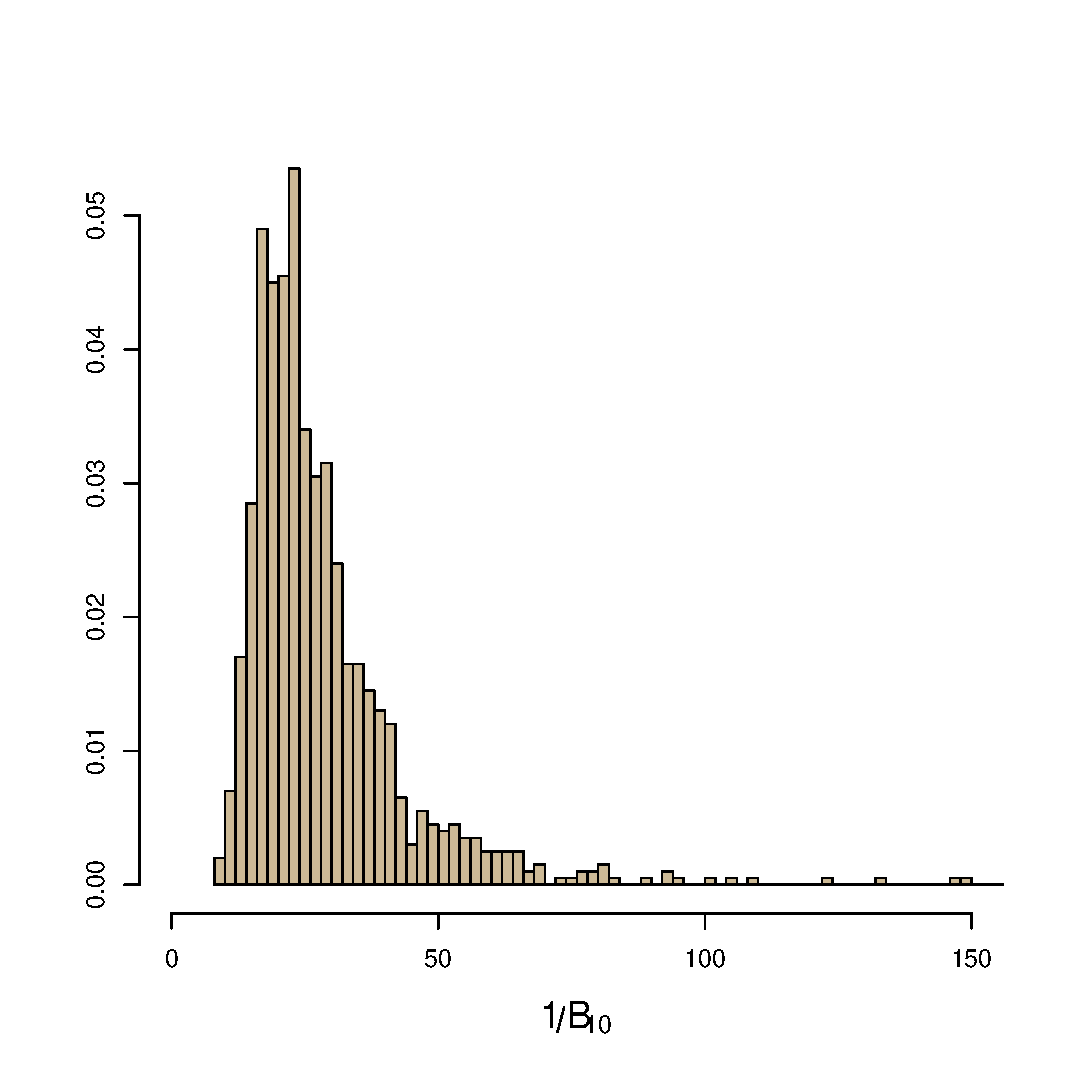
\includegraphics[height=3truecm]{figures/compbf}
\end{columns}
\end{block}

\end{slide}\begin{slide}
\debut[Cauchy-normal]
For estimating a normal mean, a 
{\it robust} prior is a Cauchy prior
$$
  x \sim \CN (\theta,1), \quad \theta \sim {\cal C}(0,1).
$$

Under squared error loss, posterior mean
$$
\delta^\pi(x)=\frac{\displaystyle{ \int_{-\infty}^{\infty} 
\frac{\theta}{1+\theta^2}} 
e^{-(x-\theta)^2/2} d\theta}{\displaystyle{\int_{-\infty}^{\infty} 
\frac{1}{1+\theta^2}} e^{-(x-\theta)^2/2} d\theta}
$$
\fin

\end{slide}\begin{slide}
\debut[Cauchy-normal (2)]
Form of $\delta^\pi$ suggests simulating iid variables 
$\theta_1, \cdots, \theta_m \sim \CN (x,1)$ and calculate
\begin{columns}\column{.48\textwidth}
\begin{displaymath}
 \hat{\delta}^\pi_m(x)=\frac{\sum_{i=1}^m 
\displaystyle{\frac{\theta_i}{1+\theta_i^2}}}{\sum_{i=1}^m 
\displaystyle{\frac{1}{1+\theta_i^2}}}  \;.
\end{displaymath}

\pause
LLN implies
$$\hat{\delta}^\pi_m(x) \longrightarrow 
\delta^\pi(x)\mbox{ as } m \longrightarrow \infty.$$ 
\column{.45\textwidth}
\includegraphics[height=\textwidth,width=5cm,angle=270]{figures/rangeofco.ps}
\end{columns}\fin

\end{slide}\begin{slide}
%\subsubsection{Importance Sampling}\label{sec:imosa}
\slidetitle{Importance sampling}

Simulation from $f$ (the true density) is not necessarily {\Red{\bf optimal}}

\medskip\pause
Alternative to direct sampling from $f$ is {\Emerald{\bf importance sampling}},
based on the alternative representation 
$$\Brown{
\BE_f[h(x)]  = \int_{\cal{X}} \; \left[ h(x) \; {f(x)\over g(x)} \right]\; g(x) \; dx
= \BE_g\left[ h(x)\frac{f(x)}{g(x)}\right]
}$$
which allows us to use \RawSienna{{\bf other}} distributions than $f$

\end{slide}\begin{slide}
\slidetitle{Importance sampling (cont'd)}
\begin{block}{Importance sampling algorithm}
Evaluation of
$$
  \BE_f[h(x)] = \int_{\CX} \; h(x) \; f(x) \; dx
$$
by 
{\sf \begin{enumerate}
\item Generate a sample $x_1,\ldots,x_m$ from a distribution $g$
\item Use the approximation
$$
 {1\over m}\; \sum_{j=1}^m\; {f(x_j)\over g(x_j)}\; h(x_j)
$$
\end{enumerate}
}\end{block}

\end{slide}\begin{slide}
\slidetitle{Justification}

Convergence of the estimator
$$
{1\over m}\; \sum_{j=1}^m\; {f(x_j)\over g(x_j)}\;h(x_j)
\longrightarrow  \BE_f[h(x)]
$$

\begin{enumerate}
\item converges for any choice
of the distribution $g$ as long as $\mathrm{ supp}(g) \supset \mathrm{ supp}(f)$

\pause
\item Instrumental distribution 
$g$ chosen from distributions easy to simulate

\pause
\item Same sample (generated from $g$) 
can be used repeatedly, not only for different functions 
$h$, but also for different densities $f$
\end{enumerate}

\end{slide}\begin{slide}
\slidetitle{Choice of importance function}
$g$ can be any density but some choices better than others

\begin{enumerate}
\item Finite variance only when 
$$
\BE_f \left[ h^2(x)  \frac{f(x)}{g(x)} \right] = \int_{\cal X}\; h^2(x)\; 
\frac{f^2(x)}{g(x)} \; dx < \infty \; .  
$$

\pause
\item Instrumental distributions with tails
lighter than those of $f$ (that is, with $\sup f/g = \infty$)
not appropriate, because weights $f(x_j)/g(x_j)$ vary widely,
giving too much importance to a few values $x_j$.

\pause
\item If $\sup f/g = M < \infty$, the accept-reject algorithm
can be used as well to simulate $f$ directly.

\pause
\item IS suffers from curse of dimensionality
\end{enumerate}


\end{slide}\begin{slide}
\debut[Cauchy target]
Case of Cauchy distribution $\mathcal{C}(0,1)$ when importance function is 
Gaussian $\mathscr{N}(0,1)$. 
\begin{columns}\column{.5\textwidth}
Density ratio 
$$
\frac{p^\star(x)}{p_0(x)}
= \sqrt{2\pi}\,\frac{\exp x^2/2}{\pi\,(1+x^2)}
$$
very badly behaved: e.g.,
$$
\int_{-\infty}^{\infty} \varrho(x)^2 p_0(x) dx = \infty
$$
\column{.45\textwidth}
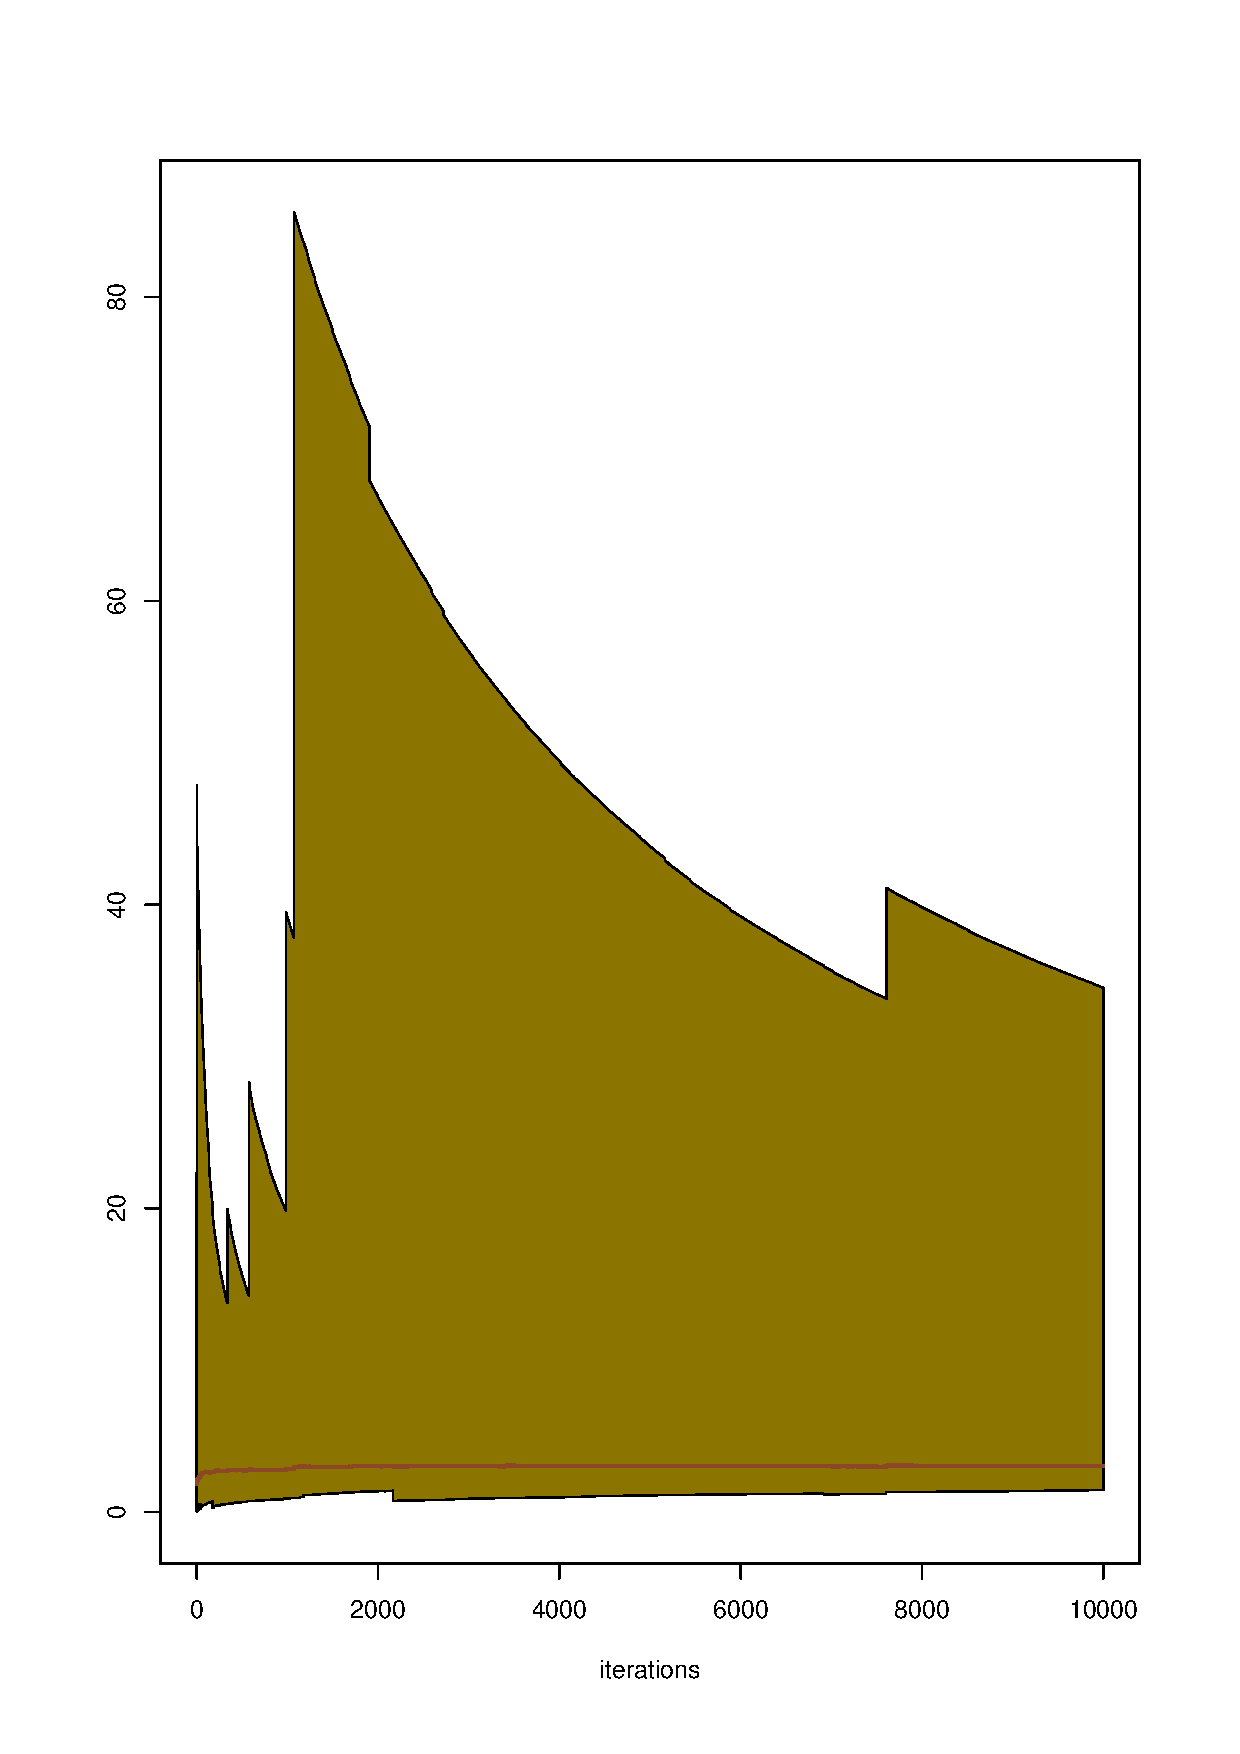
\includegraphics[height=3.5truecm,width=.9\textwidth]{figures/impinf}
\end{columns}

Poor performances of the
associated importance sampling estimator 
\fin

\end{slide}
\begin{slide}
\slidetitle{Practical alternative}
\begin{displaymath}
\sum_{j=1}^m \; h(x_{j}) \; f(x_{j}) / g(x_{j}) \bigg/
\sum_{j=1}^m \; f(x_{j}) / g(x_{j})
\end{displaymath}
where $f$ and $g$ are known up to constants.

\begin{enumerate}
\item Also converges to ${\mathfrak{I}}$ by the Strong Law of Large Numbers.
\item Biased, but the bias is quite small:
may beat the unbiased estimator in squared error loss.
\end{enumerate}  

\end{slide}\begin{slide}
\debut[Student's $t$ distribution]
$x \sim {\cal{T}}(\nu,\theta,\sigma^2)$, with density
$$
f_\nu(x) = {\Gamma((\nu+1)/2)\over \sigma \sqrt{\nu\pi} \; \Gamma(\nu/2)}
\left(1+{(x - \theta)^2\over \nu \sigma^2}\right)^{-(\nu+1)/2} \;. 
$$

Without loss of generality, take $\theta = 0$, $\sigma = 1$.

\pause
Integral of interest
$$
\mathfrak{I} = \int \sqrt{\left|{x\over 1-x}\right|} \,f_\nu(x) \,\hbox{d}x
$$
\fin

\end{slide}\begin{slide}
\debut[Student's $t$ distribution (2)]
\begin{columns}\column{.45\textwidth}
Choices of h:
\begin{enumerate}
\item Student \ \Brown{${\mathcal{T}}(\nu,0,1)$}  
\item Cauchy \ \Brown{${\mathcal{C}}(0,1)$}       
\item Normal \ \Brown{$\mathscr{N}(0,\nu/(\nu-2))$}   
\end{enumerate}

{\bf Note:} The ratio
$$\Red{
{f^2(x) \over h(x) } \propto
{e^{x^2(\nu-2)/2\nu}\over [1 + x^2/\nu]^{(\nu+1)}}
}$$
does not have a finite integral
\column{.5\textwidth}
\includegraphics[width=5cm,height=\textwidth,angle=270]{figures/student.range.eps} 
\end{columns}
\fin

\end{slide}\begin{slide}
\slidetitle{Explanation}
\debut[Student's $t$ distribution (3)]
Phenomenon due to the fact that $h$ has a singularity at $x=1$:
$$
\int \frac{|x|}{|1-x|} f_\nu(x) \,\hbox{d}x = \infty
$$

\pause
\Sepia{{\bf Consequence:} the three estimators have infinite variance}
\fin

\end{slide}\begin{slide}
\slidetitle{Alternative} 
\debut[Student's $t$ distribution (4)]
Choose a better behaved $h$: \pause
folded Gamma distribution, $x$ symmetric around $1$ with
\begin{columns}\column{.55\textwidth}
$$
|x-1| \sim\mathcal{G}a(\alpha,1)
$$ 
Then  $h_1(x)f^2(x)/h(x)$ proportional to
$$
\sqrt{x}\,f^2(x)\,|1-x|^{1-\alpha-1}\,\exp|1-x|
$$
integrable around $x=1$ when $\alpha<1$.
\column{.42\textwidth}
\includegraphics[width=4cm,height=\textwidth,angle=270]{figures/student.best.eps}
\end{columns}
\fin

\end{slide}\begin{slide}
\slidetitle{Choice of importance function (termin'd)}
{\BurntOrange{\fbox{\bf The importance function may be $\pi$}}}

\medskip\pause
\begin{itemize}
       \item  often inefficient if data informative
       \item  impossible if $\pi$ is improper
\end{itemize}

\pause\medskip
{\BurntOrange{\fbox{\bf Defensive sampling:}}}
$$
h(\theta) = \rho \pi(\theta) + (1-\rho) \pi(\theta|x) \qquad \rho\ll 1
$$
\end{slide}\begin{slide}
\debut[Cauchy/Normal] \ Consider
$$
  	x_1,\ldots,x_n \sim \CC(\theta,1)
\qquad \text{and} \qquad
	\theta\sim\CN(\mu,\sigma^2),
$$
with known \hypa s $\mu$ and $\sigma^2$.

\pause
Since $\pi(\theta)$ is normal $\CN(\mu, \sigma^2)$, possible 
to simulate a normal sample $\theta_1,\ldots,\allowbreak\theta_M$ 
and to approximate the Bayes estimator by
\[
\hat\delta^\pi(x_1,\ldots,x_n) =
{\sum_{t=1}^M \theta_t \prod_{i=1}^n [1+(x_i-\theta_t)^2]^{-1} \over 
\sum_{t=1}^M \prod_{i=1}^n [1+(x_i-\theta_t)^2]^{-1}}.
\]
\fin

\end{slide}\begin{slide}
\debut[Cauchy/Normal (2)]

Poor when the $x_i$'s are all far from $\mu$

\centerline{\includegraphics[height=10cm,angle=270,width=5cm]{figures/fig622.ps}}
$90\%$ range of variation 
for $n=10$ observations from $\CC (0,1)$ distribution and $M=1000$
simulations of $\theta$ as $\mu$ varies
\fin

\end{slide}\begin{slide}
\slidetitle{Bridge sampling}
Bayes factor
$$
B^\pi_{12} = { \displaystyle{\int f_1(x|\theta_1) \pi_1(\theta_1) d\theta_1} \over
\displaystyle{\int f_2(x|\theta_2) \pi_2(\theta_2) d\theta_2} }
$$

\pause
If
$$
\begin{array}{lll}
\pi_1(\theta_1|x) &\propto& {\tilde\pi}_1(\theta_1|x) \\
\pi_2(\theta_2|x) &\propto& {\tilde\pi}_2(\theta_2|x) 
\end{array}          
$$
then
$$
B^\pi_{12} \approx {1\over n} \sum_{i=1}^n { {\tilde\pi}_1(\theta_i|x) \over
            {\tilde\pi}_2(\theta_i|x) }  \hspace{1cm}  \theta_i \sim \pi_2(\theta|x)
$$

\end{slide}
\subsection{Prediction}
\begin{slide}\slidetitle{Prediction}

If $x \sim f(x|\theta)$ and $z\sim g(z|x,\theta)$, 
the {\it predictive} of $z$ is
\[{\Brown{
 g^\pi(z|x) = \int_{\Theta} g(z|x,\theta)\pi(\theta|x)\,d\theta.
}}\]

\end{slide}\begin{slide}\slidetitle{Normal prediction}

For $\mathscr{D}_n=(x_1,\ldots,x_n)\sim\mathscr{N} (\mu,\sigma^2)$ and
$$
\pi(\mu,\sigma^2) \propto (\sigma^2)^{-\lambda_\sigma-3/2}\,
	\exp-\left\{ -\lambda_\mu(\mu-\xi)^2 + \alpha\right\}/2\sigma^2\,,
$$
corresponding posterior 
\footnotesize
$$
\mathscr{N}\left(\frac{\lambda_\mu\xi+n\overline x_n}{\lambda_\mu+n},
\frac{\sigma^2}{\lambda_\mu+n}\right) \times \mathscr{IG} \left(
\lambda_\sigma+n/2,\left[
\alpha+s^2_x+\frac{n\lambda_\mu}{\lambda_\mu+n}(\overline x - \xi)^2\right]/2 \right)\,,
$$
\normalsize

\pause \BurntOrange{{\bf Notation}}
$$
\mathscr{N}\left(\xi(\mathscr{D}_n),\sigma^2/\lambda_\mu(\mathscr{D}_n)
\right) \times \mathscr{IG} \left(
\lambda_\sigma(\mathscr{D}_n),\alpha(\mathscr{D}_n)/2 \right)
$$

\end{slide}\begin{slide}\slidetitle{Normal prediction (cont'd)}

Predictive on $x_{n+1}$
\small 
\begin{align*}
f^\pi(x_{n+1}|\mathscr{D}_n) &\propto \int (\sigma^2)^{-\lambda_\sigma-2-n/2}\,
\exp-(x_{n+1}-\mu)^2/2\sigma^2 \\
&\qquad \times \exp-\left\{ \lambda_\mu(\mathscr{D}_n)(\mu-\xi(\mathscr{D}_n))^2
+ \alpha(\mathscr{D}_n) \right\}/2\sigma^2\,\hbox{d}(\mu,\sigma^2)\\
&\propto \int (\sigma^2)^{-\lambda_\sigma-n/2-3/2}\,
\exp-\left\{ (\lambda_\mu(\mathscr{D}_n)+1)(x_{n+1}-\xi(\mathscr{D}_n))^2\right.\\
&\qquad\left.
/\lambda_\mu(\mathscr{D}_n) +\alpha(\mathscr{D}_n) \right\}/2\sigma^2\,\hbox{d}\sigma^2\\
&\propto \left[ \alpha(\mathscr{D}_n) + \frac{\lambda_\mu(\mathscr{D}_n)+1}{
\lambda_\mu(\mathscr{D}_n)} (x_{n+1}-\xi(\mathscr{D}_n))^2 \right]^{-(2\lambda_\sigma+n+1)/2}
\end{align*}
\normalsize
Student's $t$ distribution with mean $\xi(\mathscr{D}_n)$ 
and $2\lambda_\sigma+n$ degrees of freedom.


\end{slide}\begin{slide}\slidetitle{{\sf normaldata}}

Noninformative case $\lambda_\mu=\lambda_\sigma=\alpha=0$ 
$$
f^\pi(x_{n+1}|\mathscr{D}_n)\propto
\left[s_x^2+\frac{n}{n+1}(x_{n+1}-\overline x_n)^2\right]^{-(n+1)/2}\,.
$$

\begin{columns}
\column{.48\textwidth}
Predictive distribution on a $91$st county 
is Student's $t$ 
$$
\mathscr{T}(90,-0.0413,0.136)
$$
\column{.5\textwidth}
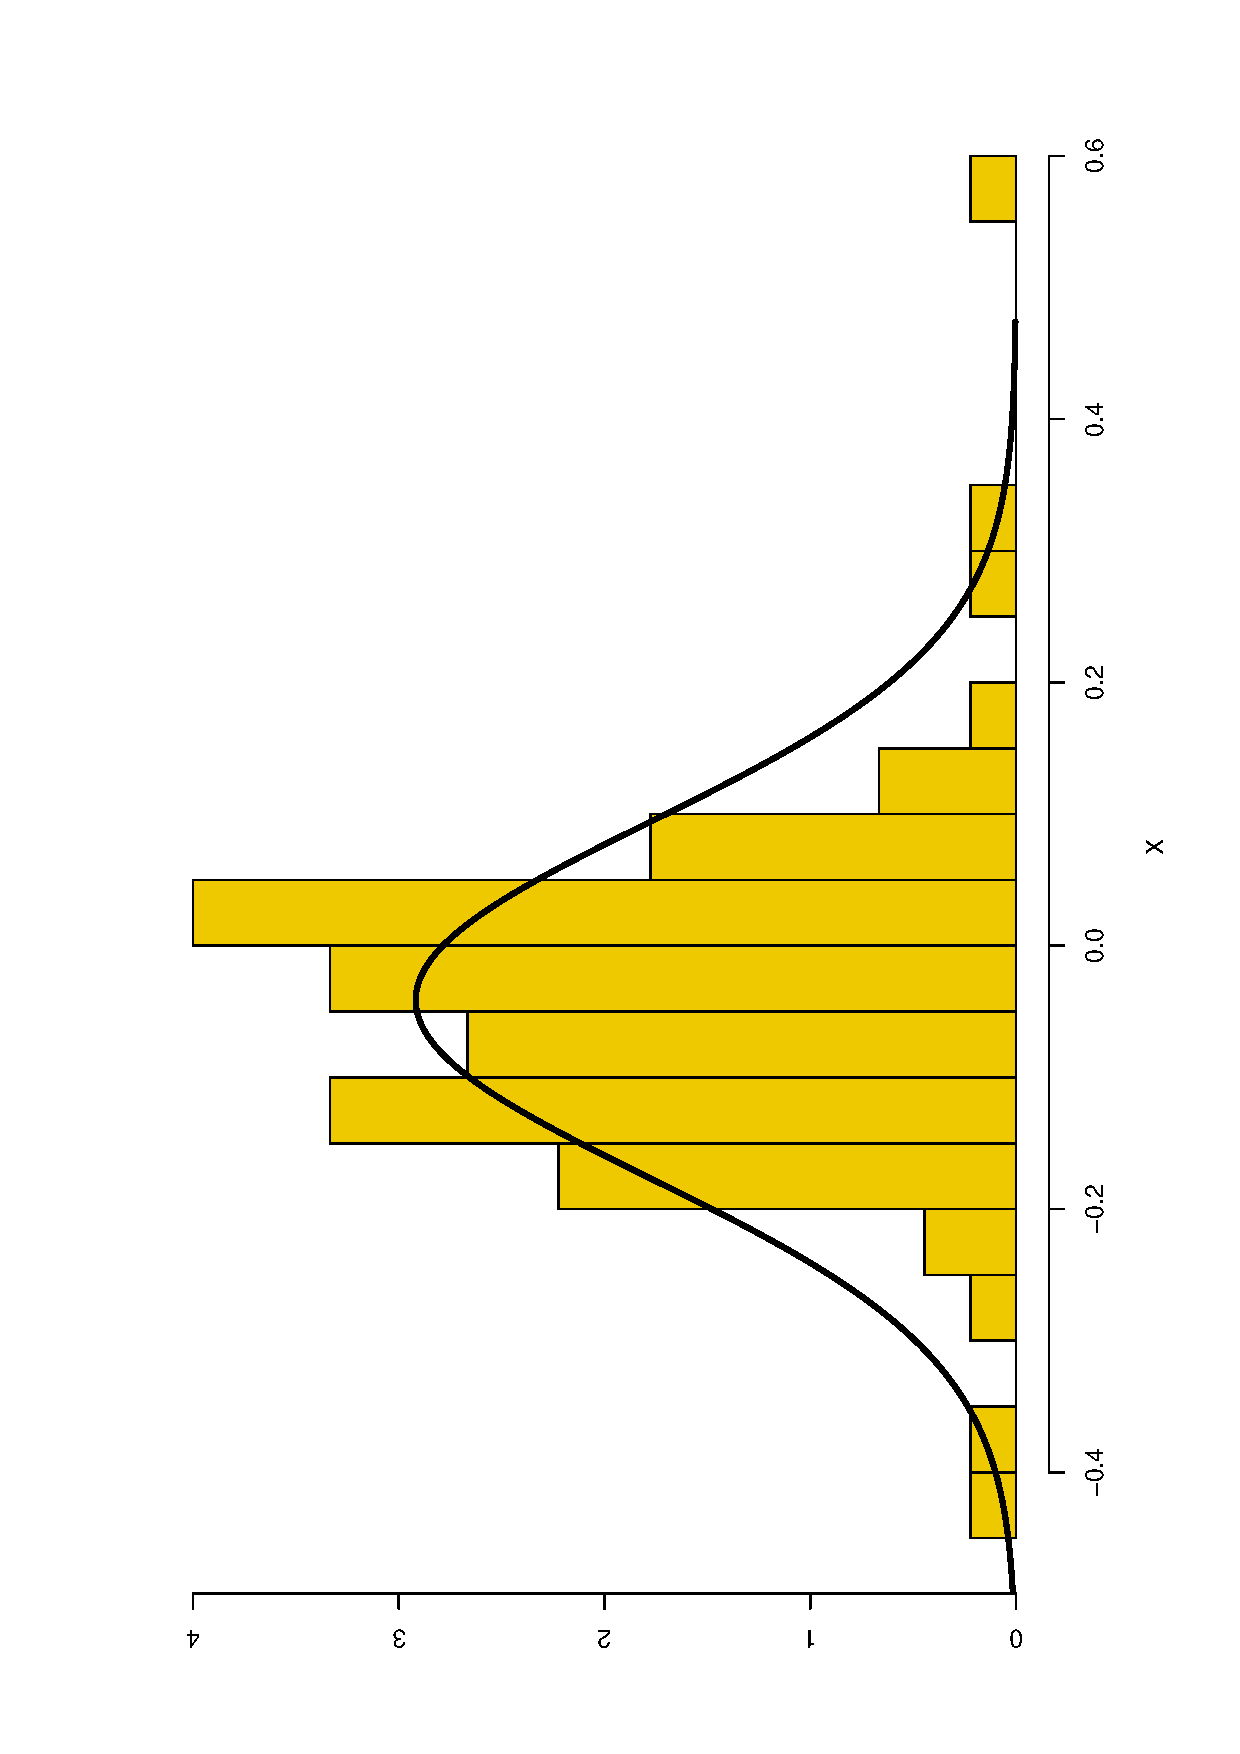
\includegraphics[width=4truecm,angle=270]{figures/predt}
\end{columns}
\end{slide}

\section{Regression and variable selection}
\begin{slide}\slidetitle{Regression and variable selection}
\tableofcontents[sectionstyle=show/hide,subsectionstyle=show/shaded/hide]

\end{slide}
\subsection{Regression}\begin{slide}\slidetitle{Regression}

Large fraction of statistical analyses dealing with representation of dependences between several 
variables, rather than marginal distribution of each variable

\end{slide}\begin{slide}\slidetitle{Pine processionary caterpillars}

\begin{columns}
\column{.45\textwidth}
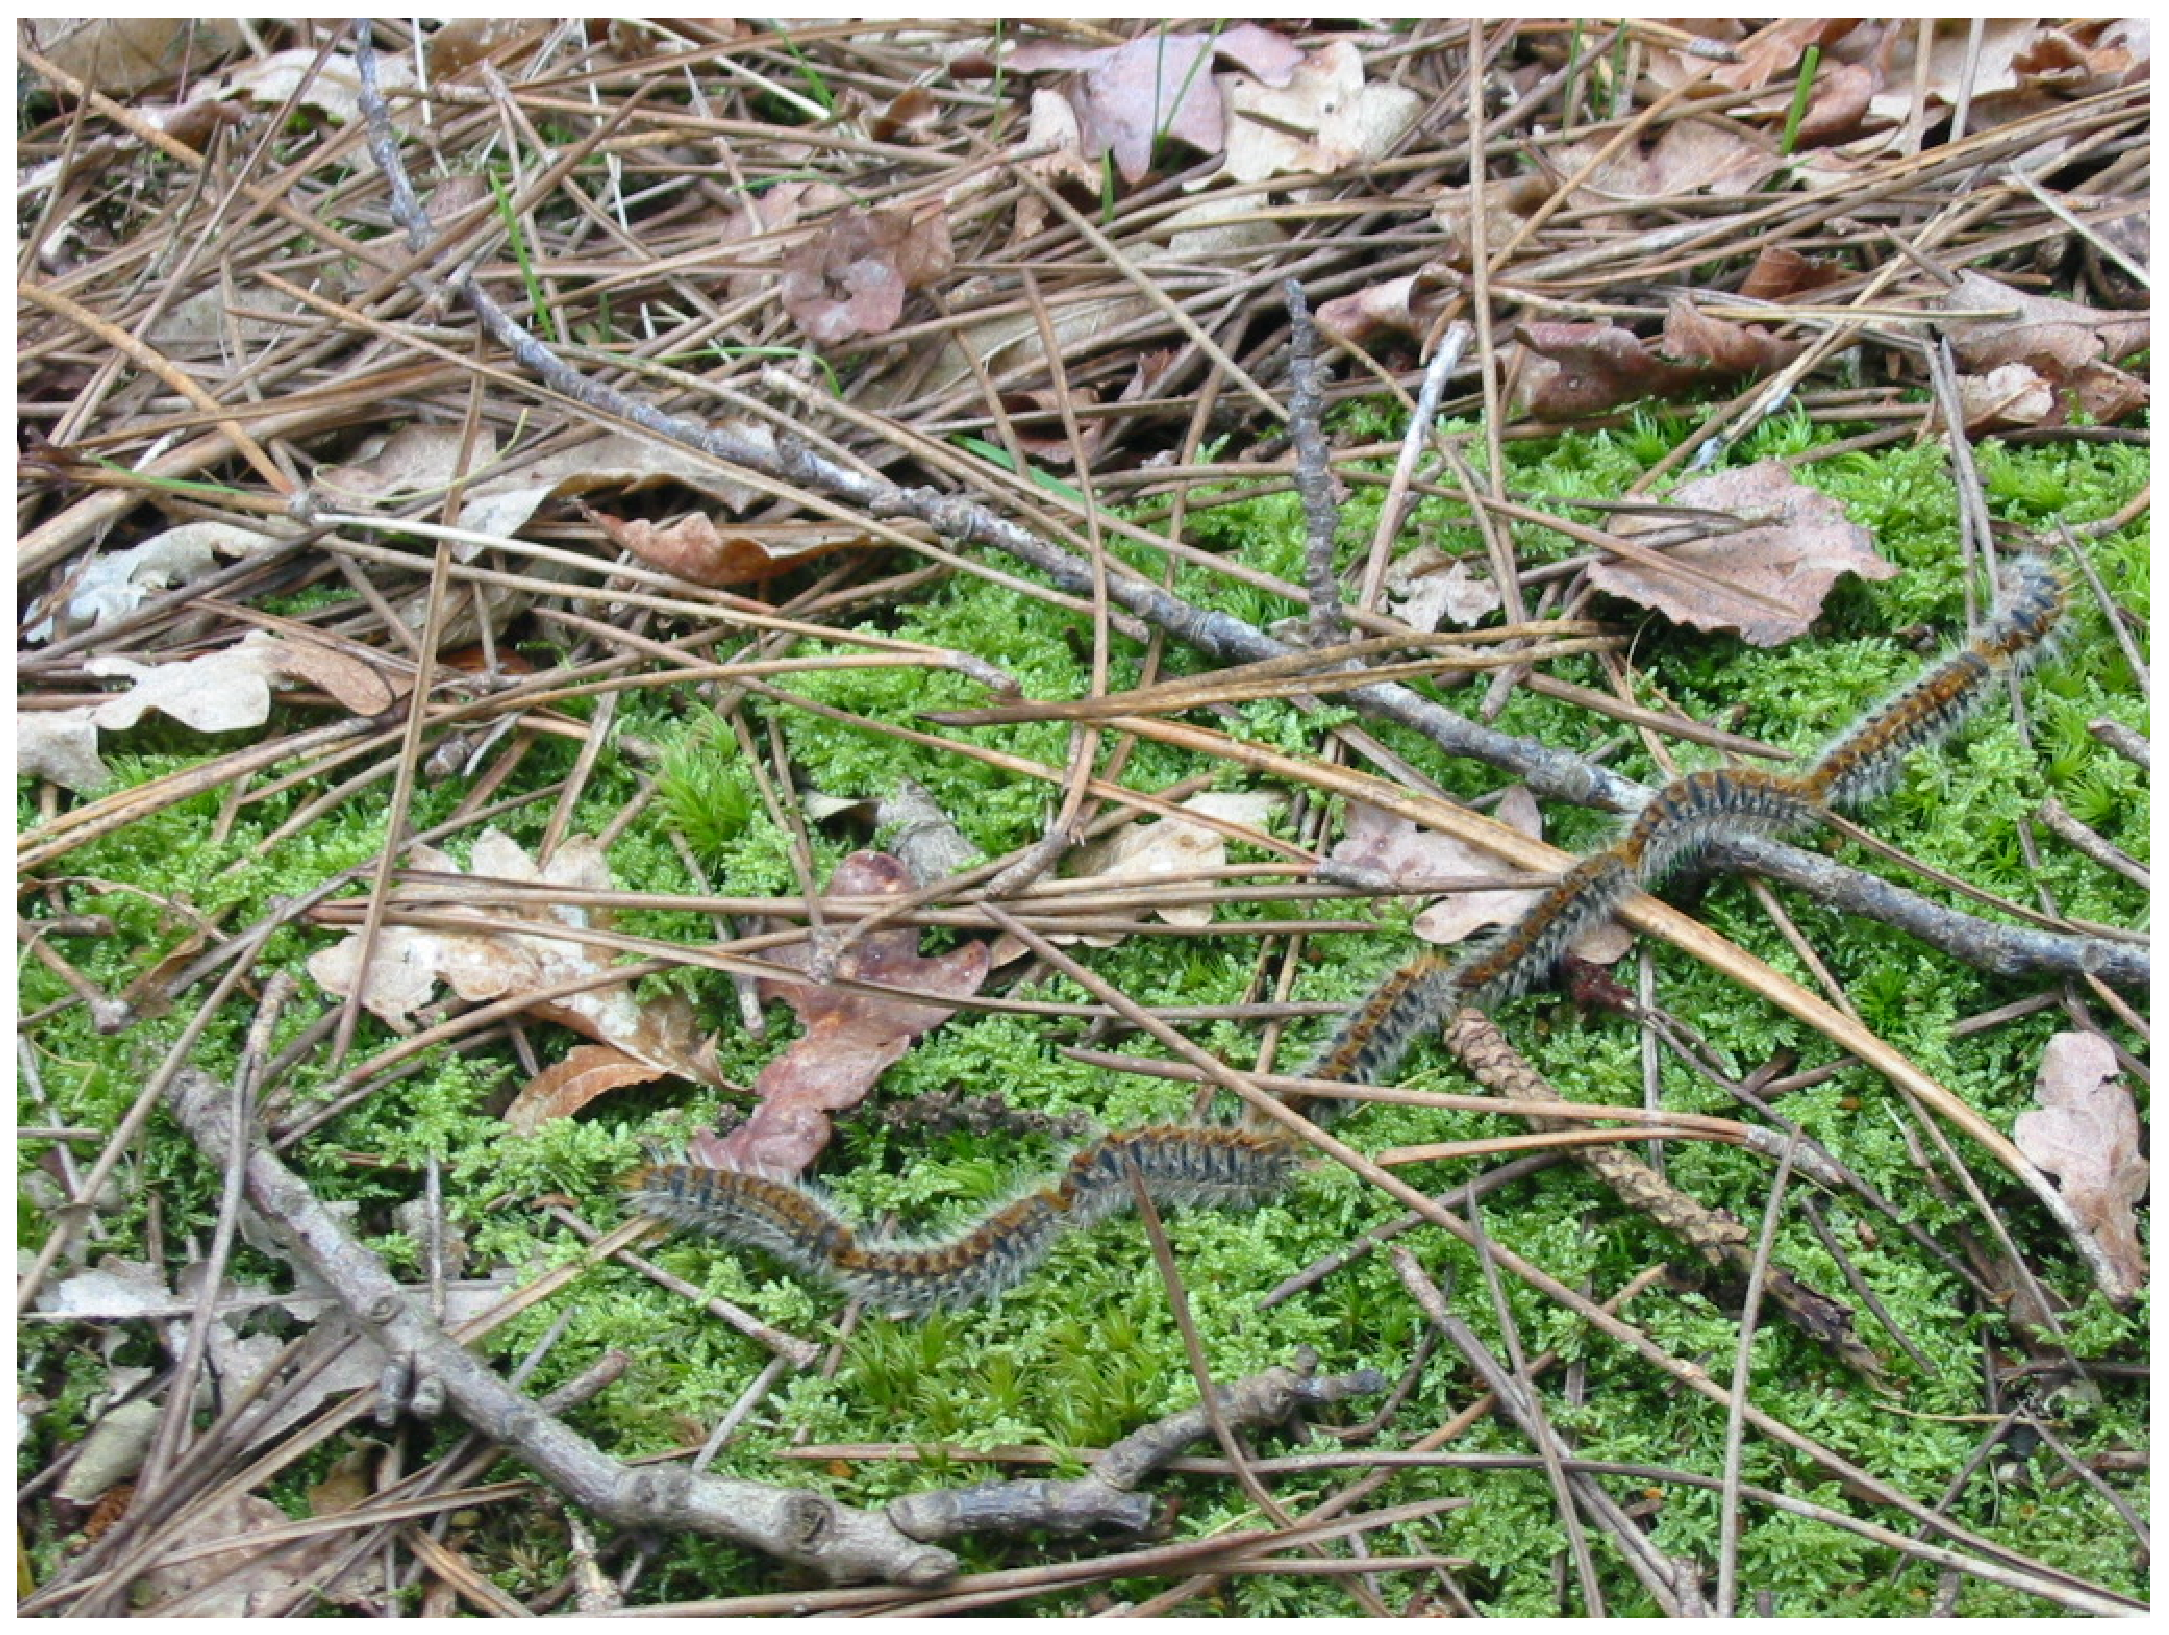
\includegraphics[width=5cm]{figures/caterpibreizh.eps}
\pause
\column{.45\textwidth}
\only<2>{Pine processionary caterpillar colony size influenced by
\tiny
\begin{itemize}
\item[] $x_1$ altitude
\item[] $x_2$ slope (in degrees)
\item[] $x_3$ number of pines in the area
\item[] $x_4$ height of the central tree
\item[] $x_5$ diameter of the central tree
\item[] $x_6$ index of the settlement density
\item[] $x_7$ orientation of the area (from $1$ [southbound] to $2$)
\item[] $x_8$ height of the dominant tree
\item[] $x_9$ number of vegetation strata
\item[] $x_{10}$ mix settlement index (from $1$ if not mixed to $2$ if mixed)
\end{itemize}
\normalsize}
\only<3>{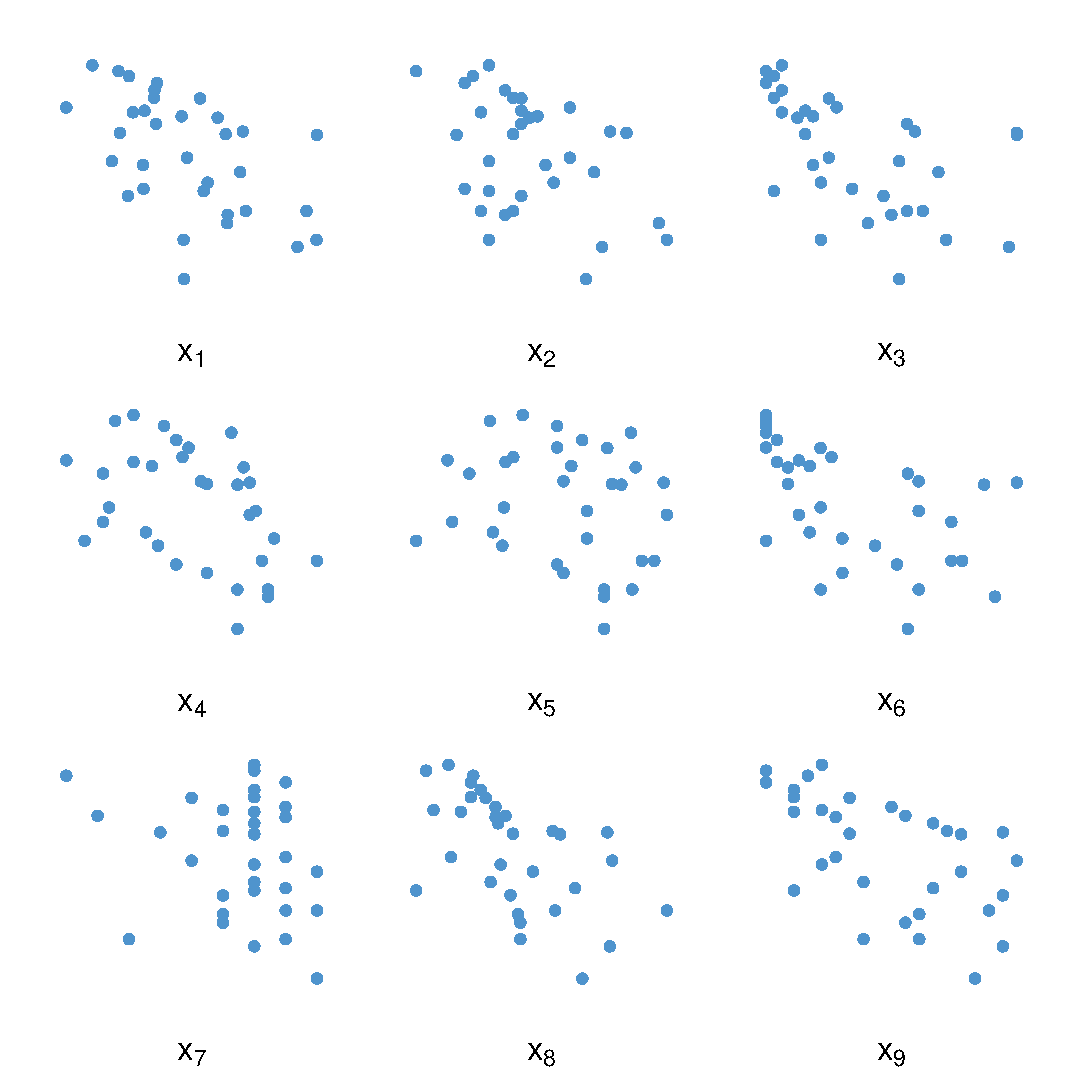
\includegraphics[width=5cm]{figures/processimpl.eps}}
\end{columns}

\end{slide}\begin{slide}\slidetitle{Goal of a regression model}

From a statistical point of view, find a proper representation
of the distribution, $f(y|\theta,x)$, of an observable variable $y$ 
given a vector of observables $x$, based on a sample of $(x,y)_i$'s. 

\end{slide}\begin{slide}\slidetitle{Linear regression}

Linear regression: one of the most widespread tools of Statistics for analysing (linear) influence 
of some variables or some factors on others

\vs\pause
\begin{block}{Aim}{\centerline{\BurntOrange{To uncover explanatory and predictive patterns}}}\end{block}

\end{slide}\begin{slide}\slidetitle{Regressors and response}

Variable of primary interest, $y$, called the \textit{response} or the \textit{outcome} variable
[assumed here to be continuous]

\begin{flushright}E.g., number of Pine processionary caterpillar colonies\end{flushright}

\pause
Covariates $x=(x_1,\ldots,x_k)$ called \textit{explanatory variables} [may be discrete, 
continuous or both]

\pause
\vs Distribution of $y$ given $x$ typically studied in the context of a set of \textit{units} or
experimental \textit{subjects},  $i=1,\ldots,n$, for instance patients in an hospital ward,
on which both $y_i$ and $x_{i1},\ldots,x_{ik}$ are measured.

\end{slide}\begin{slide}\slidetitle{Regressors and response cont'd}

Dataset made of the conjunction of the vector of outcomes
$$
y=\left(y_1,\ldots,y_n\right)
$$ 
\pause
and of the $n\times (k+1)$ matrix of explanatory variables
$$
X=\left[\begin{array}{ccccc}
 1      & x_{11} & x_{12} & \ldots & x_{1k} \\
 1      & x_{21} & x_{22} & \ldots & x_{2k} \\
 1      & x_{31} & x_{32} & \ldots & x_{3k} \\
 \vdots & \vdots & \vdots & \vdots & \vdots \\
 1      & x_{n1} & x_{n2} & \ldots & x_{nk}
\end{array}\right]
$$

\end{slide}\subsection{Linear models}
\begin{slide}\slidetitle{Linear models}

\textit{Ordinary normal linear regression} model such that
$$
y|\beta,\sigma^2,X\sim\mathscr{N}_n(X\beta,\sigma^2I_n)
$$
\pause
and thus
\begin{eqnarray*}
\mathbb{E}[y_i|\beta,X]    &=& \beta_0+\beta_1x_{i1}+\ldots+\beta_kx_{ik}\\
\mathbb{V}(y_i|\sigma^2,X) &=& \sigma^2
\end{eqnarray*}

\end{slide}\begin{slide}\slidetitle{Categorical variables}

\begin{itemize}
\item[{\Large $\lightning$}]
There \BrickRed{is} a difference between finite valued regressors like $x_7$ in {\sf caterpillar} 
\Brown{[orientation of the area]} and
{\em categorical} variables (or {\em factors}), which are also taking a finite number of values
but whose range has no numerical meaning.
\end{itemize}

\pause
\begin{example}
If $x$ is the socio-professional category of an employee, this variable ranges from $1$ to $9$ 
for a rough grid of socio-professional activities, and from $1$ to $89$ on a finer grid. 

\BurntOrange{\centerline{The numerical values are not comparable}}
\end{example}

\end{slide}\begin{slide}\slidetitle{Categorical variables (cont'd)}

Makes little sense to involve $x$ directly in the regression: replace the single regressor $x$ [in
$\{1,\ldots,m\}$, say] with $m$ indicator (or {\em dummy}) variables 
$$
x_1=\mathbb{I}_1(x), \ldots, x_m=\mathbb{I}_m(x)
$$

\pause
\begin{block}{\BrickRed{Convention}}
Use of a different constant $\beta_i$ for each class categorical variable value:
$$
\mathbb{E}[y_i|\beta,X] = \ldots + \beta_1\mathbb{I}_1(x)+\ldots+\beta_m\mathbb{I}_m(x)+\ldots
$$
\end{block}

\end{slide}\begin{slide}
\slidetitle{Identifiability}

Identifiability issue: For dummy variables, sum of the indicators equal to one.


\begin{block}{Convention}
Assume that $X$ is of full rank:
$$\BrickRed{
\mbox{rank}(X)=k+1
}$$
[$X$ is of full rank if and only if $X^\tee X$ is invertible]
\end{block}

\pause
\begin{flushright} E.g., for dummy variables, this means eliminating one class \end{flushright}

\end{slide}\begin{slide}
\slidetitle{Likelihood function \&\ estimator}

The likelihood of the \textit{ordinary normal linear model} is
$$
\ell\left(\beta,\sigma^2|y,X\right)=\left(2\pi\sigma^2\right)^{-n/2}\,
\exp\left[-\frac{1}{2\sigma^2}(y-X\beta)^\tee (y-X\beta)\right]
$$

\pause\vs The MLE of $\beta$ is solution of the least squares minimisation problem
\small
$$
\min_\beta\, (y-X\beta)^\tee (y-X\beta) = \min_\beta
\,\sum_{i=1}^n\left(y_i-\beta_0-\beta_1x_{i1}-\ldots-\beta_kx_{ik}\right)^2\,,
$$
\normalsize
namely
$$\BrickRed{
\hat\beta=(X^\tee X)^{-1}X^\tee y
}$$

\end{slide}\begin{slide}
\slidetitle{Least square estimator}
\begin{itemize}
\item $\hat\beta$ is an unbiased estimator of $\beta$.

\item $\mathbb{V}(\hat\beta|\sigma^2,X)=\sigma^2(X^\tee X)^{-1}$

\item $\hat\beta$ is the {\em best} linear unbiased estimator of $\beta$: 
for all $a\in\mathbb{R}^{k+1}$, 
$$
\mathbb{V}(a^\tee\hat\beta|\sigma^2,X)\leq\mathbb{V} (a^\tee\tilde\beta|\sigma^2,X)
$$
for any unbiased linear estimator $\tilde\beta$ of $\beta$.

\item Unbiased estimator of $\sigma^2$
$$
\hat\sigma^2=\frac{1}{n-k-1}(y-X\hat\beta)^\tee (y-X\hat\beta)=\frac{s^2}{n-k-1},
$$
\end{itemize}

\end{slide}
\begin{frame}[fragile]
\frametitle{Pine processionary caterpillars}

\footnotesize
\begin{verbatim}
Residuals:        Min       1Q     Median     3Q        Max
                -1.6989  -0.2731   -0.0003  0.3246     1.7305
Coefficients:
             Estimate Std. Error t value Pr(>|t|)
intercept   10.998412   3.060272   3.594  0.00161 **
XV1         -0.004431   0.001557  -2.846  0.00939 **
XV2         -0.053830   0.021900  -2.458  0.02232 * 
XV3          0.067939   0.099472   0.683  0.50174
XV4         -1.293636   0.563811  -2.294  0.03168 *
XV5          0.231637   0.104378   2.219  0.03709 *
XV6         -0.356800   1.566464  -0.228  0.82193
XV7         -0.237469   1.006006  -0.236  0.81558
XV8          0.181060   0.236724   0.765  0.45248
XV9         -1.285316   0.864847  -1.486  0.15142
XV10        -0.433106   0.734869  -0.589  0.56162
---
Signif. codes:  
0 `***' 0.001 `**' 0.01 `*' 0.05 `.' 0.1 ` ' 1
\end{verbatim}
\normalsize

\end{frame}
\subsection{Zellner's informative $G$-prior}
%\newcommand\by{\mathbf{y}}
\begin{slide}\slidetitle{Conjugate priors}

If [conditional prior] 
$$
\beta|\sigma^2,X\sim\mathscr{N}_{k+1}(\tilde\beta,\sigma^2M^{-1})\,,
$$
where $M$ $(k+1,k+1)$ positive definite symmetric matrix, and 
$$
\sigma^2|X\sim \mathscr{IG}(a,b),\qquad a,b>0,
$$
\pause then
\small
$$
\beta|\sigma^2,\by,X\sim
\mathscr{N}_{k+1}\left((M+X^\tee X)^{-1}
\{(X^\tee X)\hat\beta+M\tilde\beta\},\sigma^2(M+X^\tee X)^{-1}\right)
$$
and 
$$
\sigma^2|\by,X\sim
\mathscr{IG}\left(\frac{n}{2}+a,b+\frac{s^2}{2}+\frac{(\tilde\beta-\hat\beta)^\tee
\left(M^{-1}+(X^\tee X)^{-1}\right)^{-1}(\tilde\beta-\hat\beta)}{2}\right)
$$
\normalsize

\end{slide}
\begin{slide}\slidetitle{Experimenter dilemma}

Problem of the choice of $M$ or of $c$ if $M=I_{k+1}/c$

\pause
\begin{example}[Processionary caterpillar]
No precise prior information about $\tilde\beta$, $M$, $a$ and $b$. Take
$a=2.1$ and $b=2$, i.e.~prior mean and prior variance of $\sigma^2$ equal to
$1.82$ and $33.06$, and $\tilde\beta=0_{k+1}$.

\pause
Lasting influence of $c$: 
\small
\begin{center}\begin{tabular}{r r r r}
        $c$ &  $\ \mathbb{E}^\pi(\sigma^2|\by,X)$ & $\ \mathbb{E}^\pi(\beta_0|\by,X)$ & $\ \mathbb{V}^\pi(\beta_0|\by,X)$ \\
    \hline
   .1 &  1.0044 &  0.1251 & 0.0988 \\
   1   &  0.8541 &  0.9031 & 0.7733 \\
  10   &  0.6976 &  4.7299 & 3.8991 \\
 100   &  0.5746 &  9.6626 & 6.8355 \\
1000   &  0.5470 & 10.8476 & 7.3419
\end{tabular}\end{center}
\normalsize
\end{example}

\end{slide}
\begin{slide}\slidetitle{Zellner's informative $G$-prior}

\begin{block}{Constraint}
Allow the experimenter to 
introduce information about the location parameter of the regression 
while bypassing the most difficult aspects of the prior specification, 
namely the derivation of the prior correlation structure. 
\end{block}

\pause
\vs Zellner's prior corresponds to
\begin{eqnarray*}\BrickRed{
\beta|\sigma^2,X &\sim& \mathscr{N}_{k+1}(\tilde\beta,c\sigma^2(X^\tee X)^{-1})\\
\sigma^2 &\sim& \pi(\sigma^2|X)\propto\sigma^{-2}\,.
}\end{eqnarray*}
\emfarite{Special conjugate}

\end{slide}\begin{slide}
\slidetitle{Prior selection}

Experimental prior determination restricted to the choices of $\tilde\beta$ and of the constant $c$. 

\medskip\begin{block}{Note} 
$c$ can be interpreted as a measure of the amount of information available in the prior 
relative to the sample. For instance, setting $1/c=0.5$ gives the prior the same weight 
as 50\% of the sample.
\end{block}

\pause
\begin{itemize}
\item[{\Large $\lightning$}]
There still \BrickRed{is} a lasting influence of the factor $c$
\end{itemize}

\end{slide}\begin{slide}
\slidetitle{Posterior structure}
With this prior model, the posterior simplifies into
\small
\begin{eqnarray*}
\pi(\beta,\sigma^2|y,X) & \propto & f(y|\beta,\sigma^2,X)\pi(\beta,\sigma^2|X) \\
&\propto& \left(\sigma^2\right)^{-(n/2+1)}\exp\left[-\frac{1}{2\sigma^2}(y-X\hat\beta)^\tee 
   (y-X\hat\beta)\right.\\
&&\quad \left.-\frac{1}{2\sigma^2}(\beta-\hat\beta)^\tee X^\tee X(\beta-\hat\beta)\right]
	\left(\sigma^2\right)^{-k/2}\\
&&\quad\times \exp\left[-\frac{1}{2c\sigma^2}(\beta-\tilde\beta)X^\tee X(\beta-\tilde\beta)\right]\,,
\end{eqnarray*}
\normalsize
because $X^\tee X$ used in both prior and likelihood 
\emfarite{$G$-prior trick}

\end{slide}\begin{slide}
\slidetitle{Posterior structure (cont'd)}
Therefore,
\begin{eqnarray*}
\beta|\sigma^2,y,X&\sim&\mathscr{N}_{k+1}\left(\frac{c}{c+1}(\tilde\beta/c+\hat\beta),
\frac{\sigma^2c}{c+1}(X^\tee X)^{-1}\right)\\
\sigma^2|y,X&\sim&\mathcal{IG}\left(\frac{n}{2},\frac{s^2}{2}+\frac{1}{2(c+1)}
(\tilde\beta-\hat\beta)^\tee X^\tee X(\tilde\beta-\hat\beta)\right)
\end{eqnarray*}
and
\small
\begin{eqnarray*}
\beta|y,X &\sim& \mathscr{T}_{k+1}\left(n,\frac{c}{c+1}\left(\frac{\tilde\beta}{c}+\hat\beta\right),\right. \\
&& \left.\frac{c(s^2+(\tilde\beta-\hat\beta)^\tee X^\tee 
X(\tilde\beta-\hat\beta)/(c+1))}{n(c+1)}(X^\tee X)^{-1}\right).
\end{eqnarray*}
\normalsize

\end{slide}\begin{slide}\slidetitle{Bayes estimator}

The Bayes estimators of $\beta$ and $\sigma^2$ are given by
$$
\mathbb{E}^\pi[\beta|y,X]=\frac{1}{c+1}(\tilde\beta+c\hat\beta)
$$
and
$$
\mathbb{E}^\pi[\sigma^2|y,X]=\frac{s^2+(\tilde\beta-\hat\beta)^\tee X^\tee X(\tilde\beta-\hat\beta)/(c+1)}{n-2}\,.
$$ 

\medskip\pause
{\bf Note:}
Only when $c$ goes to infinity does the influence of the prior vanish!

\end{slide}\begin{slide}
\slidetitle{Pine processionary caterpillars}

\only<1>{\begin{center}
\begin{tabular}{c|r r}
$\beta_i$ & $\ \mathbb{E}^\pi(\beta_i|\by,X)\ $ & $\ \mathbb{V}^\pi(\beta_i|\by,X)$ \\
 \hline $\beta_0$ & 10.8895 & 6.4094 \\
 $\beta_1$ & -0.0044 & 2e-06 \\
 $\beta_2$ & -0.0533 & 0.0003 \\
 $\beta_3$ &  0.0673 & 0.0068 \\
 $\beta_4$ & -1.2808 & 0.2175 \\
 $\beta_5$ &  0.2293 & 0.0075 \\
 $\beta_6$ & -0.3532 & 1.6793 \\
 $\beta_7$ & -0.2351 & 0.6926 \\
 $\beta_8$ &  0.1793 & 0.0383 \\
 $\beta_9$ & -1.2726 & 0.5119 \\
 $\beta_{10}$ & -0.4288 & 0.3696
\end{tabular}

		$c=100$
\end{center}}

\end{slide}\begin{slide}
\slidetitle{Pine processionary caterpillars (2)}
\only<1>{
\begin{center}
\begin{tabular}{c|r r}
$\beta_i$ & $\ \mathbb{E}^\pi(\beta_i|\by,X)\ $ & $\ \mathbb{V}^\pi(\beta_i|\by,X)$ \\
 \hline $\beta_0$ & 10.9874 & 6.2604 \\
 $\beta_1$ & -0.0044 & 2e-06 \\
 $\beta_2$ & -0.0538 & 0.0003 \\
 $\beta_3$ &  0.0679 & 0.0066 \\
 $\beta_4$ & -1.2923 & 0.2125 \\
 $\beta_5$ &  0.2314 & 0.0073 \\
 $\beta_6$ & -0.3564 & 1.6403 \\
 $\beta_7$ & -0.2372 & 0.6765 \\
 $\beta_8$ &  0.1809 & 0.0375 \\
 $\beta_9$ & -1.2840 & 0.5100 \\
 $\beta_{10}$ & -0.4327 & 0.3670
\end{tabular}

		$c=1,000$
\end{center}}

\end{slide}\begin{slide}\slidetitle{Conjugacy}

Moreover,
\small
$$
\mathbb{V}^\pi[\beta|y,X]=\frac{c(s^2+(\tilde\beta-\hat\beta)^\tee 
X^\tee X(\tilde\beta-\hat\beta)/(c+1))}{n(c+1)}(X^\tee X)^{-1}\,.
$$
\normalsize

\pause
\BurntOrange{{\bf Convenient tool for translating prior information on 
$\beta$:}} For instance, if $c=1$, this is equivalent 
to putting the same weight on the prior information 
and on the sample:
$$
\mathbb{E}^\pi(\beta|y,X)=\left(\frac{\tilde\beta+\hat\beta}{2}\right)\,
$$
average between prior mean and maximum likelihood estimator.

\pause
If, instead, $c=100$, the prior gets a weight of 1\% of the sample. 

\end{slide}\begin{slide}\slidetitle{Predictive}

Prediction of $m\ge 1$ future observations from units in which the explanatory variables 
$\tilde X$---but not the outcome variable 
$$
\tilde y \sim \mathcal{N}_m(\tilde X\beta, \sigma^2I_m)
$$
---have been observed 

\pause
\vs {\em Predictive distribution} on $\tilde y$ defined as marginal of the joint posterior 
distribution on $(\tilde y,\beta,\sigma^2)$. Can be computed analytically by
$$
\int \pi(\tilde y|\sigma^2,y,X,\tilde X) \pi(\sigma^2|y,X,\tilde X)\,\text{d}\sigma^2\,. 
$$

\end{slide}\begin{slide}\slidetitle{Gaussian predictive}
Conditional on $\sigma^2$, the future vector of observations has a Gaussian distribution with
\small
\begin{eqnarray*}
\mathbb{E}^\pi[\tilde y|\sigma^2,y,X,\tilde X] 
& = & \mathbb{E}^\pi[\mathbb{E}^\pi(\tilde y|\beta,\sigma^2,y,X,\tilde X)|\sigma^2,y,X,\tilde X] \\
                                  & = & \mathbb{E}^\pi[\tilde X\beta|\sigma^2,y,X,\tilde X] \\
                                  & = & \tilde X\frac{\tilde\beta+c\hat\beta}{c+1}
\end{eqnarray*}
\normalsize
independently of $\sigma^2$. \pause Similarly,
\small
\begin{eqnarray*}
\mathbb{V}^\pi(\tilde y|\sigma^2,y,X,\tilde X) 
& = & \mathbb{E}^\pi[\mathbb{V}(\tilde y|\beta,\sigma^2,y,X,\tilde X)|\sigma^2,y,X,\tilde X] \\
                  &&\quad +\mathbb{V}^\pi[\mathbb{E}^\pi(\tilde y|\beta,\sigma^2,y,X,\tilde X)|\sigma^2,y,X,\tilde X] \\
                  &=& \mathbb{E}^\pi[\sigma^2I_m|\sigma^2,y,X,\tilde X]+\mathbb{V}^\pi(\tilde X\beta|\sigma^2,y,X,\tilde X) \\
                  &=& \sigma^2\left(I_m+\frac{c}{c+1}\tilde X(X^\tee X)^{-1}\tilde X^\tee \right)
\end{eqnarray*}
\normalsize

\end{slide}\begin{slide}\slidetitle{Predictor}

A predictor under squared error loss is the posterior predictive mean
$$
\tilde X\frac{\tilde\beta+c\hat\beta}{c+1}\,,
$$

Representation quite intuitive, 
being the product of the matrix of explanatory variables 
$\tilde X$ by the Bayes estimate of $\beta$.

\end{slide}\begin{slide}\slidetitle{Credible regions}
Highest posterior density (HPD) regions on subvectors of the parameter $\beta$ derived 
from the marginal posterior distribution of $\beta$. \pause For a single parameter,
\small
\begin{eqnarray*}
\beta_i|y,X &\sim& \mathscr{T}_1\left(n,\frac{c}{c+1}\left(\frac{\tilde\beta_i}{c}
		+\hat\beta_i\right),\right. \\
            && \qquad \left.\frac{c(s^2+(\tilde\beta-\hat\beta)^\tee X^\tee X
		(\tilde\beta-\hat\beta)/(c+1))}{n(c+1)}\omega_{(i,i)}\right)\,,
\end{eqnarray*}
\normalsize
where $\omega_{(i,i)}$ is the $(i,i)$-th element of the matrix $(X^\tee X)^{-1}$. 

\end{slide}\begin{slide}\slidetitle{$T$ time}

If
$$
\tau=\frac{\tilde\beta+c\hat\beta}{c+1}$$
and
$$
K=\frac{c(s^2+(\tilde\beta-\hat\beta)^\tee X^\tee X(\tilde\beta-\hat\beta)/(c+1))}{n(c+1)}(X^\tee X)^{-1}
 =\left( \kappa_{(i,j)} \right)\,,
$$
the transform
$$
\mathfrak{T}_i = \frac{\beta_i-\tau_i}{\sqrt{\kappa_{(i,i)}}}
$$
has a standard $t$ distribution with $n$ degrees of freedom. 

\end{slide}\begin{slide}\slidetitle{$T$ HPD}

A $1-\alpha$ HPD 
interval on $\beta_i$ is thus given by
$$
\left[\tau_i-\sqrt{\kappa_{(i,i)}}F_{n}^{-1}(1-\alpha/2),\tau_i+\sqrt{\kappa_{(i,i)}}F_{n}^{-1}(1-\alpha/2)\right].
$$

\end{slide}\begin{frame}
\frametitle{Pine processionary caterpillars}

\begin{center}
\begin{tabular}{c|c}
 $\beta_i\ $ & HPD interval\\
 \hline $\beta_0$ & $[5.7435,16.2533]$ \\
 $\beta_1$ & \ $[-0.0071,-0.0018]$ \\
 $\beta_2$ & \ $[-0.0914,-0.0162]$ \\
 $\beta_3$ & \ $[-0.1029,0.2387]$ \\
 $\beta_4$ & \ $[-2.2618,-0.3255]$ \\
 $\beta_5$ & \ $[0.0524,0.4109]$ \\
 $\beta_6$ & \ $[-3.0466,2.3330]$ \\
 $\beta_7$ & \ $[-1.9649,1.4900]$ \\
 $\beta_8$ & \ $[-0.2254,0.5875]$ \\
 $\beta_9$ & \ $[-2.7704,0.1997]$ \\
 $\beta_{10}$ & \ $[-1.6950,0.8288]$
\end{tabular}
\end{center}
$$
c=100
$$
\end{frame}\begin{slide}\slidetitle{$T$ marginal}
\MidnightBlue{{\bf Marginal distribution of $y$ is multivariate $t$ distribution}}

\vs\small
{\bf Proof.} Since $\beta|\sigma^2,X\sim\mathscr{N}_{k+1}(\tilde\beta,c\sigma^2(X^\tee X)^{-1})$, 
$$
X\beta|\sigma^2,X\sim\mathscr{N}(X\tilde\beta,c\sigma^2X(X^\tee X)^{-1}X^\tee )\,,
$$
which implies that
$$
y|\sigma^2,X\sim\mathscr{N}_n(X\tilde\beta,\sigma^2(I_n+cX(X^\tee X)^{-1}X^\tee )).
$$
Integrating in $\sigma^2$ yields
\begin{eqnarray*}
f(y|X) & = & (c+1)^{-(k+1)/2}\pi^{-n/2}\Gamma(n/2) \\
       &   &\times \left[y^\tee y-\frac{c}{c+1}y^\tee X(X^\tee X)^{-1}X^\tee y-\frac{1}{c+1}\tilde\beta^\tee 
		X^\tee X\tilde\beta\right]^{-n/2}.
\end{eqnarray*}
\normalsize

\end{slide}\begin{slide}\slidetitle{Point null hypothesis}

If a null hypothesis is $H_0:R\beta=r$, the model under $H_0$ can be rewritten as
$$
y|\beta^0,\sigma^2,X_0\stackrel{H_0}{\sim}\mathscr{N}_n\left(X_0\beta^0,\sigma^2I_n\right)
$$
where $\beta^0$ is $(k+1-q)$ dimensional.

\end{slide}\begin{slide}\slidetitle{Point null marginal}

Under the prior 
$$
\beta^0|X_0,\sigma^2\sim\mathscr{N}_{k+1-q}\left(\tilde\beta^0,c_0\sigma^2(X_0^\tee X_0)^{-1}\right)\,,
$$
the marginal distribution of $y$ under $H_0$ is
\small
\begin{eqnarray*}
f(y|X_0,H_0) & = & (c_0+1)^{-(k+1-q)/2}\pi^{-n/2}\Gamma(n/2) \\
             &   & \times\left[y^\tee y-\frac{c_0}{c_0+1}y^\tee X_0(X_0^\tee X_0)^{-1}X_0^\tee y\right. \\
             &   & \left.-\frac{1}{c_0+1}\tilde\beta_0^\tee X_0^\tee X_0\tilde\beta_0\right]^{-n/2}.
\end{eqnarray*}
\normalsize

\end{slide}\begin{slide}\slidetitle{Bayes factor}

Therefore the Bayes factor is closed form:
\small
\begin{eqnarray*}
B^\pi_{10} & = & \frac{f(y|X,H_1)}{f(y|X_0,H_0)} 
             =   \frac{(c_0+1)^{(k+1-q)/2}}{(c+1)^{(k+1)/2}} \\
           &   & \left[\frac{y^\tee y-\frac{c_0}{c_0+1}y^\tee X_0(X_0^\tee X_0)^{-1}X_0^\tee y
                 -\frac{1}{c_0+1}\tilde\beta_0^\tee X_0^\tee X_0\tilde\beta_0}{y^\tee y
	         -\frac{c}{c+1}y^\tee X(X^\tee X)^{-1}X^\tee y-
                 \frac{1}{c+1}\tilde\beta^\tee X^\tee X\tilde\beta}\right]^{n/2}
\end{eqnarray*}
\normalsize

\pause
\begin{itemize}
\item Means using the {\em same} $\sigma^2$ on both models
\item Still depends on the choice of $(c_0,c)$
\end{itemize}

\end{slide}\subsection{Zellner's noninformative $G$-prior}
\begin{slide}\slidetitle{Zellner's noninformative $G$-prior}

Difference with informative $G$-prior setup is that we now
consider $c$ as unknown \MidnightBlue{(relief!)}

\pause\vs \begin{block}{Solution} 
Use the same $G$-prior distribution with $\tilde\beta=0_{k+1}$, 
conditional on $c$, and introduce a diffuse prior on $c$, 
$$
\pi(c) = c^{-1}\mathbb{I}_{\mathbb{N}^*}(c) \,.
$$
\end{block}

\end{slide}\begin{slide}\slidetitle{Posterior distribution}

Corresponding marginal posterior on the parameters of interest 
\small
\begin{eqnarray*}
\pi(\beta,\sigma^2|y,X) &=& \int \pi(\beta,\sigma^2|y,X,c)\pi(c|y,X)\,\hbox{d}c \\
&\propto& \sum_{c=1}^\infty \pi(\beta,\sigma^2|y,X,c)f(y|X,c)\pi(c) \\
&\propto& \sum_{c=1}^\infty \pi(\beta,\sigma^2|y,X,c)f(y|X,c)\,c^{-1}\,.
\end{eqnarray*}
\normalsize

\pause
and %\end{slide}\begin{slide}
$$
f(y|X,c) \propto (c+1)^{-(k+1)/2} \left[y^\tee y-\frac{c}{c+1}y^\tee X(X^\tee X)^{-1}X^\tee y\right]^{-n/2}.
$$

\end{slide}\begin{slide}\slidetitle{Posterior means}

The Bayes estimates of $\beta$ and $\sigma^2$ are given by
\small
\begin{eqnarray*}
\mathbb{E}^\pi[\beta|y,X]&=&\mathbb{E}^\pi[\mathbb{E}^\pi(\beta|y,X,c)|y,X]=\mathbb{E}^\pi[c/(c+1)\hat\beta)|y,X]\nonumber\\
&=&\left(\frac{\displaystyle \sum_{c=1}^\infty c/(c+1)f(y|X,c)c^{-1}}{\displaystyle 
\sum_{c=1}^\infty f(y|X,c)c^{-1}}\right) \hat\beta
\end{eqnarray*}
\normalsize
and
\small
$$
\mathbb{E}^\pi[\sigma^2|y,X]=
\frac{\displaystyle \sum_{c=1}^\infty \frac{s^2+\hat\beta^\tee X^\tee X\hat\beta/(c+1)}{n-2}f(y|X,c)c^{-1}}
{\displaystyle \sum_{c=1}^\infty f(y|X,c)c^{-1}}\,.
$$
\normalsize

\end{slide}\begin{slide}\slidetitle{Computational details}

\begin{itemize}
\item Both terms involve infinite summations on $c$

\item The denominator in both cases is the normalising constant of the posterior
$$
{\displaystyle \sum_{c=1}^\infty f(y|X,c)c^{-1}}
$$
\end{itemize}

\end{slide}\begin{slide}\slidetitle{Computational details (cont'd)}
\footnotesize
\begin{eqnarray*}
\mathbb{V}^\pi[\beta|y,X] & = & \mathbb{E}^\pi[\mathbb{V}^\pi(\beta|y,X,c)|y,X]+\mathbb{V}^\pi[\mathbb{E}^\pi(\beta|y,X,c)|y,Xx] \\
                      & = & \mathbb{E}^\pi\left[c/(n(c+1))(s^2+\hat\beta^\tee(X^\tee X)\hat\beta/(c+1))(X^\tee X)^{-1}\right] \\
                      &   & \qquad\qquad +\mathbb{V}^\pi[c/(c+1)\hat\beta|y,X] \\
                      & = & \left[\frac{\displaystyle \sum_{c=1}^\infty f(y|X,c)/(n(c+1))(s^2+\hat\beta^\tee(X^\tee X)\hat\beta/(c+1))}
                            {\displaystyle \sum_{c=1}^\infty f(y|X,c)c^{-1}}\right](X^\tee X)^{-1} \\
                      &   & +\hat\beta\left(\frac{\displaystyle \sum_{c=1}^\infty (c/(c+1)-\mathbb{E}(c/(c+1)|y,X))^2f(y|X,c)c^{-1}}
                            {\displaystyle \sum_{c=1}^\infty f(y|X,c)c^{-1}}\right)\hat\beta^\tee\,.
\end{eqnarray*}
\normalsize

\end{slide}\begin{slide}\slidetitle{Marginal distribution}

Important point: the marginal distribution of the dataset is available in
closed form
\small
$$
f(y|X)\propto \sum_{i=1}^\infty c^{-1}(c+1)^{-(k+1)/2}\left[y^\tee y
-\frac{c}{c+1}y^\tee X(X^\tee X)^{-1}X^\tee y\right]^{-n/2}
$$
\normalsize

\pause
\vs $\mathcal{T}$-shape means normalising constant can be computed too.

\end{slide}\begin{slide}\slidetitle{Point null hypothesis}

For null hypothesis $H_0:R\beta=r$, the model under $H_0$ can be rewritten as
$$
y|\beta^0,\sigma^2,X_0\stackrel{H_0}{\sim}\mathscr{N}_n\left(X_0\beta^0,\sigma^2I_n\right)
$$
where $\beta^0$ is $(k+1-q)$ dimensional. 

\end{slide}\begin{slide}\slidetitle{Point null marginal}

Under the prior 
$$
\beta^0|X_0,\sigma^2,c\sim\mathscr{N}_{k+1-q}\left(0_{k+1-q},c\sigma^2(X_0^\tee X_0)^{-1}\right)
$$
and $\pi(c)=1/c$, the marginal distribution of $y$ under $H_0$ is
\small
$$
f(y|X_0,H_0)\propto \sum_{c=1}^\infty (c+1)^{-(k+1-q)/2}\left[y^\tee y-\frac{c}{c+1}
	y^\tee X_0(X_0^\tee X_0)^{-1}X_0^\tee y\right]^{-n/2}\,.
$$

\pause
Bayes factor $B^\pi_{10}=f(\by|X)/f(\by|X_0,H_0)$ can be computed

\end{slide}\begin{frame}[fragile]
\frametitle{Processionary pine caterpillars}

For $H_0:\beta_8=\beta_9=0$, $\log_{10}(B^\pi_{10})=-0.7884$

\pause\small
\begin{verbatim}
            Estimate  Post. Var.  log10(BF)

(Intercept)  9.2714   9.1164       1.4205 (***)
X1          -0.0037    2e-06       0.8502 (**)
X2          -0.0454   0.0004       0.5664 (**)
X3           0.0573   0.0086      -0.3609
X4          -1.0905   0.2901       0.4520 (*)
X5           0.1953   0.0099       0.4007 (*)
X6          -0.3008   2.1372      -0.4412
X7          -0.2002   0.8815      -0.4404
X8           0.1526   0.0490      -0.3383
X9          -1.0835   0.6643      -0.0424
X10         -0.3651   0.4716      -0.3838

evidence against H0: 
(****) decisive, (***) strong, (**) subtantial, (*) poor
\end{verbatim}\normalsize

\end{frame}
\subsection{Markov Chain Monte Carlo Methods}
\begin{slide}\slidetitle{Markov Chain Monte Carlo Methods}

Complexity of most models encountered in Bayesian modelling

\pause
\vs Standard simulation methods not good enough a solution

\pause
\vs New technique at the core of Bayesian computing,
based on {\em Markov chains}

\end{slide}\begin{slide}
\slidetitle{Markov chains}

\begin{block}{Markov chain}
\begin{columns}
\column{.6\textwidth}
A process $(\theta^{(t)})_{t\in\mathbb{N}}$ is an \emph{homogeneous Markov chain}
if the distribution of $\theta^{(t)}$ given the past $(\theta^{(0)},\ldots,\theta^{(t-1)})$ 
\begin{enumerate}
\item only depends on $\theta^{(t-1)}$
\item is the same for all $t\in\mathbb{N}^*$. 
\end{enumerate}
\column{.35\textwidth}

\includegraphics[width=3truecm]{figures/Markov.eps}
\end{columns}
\end{block}

\end{slide}\begin{slide}
\slidetitle{Algorithms based on Markov chains}

\BurntOrange{{\bf Idea:}} simulate from a posterior density $\pi(\cdot|x)$ [or any density]
by producing a Markov chain 
$$
(\theta^{(t)})_{t\in\mathbb{N}}
$$
whose stationary distribution is 
$$
\pi(\cdot|x)
$$

\pause
\begin{block}{\BurntOrange{{\bf Translation}}}
For $t$ large enough, $\theta^{(t)}$
is approximately distributed from $\pi(\theta|x)$, 
no matter what the starting value $\theta^{(0)}$ is {\em [Ergodicity]}.
\end{block}

\end{slide}\begin{slide}
\slidetitle{Convergence}

If an algorithm that generates such a chain can be constructed, the ergodic
theorem guarantees that, in almost all settings, the average
$$
  {1\over T} \sum_{t = 1}^T g(\theta^{(t)})
$$
converges to $\mathbb{E}^\pi[g(\theta)|x]$, for (almost) any starting value

\end{slide}\begin{slide}
\slidetitle{More convergence}

If the produced Markov chains are irreducible [can reach any region in a finite number
of steps], then they are both
positive recurrent with stationary distribution $\pi(\cdot|x)$ \emph{and} ergodic [asymptotically independent from the
starting value $\theta^{(0)}$]

\medskip
\begin{enumerate}
\item[{\Large $\lightning$}]
While, for $t$ large enough, $\theta^{(t)}$
is approximately distributed from $\pi(\theta|x)$ and can thus be used
like the output from a more standard simulation algorithm, one must take 
care of the correlations between the $\theta^{(t)}$'s
\end{enumerate}

\end{slide}\begin{slide}
\slidetitle{Demarginalising}

Takes advantage of {\it \hier\ structures}: if
\[
	\pi(\theta|x) = \int \pi_1(\theta|x,\lambda)  \pi_2(\lambda|x) \,d\lambda\,,
\]
simulating from $\pi(\theta|x)$ comes from simulating from the joint \dist\ 
$$
  \pi_1(\theta|x,\lambda)\ \pi_2(\lambda|x)
$$

\end{slide}\begin{slide}
\slidetitle{Two-stage Gibbs sampler}

Usually $\pi_2(\lambda|x)$ not available/simulable 

\pause
\vs More often, both {\it conditional \post\ distributions},
$$
\pi_1(\theta|x,\lambda)\quad\hbox{ and }\quad\pi_2(\lambda|x,\theta)
$$
can be simulated.

\pause\vs
\BurntOrange{{\bf Idea:}} Create a Markov chain based on those conditionals

\end{slide}\begin{slide}
\slidetitle{Two-stage Gibbs sampler (cont'd)}

\colorbox{LightGrey}{\makebox[0.9\textwidth][c]{\parbox{0.85\textwidth}{
{\sf
\begin{columns}\column{.6\textwidth}
\begin{itemize}
\item[ ] 
{{{\bf Initialization:} 
	Start with an arbitrary value $\lambda^{(0)}$ }} 
                      
\item[ ] {{{\bf Iteration $t$:} 
	Given $\lambda^{(t-1)}$, generate}}

\begin{enumerate}
\renewcommand{\theenumi}{\arabic{enumi}}

\item {{ \ $\theta^{(t)}$ according to $\pi_1(\theta|x,\lambda^{(t-1)})$}}

\item {{ \ $\lambda^{(t)}$ according to $\pi_2(\lambda|x,\theta^{(t)})$ }}
\end{enumerate}
\end{itemize}
\column{.4\textwidth}
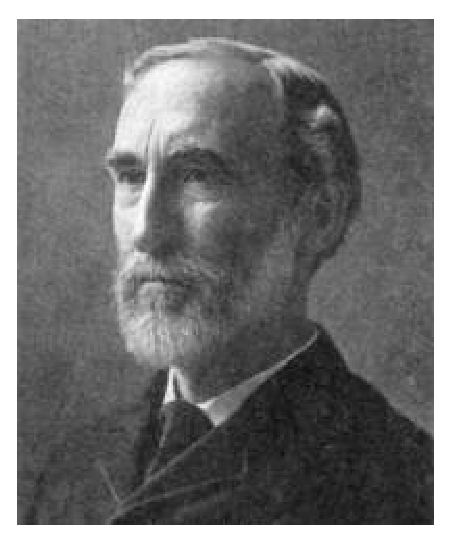
\includegraphics[width=3truecm]{figures/WGibbs.eps}
\small\begin{flushleft}\BrickRed{J.W.~Gibbs (1839-1903)}\end{flushleft}\normalsize
\end{columns}
}}}}

\pause
\vglue .9truecm
\centerline{{\bf $\pi(\theta,\lambda|x)$ is
a stationary distribution for this transition}}

\end{slide}\begin{slide}
\slidetitle{Implementation}

\begin{enumerate}
\item Derive efficient decomposition of the joint distribution into simulable conditionals
(mixing behavior, {\sf acf()}, blocking, \&tc.)

\pause\vs
\item Find when to stop the algorithm
(mode chasing, missing mass, shortcuts, \&tc.)

\end{enumerate}

\end{slide}\begin{frame}
\frametitle{Simple Example: iid
$\mathscr{N}(\mu,\sigma^2)$ Observations}
  When $y_1,\ldots,y_n \stackrel{\text{iid}}{\sim}
  \mathscr{N}(\mu,\sigma^2)$ with both $\mu$ and $\sigma$ unknown, the posterior in
  $(\mu, \sigma^2)$ is conjugate outside a standard family

\pause
\begin{block}{But...}
\begin{description}
\item $\mu|\by,\sigma^2$ $\sim \mathscr{N}\left(\mu\left|\frac{1}{n}
	\sum_{i=1}^n y_i, \frac{\sigma^2}{n}\right.\right.)$
\item $\sigma^2|\by,\mu$ $\sim \mathscr{IG}\left(\sigma^2 \left|\frac{n}{2}-1,
	\frac{1}{2}\sum_{i=1}^n (y_i-\mu)^2 \right.\right)$
\end{description}
assuming constant (improper) priors on both $\mu$ and $\sigma^2$
\end{block}
\begin{itemize}
\item Hence we may use the Gibbs sampler for simulating from the posterior
      of $(\mu,\sigma^2)$
\end{itemize}

\end{frame}

\begin{slide}\slidetitle{Gibbs output analysis}

\begin{example}[Cauchy posterior]
$$
\pi(\mu|\mathscr{D}) \propto \frac{e^{-\mu^2/20}}{(1+(x_1-\mu)^2)(1+(x_2-\mu)^2)}
$$
is marginal of
$$
\pi(\mu,\boldsymbol{\omega} |\mathscr{D}) \propto e^{-\mu^2/20} \times \prod_{i=1}^2 e^{-\omega_i[1+(x_i-\mu)^2]}\,.
$$
\pause
Corresponding conditionals
\small
\begin{eqnarray*}
(\omega_1,\omega_2) | \mu  & \sim & \mathscr{E}xp(1+(x_1-\mu)^2) \otimes \mathscr{E}xp(1+(x_2-\mu))^2) \\
\mu | \boldsymbol{\omega}  & \sim & \mathscr{N}\left(\sum_i\omega_i x_i/(\sum_i\omega_i +1/20),1/(2\sum_i\omega_i +1/10)\right)
\end{eqnarray*}
\normalsize
\end{example}

\end{slide}\begin{slide}
\slidetitle{Gibbs output analysis (cont'd)}

\centerline{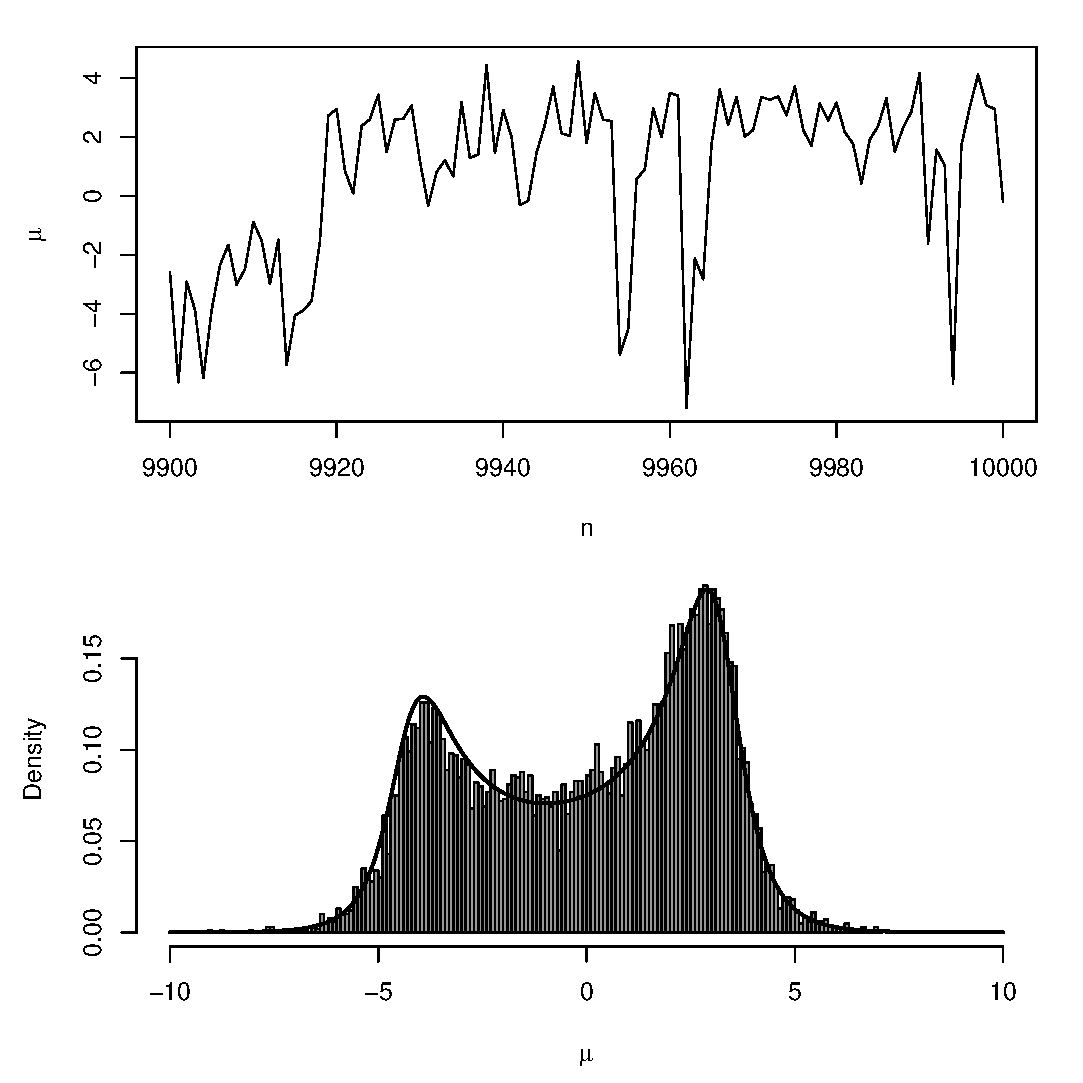
\includegraphics[width=7.5cm]{figures/simplegibbs.eps}}

\end{slide}\begin{slide}
\slidetitle{Generalisation}

Consider several groups of parameters, 
$\theta,\lambda_1,\allowbreak\ldots,\lambda_p$, such that
\[
\pi(\theta|x) = \int\ldots\int \pi(\theta,\lambda_1,\ldots,\lambda_p|x)
   \,d\lambda_1 \cdots \,d\lambda_p
\]
or simply divide $\theta$ in 
$$
(\theta_1,\ldots,\theta_p)
$$

\end{slide}\begin{slide}
\slidetitle{The general Gibbs sampler}

For a joint distribution $\pi(\theta)$ with full conditionals
$\pi_1,\ldots,\pi_p$,

\colorbox{LightGrey}{\makebox[0.9\textwidth][c]{\parbox{0.85\textwidth}{
{\sf
Given $(\theta_1^{(t)},\ldots,\theta_p^{(t)})$, simulate
\begin{itemize}
%\renewcommand{\theenumi}{\arabic{enumi}.}

\item[1.]  $\theta_1^{(t+1)} \sim
\pi_1(\theta_1|\theta_2^{(t)},\ldots,\theta_p^{(t)})$,

\item[2.] $\theta_2^{(t+1)} \sim
\pi_2(\theta_2|\theta_1^{(t+1)},\theta_3^{(t)},\ldots,\theta_p^{(t)})$,

\item[{\ }] $\qquad\qquad\vdots$

\item[p.] $\theta_p^{(t+1)} \sim
\pi_p(\theta_p|\theta_1^{(t+1)},\ldots,\theta_{p-1}^{(t+1)})$.
\end{itemize}
}}}}

\bigskip
\centerline{{{\bf Then $\theta^{(t)} \rightarrow \theta \sim \pi $}}}

\end{slide}
\normalsize \subsection{Variable selection}
\begin{slide}\slidetitle{Variable selection}

Back to regression: one dependent random variable $y$ and a set 
$\{x_1,\ldots,x_k\}$ of $k$ explanatory variables.

\pause
\vs\BrickRed{{\bf Question: }} Are all $x_i$'s involved in the regression?

\pause
\vs {\bf Assumption}: every subset $\{i_1,\ldots,i_q\}$ of 
$q$ $(0\le q\le k)$ explanatory variables, $\{\mathbf{1}_n,x_{i_1},
\ldots,x_{i_q}\}$, is a proper set of explanatory variables for the regression of $y$
[intercept included in every corresponding model] 

\pause
\begin{block}{Computational issue} 
\centerline{$2^k$ models in competition...}
\end{block}

\end{slide}\begin{slide}\slidetitle{Model notations}

\begin{enumerate}
\item $$
X=\left[\begin{matrix}\mathbf{1}_n &x_1 &\cdots &x_k \end{matrix}\right]
$$
is the matrix containing $\mathbf{1}_n$ and all the $k$ potential predictor variables

\item Each model $\mathfrak{M}_\gamma$ associated with binary indicator vector 
$\gamma\in\Gamma=\{0,1\}^k$ where $\gamma_i=1$ means that the variable $x_i$ is included in 
the model $\mathfrak{M}_\gamma$

\item $q_\gamma = \mathbf{1}_n^\tee \gamma$ number of variables included in the model $\mathfrak{M}_\gamma$

\item $t_1(\gamma)$ and $t_0(\gamma)$ indices of 
variables included in the model and indices of variables not included in the model
\end{enumerate}

\end{slide}\begin{slide}\slidetitle{Model indicators}

For $\beta\in\mathbb{R}^{k+1}$ and $X$, 
we define $\beta_\gamma$ as the subvector
$$
\beta_{\gamma}=\left(\beta_0,\left(\beta_i\right)_{i\in t_1(\gamma)}\right)
$$ 
and $X_{\gamma}$ as the submatrix of $X$ where only the column $\mathbf{1}_n$ 
and the columns in $t_1(\gamma)$ have been left.

\end{slide}\begin{slide}\slidetitle{Models in competition}

The model $\mathfrak{M}_\gamma$ is thus defined as 
$$
y|\gamma,\beta_\gamma,\sigma^2,X\sim\mathscr{N}_n\left(X_{\gamma}\beta_{\gamma},\sigma^2I_n\right)
$$
where $\beta_{\gamma}\in\mathbb{R}^{q_\gamma+1}$ and $\sigma^2\in\mathbb{R}^*_+$ 
are the unknown 
parameters.

\pause\vs
\begin{block}{Warning}
$\sigma^2$ is common to all models and thus uses the same prior for all models
\end{block}

\end{slide}\begin{slide}\slidetitle{Informative $G$-prior}

Many ($2^k$) models in competition: we cannot expect 
a practitioner to specify a prior on every $\mathfrak{M}_\gamma$ 
in a completely subjective and autonomous manner. 

\vs \BurntOrange{{\bf Shortcut:}} We derive {\em all} priors from a single 
global prior associated with the so-called {\em full model} that corresponds 
to $\gamma=(1,\dots,1)$. 

\end{slide}\begin{slide}\slidetitle{Prior definitions}

\begin{enumerate}
\renewcommand{\theenumi}{(\roman{enumi})}
\item For the full model, Zellner's $G$-prior:
$$
\beta|\sigma^2,X\sim\mathscr{N}_{k+1}(\tilde\beta,c\sigma^2(X^\tee X)^{-1})
\quad\text{and}\quad
\sigma^2\sim \pi(\sigma^2|X)=\sigma^{-2}
$$
\item For each model $\mathfrak{M}_\gamma$, the prior distribution of $\beta_{\gamma}$ 
conditional on $\sigma^2$ is fixed as
$$
\beta_\gamma|\gamma,\sigma^2 \sim \mathcal{N}_{q_\gamma+1}\left(\tilde\beta_{\gamma},
	c\sigma^2\left(X_{\gamma}^\tee X_{\gamma}\right)^{-1}\right)\,,
$$
where $\tilde \beta_\gamma=\left(X_\gamma^TX_\gamma\right)^{-1}X_\gamma^T\tilde\beta$
and same prior on $\sigma^2$. 
\end{enumerate}

\end{slide}\begin{slide}\slidetitle{Prior completion}

The joint prior for model $\mathfrak{M}_\gamma$ is
the improper prior
\begin{eqnarray*}
\pi(\beta_\gamma,\sigma^2|\gamma) 
&\propto& \left(\sigma^2\right)^{-(q_\gamma+1)/2-1}
   \exp\left[-\frac{1}{2(c\sigma^2)}\left(\beta_{\gamma}-\tilde\beta_{\gamma}\right)^\tee \right.\\
&&\quad \left.(X_{\gamma}^\tee X_{\gamma})\left(\beta_{\gamma}-\tilde\beta_{\gamma}\right)\right]\,.
\end{eqnarray*}

\end{slide}\begin{slide}\slidetitle{Prior competition (2)}

Infinitely many ways of defining a prior on the model index 
$\gamma$: choice of uniform prior $\pi(\gamma|X)=2^{-k}$.

\vs Posterior distribution of $\gamma$ central to 
variable selection since it is proportional to marginal density of $y$ on 
$\mathfrak{M}_\gamma$ (or {\em evidence} of $\mathfrak{M}_\gamma$)
\small
\begin{eqnarray*}
\pi(\gamma|y,X) & \propto & f(y|\gamma,X)\pi(\gamma|X) \propto f(y|\gamma,X) \\
                & = & \int\left(\int f(y|\gamma,\beta,\sigma^2,X)\pi(\beta|\gamma,
			\sigma^2,X)\,\text{d}\beta\right)\pi(\sigma^2|X)\,\text{d}\sigma^2\,.
\end{eqnarray*}
\normalsize

\end{slide}\begin{slide}
\small \begin{eqnarray*}
f(y|\gamma,\sigma^2,X) &=& \int f(y|\gamma,\beta,\sigma^2)\pi(\beta|\gamma,\sigma^2)\,\text{d}\beta \\
                       &=& (c+1)^{-(q_\gamma+1)/2}(2\pi)^{-n/2}\left(\sigma^2\right)^{-n/2} 
				\,\exp\left(-\frac{1}{2\sigma^2}y^\tee y \right.\\
                       & &\ \left.+\frac{1}{2\sigma^2(c+1)}\left\{c y^\tee X_{\gamma}\left(X_{\gamma}^\tee 
			     X_{\gamma}\right)^{-1}X_{\gamma}^\tee y
                       -\tilde\beta_{\gamma}^\tee X_{\gamma}^\tee X_{\gamma} \tilde\beta_{\gamma}\right\}\right)\,,
\end{eqnarray*}
\normalsize
this posterior density satisfies
\begin{eqnarray*}
\pi(\gamma|y,X) &\propto& (c+1)^{-(q_\gamma+1)/2}\left[y^\tee y-\frac{c}{c+1}y^\tee X_{\gamma}\left(X_{\gamma}^\tee 
			X_{\gamma}\right)^{-1}X_{\gamma}^\tee y\right. \\
                &&\quad \left.-\frac{1}{c+1}\tilde\beta_{\gamma}^\tee X_{\gamma}^\tee X_{\gamma} \tilde\beta_{\gamma}\right]^{-n/2}.
\end{eqnarray*}
\normalsize

\end{slide}\begin{frame} \frametitle{Pine processionary caterpillars} 

\begin{center}
\footnotesize
\begin{tabular}{l c| r}
  $t_1(\gamma)\ $ && $\ \pi(\gamma|\by,X)$ \\
 \hline 0,1,2,4,5 && 0.2316 \\
 0,1,2,4,5,9   && 0.0374 \\
 0,1,9         && 0.0344 \\
 0,1,2,4,5,10  && 0.0328 \\
 0,1,4,5       && 0.0306 \\
 0,1,2,9       && 0.0250 \\
 0,1,2,4,5,7   && 0.0241 \\
 0,1,2,4,5,8   && 0.0238 \\
 0,1,2,4,5,6   && 0.0237 \\
 0,1,2,3,4,5   && 0.0232 \\
 0,1,6,9       && 0.0146 \\
 0,1,2,3,9     && 0.0145 \\
 0,9           && 0.0143 \\
 0,1,2,6,9     && 0.0135 \\
 0,1,4,5,9     && 0.0128 \\
 0,1,3,9       && 0.0117 \\
 0,1,2,8       && 0.0115 \\
\end{tabular}                      
\normalsize
\end{center}

\end{frame}\begin{frame} \frametitle{Pine processionary caterpillars (cont'd)}

\begin{block}{Interpretation} Model $\mathfrak{M}_\gamma$ with the highest posterior probability
is $t_1(\gamma)=(1,2,4,5)$, which corresponds to the variables
\begin{itemize}
\item[-] altitude,
\item[-] slope,
\item[-] height of the tree sampled in the center of the area, and
\item[-] diameter of the tree sampled in the center of the area.
\end{itemize}
\end{block}

\pause\vs
Corresponds to the five variables identified in the {\sf R} regression output

\end{frame}\begin{slide}
\slidetitle{Noninformative extension}

For Zellner noninformative prior with $\pi(c)=1/c$, we have
\begin{eqnarray*}
\pi(\gamma|y,X)&\propto&\sum_{c=1}^\infty c^{-1}(c+1)^{-(q_\gamma+1)/2}\left[y^\tee y-\right.\nonumber\\
&&\quad \left.\frac{c}{c+1}y^\tee X_{\gamma}\left(X_{\gamma}^\tee X_{\gamma}\right)^{-1}X_{\gamma}^\tee y\right]^{-n/2}.
\end{eqnarray*}

\end{slide}\begin{frame} \frametitle{Pine processionary caterpillars}

\begin{center}
\footnotesize
\begin{tabular}{l c|r}
 $t_1(\gamma)$ && $\ \pi(\gamma|\by,X)$ \\ 
\hline 
 0,1,2,4,5      && 0.0929 \\
 0,1,2,4,5,9    && 0.0325 \\
 0,1,2,4,5,10   && 0.0295 \\
 0,1,2,4,5,7    && 0.0231 \\
 0,1,2,4,5,8    && 0.0228 \\
 0,1,2,4,5,6    && 0.0228 \\
 0,1,2,3,4,5    && 0.0224 \\
 0,1,2,3,4,5,9  && 0.0167 \\
 0,1,2,4,5,6,9  && 0.0167 \\
 0,1,2,4,5,8,9  && 0.0137 \\
 0,1,4,5        && 0.0110 \\
 0,1,2,4,5,9,10 && 0.0100 \\
 0,1,2,3,9      && 0.0097 \\
 0,1,2,9        && 0.0093 \\
 0,1,2,4,5,7,9  && 0.0092 \\
 0,1,2,6,9      && 0.0092 \\
\end{tabular}
\normalsize
\end{center}

\end{frame}\begin{slide}
\slidetitle{Stochastic search for the most likely model}

When $k$ gets large, impossible to compute the 
posterior probabilities of the $2^k$ models. 

\pause\vs
Need of a tailored algorithm 
that samples from $\pi(\gamma|y,X)$ and 
selects the most likely models. 

\vs Can be done by Gibbs sampling, given the availability 
of the full conditional posterior probabilities of the $\gamma_i$'s.

If $\gamma_{-i}=(\gamma_1,\ldots,\gamma_{i-1},\gamma_{i+1},\ldots,\gamma_k)$ 
($1\le i\le k$) 
$$
\pi(\gamma_i|y,\gamma_{-i},X)\propto
\pi(\gamma|y,X)
$$
(to be evaluated in both $\gamma_i=0$ and $\gamma_i=1$)

\end{slide}\begin{slide}\slidetitle{Gibbs sampling for variable selection}

\colorbox{LightGrey}{\makebox[0.9\textwidth][c]{\parbox{0.85\textwidth}{
\begin{sffamily}
\begin{itemize}
\item[ ] {\bfseries Initialization:} Draw $\gamma^0$ from the uniform distribution on $\Gamma$
\pause\vspace{0.5cm} \item[ ] {\bfseries Iteration $t$:} Given $(\gamma_1^{(t-1)},\ldots,\gamma_k^{(t-1)})$, generate
\begin{itemize}
\vspace{0.25cm} \item[1.] {{ \ $\gamma_1^{(t)}$ according to 
$\pi(\gamma_1|y,\gamma_2^{(t-1)},\ldots,\gamma_k^{(t-1)},X)$ }}
\vspace{0.25cm} \item[2.] {{ \ $\gamma_2^{(t)}$ according to 
$\pi(\gamma_2|y,\gamma_1^{(t)},\gamma_3^{(t-1)},\ldots,\gamma_k^{(t-1)},X)$ }}
\vspace{0.25cm} \item[{\ }] $\qquad\qquad\vdots$
\vspace{0.25cm} \item[p.] {{ \ $\gamma_k^{(t)}$ according to 
$\pi(\gamma_k|y,\gamma_1^{(t)},\ldots,\gamma_{k-1}^{(t)},X)$ }}
\end{itemize}
\end{itemize}
\end{sffamily}
}}}

\end{slide}\begin{slide}\slidetitle{MCMC interpretation}

After $T\gg 1$ MCMC iterations,
output used to approximate the posterior probabilities $\pi(\gamma|y,X)$ 
by empirical averages 
$$
\widehat{\pi}(\gamma|y,X)=\left(\frac{1}{T-T_0+1}\right)\sum_{t=T_0}^T \mathbb{I}_{\gamma^{(t)}=\gamma}.
$$
where the $T_0$ first values are eliminated as {\em burnin}.

\pause\vs
And approximation of the probability to include $i$-th variable,
$$
{\widehat{P}}^\pi(\gamma_i=1|y,X)=\left(\frac{1}{T-T_0+1}\right)\sum_{t=T_0}^T 
\mathbb{I}_{\gamma^{(t)}_i=1}\,.
$$
\end{slide}\begin{slide}\slidetitle{Pine processionary caterpillars}

\begin{center}
\small
\begin{tabular}{l c|r|r}
 $\gamma_i$    && $\ {\widehat{P}}^\pi(\gamma_i=1|\by,X)$ 
& $\ {\widehat{P}}^\pi (\gamma_i=1|\by,X)$\\                                                    
\hline $\gamma_1$    && 0.8624 & 0.8844 \\
 $\gamma_2$    && 0.7060 & 0.7716 \\
 $\gamma_3$    && 0.1482 & 0.2978 \\
 $\gamma_4$    && 0.6671 & 0.7261 \\
 $\gamma_5$    && 0.6515 & 0.7006 \\
 $\gamma_6$    && 0.1678 & 0.3115 \\
 $\gamma_7$    && 0.1371 & 0.2880 \\
 $\gamma_8$    && 0.1555 & 0.2876 \\
 $\gamma_9$    && 0.4039 & 0.5168 \\
 $\gamma_{10}$ && 0.1151 & 0.2609 \\
\end{tabular}
\normalsize

Probabilities of inclusion with both informative
$(\tilde\beta=0_{11},c=100)$ and noninformative  Zellner's priors 
\end{center}


\end{slide}

\section{Generalized linear models}
\begin{slide}\slidetitle{Generalized linear models}
\tableofcontents[sectionstyle=show/hide,subsectionstyle=show/shaded/hide]

\end{slide}
\subsection{Generalisation of linear models}
\begin{slide}\slidetitle{Generalisation of Linear Models}

Linear models model connection between a response variable $y$ and a set $x$ of explanatory
variables by a linear dependence relation with [approximately] normal perturbations. 

\pause
\vs Many instances where either of these assumptions not appropriate, e.g.~ when the support of $y$
restricted to $\mathbb{R}_+$ or to $\mathbb{N}$.

\end{slide}\begin{slide}
\slidetitle{{\sf bank}}

Four measurements on 100 genuine Swiss banknotes and 100 counterfeit ones:
\begin{itemize}
\item[] $x_1$ length of the bill (in mm),
\item[] $x_2$ width of the left edge (in mm),
\item[] $x_3$ width of the right edge (in mm),
\item[] $x_4$ bottom margin width (in mm).
\end{itemize}

Response variable $y$: status of the banknote [$0$ for genuine and $1$ 
for counterfeit] 

\pause\vs
Probabilistic model that predicts counterfeiting based on the four measurements

\end{slide}\begin{slide}
\slidetitle{The impossible linear model}

Example of the influence of $x_4$ on $y$

Since  $y$ is binary, 
$$
y|x_4 \sim \mathscr{B}(p(x_4))\,,
$$
\MidnightBlue{{\bf \copyright~Normal model is impossible}}

\smallskip\pause
Linear dependence in $p(x)=\mathbb{E}[y|x]$'s
$$
p(x_{4i})=\beta_0+\beta_1 x_{4i}\,,
$$
\pause estimated [by MLE] as
$$
\hat p_i=-2.02+0.268\,x_{i4}
$$
which gives $\hat p_i=.12$ for $x_{i4}=8$ and ... \pause
$\hat p_i=1.19$ for $x_{i4}=12$!!!

\MidnightBlue{{\bf \copyright~Linear dependence is impossible}}

\end{slide}\begin{slide}
\slidetitle{Generalisation of the linear dependence}

Broader class of models to cover various dependence structures. 

\pause
\vs Class of {\em generalised linear models} (GLM) where
$$
y|\bx,\beta \sim f(y|\bx^\tee\beta)\,.
$$
i.e., dependence of $y$ on $\bx$ partly {\em linear} 

\end{slide}\begin{slide}
\slidetitle{Notations}

Same as in linear regression chapter, with $n$--sample
$$
\by=\left(y_1,\ldots,y_n\right)
$$ 
and corresponding explanatory variables/covariates
$$
X=\left[\begin{array}{cccc}
 x_{11} & x_{12} & \ldots & x_{1k} \\
 x_{21} & x_{22} & \ldots & x_{2k} \\
 x_{31} & x_{32} & \ldots & x_{3k} \\
 \vdots & \vdots & \vdots & \vdots \\
 x_{n1} & x_{n2} & \ldots & x_{nk}
\end{array}\right]
$$

\end{slide}\begin{slide}
\slidetitle{Specifications of GLM's}

\begin{definition}[GLM]
A GLM is a conditional model specified by two functions:
\begin{enumerate}
\item the density $f$ of $y$ given $\bx$ parameterised by its expectation parameter $\mu=\mu(\bx)$ 
[and possibly its dispersion parameter $\varphi=\varphi(\bx)$]
\pause
\item the {\em link} $g$ between the mean $\mu$ and the explanatory variables, written customarily as $g(\mu)=\bx^\tee\beta$
or, equivalently, $\mathbb{E}[y|\bx,\beta] =g^{-1}(\bx^\tee\beta)$. 
\end{enumerate}
\end{definition}

\pause
\vs For identifiability reasons, $g$ needs to be bijective. 

\end{slide}\begin{slide}
\slidetitle{Likelihood}

Obvious representation of the likelihood 
$$
\ell(\beta,\varphi|\by,X) = \prod_{i=1}^nf\left(y_i|\bx^{i\tee}\beta,\varphi\right)
$$
with parameters $\beta\in\mathbb{R}^k$ and $\varphi>0$.

\end{slide}\begin{slide}
\slidetitle{Examples}

\begin{itemize}
\item \MidnightBlue{Ordinary linear regression}

Case of GLM where 
$$
g(x)=x,\ 
\varphi=\sigma^2,\quad\text{and}\quad
\by|X,\beta,\sigma^2\sim\mathscr{N}_n(X\beta,\sigma^2).
$$
\end{itemize}

\end{slide}\begin{slide}
\slidetitle{Examples (2)}

Case of binary and binomial data, when 
$$
y_i|\bx^i\sim\mathscr{B}(n_i,p(\bx^i))
$$
with known $n_i$

\begin{itemize}
\item \MidnightBlue{Logit [or logistic regression] model}

Link is {\em logit transform} on probability of success
$$
g(p_i)=\log(p_i/(1-p_i))\,,
$$
with likelihood 
\footnotesize \begin{eqnarray*}
&& \prod_{i=1}^n\left(\begin{array}{l} n_i \\ y_i \end{array}\right)
\left(\frac{\exp(\bx^{i\tee}\beta)}{1+\exp(\bx^{i\tee}\beta)}\right)^{y_i}
\left(\frac{1}{1+\exp(\bx^{i\tee}\beta)}\right)^{n_i-y_i}\\
&&\qquad \propto \exp \left\{ \sum_{i=1}^n y_i\bx^{i\tee}\beta \right\}
\bigg/ \prod_{i=1}^n \left(1+\exp(\bx^{i\tee}\beta)\right)^{n_i-y_i}\nonumber
\end{eqnarray*}
\normalsize
\end{itemize}

\end{slide}\begin{slide}
\slidetitle{Canonical link}

Special link function $g$ that appears in the natural exponential family representation of the density
$$
g^\star(\mu)=\theta
\quad \text{if}\quad f(y|\mu)
\propto \exp \{T(y)\cdot\theta-\Psi(\theta)\}
$$

\pause
\begin{example}Logit link is canonical for the binomial model, since
$$
f(y_i|p_i) = {n_i \choose y_i}\,\exp\left\{ y_i\,\log\left( \frac{p_i}{1-p_i}\right)+n_i\,\log(1-p_i)\right\}\,, 
$$
and thus
$$
\theta_i = \log p_i/(1-p_i)
$$\end{example}

\end{slide}\begin{slide}[label=Probex]
\slidetitle{Examples (3)}

Customary to use the canonical link, but only customary ...

\begin{itemize}
\item \MidnightBlue{Probit model}

Probit link function given by
$$
g(\mu_i)=\Phi^{-1}(\mu_i)
$$
where $\Phi$ standard normal cdf

Likelihood
$$
\ell(\beta|\by,X)\propto \prod_{i=1}^n \Phi(\bx^{i\tee}\beta)^{y_i} (1-\Phi(\bx^{i\tee}\beta))^{n_i-y_i}\,.
$$

\end{itemize}\hyperlink{Proful}{\beamergotobutton{Full processing}}

\end{slide}\begin{slide}[label=LLintro]
\slidetitle{Log-linear models}

Standard approach to describe associations between several {\em categorical} 
variables, i.e, variables with finite support
 
Sufficient statistic: {\em contingency table}, made of the
cross-classified counts for the different categorical 
variables.\hyperlink{LLmdL}{\beamergotobutton{Full entry to loglinear models}}

\pause\footnotesize
\begin{example}[Titanic survivors]
{\footnotesize{\tt{\MidnightBlue{
\begin{center}\begin{tabular}{c|c|cc|cc}
\hline
        &&Child&&Adult&\\
Survivor&Class  &Male &Female &Male &Female\\
\hline
  &1st     &0      &0 &118 &4\\
  &2nd     &0      &0 &154 &13\\
No &3rd    &35     &17 &387 &89\\
  &Crew    &0      &0 &670 &3\\
\hline
  &1st     &5      &1  &57 &140\\
  &2nd    &11     &13  &14 &80\\
Yes &3rd    &13     &14  &75 &76\\
  &Crew    &0      &0  &192 &20\\
\hline
\end{tabular}\end{center}
}}}}
\end{example}\normalsize


\end{slide}\begin{slide}\slidetitle{Poisson regression model}

\begin{enumerate}
\item Each count $y_i$ is Poisson with mean $\mu_i=\mu(\bx_i)$ 
\item Link function
connecting $\mathbb{R}^+$ with $\mathbb{R}$, e.g.~logarithm
$g(\mu_i)=\log(\mu_i)$. 
\end{enumerate}

\pause\vs Corresponding likelihood 
\small
$$
\ell(\beta|y,X)=\prod_{i=1}^n\left(\frac{1}{y_i!}\right)\exp\left\{
y_i \bx^{i\tee}\beta-\exp(\bx^{i\tee}\beta)\right\}\,.
$$
\normalsize

\end{slide}\subsection{Metropolis--Hastings algorithms}\begin{slide}[label=MCMC.0]
\slidetitle{Metropolis--Hastings algorithms}

\hfill\hyperlink{Convass}{\beamergotobutton{Convergence assessment}}

\vs Posterior inference in GLMs harder than for linear models

\pause
\vs \copyright~Working with a GLM requires specific numerical or simulation tools 
[E.g., {\sf GLIM} in classical analyses] 

\pause
\vs Opportunity to introduce universal MCMC method: \MidnightBlue{{\em Metropolis--Hastings} algorithm}

\end{slide}\begin{slide}
\slidetitle{Generic MCMC sampler}

\begin{itemize}
\item Metropolis--Hastings algorithms are generic/down-the-shelf MCMC algorithms 
\item Only require likelihood up to a constant \Sepia{[difference with Gibbs sampler] }

\item can be tuned with a wide range of possibilities \Sepia{[difference with Gibbs sampler \&\ blocking]}

\item natural extensions of standard simulation algorithms: %like accept-reject or sampling-importance-resampling: 
based on the choice of a {\em proposal} 
distribution \Sepia{[difference in Markov proposal $q(x,y)$ and acceptance]}
\end{itemize}

\end{slide}\begin{slide}
\slidetitle{Why Metropolis?}

Originally introduced by Metropolis, Rosenbluth, Rosenbluth, Teller and Teller
in a setup of optimization on a discrete state-space.  All authors involved in Los Alamos during and after WWII:
\pause\small
\begin{itemize}
\item Physicist and mathematician, Nicholas Metropolis is considered (with Stanislaw Ulam) to be the father
of Monte Carlo methods. 
\item Also a physicist, Marshall Rosenbluth worked on the development of the hydrogen (H) bomb 
\item Edward Teller was one of the first scientists to work on the Manhattan Project
that led to the production of the A bomb. Also managed to design with Ulam the H bomb.
\end{itemize}\normalsize

\end{slide}\begin{slide}
\slidetitle{Generic Metropolis--Hastings sampler}

For {\em target} $\pi$ and proposal kernel $q(x,y)$

\begin{block}{\sffamily
\begin{itemize}
\small
\item[ ] {\bfseries Initialization:} Choose an arbitrary $x^{(0)}$
\pause
\item[ ] {\bfseries Iteration $t$:} 
\normalsize
\begin{enumerate}
\item Given $x^{(t-1)}$, generate $\tilde x \sim q(x^{(t-1)},x)$
\item Calculate 
$$
\rho(x^{(t-1)},\tilde x)=\min\left(\frac{\pi(\tilde x)/q(x^{(t-1)},\tilde x)}{\pi(x^{(t-1)})/q(\tilde x,x^{(t-1)})},1\right)
$$
\item  With probability $\rho(x^{(t-1)},\tilde x)$ accept $\tilde x$ and set $x^{(t)}=\tilde x$;\\
otherwise reject $ \tilde x$ and set $x^{(t)}=x^{(t-1)}$.
\end{enumerate}
\end{itemize}
}\end{block}

\end{slide}\begin{slide}
\slidetitle{Universality}

Algorithm only needs to simulate from 
$$q$$ which can be chosen [almost!] arbitrarily, i.e.~unrelated with $\pi$ 
[$q$ also called {\em instrumental} distribution]

\vs
{\bf Note:} $\pi$ and $q$ known up to proportionality terms ok since proportionality constants cancel in $\rho$. 

\end{slide}\begin{slide}
\slidetitle{Validation}

\begin{block}{Markov chain theory}
Target $\pi$ is stationary distribution of Markov chain $(x^{(t)})_t$ because
probability $\rho(x,y)$ satisfies \BurntOrange{{\em detailed balance equation}}
$$
\pi(x) q(x,y) \rho(x,y) = \pi(y) q(y,x) \rho(y,x)
$$
{\em [Integrate out $x$ to see that $\pi$ is stationary]}
\end{block}

\vs\pause
For convergence/ergodicity, Markov chain must be {\em irreducible}: $q$ has positive probability of reaching all areas 
with positive $\pi$ probability in a finite number of steps.

\end{slide}\begin{slide}
\slidetitle{Choice of proposal}

Theoretical guarantees of convergence very high, but choice of $q$ is crucial in practice. \pause
Poor choice of $q$ may result in 
\begin{itemize}
\item very high rejection rates, with very few moves of the Markov 
chain $(x^{(t)})_t$ hardly moves, or in 
\pause
\item a myopic exploration of the support of $\pi$, that is, in a dependence on
the starting value $x^{(0)}$, with the chain stuck in a neighbourhood mode to $x^{(0)}$.
\end{itemize}

\pause
\begin{block}{Note: hybrid MCMC}
Simultaneous use of different kernels valid {\em and} recommended
\end{block}

\end{slide}\begin{slide}
\slidetitle{The independence sampler}

Pick proposal $q$ that is independent of its first argument,
$$
q(x,y)=q(y)
$$
$\rho$ simplifies into
$$
\rho(x,y)=\min\left(1,\frac{\pi(y)/q(y)}{\pi(x)/q(x)}\right)\,.
$$

\begin{block}{Special case: $q\propto\pi$}
Reduces to $\rho(x,y)=1$ and iid sampling
\end{block}

\pause Analogy with Accept-Reject algorithm where $\max \pi/q$
replaced with the current value $\pi(x^{(t-1)})/q(x^{(t-1)})$ 
but sequence of accepted $x^{(t)}$'s not i.i.d.

\end{slide}\begin{slide}
\slidetitle{Choice of $q$}

Convergence properties highly dependent on $q$. 
\begin{itemize}
\item $q$ needs to be positive everywhere on the support of $\pi$
\item for a good exploration of this support, $\pi/q$ needs to be bounded. 
\end{itemize}

\vs\pause Otherwise, the chain takes too long to reach regions with low $q/\pi$ values. 

\end{slide}\begin{slide}
\slidetitle{The random walk sampler}

Independence sampler requires too much global information about $\pi$:
opt for a local gathering of information

\vs\pause Means exploration of the neighbourhood of the current value $x^{(t)}$
in search of other points of interest. 

\vs\pause Simplest exploration device is based on random walk dynamics.\\

\end{slide}\begin{slide}
\slidetitle{Random walks}

Proposal is a symmetric transition density 
$$
q(x,y)=q_{RW}(y-x)=q_{RW}(x-y)
$$

\vs\pause Acceptance probability $\rho(x,y)$ reduces to the simpler form
$$
\rho(x,y)=\min\left(1,\frac{\pi(y)}{\pi(x)}\right)\,.
$$
Only depends on the target $\pi$ 
{\em [accepts all proposed values that increase $\pi$]}

\end{slide}\begin{slide}
\slidetitle{Choice of $q_{RW}$}

Considerable flexibility in the choice of $q_{RW}$,
\begin{itemize}
\item tails: Normal versus Student's $t$
\item scale: size of the neighbourhood 
\end{itemize}

\vs\pause 
Can also be used for restricted support targets [with a waste of simulations near the boundary]

\vs\pause
Can be tuned towards an acceptance probability of $0.234$ at the {\em burnin} stage 
\Sepia{{\em [Magic number!]}}

\end{slide}\begin{slide}[label=Convass]
\slidetitle{Convergence assessment}

\BurntOrange{{\bf Capital question: How many iterations do we need to run???}}
\hfill\hyperlink{MCMC.0}{\beamerreturnbutton{MCMC debuts}}

\pause
\begin{itemize}
\item \MidnightBlue{{\bf Rule \# 1}} There is no absolute number of simulations, i.e.
$1,000$ is neither large, nor small.
\item \MidnightBlue{{\bf Rule \# 2}} It takes [much] longer to check for convergence 
than for the chain itself to converge.
\item \MidnightBlue{{\bf Rule \# 3}} MCMC is a {\em ``what-you-get-is-what-you-see"} algorithm: it 
fails to tell about unexplored parts of the space.
\item \MidnightBlue{{\bf Rule \# 4}} When in doubt, run MCMC chains in parallel and check for 
consistency.
\end{itemize}
\vs\pause
Many ``quick-\&-dirty" solutions in the literature, but not necessarily trustworthy.

\end{slide}\begin{slide}
\slidetitle{Prohibited dynamic updating}

\begin{itemize}
\item[$\lightning$] \MidnightBlue{
Tuning the proposal in terms of its past performances can only
be implemented at {\em burnin}, because otherwise this cancels Markovian convergence 
properties.}
\end{itemize}

\vs\pause
Use of several MCMC proposals together within a single
algorithm using circular or random design is ok.
It almost always brings an improvement compared with its individual components (at the cost
of increased simulation time)

\end{slide}
\begin{slide}\slidetitle{Effective sample size}

\Sepia{{\bf How many iid simulations from
$\pi$ are equivalent to $N$ simulations from the MCMC algorithm?}}

\vs\pause
Based on estimated $k$-th order auto-correlation,
$$
\rho_k = \mathrm{corr}\left(x^{(t)},x^{(t+k)} \right)\,,
$$
effective sample size
\small$$
N^\text{ess} = n\,\left(1+2\,\sum_{k=1}^{T_0} \hat\rho_k^2\right)^{-1/2}\,,
$$\normalsize
\begin{enumerate}
\item[{\Large $\lightning$}] Only partial indicator that fails to signal
chains stuck in one mode of the target 
\end{enumerate}

\end{slide}\subsection{The Probit Model}\begin{slide}[label=Proful]
\slidetitle{The Probit Model}

Likelihood\hyperlink{Probex}{\beamerreturnbutton{Recall Probit}}
$$
\ell(\beta|\by,X)\propto \prod_{i=1}^n \Phi(\bx^{i\tee}\beta)^{y_i} (1-\Phi(\bx^{i\tee}\beta))^{n_i-y_i}\,.
$$

\pause If no prior information available, resort to the flat prior 
$\pi(\beta)\propto 1$ and then obtain the posterior distribution
$$
\pi(\beta|\by,X) \propto \prod_{i=1}^n \Phi\left(\bx^{i\tee}\beta\right)^{y_i}\left(1-\Phi(\bx^{i\tee}\beta)\right)^{n_i-y_i}\,,
$$
nonstandard and simulated using MCMC techniques.

\end{slide}\begin{slide} 
\slidetitle{MCMC resolution}

\vs Metropolis--Hastings random walk sampler works well for binary regression problems with
small number of predictors

\vs Uses the maximum likelihood estimate
$\hat\beta$ as starting value and asymptotic (Fisher)
covariance matrix of the MLE, $\hat\Sigma$, as scale

\end{slide}
\begin{frame}[fragile]
\frametitle{MLE proposal}

{\sf R} function {\sf glm} very useful to get the maximum likelihood estimate of $\beta$ 
and its asymptotic covariance matrix $\hat\Sigma$.

\vs Terminology used in {\sf R} program\small
\begin{verbatim}
mod=summary(glm(y~X-1,family=binomial(link="probit")))
\end{verbatim}\normalsize 
with {\sf mod{\$}coeff[,1]} denoting $\hat\beta$ and {\sf mod{\$}cov.unscaled} $\hat\Sigma$.

\end{frame}
\begin{slide}
\slidetitle{MCMC algorithm}

\begin{block}{Probit random-walk Metropolis-Hastings}
\begin{itemize}{\sffamily
\item[] {\bfseries Initialization:} Set $\beta^{(0)}=\hat\beta$ and compute $\hat\Sigma$
\item[] {\bfseries Iteration $t$:} 
\begin{enumerate}
\item Generate $\tilde\beta \sim \mathscr{N}_{k+1}(\beta^{(t-1)},\tau\hat\Sigma)$
\item Compute
$$
\rho(\beta^{(t-1)},\tilde\beta)=\min\left(1,\frac{\pi(\tilde\beta|y)}{\pi(\beta^{(t-1)}|y)}\right)
$$
\item With probability $\rho(\beta^{(t-1)},\tilde\beta)$ set $\beta^{(t)}=\tilde\beta$;\\
otherwise set $\beta^{(t)}=\beta^{(t-1)}$.
\end{enumerate}
}\end{itemize}
\end{block}

\end{slide}
\begin{slide}
\slidetitle{{\sf bank}}

\begin{columns}\column{.35\textwidth}
Probit modelling  with no intercept over the
four measurements. 

Three different scales $\tau=1,0.1,10$: best mixing behavior is
associated with $\tau=1$.

Average of the parameters over $9,000$ iterations gives plug-in
estimate 
\column{.6\textwidth}
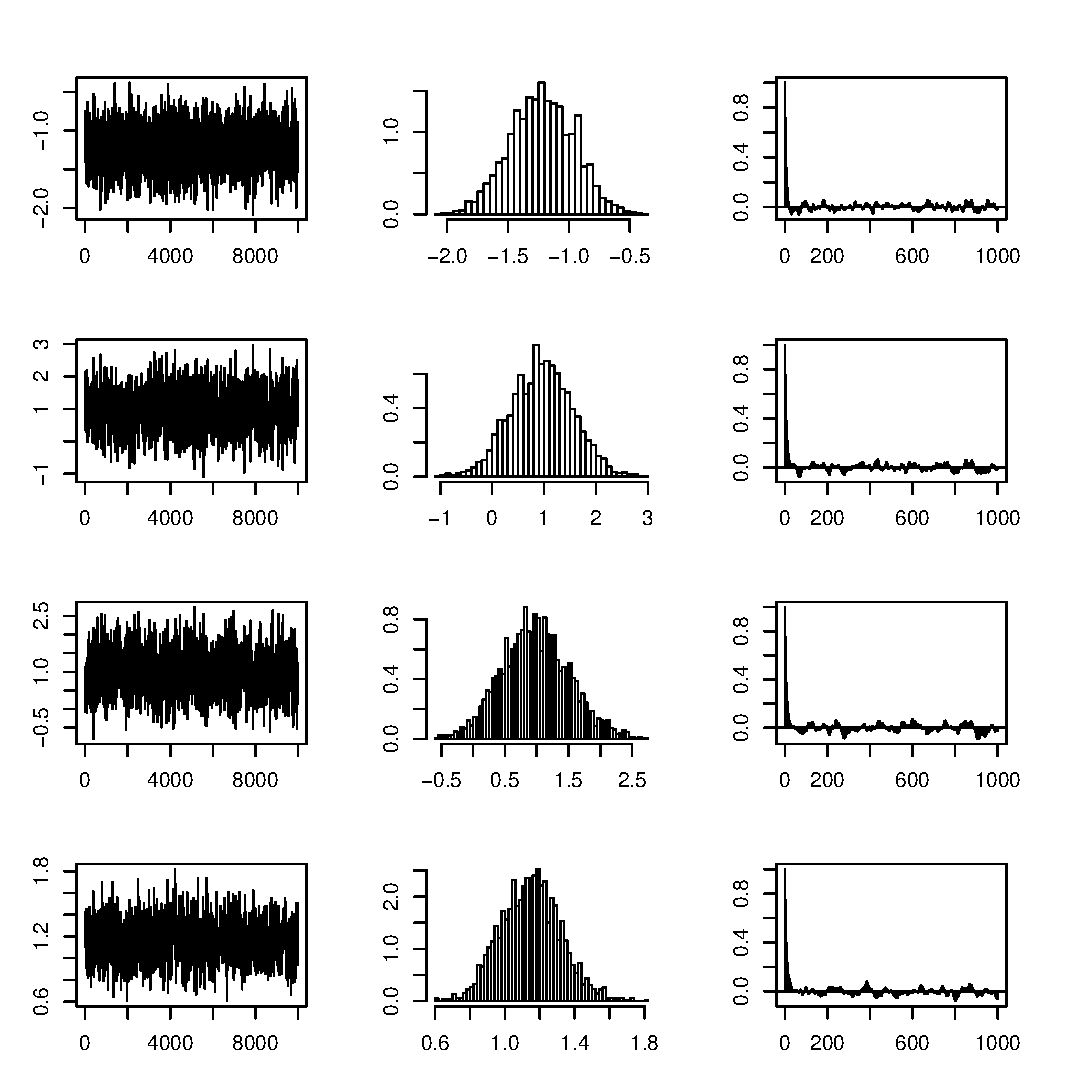
\includegraphics[width=6cm,height=6cm]{figures/hmflatprobit.eps}
\end{columns}
$$
\hat p_i=\Phi\left(-1.2193x_{i1}+0.9540x_{i2}+0.9795x_{i3}+ 1.1481x_{i4}\right).
$$

\end{slide}\begin{slide}
\slidetitle{G-priors for probit models}

Flat prior on $\beta$ inappropriate for comparison purposes
and Bayes factors. 

\pause Replace the flat prior with a hierarchical prior,
$$
\beta|\sigma^2,X\sim\mathscr{N}_k\left(0_k,\sigma^2(X^\tee X)^{-1}\right)
\quad\text{and}\quad
\pi(\sigma^2|X)\propto \sigma^{\RawSienna{-3/2}} \,,
$$
(almost) as in normal linear regression 

\vs\pause\begin{block}{Warning} 
The matrix $X^\tee X$ is {\em not} the Fisher information matrix
\end{block}

\end{slide}
\begin{slide}
\slidetitle{G-priors for testing}

Same argument as before: while $\pi$ is improper, use of the {\em same}
variance factor $\sigma^2$ in both models
means the normalising constant cancels in the Bayes factor.

\pause
\vs Posterior distribution of $\beta$\footnotesize
\begin{eqnarray*}
\pi(\beta|\by,X) & \propto & |X^\tee X|^{1/2} \Gamma((2k-1)/4)\left(\beta^\tee(X^\tee X)\beta\right)^{-(2k-1)/4}
	\pi^{-k/2} \nonumber \\
               && \times\prod_{i=1}^n\,\Phi( \bx^{i\tee}\beta)^{y_i}\left[1-\Phi(\bx^{i\tee}\beta)\right]^{1-y_i}
\end{eqnarray*}\normalsize
{\em [where $k$ matters!]}

\end{slide}\begin{slide}
\slidetitle{Marginal approximation}

Marginal\footnotesize
\begin{eqnarray*}
f(\by|X) & \propto & |X^\tee X|^{1/2}\,\pi^{-k/2}\Gamma\{(2k-1)/4\} \int \left(\beta^\tee(X^\tee X)\beta\right)^{-(2k-1)/4} \\
&& \quad\times\prod_{i=1}^n\,\Phi(\bx^{i\tee}\beta)^{y_i}\left[1-(\Phi(
\bx^{i\tee}\beta)\right]^{1-y_i}\,\text{d}\,\beta\,,
\end{eqnarray*}
\normalsize approximated by\footnotesize
\begin{align*}
\frac{|X^\tee X|^{1/2}}{\pi^{k/2}M}\,\sum_{m=1}^M &\left|\left|X\beta^{(m)}\right|\right|^{-(2k-1)/2}
\prod_{i=1}^n\,\Phi( \bx^{i\tee}{\beta^{(m)}})^{y_i} \left[1-\Phi(
\bx^{i\tee}{\beta^{(m)}})\right]^{1-y_i}\nonumber\\ &\times
\Gamma\{(2k-1)/4\}\,|\widehat V|^{1/2}(4\pi)^{k/2}\,
e^{\Red{+}({\beta^{(m)}}-\widehat\beta)^\tee \widehat
V^{-1}({\beta^{(m)}}-\widehat\beta)/4}\,,
\end{align*}\normalsize
where 
$$
\beta^{(m)} \sim \mathscr{N}_k(\widehat\beta,2\,\widehat V)
$$
with $\widehat\beta$ MCMC approximation of $\mathbb{E}^\pi[\beta|\by,X]$
and $\widehat    V$ MCMC approximation of $\mathbb{V}(\beta|\by,X)$.

\end{slide}\begin{slide}
\slidetitle{Linear hypothesis}

Linear restriction on $\beta$ 
$$
H_0:R\beta=r
$$
($r\in \mathbb{R}^q$, $R$ $q\times k$ matrix)
where $\beta^0$ is $(k-q)$ dimensional and $X_0$ and $\bx_0$ are linear transforms of $X$ and of $\bx$ of dimensions
$(n,k-q)$ and $(k-q)$. 

\vs Likelihood
$$
\ell(\beta^0|\by,X_0)\propto
\prod_{i=1}^n\,\Phi(\bx_0^{i\tee}\beta^0)^{y_i}
\left[1-\Phi(\bx_0^{i\tee}\beta^0)\right]^{1-y_i}\,,
$$

\end{slide}\begin{slide}
\slidetitle{Linear test}

Associated [projected] $G$-prior
$$
\beta^0|\sigma^2,X_0\sim\mathscr{N}_{k-q}\left(0_{k-q},\sigma^2(X_0^\tee
X_0)^{-1}\right)\, \quad \text{and} \quad \pi(\sigma^2|X_0)\propto
\sigma^{-3/2} \,,
$$

\vs\pause
Marginal distribution of $\by$ of the same type\footnotesize
\begin{eqnarray*}
f(\by|X_0) & \propto & |X_0^\tee X_0|^{1/2} \pi^{-(k-q)/2}\Gamma\left\{\frac{(2(k-q)-1)}{4}\right\} 
	\int \left|\left| X\beta^0\right|\right|^{-(2(k-q)-1)/2} \\
             && \quad\prod_{i=1}^n\,\Phi(\bx_0^{i\tee}\beta^0)^{y_i} \left[1-(\Phi(\bx_0^{i\tee}\beta^0)\right]^{1-y_i}
\text{d}\beta^0\,.
\end{eqnarray*}\normalsize

\end{slide}
\begin{frame}[fragile]
\frametitle{{\sf banknote}}

For $H_0:\beta_1=\beta_2=0$, $B^\pi_{10}=157.73$ [against $H_0$]

\vs Generic regression-like output:
\small
\begin{verbatim}
           Estimate  Post. var.  log10(BF)

X1          -1.1552   0.0631       4.5844 (****)
X2           0.9200   0.3299      -0.2875
X3           0.9121   0.2595      -0.0972
X4           1.0820   0.0287      15.6765 (****)

evidence against H0: (****) decisive, (***) strong,
(**) subtantial, (*) poor
\end{verbatim}
\normalsize

\end{frame}
\begin{slide}\slidetitle{Informative settings}

If prior information available on $p(\bx)$, transform 
into prior distribution on $\beta$ by technique of {\em 
imaginary observations:}

\vs\pause
Start with $k$ different values of the covariate vector, $\tilde \bx^1,\ldots,\tilde \bx^k$

For each of these values, the practitioner specifies 
\begin{itemize}
\item[(i)]  a prior guess $g_i$ at the probability $p_i$ associated with $\bx^i$;
\item[(ii)] an assessment of (un)certainty about that guess given by a number $K_i$ of
equivalent ``prior observations''.
\end{itemize}

\pause
\centerline{{\BurntOrange{\bf On how many imaginary observations did you build this guess?}}}

\end{slide}
\begin{slide}
\slidetitle{Informative prior}

$$
\pi(p_1,\ldots,p_k)\propto \prod_{i=1}^kp_i^{K_ig_i-1}(1-p_i)^{K_i(1-g_i)-1}
$$
translates into {\em [Jacobian rule]}
$$
\pi(\beta)\propto \prod_{i=1}^k\,\Phi(\tilde \bx^{i\tee}
\beta)^{K_ig_i-1}\left[ 1-\Phi(\tilde \bx^{i\tee}
\beta)\right]^{K_i(1-g_i)-1}\phi(\tilde \bx^{i\tee}\beta)
$$

\vs\pause

[Almost] equivalent to using the $G$-prior\footnotesize
$$
\beta\sim\mathscr{N}_k\left(0_k,\left[\sum_{j=1}^k \tilde
\bx^j\tilde \bx^{j\tee}\right]^{-1}\right)
$$\normalsize

\end{slide}
\subsection{The logit model}\begin{slide}
\slidetitle{The logit model}

Recall that [for $n_i=1$]
$$
y_i|\mu_i\sim\mathscr{B}(1,\mu_i),\quad \varphi=1
\quad\text{and}\quad
g(\mu_i)=\left(\frac{\exp(\mu_i)}{1+\exp(\mu_i)}\right).
$$

Thus
$$
\mathbb{P}(y_i=1|\beta)=\frac{\exp(\bx^{i\tee}\beta)}{1+\exp(\bx^{i\tee}\beta)}
$$
with likelihood 
\small$$
\ell(\beta|\by,X)=\prod_{i=1}^n\left(\frac{\exp(\bx^{i\tee}\beta)}{1+\exp(\bx^{i\tee}\beta)}\right)^{y_i}
\left(1-\frac{\exp(\bx^{i\tee}\beta)}{1+\exp(\bx^{i\tee}\beta)}\right)^{1-y_i}
$$\normalsize

\end{slide}\begin{slide}
\slidetitle{Links with probit}

\begin{itemize}
\item usual vague prior for $\beta$, $\pi(\beta)\propto 1$

\pause
\item Posterior given by
$$
\pi(\beta|\by,X) \propto \prod_{i=1}^n\left(\frac{\exp(\bx^{i\tee}\beta)}{1+\exp(\bx^{i\tee}\beta)}\right)^{y_i}
\left(1-\frac{\exp(\bx^{i\tee}\beta)}{1+\exp(\bx^{i\tee}\beta)}\right)^{1-y_i}
$$
{\em [intractable]}

\pause
\item Same Metropolis--Hastings sampler
\end{itemize}
\end{slide}\begin{slide}
\slidetitle{{\sf bank}}

\begin{columns}\column{.4\textwidth}
Same scale factor equal to $\tau=1$: 
slight increase in the
skewness of the histograms of the $\beta_i$'s.

\vs Plug-in estimate of predictive probability of a counterfeit 
\column{.6\textwidth}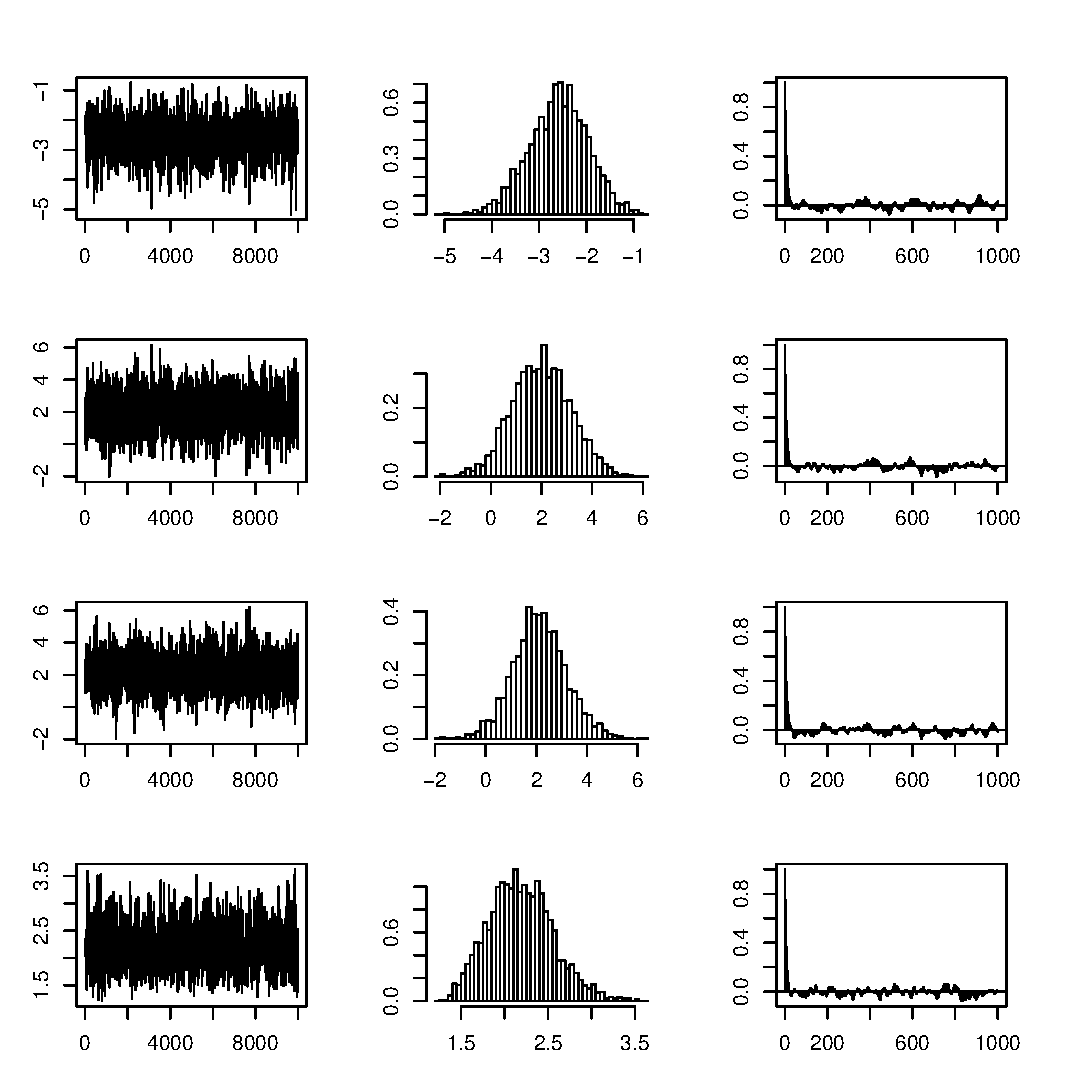
\includegraphics[width=6cm,height=5cm]{figures/hmflatlogit.eps}
\end{columns}
\small$$
\hat p_i=\frac{\exp\left(-2.5888x_{i1}+1.9967x_{i2}+2.1260x_{i3}+
2.1879x_{i4}\right)}{1+\exp\left(-2.5888x_{i1}+1.9967x_{i2}+2.1260x_{i3}+2.1879x_{i4}\right)}.
$$\normalsize

\end{slide}
\begin{frame}[fragile]
\frametitle{G-priors for logit models}

Same story: Flat prior on $\beta$ inappropriate for 
Bayes factors, to be replaced with hierarchical prior,
\small
$$
\beta|\sigma^2,X\sim\mathscr{N}_k\left(0_k,\sigma^2(X^\tee X)^{-1}\right)
\quad\text{and}\quad
\pi(\sigma^2|X)\propto \sigma^{-3/2}
$$

\begin{example}[{\sf bank}]
\begin{verbatim}
           Estimate  Post. var.  log10(BF)

X1          -2.3970   0.3286       4.8084 (****)
X2           1.6978   1.2220      -0.2453
X3           2.1197   1.0094      -0.1529
X4           2.0230   0.1132      15.9530 (****)

evidence against H0: (****) decisive, (***) strong,
(**) subtantial, (*) poor
\end{verbatim}

\end{example}
\normalsize

\end{frame}
\subsection{Loglinear models}
\begin{frame}[label=LLmdL,fragile]
\frametitle{Loglinear models}

\hyperlink{LLintro}{\beamerreturnbutton{Introduction to loglinear models}}
\begin{example}[{\sf airquality}]
Benchmark in {\sf R}\small\\
\verb&   > air=data(airquality)&\\
\normalsize
Repeated measurements over $111$ consecutive days of
ozone $u$ (in parts per billion) and maximum daily temperature $v$ 
discretized into dichotomous variables 
\footnotesize \begin{verbatim}
            month  5  6  7  8  9
 ozone    temp
 [1,31]   [57,79] 17  4  2  5 18
          (79,97]  0  2  3  3  2
 (31,168] [57,79]  6  1  0  3  1
          (79,97]  1  2 21 12  8
\end{verbatim}
\normalsize 
Contingency table with $5\times 2\times 2=20$ entries 
\end{example}

\end{frame}
\begin{slide}\slidetitle{Poisson regression}

Observations/counts $\by=(y_1,\ldots,y_n)$ are integers, so we can choose
$$
y_i\sim\mathscr{P}(\mu_i)
$$
Saturated likelihood
$$
\ell(\mu|\by)=\prod_{i=1}^n\frac{1}{\mu_i!}\mu_i^{y_i}\exp(-\mu_i)
$$

\pause
GLM constraint via log-linear link
$$
\log(\mu_i)=\bx^{i\tee}\beta\,,\quad y_i|\bx^i\sim\mathscr{P}\left(e^{\bx^{i\tee}\beta}\right)
$$

\end{slide}
\begin{slide}\slidetitle{Categorical variables}

\begin{block}{Special feature} {\em Incidence matrix} $X=(\bx^i)$ 
such that its elements are all zeros or ones, i.e.~covariates 
are all indicators/dummy variables!
\end{block}

\vs\pause
Several types of (sub)models are possible depending on relations between categorical variables.

\vs\pause
\begin{block}{Re-special feature} 
Variable selection problem of a specific kind, in the sense that all indicators related
with the {\em same} association must either remain or vanish at once. Thus
much fewer submodels than
in a regular variable selection problem.
\end{block}

\end{slide}
\begin{slide}\slidetitle{Parameterisations}

Example of three variables $1\le u\le I$, $1\le v\le j$ and $1\le w\le K$.

\vs\pause
Simplest non-constant model is
$$
\log(\mu_\tau) = \sum_{b=1}^I \beta^u_b \mathbb{I}_b(u_\tau)
               + \sum_{b=1}^J \beta^v_b \mathbb{I}_b(v_\tau)
               + \sum_{b=1}^K \beta^w_b \mathbb{I}_b(w_\tau)\,,
$$
that is,
$$
\log(\mu_{l(i,j,k)})=\beta^u_i + \beta^v_j +\beta^w_k\,,
$$
where index $l(i,j,k)$ corresponds to $u=i$, $v=j$ and $w=k$. 

\pause Saturated model is 
$$
\log(\mu_{l(i,j,k)})=\beta^{uvw}_{ijk}
$$

\end{slide}\begin{slide}\slidetitle{Log-linear model (over-)parameterisation}

Representation 
$$
\log(\mu_{l(i,j,k)})=\lambda+\lambda^u_i+\lambda^v_j+\lambda^w_k+\lambda^{uv}_{ij}
+\lambda^{uw}_{ik}+\lambda^{vw}_{jk}+\lambda^{uvw}_{ijk}\,,
$$
as in {\sf Anova} models.

\pause
\begin{itemize} 
\item $\lambda$ appears as the overall or reference average effect 
\item $\lambda^u_i$ appears as the marginal discrepancy (against the reference effect $\lambda$) when $u=i$, 
\item $\lambda^{uv}_{ij}$ as the interaction discrepancy (against the added effects $\lambda+\lambda^u_i+
	\lambda^v_j$) when $(u,v)=(i,j)$
\end{itemize}
and so on...

\end{slide}\begin{slide}\slidetitle{Example of submodels}

\small
\begin{enumerate}
\item if both $v$ and $w$ are irrelevant, then
$$
\log(\mu_{l(i,j,k)})=\lambda+\lambda^u_i\,,
$$
\item if all three categorical variables are mutually independent, then
$$
\log(\mu_{l(i,j,k)})=\lambda+\lambda^u_i+\lambda^v_j+\lambda^w_k\,,
$$
\item if $u$ and $v$ are associated but are both independent of $w$, then
$$
\log(\mu_{l(i,j,k)})=\lambda+\lambda^u_i+\lambda^v_j+\lambda^w_k+\lambda^{uv}_{ij}\,,
$$
\item if $u$ and $v$ are conditionally independent given $w$, then
$$
\log(\mu_{l(i,j,k)})=\lambda+\lambda^u_i+\lambda^v_j+\lambda^w_k+\lambda^{uw}_{ik}+\lambda^{vw}_{jk}\,,
$$
\item if there is no three-factor interaction, then
$$
\log(\mu_{l(i,j,k)})=\lambda+\lambda^u_i+\lambda^v_j+\lambda^w_k+\lambda^{uv}_{ij}+\lambda^{uw}_{ik}+\lambda^{vw}_{jk}
$$
{\em [the most complete submodel]}
\end{enumerate}
\normalsize

\end{slide}
\begin{slide}\slidetitle{Identifiability}

Representation 
$$
\log(\mu_{l(i,j,k)})=\lambda+\lambda^u_i+\lambda^v_j+\lambda^w_k+\lambda^{uv}_{ij}
+\lambda^{uw}_{ik}+\lambda^{vw}_{jk}+\lambda^{uvw}_{ijk}\,,
$$
not identifiable but Bayesian approach handles
non-identifiable settings and still estimate properly identifiable quantities. 

\pause
Customary to impose identifiability constraints
on the parameters: set to $0$ parameters corresponding to the first category of
each variable, i.e.~remove the indicator of the first category. 

\vs E.g., if $u\in\{1,2\}$ and $v\in\{1,2\}$, constraint could be
$$
\lambda^u_1=\lambda^v_1=\lambda^{uv}_{11}=\lambda^{uv}_{12}=\lambda^{uv}_{21}=0\,.
$$

\end{slide}
\begin{frame}[fragile]
\frametitle{Inference under a flat prior}

Noninformative prior $\pi(\beta)\propto 1$ gives posterior distribution
\small\begin{eqnarray*}
\pi(\beta|\by,X) &\propto& \prod_{i=1}^n\left\{\exp(\bx^{i\tee}\beta)\right\}^{y_i}\exp\{-\exp(\bx^{i\tee}\beta)\}\\
&=& \exp\left\{ \sum_{i=1}^n y_i\,\bx^{i\tee} \beta - \sum_{i=1}^n \exp (\bx^{i\tee}\beta) \right\}\\
\end{eqnarray*}

\vs\pause
Use of same random walk M-H algorithm as in probit and logit cases, starting with
MLE evaluation
\begin{verbatim}
  > mod=summary(glm(y~-1+X,family=poisson()))
\end{verbatim}

\end{frame}
\begin{slide}\slidetitle{{\sf airquality}}

\begin{columns}\column{.5\textwidth}
Identifiable non-saturated model involves $16$ parameters

Obtained with
$10,000$ MCMC iterations with scale factor $\tau^2=0.5$

\column{.5\textwidth}
\footnotesize
\begin{tabular}{l|r r}
            Effect  & Post. mean  & Post. var. \\
\hline $\lambda$     &  2.8041     & 0.0612 \\
 $\lambda^u_2$       & -1.0684     & 0.2176 \\
 $\lambda^v_2$       & -5.8652     & 1.7141 \\
 $\lambda^w_2$       & -1.4401     & 0.2735 \\
 $\lambda^w_3$       & -2.7178     & 0.7915 \\
 $\lambda^w_4$       & -1.1031     & 0.2295 \\
 $\lambda^w_5$       & -0.0036     & 0.1127 \\
 $\lambda^{uv}_{22}$ &  3.3559     & 0.4490 \\
 $\lambda^{uw}_{22}$ & -1.6242     & 1.2869 \\
 $\lambda^{uw}_{23}$ &- 0.3456     & 0.8432 \\
 $\lambda^{uw}_{24}$ & -0.2473     & 0.6658 \\
 $\lambda^{uw}_{25}$ & -1.3335     & 0.7115 \\
 $\lambda^{vw}_{22}$ &  4.5493     & 2.1997 \\
 $\lambda^{vw}_{23}$ &  6.8479     & 2.5881 \\
 $\lambda^{vw}_{24}$ &  4.6557     & 1.7201 \\
 $\lambda^{vw}_{25}$ &  3.9558     & 1.7128
\end{tabular}
\normalsize
\end{columns}

\end{slide}\begin{slide}\slidetitle{{\sf airquality}: MCMC output}

\begin{columns}\column{.5\textwidth}
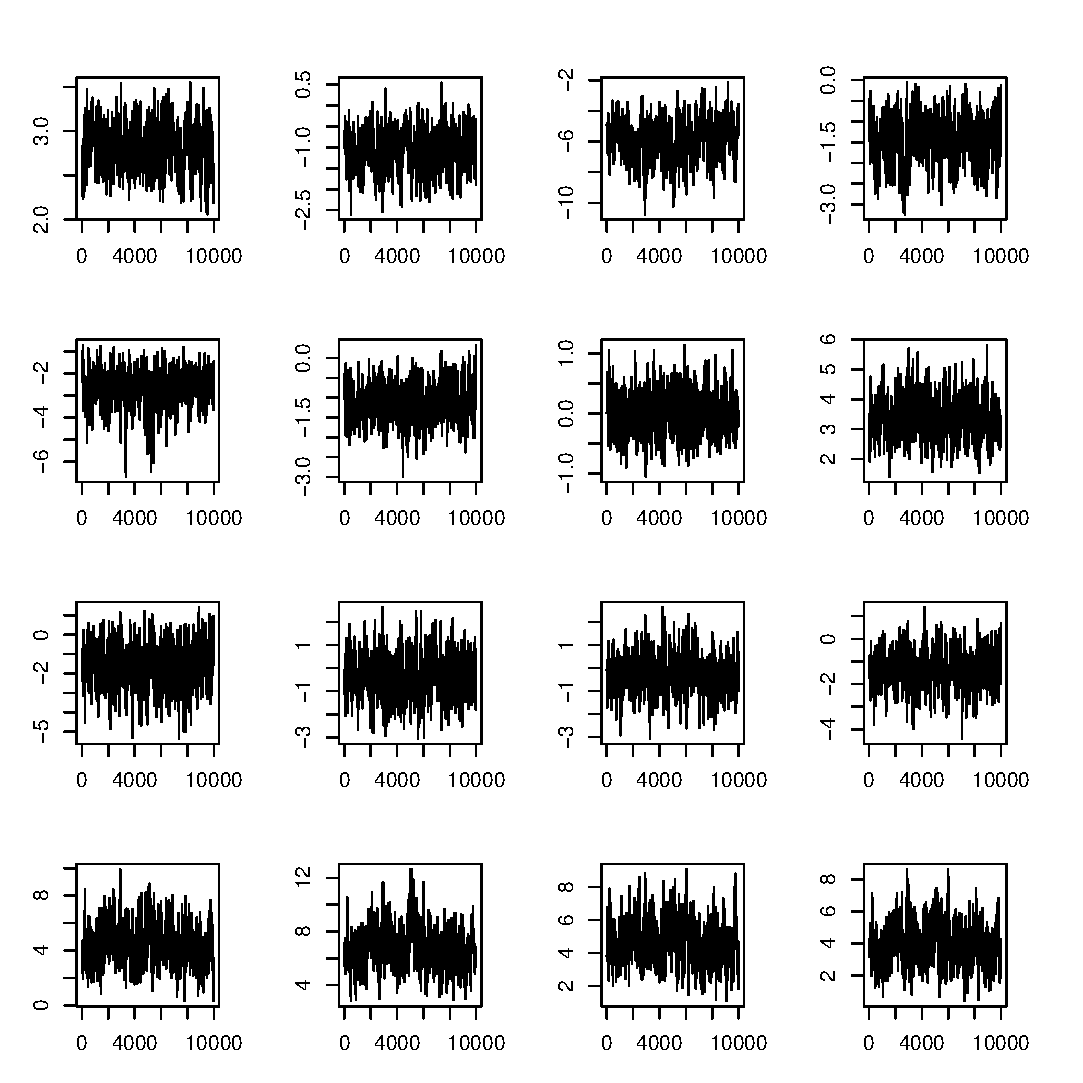
\includegraphics[width=5cm,height=6cm]{figures/trajflatloglin.eps}
\column{.5\textwidth}
\only<2>{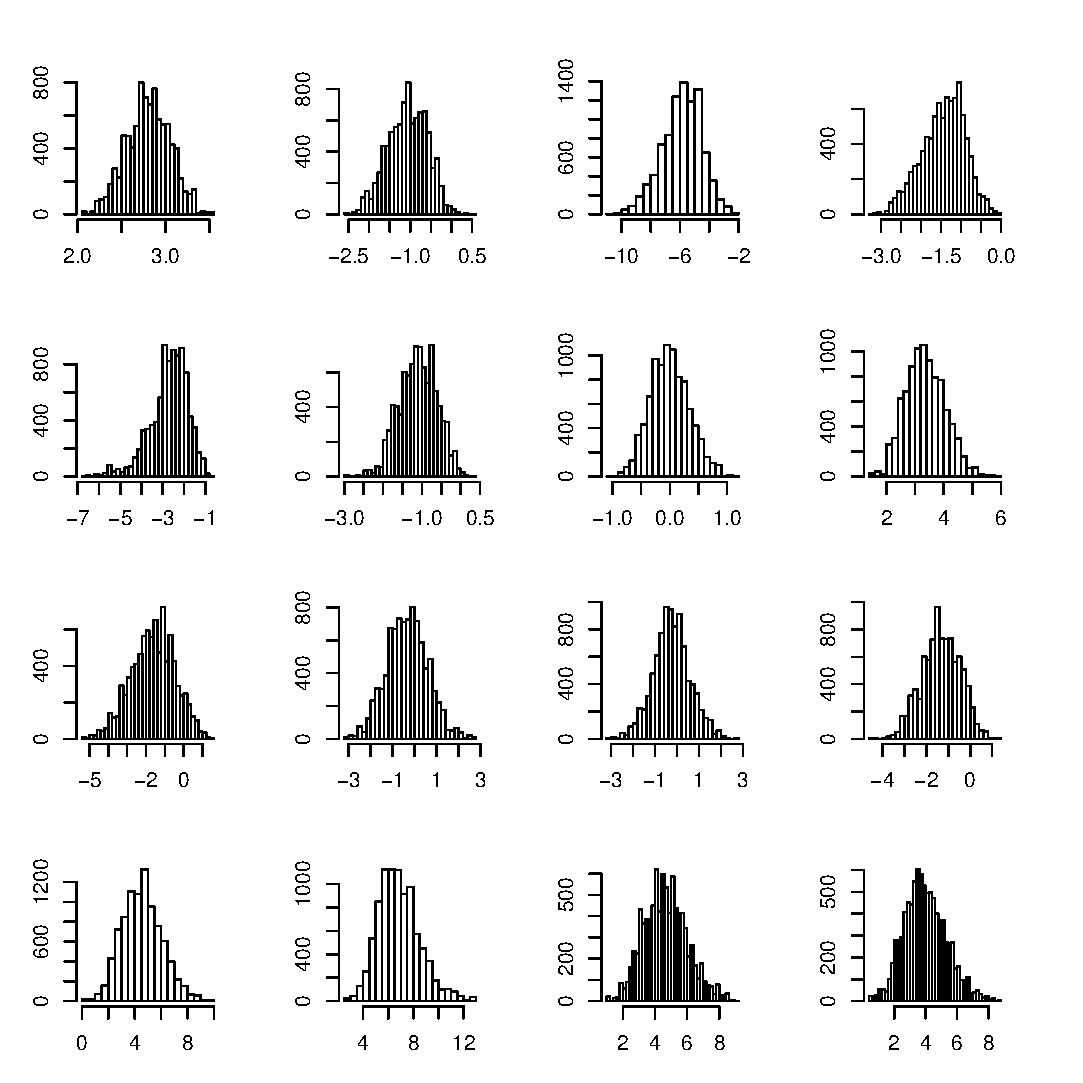
\includegraphics[width=5cm,height=6cm]{figures/histflatloglin.eps}}
\end{columns}

\end{slide}
\begin{frame}
\frametitle{Model choice with $G$-prior}

$G$-prior alternative used for probit and logit models still available:
\begin{eqnarray*}
\pi(\beta|\by,X) & \propto & |X^\tee X|^{1/2}\Gamma\left\{\frac{(2k-1)}{4}\right\}
\left|\left|X\beta\right|\right|^{-(2k-1)/2}\pi^{-k/2} \nonumber \\
&& \quad\times\exp\left\{ \left(\sum_{i=1}^n y_i\,\bx^i\right)^\tee \beta -
\sum_{i=1}^n \exp (\bx^{i\tee}\beta) \right\}
\end{eqnarray*}

\vs\pause
Same MCMC implementation and similar estimates for {\sf airquality}

\end{frame}
\begin{frame}[fragile]
\frametitle{{\sf airquality}}

Bayes factors once more approximated by importance sampling based on normal
importance functions

\vs\pause
\begin{block}{Anova-like output}
\begin{verbatim}
Effect log10(BF)

u:v     6.0983 (****)
u:w    -0.5732
v:w     6.0802 (****)

evidence against H0: (****) decisive, (***) strong,
(**) subtantial, (*) poor
\end{verbatim}
\end{block}

\end{frame}

%%%%%%%%%%%%%%%%%%%%%%%%%%%%%%%%%%%%%%%
\section{Capture-recapture experiments}
\begin{slide}\slidetitle{Capture-recapture experiments}
\tableofcontents[sectionstyle=show/hide,subsectionstyle=show/shaded/hide]

\end{slide}
%%%%%%%%%%%%%%%%%%%%%%%%%%%%%%%%%%%%%%%
\subsection{Inference in finite populations}
\begin{slide}\slidetitle{Inference in finite populations}

\normalsize 
Problem of estimating an unknown population size, $N$, based on
partial observation of this population: domain of {\em survey
sampling} 

\begin{block}{Warning}
We do not cover the official Statistics/stratified type of survey based on
a preliminary knowledge of the structure of the population
\end{block}

\end{slide}\begin{slide} 
\slidetitle{Numerous applications}

\begin{itemize}
\item \MidnightBlue{{\em Biology \&\ Ecology}} 
	for estimating the size of herds, of fish or whale populations, etc.
\pause
\item \MidnightBlue{{\em Sociology \&\ Demography}} 
	for estimating the size of populations at risk, including 
	homeless people, prostitutes, illegal migrants, drug addicts, etc.
\pause
\item \MidnightBlue{{\em official Statistics}} in the U.S.~and French census undercount procedures
\item \MidnightBlue{{\em Economics \&\ Finance}} in credit scoring, defaulting companies, etc.,
\pause
\item \MidnightBlue{{\em Fraud detection}}  phone, credit card, etc.
\item \MidnightBlue{{\em Document authentication}} historical documents, forgery, etc.,
\item \MidnightBlue{{\em Software debugging}}
\end{itemize}

\end{slide}\begin{slide} 
\slidetitle{Setup}

Size $N$ of the whole population is unknown
but samples (with fixed or random sizes) can 
be extracted from the population. 

%%%%%%%%%%%%%%%%%%%%%%%%%%%%%%%%%%%%%%%
\end{slide}\subsection{Binomial capture model}\begin{slide}
\slidetitle{The binomial capture model}

Simplest model of all: joint capture of $n^+$ individuals from a population of size $N$.

\vs\pause Population size $N\in\mathbb{N}^*$ is the parameter of interest, but there exists a
nuisance  parameter, the probability $p\in[0,1]$ of capture [under assumption of independent captures]

\vs\pause
Sampling model
$$
n^+ \sim \mathscr{B}(N,p)
$$
and corresponding likelihood 
$$
\ell(N,p|n^+)={N \choose n^+}\,p^{n^+}(1-p)^{N-n^+}\mathbb{I}_{N\ge n^+}\,.
$$

\end{slide}\begin{slide}
\slidetitle{Bayesian inference (1)}
Under vague prior
$$
\pi(N,p)\propto N^{-1}\mathbb{I}_{\mathbb{N}^*}(N)\mathbb{I}_{[0,1]}(p)\,,
$$
posterior distribution of $N$ is 
\small\begin{eqnarray*}
\pi(N|n^+) & \propto & \frac{N!}{(N-n^+)!}\,N^{-1}\mathbb{I}_{N\ge n^+}\mathbb{I}_{\mathbb{N}^*}(N)\int_0^1 p^{n^+}(1-p)^{N-n^+}dp \\
           & \propto & \frac{(N-1)!}{(N-n^+)!}\,\frac{(N-n^+)!}{(N+1)!}\,\mathbb{I}_{N\geq n^+\vee 1} \\
           & =       & \frac{1}{N(N+1)}\mathbb{I}_{N\geq n^+\vee 1}\,.
\end{eqnarray*}
\normalsize where $n^+\vee 1=\max(n^+,1)$

\end{slide}\begin{slide}
\slidetitle{Bayesian inference (2)}
If we use the uniform prior
$$
\pi(N,p)\propto \mathbb{I}_{\{1,\ldots,S\}}(N)\mathbb{I}_{[0,1]}(p)\,,
$$
the posterior distribution of $N$ is
$$
\pi(N|n^+)\propto \frac{1}{N+1}\mathbb{I}_{\{n^+\vee 1,\ldots,S\}}(N)\,.
$$

\end{slide}
\begin{slide}
\slidetitle{Capture-recapture data}

\begin{block}{European dippers}
\begin{columns}\column{.55\textwidth}
Birds closely dependent on streams, feeding on underwater invertebrates

Capture-recapture data on dippers over  years 1981--1987
in $3$ zone of $200$ $\text{km}^2$ in eastern France with markings and recaptures
of breeding adults each year, during the breeding period from early March to early June.
\column{.35\textwidth}

\includegraphics[width=3cm,height=3truecm]{figures/Dipper.eps}
\end{columns}
\end{block}

\end{slide}
\begin{frame}[fragile]
\frametitle{{\sf eurodip}}

Each row of $7$ digits corresponds to a capture-recapture story: 
$0$ stands for absence of capture and, else,
$1,2$ or $3$ represents the zone of capture.

\vs\pause
E.g.
\begin{verbatim}
1 0 0 0 0 0 0
1 3 0 0 0 0 0
0 2 2 2 1 2 2
\end{verbatim}
means: first dipper only captured the first year [in zone 1], second dipper
captured in years 1981--1982 and moved from zone 1 to zone 3 between those years, third dipper
captured in years 1982--1987 in zone 2

\end{frame}
%%%%%%%%%%%%%%%%%%%%%%%%%%%%%%%%%%%%%%%
\subsection{Two-stage capture-recapture}\begin{slide}
\slidetitle{The two-stage capture-recapture experiment}

Extension to the above with two capture periods plus a marking stage:
\begin{enumerate}
\item  $n_1$ individuals from a population of size $N$ captured {\em [sampled without replacement]}
\item  captured individuals marked and released
\item  $n_2$ individuals captured during second identical sampling experiment
\item  $m_2$ individuals out of the $n_2$'s bear the identification mark {\em [captured twice]}
\end{enumerate}

\end{slide}\begin{slide}
\slidetitle{The two-stage capture-recapture model}

For {\em closed populations} [fixed population size $N$ throughout
experiment, constant capture probability $p$ for all individuals, and independence between
individuals/captures], binomial models:
\pause
$$
n_1     \sim\mathscr{B}(N,p)\,,\quad
m_2|n_1 \sim\mathscr{B}(n_1,p)\quad\hbox{and}
$$
$$
n_2-m_2|n_1,m_2 \sim\mathscr{B}(N-n_1,p)\,.
$$

\end{slide}\begin{slide}
\slidetitle{The two-stage capture-recapture likelihood}

Corresponding likelihood $\ell(N,p|n_1,n_2,m_2)$
\small\begin{align*}
{N-n_1 \choose n_2-m_2} &p^{n_2-m_2}(1-p)^{N-n_1-n_2+m_2} \mathbb{I}_{\{0,\ldots,N-n_1\}}(n_2-m_2)\\
                      &\times  {n_1 \choose m_2}p^{m_2}(1-p)^{n_1-m_2}{N \choose n_1}p^{n_1}(1-p)^{N-n_1} \mathbb{I}_{\{0,\ldots,N\}}(n_1) \\
                      &\propto \frac{N!}{(N-n_1-n_2+m_2)!} p^{n_1+n_2}(1-p)^{2N-n_1-n_2}\mathbb{I}_{N\geq n^+} \\
                      &\propto {N \choose n^+}p^{n^c}(1-p)^{2N-n^c}\mathbb{I}_{N\geq n^+}
\end{align*}
\normalsize where $n^c=n_1+n_2$ and $n^+=n_1+(n_2-m_2)$ are
total number of captures/captured individuals over both periods 

\end{slide}\begin{slide}
\slidetitle{Bayesian inference (1)}

Under prior $\pi(N,p)=\pi(N)\pi(p)$ where $\pi(p)$ is  $\mathscr{U}([0,1])$, 
conditional posterior distribution on $p$ is
$$
\pi(p|N,n_1,n_2,m_2)=\pi(p|N,n^c)\propto p^{n^c}(1-p)^{2N-n^c}\,,
$$
that is,
$$
p|N,n^c\sim\mathscr{B}e(n^c+1,2N-n^c+1).
$$

\vs\pause
Marginal posterior distribution of $N$ more complicated. 
If $\pi(N)=\mathbb{I}_{\mathbb{N}^*}(N)$, 
$$
\pi(N|n_1,n_2,m_2)\propto {N \choose n^+}B(n^c+1,2N-n^c+1)\mathbb{I}_{N\geq n^+\vee 1}
$$
{\em [Beta-Pascal distribution]}

\end{slide}\begin{slide}
\slidetitle{Bayesian inference (2)}

Same problem if $\pi(N)=N^{-1}\mathbb{I}_{\mathbb{N}^*}(N)$. 

\begin{block}{Computations}
Since $N\in\mathbb{N}$, always possible to approximate the missing
normalizing factor in $\pi(N|n_1,n_2,m_2)$ by summing in $N$. 

Approximation errors become a problem when $N$ and $n^+$ are large.
\end{block}

\vs\pause
Under proper uniform prior,
$$
\pi(N)\propto \mathbb{I}_{\{1,\ldots,S\}}(N)\,,
$$
posterior distribution of $N$ proportional to
$$
\pi(N|n^+)\propto {N \choose n^+}\frac{\Gamma(2N-n^c+1)}{\Gamma(2N+2)}\,\mathbb{I}_{\{n^+\vee 1,\ldots,S\}}(N)\,.
$$
and can be computed with no approximation error.

\end{slide}\begin{slide}
\slidetitle{The Darroch model}

Simpler version of the above: conditional on both samples sizes $n_1$ and $n_2$,
$$
m_2|n_1,n_2 \sim \mathscr{H}(N,n_2,n_1/N)\,.
$$

Under uniform prior on $N\sim\mathscr{U}(\{1,\ldots,S\})$,
posterior distribution of $N$
$$
\pi(N|m_2) \propto {n_1 \choose m_2} {N-n_1\choose n_2-m_2} \bigg/ {N\choose n_2}\mathbb{I}_{\{n^+\vee 1,\ldots,S\}}(N)
$$
and posterior expectations computed numerically by simple summations.
\end{slide}\begin{slide}
\slidetitle{{\sf eurodip}}

For the two first years and $S=400$,
posterior distribution of $N$
for the Darroch model given by
$$
\pi(N|m_2) \propto (n-n_1)!(N-n_2)!\big/\{(n-n_1-n_2+m_2)!N!\}\,\mathbb{I}_{\{71,\ldots,400\}}(N)\,,
$$
with inverse normalization factor 
$$
\sum_{k=71}^{400} (k-n_1)!(k-n_2)!\big/\{(k-n_1-n_2+m_2)!k!\}\,.
$$

\pause Influence of prior hyperparameter $S$ (for $m_2=11$):

\small
\begin{center}\begin{tabular}{ c|c c c c c c c c c }
%\hline
$S$ & $100$ & $150$ & $200$ & $250$ & $300$ & $350$ & $400$ & $450$ & $500$ \cr
\hline
$\mathbb{E}[N|m_2]$ & $95$ & $125$ & $141$ & $148$  & $151$ & $151$ & $152$ & $152$ & $152$ \cr
%\hline
\end{tabular}\end{center}
\normalsize

\end{slide}\begin{slide}
\slidetitle{Gibbs sampler for $2$-stage capture-recapture}

If $n^+>0$, both conditional posterior distributions are standard, since
\begin{eqnarray*}
p|n^c,N      & \sim & \mathscr{B}e(n^c+1,2N-n^c+1) \\
N-n^+|n^+,p  & \sim & \mathscr{N}eg(n^+,1-(1-p)^2)\,.
\end{eqnarray*}

Therefore, joint distribution of $(N,p)$ can be approximated by a Gibbs sampler

%%%%%%%%%%%%%%%%%%%%%%%%%%%%%%%%%%%%%%%
\end{slide}\begin{slide}
\slidetitle{$T$-stage capture-recapture model}

Further extension to the two-stage capture-recapture model: series of $T$ consecutive captures.

$n_t$ individuals captured at period $1\le t\le T$, and $m_t$ recaptured individuals (with the convention that $m_1=0$) 
$$
n_1\sim\mathscr{B}(N,p)
$$
and, conditional on earlier captures/recaptures $(2\le j\le T)$,
\begin{align*}
m_j&\sim\mathscr{B}\left(\sum_{t=1}^{j-1}(n_t-m_t),p\right)\quad\hbox{and}\\
n_j-m_j&\sim\mathscr{B}\left(N-\sum_{t=1}^{j-1}(n_t-m_t),p\right)\,.
\end{align*}

\end{slide}\begin{slide}
\slidetitle{$T$-stage capture-recapture likelihood}

Likelihood $\ell(N,p|n_1,n_2,m_2\ldots,n_T,m_T)$ given by
\small\begin{align*}
{N \choose n_1} & p^{n_1}(1-p)^{N-n_1} \prod_{j=2}^T\left[{N-{\sum_{t=1}^{j-1}}(n_t-m_t) 
\choose n_j-m_j}\right. p^{n_j-m_j}\\
& \times (1-p)^{N-{\sum_{t=1}^{j}}(n_t-m_t)} \left.{{\sum_{t=1}^{j-1}}(n_t-m_t) \choose m_j}\right. \\
& \times \left.p^{m_j}(1-p)^{{\sum_{t=1}^{j-1}}(n_t-m_t)-m_j}\right]\,.
\end{align*}
\normalsize

\end{slide}\begin{slide}
\slidetitle{Sufficient statistics}

Simplifies into
$$
\ell(N,p|n_1,n_2,m_2\ldots,n_T,m_T) \propto \frac{N!}{(N-n^+)!}p^{n^c}(1-p)^{TN-n^c}\mathbb{I}_{N\geq n^+}
$$
with the sufficient statistics 
$$
n^+=\sum_{t=1}^{T}(n_t-m_t)
\quad\hbox{and}\quad
n^c=\sum_{t=1}^Tn_t\,,
$$
total number of captured individuals/captures over the $T$ periods

\end{slide}\begin{slide}
\slidetitle{Bayesian inference (1)}

Under noninformative prior $\pi(N,p) = 1/N$, joint posterior 
\small\begin{eqnarray*}
\pi(N,p|n^+,n^c) & \propto & \frac{(N-1)!}{(N-n^+)!}\, p^{n^c} (1-p)^{TN-n^c}\mathbb{I}_{N\geq n^+\vee 1}\,.
\end{eqnarray*}\normalsize
leads to conditional posterior
\small$$
p|N,n^+,n^c \sim \mathscr{B}e(n^c+1,TN-n^c+1)
$$\normalsize
and marginal posterior 
\small$$
\pi(N|n^+,n^c) \propto {(N-1)! \over (N-n^+)!}\, { (TN-n^c)! \over (TN+1)!}\, \mathbb{I}_{N\ge n^+\vee 1}
$$\normalsize
which is computable {\em [under previous provisions]}.

\vs\pause
Alternative Gibbs sampler also available.
\end{slide}\begin{slide}
\slidetitle{Bayesian inference (2)}

Under prior $N\sim\mathscr{U}(\{1,\ldots,S\})$ and $p\sim\mathscr{U}([0,1])$,
$$
\pi(N|n^+)\propto {N \choose n^+}\,\frac{(TN-n^c)!}{(TN+1)!}\,\mathbb{I}_{\{n^+\vee 1,\ldots,S\}}(N).
$$

\pause\begin{block}{{\sf eurodip}}
For the whole set of observations, $T=7$, $n^+=294$ and  $n^c=519$.

For $S=400$, the posterior expectation of $N$ is equal to $372.89$.

For $S=2500$, it is $373.99$.
\end{block}

\end{slide}\begin{slide} 
\slidetitle{Computational difficulties}

E.g., heterogeneous capture--recapture 
model where individuals are captured at time $1\le t\le T$ with 
probability $p_t$ with both $N$ and the $p_t$'s are unknown. 

\vs\pause
Corresponding likelihood
\begin{align*}
\ell(N,p_1, \ldots,p_T&|n_1,n_2,m_2\ldots,n_T,m_T)\\
&\propto {N!\over (N - n^+)!} \; 
\prod_{t=1}^{T} \; p_{t}^{n_{t}} (1 - p_{t})^{N-n_{t}}.
\end{align*}

\end{slide}\begin{slide}
\slidetitle{Computational difficulties (cont'd)}

Associated prior $N \sim\mathscr{P}(\lambda)$ and
$$
\alpha_{t} = \log \left({p_{t}\big/ 1 - p_{t}}\right)
\sim {\mathscr{N}}(\mu_{t},\sigma^{2}),
$$
where the $\mu_t$'s and $\sigma$ are known.

\pause
Posterior 
\small\begin{eqnarray*}
\pi(\alpha_1,\ldots,\alpha_T,N|,n_1,\ldots,n_T) \; & \propto & {N!\over (N - n^+)!}\,\frac{\lambda^N}{N!}
\; \prod_{t=1}^T (1 + e^{\alpha_{t}})^{-N} \\
&& \times \prod_{t=1}^T \; \exp \left\{\alpha_t n_t
- {1\over 2\sigma^2 } (\alpha_{t} - \mu_{t})^{2} \right\} \,.
\end{eqnarray*}\normalsize
much less manageable computationally. 

%%%%%%%%%%%%%%%%%%%%%%%%%%%%%%%%%%%%%%%
\end{slide}\subsection{Open population}\begin{slide}
\slidetitle{Open populations}

More realistically, population size does not remain fixed over time: 
probability $q$ for each individual to leave the population at each time [or between
each capture episode] 

\vs\pause
First occurrence of missing variable model.

\vs\pause
Simplified version
where only individuals captured during the first experiment are marked and 
their subsequent recaptures are registered.

\end{slide}\begin{slide}
\slidetitle{Working example}

Three successive capture experiments with
\small\begin{align*}
n_1&\sim\mathscr{B}(N,p),\\
r_1|n_1&\sim\mathscr{B}(n_1,q),\\
c_2|n_1,r_1&\sim\mathscr{B}(n_1-r_1,p),\\ 
r_2|n_1,r_1&\sim\mathscr{B}(n_1-r_1,q)\\
c_3|n_1,r_1,r_2&\sim\mathscr{B}(n_1-r_1-r_2,p)
\end{align*}\normalsize
where only $n_1$, $c_2$ and $c_3$ are observed. 

\vs Variables $r_1$ and $r_2$ not available and therefore part of unknowns like
parameters $N$, $p$ and $q$.

\end{slide}\begin{slide}
\slidetitle{Bayesian inference}
Likelihood 
\small
\begin{align*}
{N\choose n_1}&p^{n_1}(1-p)^{N-n_1}\,{n_1\choose r_1}\,q^{r_1}(1-q)^{n_1-r_1}{n_1-r_1\choose c_2}\,p^{c_2}(1-p)^{n_1-r_1-c_2}\\
&{n_1-r_1\choose r_2} q^{r_2}(1-q)^{n_1-r_1-r_2}{n_1-r_1-r_2\choose c_3} p^{c_3}(1-p)^{n_1-r_1-r_2-c_3}
\end{align*}\normalsize
and prior 
$$
\pi(N,p,q)=N^{-1}\mathbb{I}_{[0,1]}(p)\mathbb{I}_{[0,1]}(q)
$$

\end{slide}\begin{slide}
\slidetitle{Full conditionals for Gibbs sampling}

\begin{align*}
\pi(p|N,q,\mathcal{D}^*) &\propto p^{n_+} (1-p)^{u_+}\\
\pi(q|N,p,\mathcal{D}^*) &\propto q^{c_1+c_2}(1-q)^{2n_1-2r_1-r_2}\\
\pi(N|p,q,\mathcal{D}^*) &\propto {(N-1)! \over (N-n_1)!} (1-p)^N \mathbb{I}_{N\ge n_1}\\
\pi(r_1|p,q,n_1,c_2,c_3,r_2) &\propto \frac{(n_1-r_1)!\,q^{r_1}(1-q)^{-2r_1}(1-p)^{-2r_1}}{
        r_1!(n_1-r_1-r_2-c_3)!(n_1-c_2-r_1)!}\\
\pi(r_2|p,q,n_1,c_2,c_3,r_1) &\propto \frac{q^{r_2}[(1-p)(1-q)]^{-r_2}}{
        r_2!(n_1-r_1-r_2-c_3)!}
\end{align*}
where 
\small
\begin{align*}
\mathcal{D}^*&=(n_1,c_2,c_3,r_1,r_2)\\
u_1&=N-n_1,\,u_2=n_1-r_1-c_2,\,u_3=n_1-r_1-r_2-c_3\\
n_+&=n_1+c_2+c_3,\,u_+=u_1+u_2+u_3
\end{align*}

\end{slide}\begin{slide}
\slidetitle{Full conditionals (2)}
\normalsize
Therefore,
\begin{align*}
p|N,q,\mathcal{D}^* &\sim \mathcal{B}e(n_++1, u_++1) \\
q|N,p,\mathcal{D}^* &\sim \mathcal{B}e(r_1+r_2+1, 2n_1-2r_1-r_2+1) \\
N-n_1|p,q,\mathcal{D}^* &\sim \mathcal{N}eg(n_1,p)\\
%m_1|p,q,n_1,n_2,n_3&\sim \mathcal{B}\left(n_1-m_2-n_3,\frac{q}{1+(1-q)(1-p)^2}\right)
r_2|p,q,n_1,c_2,c_3,r_1 &\sim \mathcal{B}\left(n_1-r_1-c_3,\frac{q}{1+(1-q)(1-p)}\right)
\end{align*}

\vs\pause
$r_1$ has a less conventional distribution,  but, since $n_1$ not
extremely large, possible to compute the probability that $r_1$ is equal 
to one of the values in $\{0,1,\ldots,\min(n_1-r_2-c_3,n_1-c_2)\}$.

\end{slide}\begin{slide}
\slidetitle{{\sf eurodip}}

\begin{columns}
\column{.5\textwidth}
$n_1=22$, $c_2=11$ and $c_3=6$

MCMC approximations to the posterior expectations
of $N$ and $p$ equal to 57 and 0.40

\column{.5\textwidth}
\only<1>{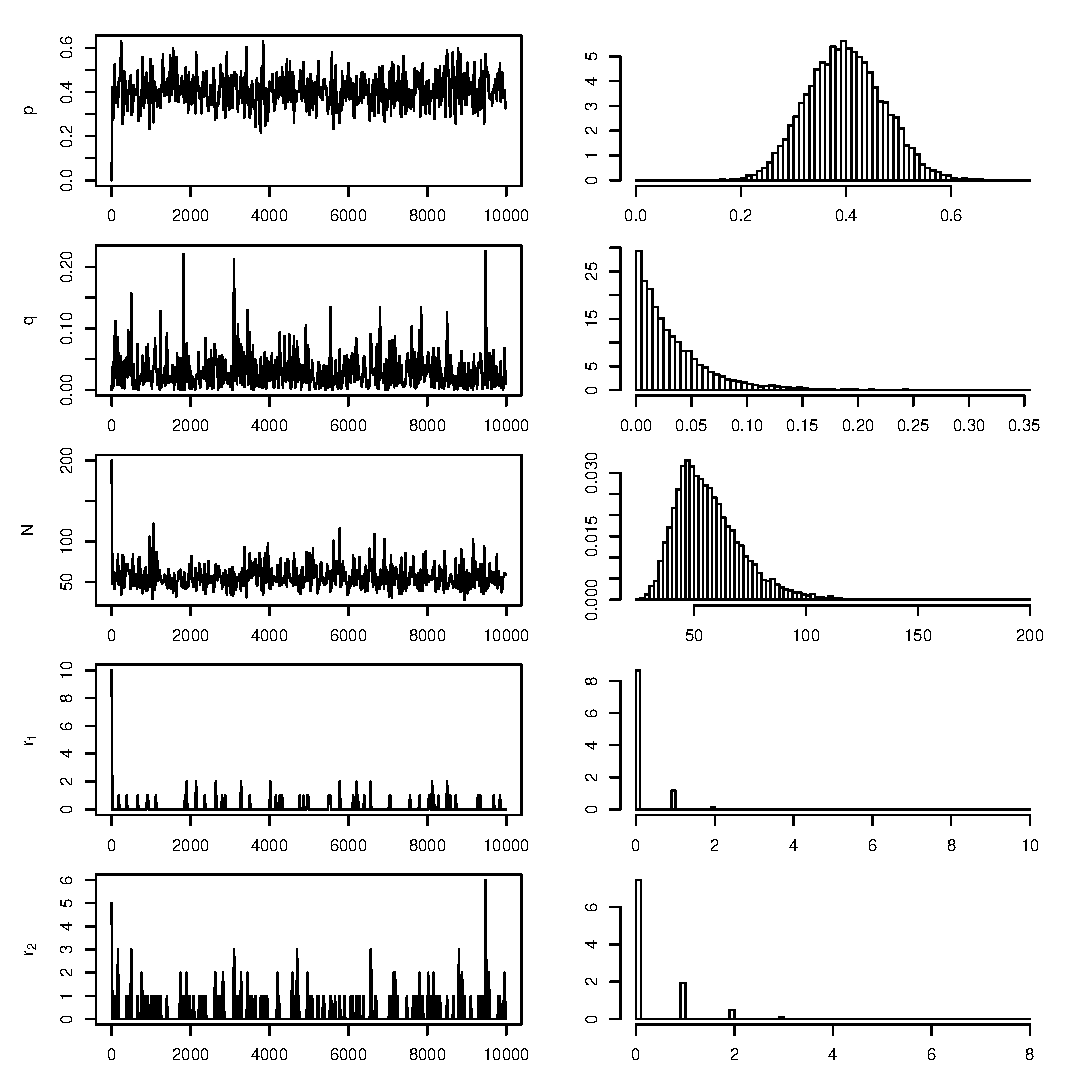
\includegraphics[width=4truecm,height=6truecm]{figures/g2.eps}}
%\only<2>{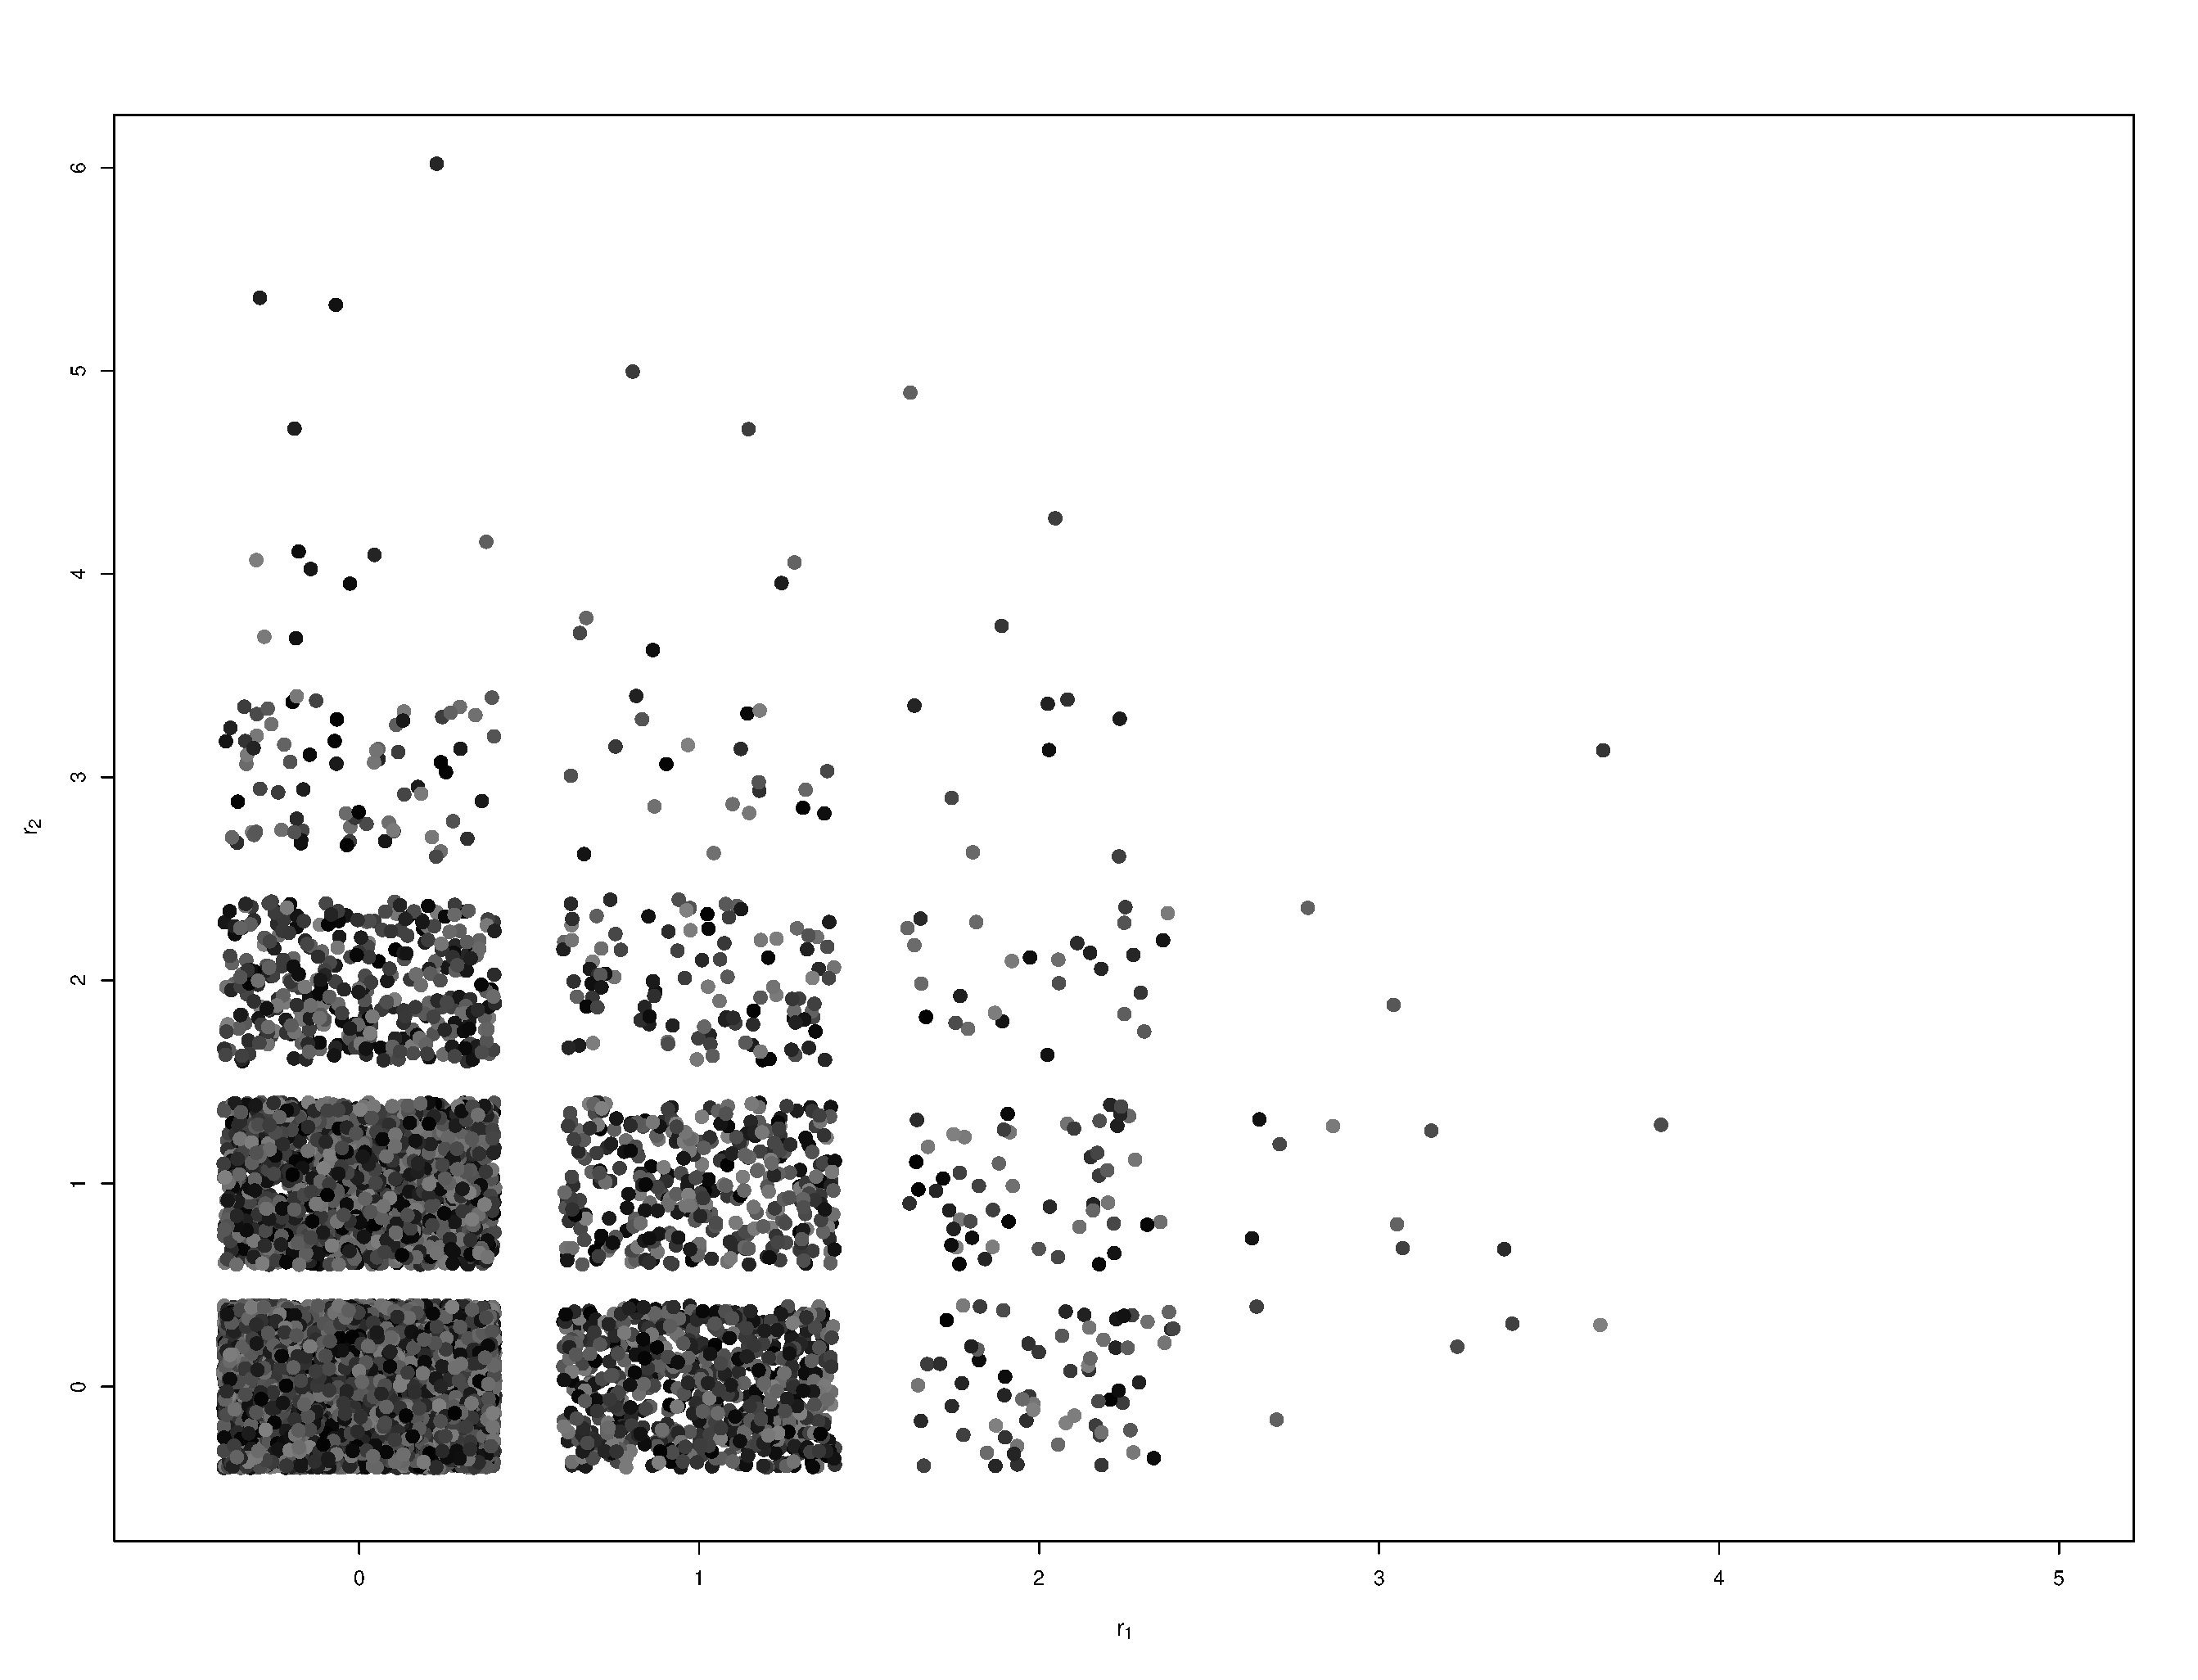
\includegraphics[width=4truecm,height=6truecm]{figures/jit.eps}}
\end{columns}

\end{slide}\begin{slide}
\slidetitle{{\sf eurodip}}

\begin{columns}
\column{.5\textwidth}
$n_1=22$, $c_2=11$ and $c_3=6$

MCMC approximations to the posterior expectations
of $N$ and $p$ equal to 57 and 0.40

\column{.5\textwidth}
%\only<1>{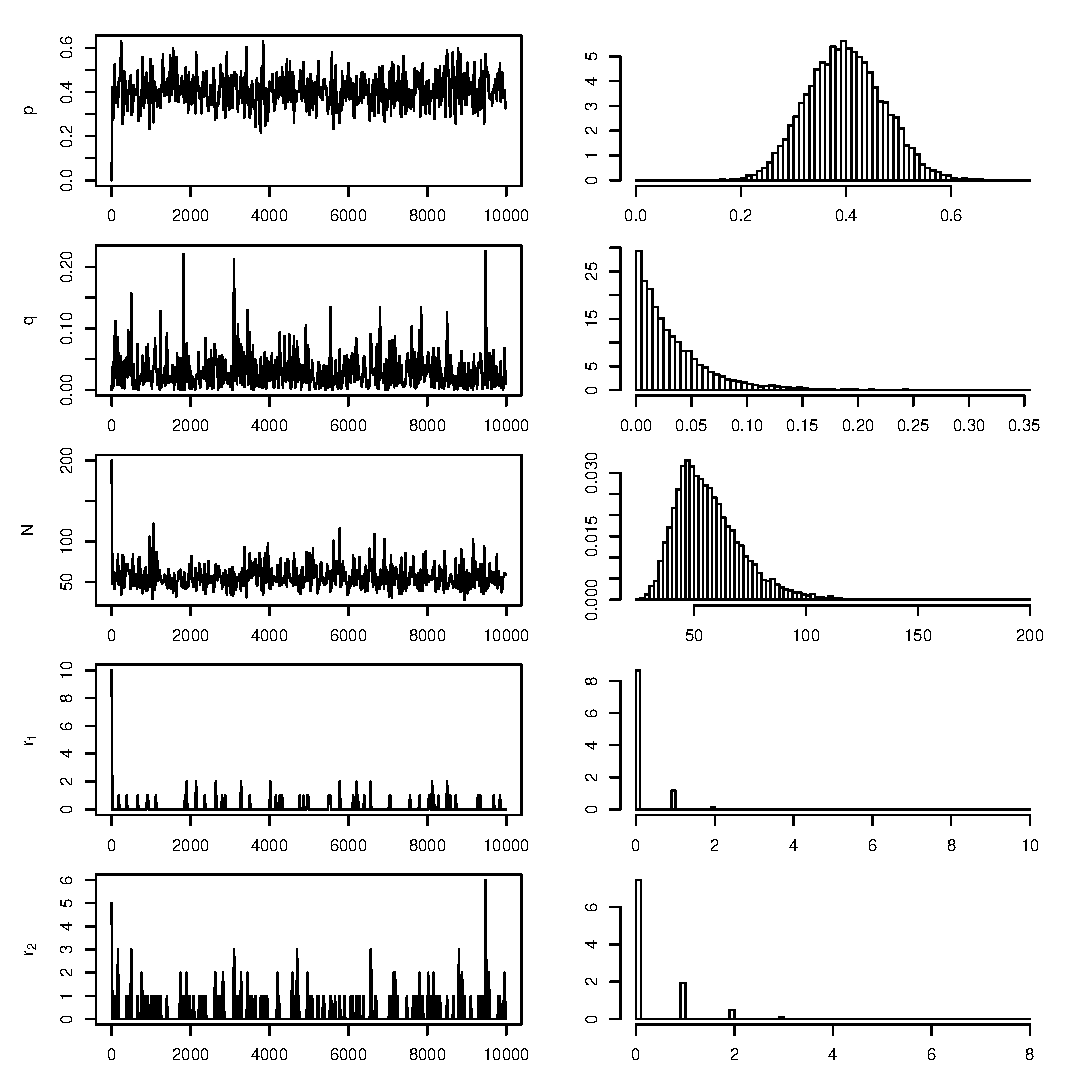
\includegraphics[width=4truecm,height=6truecm]{figures/g2.eps}}
\only<1>{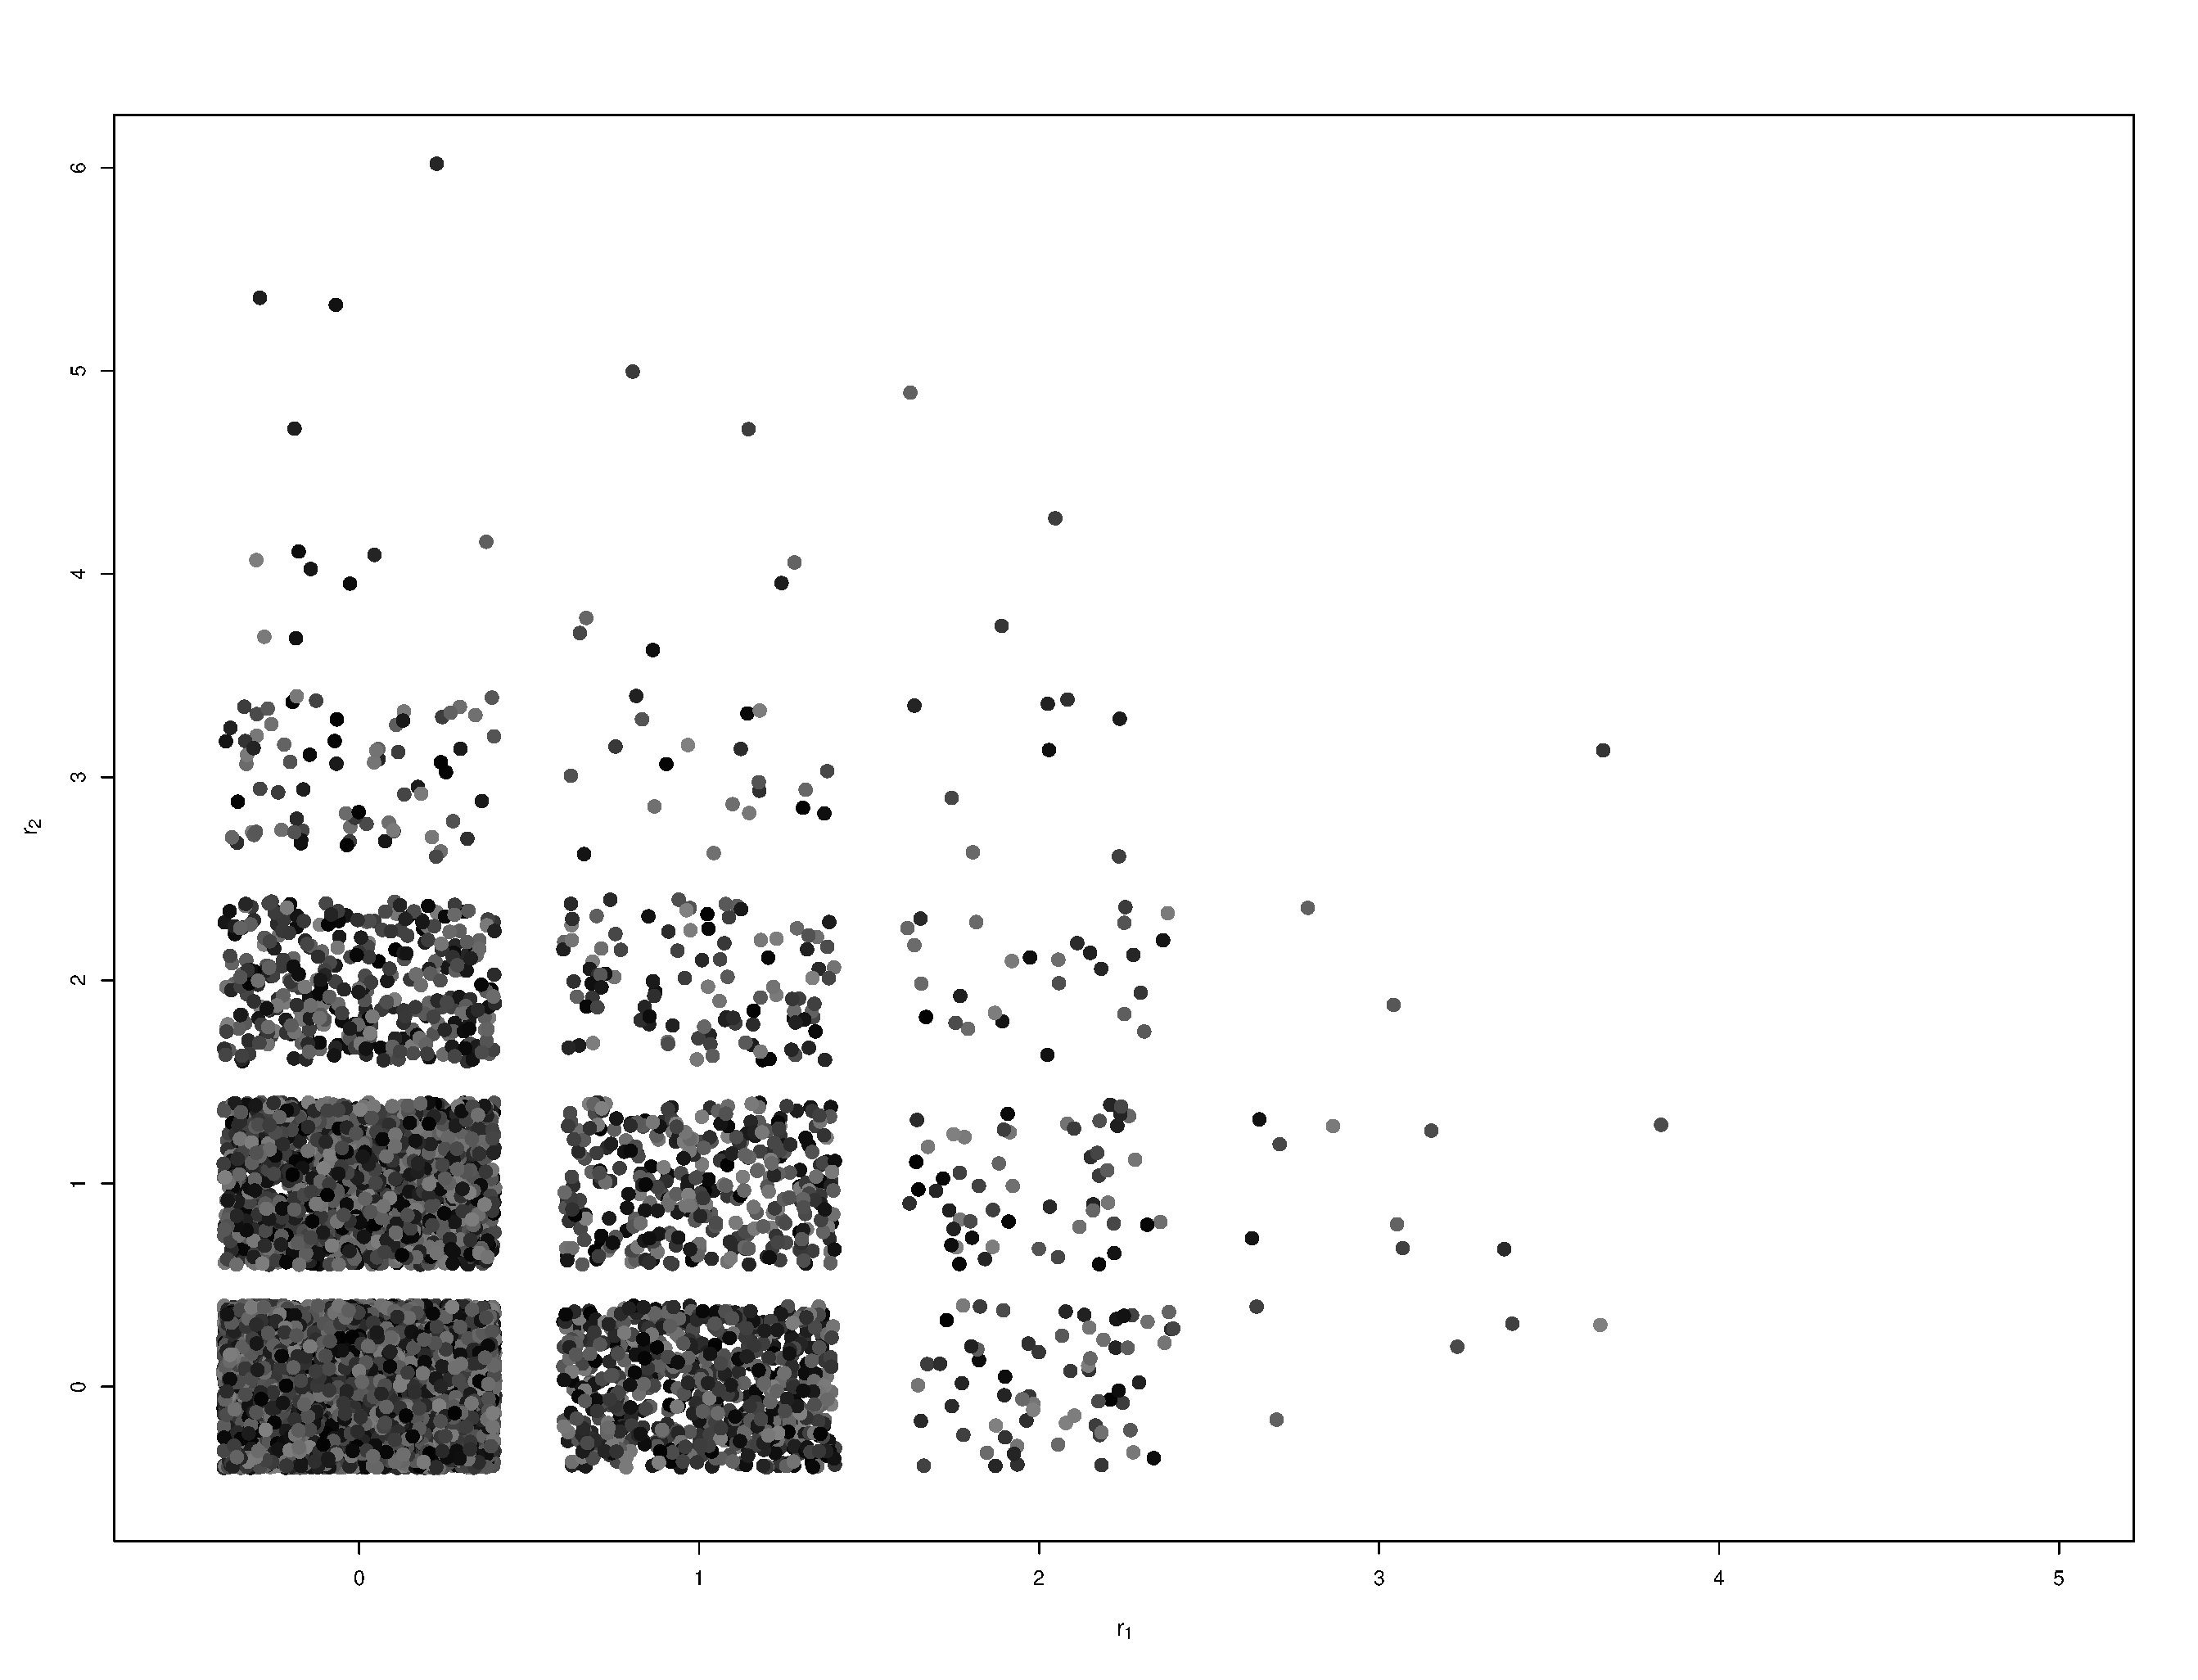
\includegraphics[width=4truecm,height=6truecm]{figures/jit.eps}}
\end{columns}

%%%%%%%%%%%%%%%%%%%%%%%%%%%%%%%%%%%%%%%
\end{slide}\subsection{Accept-Reject methods}\begin{slide}
\slidetitle{Accept-Reject methods}

\begin{itemize}
\item Many distributions from which it is difficult, or even impossible,
to directly simulate.

\item Technique that only
require us to know the functional form of the target
$\pi$ of interest up to a multiplicative constant.

\item Key to this method is to use a proposal density $g$
{\em [as in Metropolis-Hastings]}
\end{itemize}

\end{slide}\begin{slide}
\slidetitle{Principle}

Given a target density $\pi$, find a density $g$ and a constant $M$ such that
$$
\pi(x) \leq M g(x)
$$
on the support of $\pi$.

\vs\pause
Accept-Reject algorithm is then
{\Brown{\tt
\colorbox{LightGrey}{\makebox[0.9\textwidth][c]{\parbox{0.85\textwidth}{
\begin{enumerate}
\item Generate $X \sim g$, $U\sim {\cal{U}}_{[0,1]}$ ;
\item Accept $Y = X$ if $U \leq \frac{f(X) }{ Mg(X)}$ ; 
\item Return to 1.\  otherwise. 
\end{enumerate}
}}}}}

\end{slide}\begin{slide}
\slidetitle{Validation of Accept-Reject}

This algorithm produces a variable $Y$\\ distributed according to $f$

\begin{block}{Fundamental theorem of simulation}
\begin{columns}
\column{.65\textwidth}
Simulating
$$
X \sim f(x)
$$
is equivalent to simulating
$$
(X,U) \sim {\mathcal U} \{(x,u):0<u<\pi(x)\}
$$
\column{.3\textwidth}
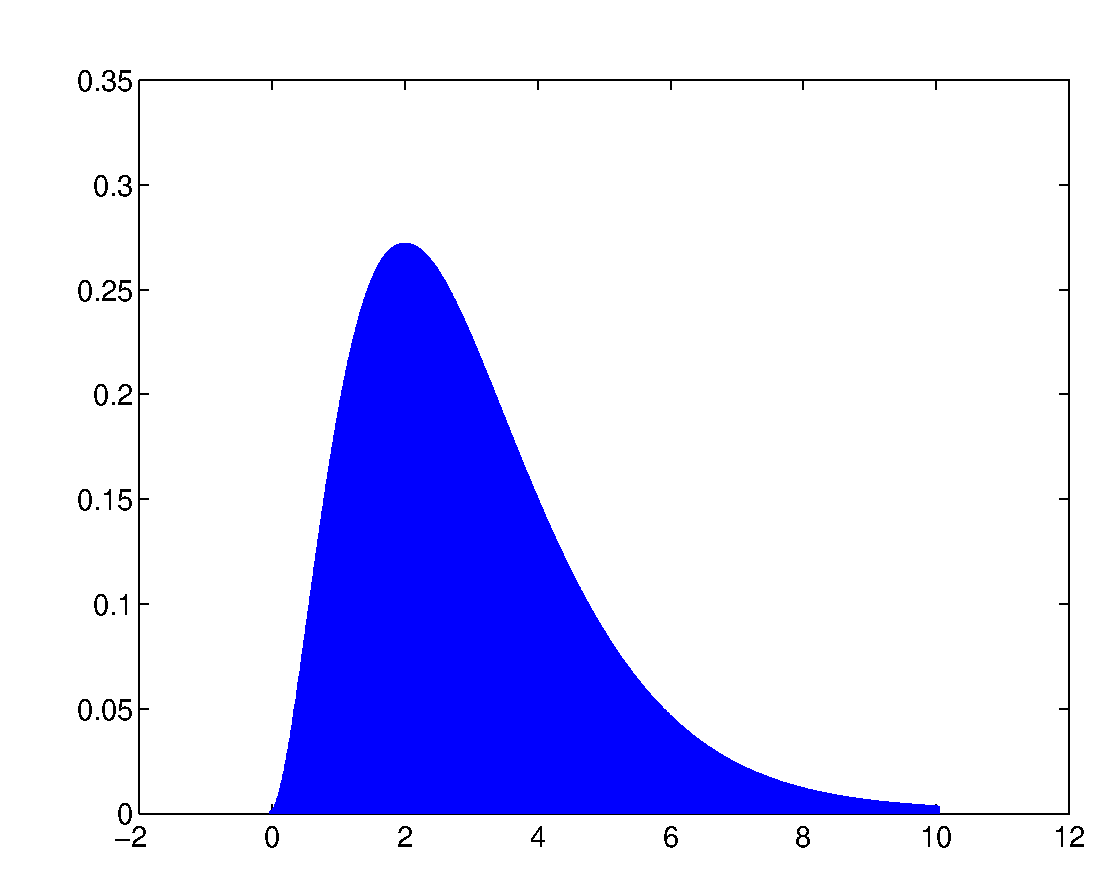
\includegraphics[width=3cm]{figures/uniform.eps}
\end{columns}
\end{block}

\end{slide}\begin{slide}
\slidetitle{Two interesting properties:}

\begin{enumerate}
\item[$\circ$] First, Accept-Reject provides a generic method 
to simulate from any density $\pi$ that is known {\it up to a multiplicative factor}

Particularly important for Bayesian calculations since
$$
  \pi(\theta|x) \propto \pi(\theta) \; f(x|\theta) \;. 
$$
is specified up to a normalizing constant
\pause
\item[$\circ$] Second, the probability of acceptance in the algorithm is $1/M$, e.g.,
expected number of trials until a variable is accepted is $M$
\end{enumerate}

\end{slide}\begin{slide}
\slidetitle{Application to the open population model}

Since full conditional distribution of $r_1$ non-standard,
rather than using exhaustive enumeration of all
probabilities $\mathbb{P}(m_1=k)=\pi(k)$ and then sampling from this distribution,
try to use a proposal based on a binomial upper bound. 

\vs\pause
Take $g$ equal to the binomial $\mathscr{B}(n_1,q_1)$ with 
$$
q_1=q/(1-q)^2(1-p)^2
$$

\end{slide}\begin{slide}
\slidetitle{Proposal bound}

$\pi(k)/g(k)$ proportional to
\footnotesize
$$
\frac{{n_1-c_2\choose k} (1-q_1)^k {n_1-k\choose r_2+c_3}}
{{n_1\choose k}} = \frac{(n_1-c_2)!}{(r_2+c_3)!n_1!}\,
\frac{((n_1-k)!)^2(1-q_1)^k}{(n_1-c_2-k)!(n_1-r_2-c_3-k)!}
$$\normalsize
decreasing in $k$, therefore bounded by
\small$$
\frac{(n_1-c_2)!}{(r_2+c_3)!}\,
\frac{n_1!}{(n_1-c_2)!(n_1-r_2-c_3)!}={n_1\choose r_2+c_3}\,.
$$\normalsize

\pause
\begin{itemize}
\item[$\lightning$] This is {\em not} the constant $M$ because of unnormalised 
densities [$M$ may also depend on $q_1$]. Therefore the average acceptance rate 
is undetermined and requires an extra Monte Carlo experiment
\end{itemize}

\end{slide}
%%%%%%%%%%%%%%%%%%%%%%%%%%%%%%%%%%%%%%%%%%%%%%%%%%%%%%%%%%%%%%%%%%%%%
\subsection{Arnason--Schwarz's Model}
\begin{slide}\slidetitle{Arnason--Schwarz Model}

\begin{columns}
\column{.55\textwidth}
Representation of a capture recapture experiment as a collection of individual histories:
for each individual captured at least once, individual characteristics
of interest (location, weight, social status, \&tc.) registered at each capture. 
\column{.4\textwidth}
\includegraphics[width=3truecm,angle=270]{figures/titlcap.eps}
\end{columns}

\vs\pause Possibility that individuals vanish from the {\em [open]} population 
between two capture experiments.

\end{slide}\begin{slide}
\slidetitle{Parameters of interest}

Study the movements of individuals between zones/strata rather than estimating
population size.

\vs\pause
Two types of variables associated with each individual $i=1,\ldots,n$

\begin{enumerate}
\item a variable for its location {\em [partly observed]},
$$
\mathbf{z}_i =(z_{(i,t)},t=1,..,\tau)
$$
where $\tau$ is the number of capture periods, 
\item a binary variable for its capture history {\em [completely observed]},
$$
\mathbf{x}_i=(x_{(i,t)},t=1,..,\tau)\,.
$$
\end{enumerate}

\end{slide}\begin{slide}
\slidetitle{Migration \&\ deaths}

$z_{(i,t)}=r$ when individual $i$ is alive in stratum $r$ at time $t$ 
and denote $z_{(i,t)}=\dag$ for the case when it is dead at time $t$.

\vs\pause Variable $\mathbf{z}_i$ sometimes called {\em migration} process of
individual $i$ as when animals moving between geographical zones.

\vs\pause
E.g., 
$$
{\mathbf x}_i = 1 \; 1 \; 0 \; 1 \; 1 \; 1\; 0 \; 0 \; 0
\quad
\text{and}
\quad
{\mathbf z}_i = 1 \; 2 \; \cdot \; 3 \; 1 \; 1 \; \cdot \; \cdot \; \cdot
$$
for which a possible completed ${\mathbf z}_i$ is
$$
{\mathbf z}_i = 1 \; 2 \; 1 \; 3 \; 1 \; 1 \; 2\; \dag \; \dag
$$
meaning that animal died between $7$th and $8$th captures 

\end{slide}\begin{slide}
\slidetitle{No tag recovery}

We assume that 
\begin{itemize}
\item $\dag$ is absorbing
\item $z_{(i,t)} =\dag$ always corresponds to $x_{(i,t)}=0$.
\item the $({\mathbf x}_i,{\mathbf z}_i)$'s ($i=1,\ldots,n$) are independent 
\item each vector ${\mathbf z}_i$ is a Markov chain on
$\mathfrak{K}\cup\{\dag\}$ with uniform initial probability on $\mathfrak{K}$.
\end{itemize}

\end{slide}\begin{slide}
\slidetitle{Reparameterisation}

Parameters of the Arnason--Schwarz model are 
\begin{enumerate}
\item capture probabilities $$\ps=\mathbb{P}\left(\xs=1|\zs=r\right)$$ 
\item transition probabilities
\small$$ \qs=\mathbb{P}\left(\zsa=s|\zs=r\right) 
\quad r\in \mathfrak{K}, s\in \mathfrak{K}\cup\{\dag\}, \quad q_t(\dag,\dag)=1
$$\normalsize
\item {\em survival} probabilities $\sos = 1 - q_t(r,\dag)$ 
\item inter-strata {\em movement} probabilities $\psi_t(r,s)$  such that
$$
\qs= \sos \times \psi_t(r,s) \quad r \in \mathfrak{K}, s \in \mathfrak{K} \,.
$$
\end{enumerate}

\end{slide}\begin{slide}
\slidetitle{Modelling}

Likelihood 
\small
\begin{align*}
 \ell(({\mathbf x}_1,{\mathbf z}_1),\ldots,({\mathbf x}_n,{\mathbf z}_n)) \propto &
 \prod_{i=1}^n\left[\prod_{t=1}^{\tau}p_t(z_{(i,t)})^{x_{(i,t)}}(1-p_t(z_{(i,t)}))^{1-x_{(i,t)}}\times\right. \nonumber\\
  &\left.\prod_{t=1}^{\tau-1}%\left(\frac{1}{\#\mathfrak{K}}\right)
q_t(z_{(i,t)},z_{(i,t+1)})\right].\label{eq:ASchwz}
\end{align*}
\normalsize

\end{slide}\begin{slide}
\slidetitle{Conjugate priors}

Capture and survival parameters
$$
\ps \sim \mathscr{B}e (a_t(r),b_t(r))\,, \qquad
\sos \sim \mathscr{B}e (\alpha_t(r),\beta_t(r))\,, 
$$
where $a_t(r),\ldots$ depend on both time $t$ and location $r$,

\pause
For  movement probabilities/Markov transitions 
$\psi_t(r) = (\psi_t(r,s); s\in\mathfrak{K})$,
$$
\psi_t(r) \sim \mathscr{D}ir (\gamma_t(r))\,,
$$
since
$$\sum_{s\in\mathfrak{K}} \psi_t(r,s)=1\,,$$
where $\gamma_t(r)= (\gamma_t(r,s); s\in\mathfrak{K})$.

\end{slide}\begin{slide}
\slidetitle{{\sf lizards}}

Capture--recapture experiment on the migrations of lizards between three adjacent zones, with
are six capture episodes. 

\vs\pause
Prior information provided by biologists on 
$p_t$ (which are assumed to be zone independent) and $\sos$, 
in the format of prior expectations and prior confidence intervals.

\vs\pause
Differences in prior on $p_t$ due to differences in capture efforts\\
differences between episodes $1,3,5$ and 
$2,4$ due to different mortality rates over winter.

\end{slide}\begin{slide}
\slidetitle{Prior information}

\footnotesize
\begin{tabular}{cl|ccccc}
\hline
&Episode  & 2   & 3    & 4   & 5  & 6 \\
\hline
$p_t$  &Mean  & 0.3  & 0.4  & 0.5  & 0.2  & 0.2 \\
&$95\% \;$ int.& [0.1,0.5]  & [0.2,0.6]  & [0.3,0.7] & [0.05,0.4] & [0.05,0.4]\\
\end{tabular}

\begin{tabular}{cl|ccc|ccc}
\hline
&Site  &       &A&  & &B,C& \\
&Episode  & t=1,3,5 & & t=2,4 & t=1,3,5 & & t=2,4 \\
\hline $\sos$
&Mean  & 0.7 & & 0.65  & 0.7 & & 0.7  \\
&$95\%\;$ int.& [0.4,0.95]& &[0.35,0.9]  & [0.4,0.95]& &[0.4,0.95]\\
\hline
\end{tabular}
\normalsize

\end{slide}\begin{slide}
\slidetitle{Prior equivalence}

Prior information that can be translated in a collection of beta priors

\pause\smallskip
\footnotesize
\begin{tabular}{l|ccccc}
\hline
Episode  & 2   & 3    & 4   & 5  & 6 \\
\hline
Dist.  & $\mathscr{B}e(6,14)$ & $\mathscr{B}e(8,12)$ & $\mathscr{B}e(12,12)$ & $\mathscr{B} e(3.5,14)$ & $\mathscr{B} e(3.5,14)$ \\
\end{tabular}

\begin{tabular}{l|ccc|ccc}
\hline
Site  &        & A &  & & B & \\
Episode  & t=1,3,5 & & t=2,4 & t=1,3,5 & & t=2,4 \\
\hline
Dist. & $\mathscr{B}e(6.0,2.5)$ &  & $\mathscr{B}e(6.5,3.5)$ & $\mathscr{B}e(6.0,2.5)$ & & $\mathscr{B} e(6.0,2.5)$ \\
\hline
\end{tabular}
\normalsize

\end{slide}\begin{slide}
\slidetitle{{\sf eurodip}} 

Prior belief that the capture and survival rates should be constant over time
$$
p_t(r)=p(r) \quad\text{and}\quad \phi_t(r)=\phi(r)
$$

\vs\pause Assuming in addition that movement probabilities are time-independent,
$$
\psi_t(r) = \psi(r)
$$
we are left with $3[p(r)]+3[\phi(r)]+3\times 2[\sos] = 12$ parameters. 

\vs\pause 
Use non-informative priors with 
$$
a(r)=b(r)=\alpha(r)=\beta(r)=\gamma(r,s)=1
$$ 

\end{slide}\begin{slide}
\slidetitle{Gibbs sampling}

Needs to account for the missing parts in the $\mathbf{z}_i$'s, in order to simulate
the parameters from the full conditional distributions
$$
\pi(\theta|\bx,\bz) \propto
\ell(\theta|\bx,\bz)\times \pi(\theta)\,,
$$
where $\bx$ and $\bz$ are the collections of the vectors of capture indicators and locations.

\vs\pause Particular case of {\em data augmentation}, where the missing
data $\bz$ is simulated at each step $t$ in order to reconstitute a complete sample $(\bx,\bz^{(t)})$
with two steps:
\begin{itemize}
\item Parameter simulation
\item Missing location simulation
\end{itemize}

\end{slide}\begin{slide}
\slidetitle{Arnason--Schwarz Gibbs sampler}

\begin{block}{Algorithm}\small
Iteration $l$ $(l\ge 1)$\index{Algorithm!Arnason-Schwarz Gibbs}
\begin{enumerate}
\item {{\bfseries Parameter simulation}}\\
simulate $\theta^{(l)} \sim \pi(\theta|\bz^{(l-1)},\bx)$ as $(t=1,\ldots,\tau)$
\begin{align*}
p_t^{(l)}(r) | \bx,\bz^{(l-1)}     & \sim \mathscr{B}e\left(a_t(r)+u_t(r),b_t(r)+ v_t^{(l)}(r)\right)\\
\phi_t^{(l)}(r) | \bx,\bz^{(l-1)}  & \sim \mathscr{B}e\left(\alpha_t(r)+ \sum_{j \in \mathfrak{K}} w_t^{(l)}(r,j),
                                                            \beta_t(r)+ w_t^{(l)}(r,\dag)\right)\\
\psi_t^{(l)}(r)| \bx,\bz^{(l-1)}   & \sim \mathscr{D}ir\left(\gamma_t(r,s)+w_t^{(l)}(r,s);s\in \mathfrak{K}\right)
\end{align*}
\end{enumerate}
\normalsize\end{block}

\end{slide}\begin{slide}
\slidetitle{Arnason--Schwarz Gibbs sampler (cont'd)}

\begin{block}\small
\begin{enumerate}
\item[ ]where
\begin{align*}
w_t^{(l)}(r,s) &=\sum_{i=1}^n \mathbb{I}_{(\zs^{(l-1)}=r,\zsa^{(l-1)}=s)} \\
u^{(l)}_t(r)   &=\sum_{i=1}^n \mathbb{I}_{(\xs=1,\zs^{(l-1)}=r)} \\
v_t^{(l)}(r)   &=\sum_{i=1}^n \mathbb{I}_{(\xs=0,\zs^{(l-1)}=r)}
\end{align*}
\end{enumerate}
\normalsize\end{block}

\end{slide}\begin{slide}
\slidetitle{Arnason--Schwarz Gibbs sampler (cont'd)}

\begin{block}\small
\begin{enumerate}
\setcounter{enumi}{1}
\item {{\bfseries Missing location simulation}}\\
generate the unobserved $\zs^{(l)}$'s from the full conditional distributions
\footnotesize
\begin{align*}
\mathbb{P}(z_{(i,1)}^{(l)}=s&|x_{(i,1)},z_{(i,2)}^{(l-1)},\theta^{(l)})
\propto q_1^{(l)}(s,z_{(i,2)}^{(l-1)})(1-p_1^{(l)}(s))\,,\\
%
\mathbb{P}(\zs^{(l)}=s&|x_{(i,t)},z_{(i,t-1)}^{(l)},z_{(i,t+1)}^{(l-1)},\theta^{(l)})
\propto q_{t-1}^{(l)}(z_{(i,t-1)}^{(l)},s)\\
&\times q_{t}(s,z_{(i,t+1)}^{(l-1)})(1-p_t^{(l)}(s))\,,\\
%
\mathbb{P}(z_{(i,\tau)}^{(l)}=s&|x_{(i,\tau)},z_{(i,\tau-1)}^{(l)},\theta^{(l)})
\propto q_{\tau-1}^{(l)}(z_{(i,\tau-1)}^{(l)},s)(1-p_\tau(s)^{(l)})\,.
\end{align*}
\end{enumerate}
\normalsize\end{block}
\end{slide}\begin{slide}
\slidetitle{Gibbs sampler illustrated} 

Take $\mathfrak{K}=\{1,2\}$, $n=4$, $m=8$ and ,for $\bx$,\\
\small\begin{center}
\begin{tabular}{r|cccccccc}
{\tt 1}$\ $&$\ $1$\ $&$\ $1$\   $&$\ \cdot\ $&$\ \cdot\ $&$\ $1$\ $&$\ \cdot\ $&$\ \cdot\ $&$\ \cdot\ $\\
{\tt 2}$\ $&$\ $1$\ $&$\ \cdot\ $&$\ $1$\   $&$\ \cdot\ $&$\ $1$\ $&$\ \cdot\ $&$\ $2$\   $&$\ $1\\
{\tt 3}$\ $&$\ $2$\ $&$\ $1$\   $&$\ \cdot\ $&$\ $1$\   $&$\ $2$\ $&$\ \cdot\ $&$\ \cdot\ $&$\ $1\\
{\tt 4}$\ $&$\ $1$\ $&$\ \cdot\ $&$\ \cdot\ $&$\ $1$\   $&$\ $2$\ $&$\ $1$\   $&$\ $1$\   $&$\ $2\\
\end{tabular}
\end{center}\normalsize

\vs
Take all hyperparameters equal to $1$

\end{slide}\begin{slide}
\slidetitle{Gibbs sampler illust'd (cont'd)} 

One instance of simulated $\bz$ is
\small\begin{center}
\begin{tabular}{cccccccc}
1$\ $&$\ $1$\ $&$\ $1$\ $&$\ $2$\ $&$\ $1$\ $&$\ $1$\ $&$\ $2$\ $&$\ ${\dag}  \\
1$\ $&$\ $1$\ $&$\ $1$\ $&$\ $2$\ $&$\ $1$\ $&$\ $1$\ $&$\ $1$\ $&$\ $2 \\
2$\ $&$\ $1$\ $&$\ $2$\ $&$\ $1$\ $&$\ $2$\ $&$\ $1$\ $&$\ $1$\ $&$\ $1 \\
1$\ $&$\ $2$\ $&$\ $1$\ $&$\ $1$\ $&$\ $2$\ $&$\ $1$\ $&$\ $1$\ $&$\ $2 \\
\end{tabular}
\end{center}\normalsize
which leads to the simulation of the parameters:
\begin{align*}
p_4^{(l)}(1) |\bx,\bz^{(l-1)} &\sim \mathscr{B}e (1+2,1+0)\\
\phi_7^{(l)}(2) |\bx,\bz^{(l-1)} &\sim \mathscr{B}e (1+0,1+1)\\
\psi_2^{(l)}(1,2)|\bx,\bz^{(l-1)} &\sim \mathscr{B}e (1+1,1+2)
\end{align*}
in the Gibbs sampler.

\end{slide}\begin{slide}
\slidetitle{{\sf eurodip}}

Fast convergence

\centerline{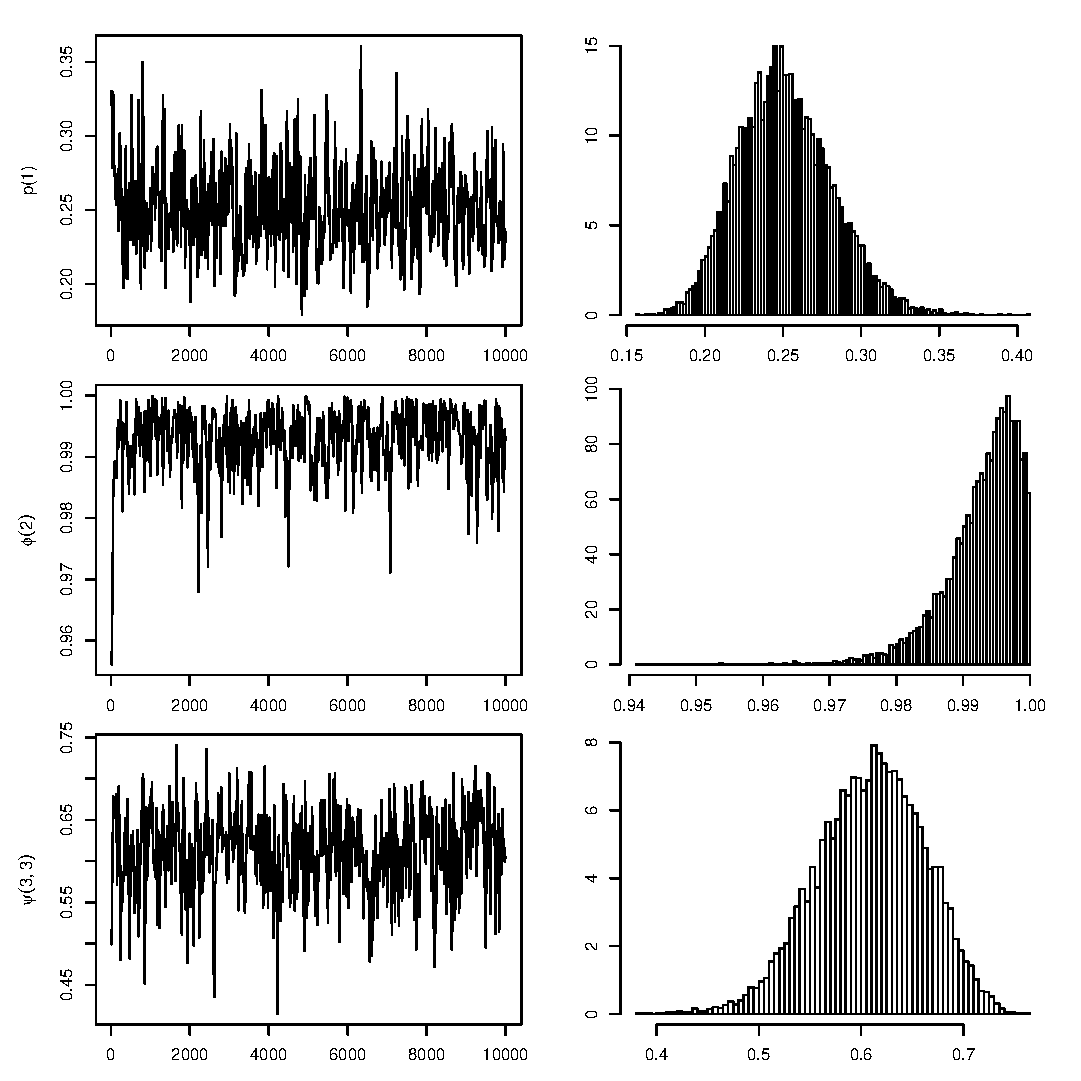
\includegraphics[width=\textwidth,height=6cm]{figures/g3.eps}}

\end{slide}

\section{Mixture models}
\begin{slide}\slidetitle{Mixture models}
\tableofcontents[sectionstyle=show/hide,subsectionstyle=show/shaded/hide]

\end{slide}
%%%%%%%%%%%%%%%%%%%%%%%%%%%%%%%%%%%%%%%
\begin{slide}\slidetitle{Missing variable models}

Complexity of a model may originate from the fact
that some piece of information is {\em missing}

\vs\pause
\begin{example}
Arnason--Schwarz model with missing zones\\
Probit model with missing normal variate
\end{example}

\vs\pause
Generic representation
$$
f(\bx|\theta) = \int_\mathscr{Z} g(\bx,\bz|\theta)\,\hbox{d}\bz
$$
\end{slide}
\subsection{Mixture models}\begin{slide}
\slidetitle{Mixture models}

Models of {\it mixtures of distributions}:
$$
x \sim f_{j} \hbox{ with probability }p_{j},
$$
for $j=1, 2, \ldots, k$, with overall density
\BrickRed{$$
p_{1} f_{1}(x) +\cdots+ p_{k} f_{k}(x) \; .
$$}
\pause
Usual case: parameterised components
$$
\sum_{i=1}^k p_i f(x|\theta_i)
$$
where {\em weights} $p_i$'s are distinguished from other parameters

\end{slide}\begin{slide}\slidetitle{Motivations}

\begin{itemize}
\item  Dataset made of several latent/missing/unobserved strata/subpopulations. 
Mixture structure due to the missing origin/allocation of each observation
to a specific subpopulation/stratum. Inference on either the allocations (clustering)
or on the parameters $(\theta_i,p_i)$ or on the number of groups
\vss\pause
\item  Semiparametric perspective where mixtures are basis
approximations of unknown distributions
\end{itemize}
\end{slide}\begin{slide}\slidetitle{{\sf License}}

Dataset derived from license plate image

Grey levels concentrated on $256$ values later jittered

\vs
\centerline{
\includegraphics[width=8cm]{figures/plate.eps}}
\centerline{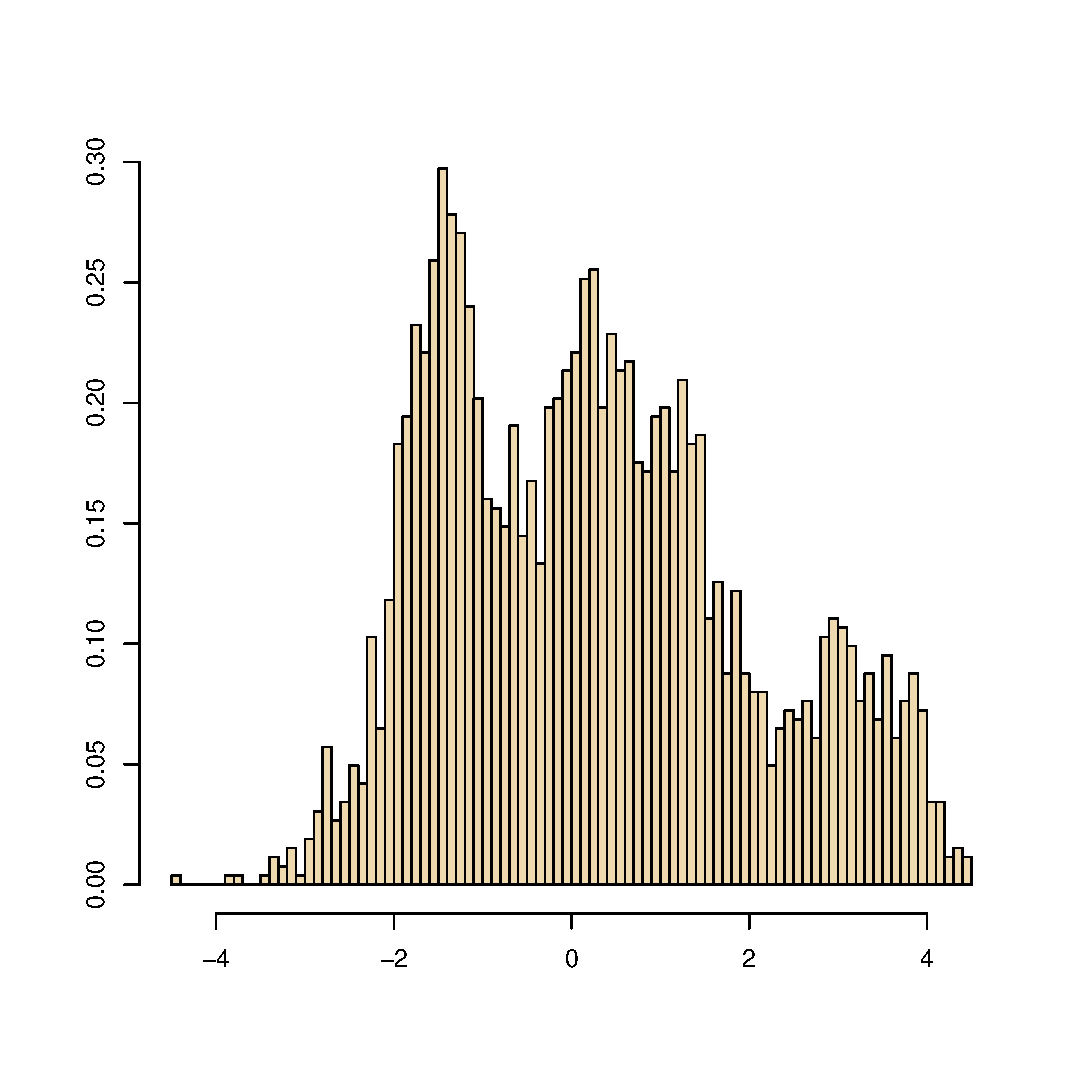
\includegraphics[height=4.5cm]{figures/plaque.hist.eps}}

\end{slide}\begin{slide}\slidetitle{Likelihood}

For a sample of independent random variables $(x_{1},\cdots,x_{n})$, likelihood
$$
\prod_{i=1}^n \left\{ p_{1} f_{1}(x_i) +\cdots+ p_{k} f_{k}(x_i) \right\} \;. 
$$

\vs\pause
Expanding this product involves 
$$
\RawSienna{k^{n}}
$$
elementary terms: prohibitive to compute in large samples.  

But likelihood still computable [pointwise] in $\text{O}(kn)$ time.
 
\end{slide}\begin{slide}\slidetitle{Normal mean benchmark}

Normal mixture
$$
p\,\mathscr{N}(\mu_1,1)+(1-p)\,\mathscr{N}(\mu_2,1)
$$
with only unknown means ($2$-D representation possible)

\begin{block}{Identifiability}
\begin{columns}\column{.45\textwidth}\small
Parameters $\mu_1$ and $\mu_2$ identifiable: $\mu_1$ cannot be confused with $\mu_2$ when
$p$ is different from $0.5$.

Presence of a spurious mode, understood by letting $p$ go to $0.5$\normalsize
\column{.5\textwidth}
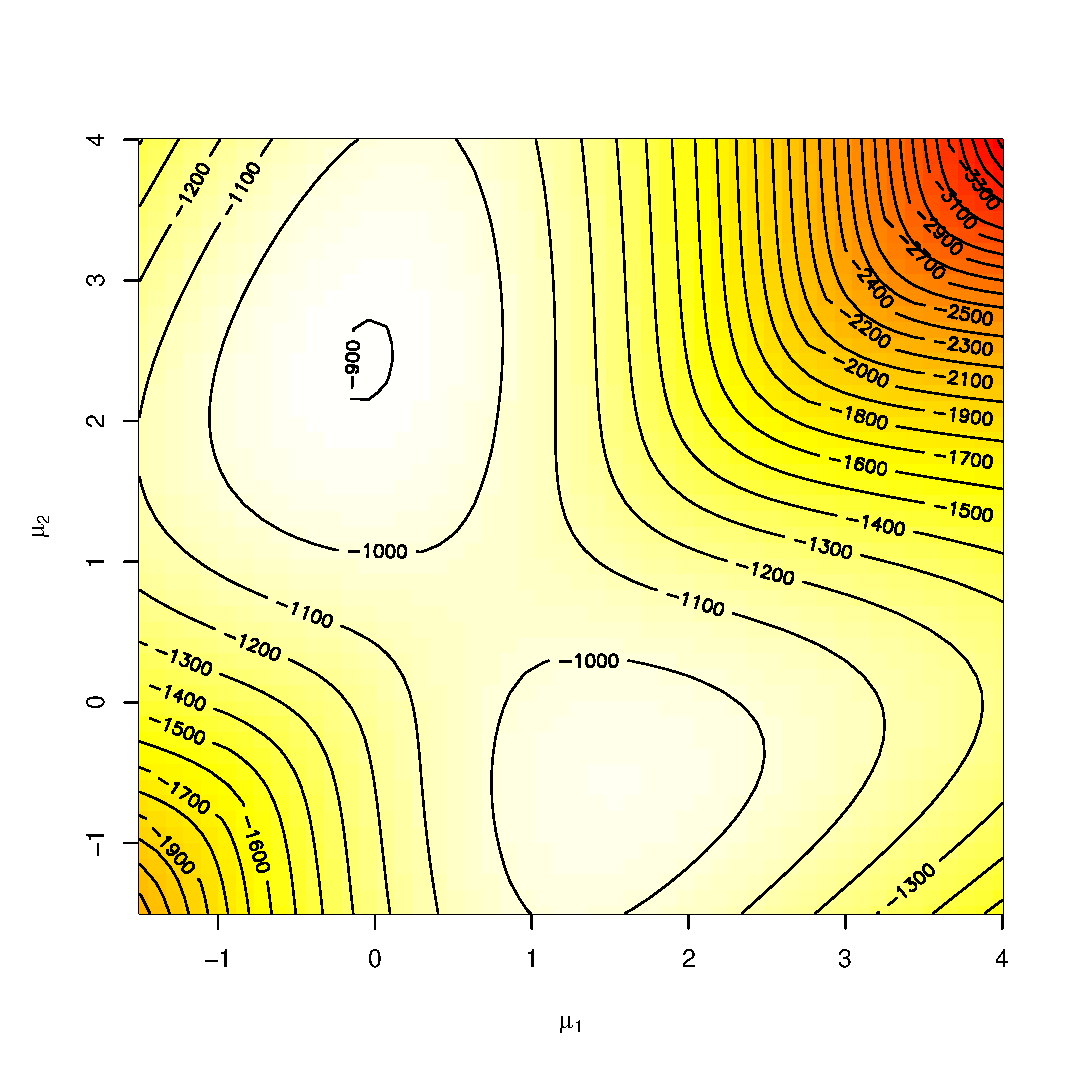
\includegraphics[width=.75\textwidth,height=.4\textheight]{figures/lvraisd1.eps}
\end{columns}
\end{block}

\end{slide}\begin{slide}
\slidetitle{Bayesian Inference}

For any prior $\pi\left(\btheta,\bp\right)$, posterior
distribution of $(\btheta,\bp)$ available up to a multiplicative constant
\small$$
\pi(\btheta,\bp|\bx) \propto \left[\prod_{i=1}^n \sum_{j=1}^k p_j\,f(x_i|\theta_j)\right] 
	\,\pi\left(\btheta,\bp\right)\,.
$$\normalsize
at a cost of order $\text{O}(kn)$

\vs\pause
\begin{block}{Difficulty}
Despite this, derivation of posterior characteristics like posterior expectations
only possible in an exponential time of order $\hbox{O}(k^n)$!
\end{block}

\end{slide}\begin{slide}
\slidetitle{Missing variable representation}

Associate to each $x_i$ a missing/latent variable $z_i$ that indicates its component:
$$
z_i|\bp\sim\mathscr{M}_k(p_1,\allowbreak\ldots,\allowbreak p_k)
$$
and
$$
x_i|z_i,\btheta \sim f(\cdot|\theta_{z_i})\,.
$$
\pause
Completed likelihood 
\small$$
\ell(\btheta,\bp|\bx,\bz)=\prod_{i=1}^n p_{z_i}\,f(x_i|\theta_{z_i})\,,
$$
and
$$
\pi(\btheta,\bp|\bx,\bz) \propto \left[\prod_{i=1}^n p_{z_i}\,f(x_i|\theta_{z_i})\right] 
\pi\left(\btheta,\bp\right)\,,
$$
\normalsize where $\bz=(z_1,\ldots,z_n)$.

\end{slide}\begin{slide}
\slidetitle{Partition sets}

Denote by $\mathcal{Z}=\{1,\ldots,k\}^n$
set of the $k^n$ possible vectors $\bz$.\\
$\mathcal{Z}$ decomposed into a partition of sets
$$
\displaystyle \mathcal{Z}=\cup_{j=1}^\mathfrak{r} \mathcal{Z}_j
$$
For a given allocation size vector
$\left(n_1,\ldots,n_k\right)$, where $n_1+\ldots+n_k=n$, 
{\em partition sets}
\small$$
\mathcal{Z}_j = \left\{\bz:\sum_{i=1}^n\mathbb{I}_{z_i=1}=n_1,
\ldots,\sum_{i=1}^n\mathbb{I}_{z_i=k}=n_k\right\}\,,
$$\normalsize
for all allocations with the given allocation size $\left(n_1,\ldots,n_k\right)$ 
and where labels $j=j(n_1,\ldots,n_k)$ defined by lexicographical ordering on the
$\left(n_1,\ldots,n_k\right)$'s.\\
%\pause\footnotesize[This means that $j=1$ corresponds to
%$\left(n_1,\ldots,n_k\right)=(n,0,\ldots,0)$, $j=2$ to
%$\left(n_1,\ldots,n_k\right)=(n-1,1,\ldots,0)$, $j=3$ to
%$\left(n_1,\ldots,n_k\right)=(n-1,0,1,\ldots,0)$, and so on.]\normalsize
%
\end{slide}\begin{slide}
\slidetitle{Posterior closed form representations}

$$
\pi\left(\btheta,\bp|\bx\right)=\sum_{i=1}^\mathfrak{r}\sum_{\bz \in\mathcal{Z}_i}
\omega\left(\bz\right) \pi\left(\btheta,\bp|\bx,\bz\right)\,,
$$
where $\omega\left(\bz\right)$ represents marginal posterior probability
of the allocation $\bz$ conditional on $\bx$
{\em [derived by integrating out the parameters $\btheta$ and $\bp$]}

\vs\pause
Bayes estimator of $\left(\btheta, \bp\right)$ 
$$
\sum_{i=1}^\mathfrak{r}\sum_{\bz\in\mathcal{Z}_i}\omega\left(\bz\right) 
\mathbb{E}^\pi\left[\btheta,\bp|\bx,\bz\right]\,.
$$

\vs\pause
\centerline{\RedOrange{\fbox{\bf \copyright\ \ Too costly: $2^n$ terms}}}

\end{slide}\subsection{MCMC approaches}
\begin{slide}
\slidetitle{General Gibbs sampling for mixture models}
Take advantage of the missing data structure:\\

\begin{block}{Algorithm}
{\sffamily
\begin{itemize}
\item  
	{\bfseries Initialization:} 
		 choose $\bp^{(0)}$ and $\btheta^{(0)}$ arbitrarily
\item  {\bfseries Step t.} For $t=1,\ldots$
\begin{enumerate}
\item Generate $z_i^{(t)}$ ($i=1,\ldots,n$) from ($j=1,\ldots,k$)
                 \begin{center}
                 $\mathbb{P}\left(z_i^{(t)}=j|p_j^{(t-1)},\theta_j^{(t-1)},x_i\right)\propto 
                 p_j^{(t-1)}f\left(x_i|\theta_j^{(t-1)}\right)$
                 \end{center}
\item Generate $\bp^{(t)}$ from $\pi(\bp|\bz^{(t)})$, 
\item Generate $\btheta^{(t)}$ from $\pi(\btheta|\bz^{(t)},\bx)$.
\end{enumerate}
\end{itemize}
}
\end{block}

\end{slide}\begin{slide}
\slidetitle{Exponential families}
When
$$
f(x|\theta)=h(x)\exp(R(\theta)\cdot T(x)>-\psi(\theta))
$$
simulation of both $\bp$ and $\btheta$
usually straightforward:\\

\RedOrange{{\bf Conjugate prior}} on $\theta_j$ given by\hyperlink{conju}{\beamerreturnbutton{Back 
to definition}}
$$
\pi_j(\theta)\propto \exp(R(\theta)\cdot \alpha_j-\beta_j\psi(\theta))\,,
$$
where $\alpha_j\in\mathbb{R}^k$ and $\beta_j>0$ are hyperparameters and
$$
\bp\sim\mathscr{D}\left(\gamma_1,\ldots,\gamma_k\right)
$$
{\em [Dirichlet distribution]}

\end{slide}\begin{slide}
\slidetitle{Gibbs sampling for exponential family mixtures}

\begin{block}{Algorithm}
{\sffamily
\begin{itemize}
\item  {\bfseries Initialization.} 
		 Choose $\bp^{(0)}$ and $\btheta^{(0)}$,
\item  {\bfseries Step t.} For $t=1,\ldots$
\begin{enumerate}
\item Generate $z_i^{(t)}$ ($i=1,\ldots,n,\,j=1,\ldots,k$) from 
         \small$$\mathbb{P}\left(z_i^{(t)}=j|p_j^{(t-1)},\theta_j^{(t-1)},x_i\right)
           \propto p_j^{(t-1)}f\left(x_i|\theta_j^{(t-1)}\right)$$ \normalsize
\item Compute $n_j^{(t)}=\sum_{i=1}^n\mathbb{I}_{z_i^{(t)}=j}$, 
		         $s_j^{(t)}=\sum_{i=1}^n\mathbb{I}_{z_i^{(t)}=j}t(x_i)$ 
\item Generate $\bp^{(t)}$ from 
	$\mathscr{D}\left(\gamma_1+n_1,\ldots,\gamma_k+n_k\right)$, 
\item Generate $\theta_j^{(t)}$ ($j=1,\dots,k$) from
  \small$$\pi(\theta_j|\bz^{(t)},\bx)\propto
  \exp\left(R(\theta_j)\cdot(\alpha+s_j^{(t)})-\psi(\theta_j)(n_j+\beta)\right).$$\normalsize
\end{enumerate}
\end{itemize}
}
\end{block}

\end{slide}\begin{slide}
\slidetitle{Normal mean example}

For mixture of two normal distributions with unknown means,
$$
p {\cal{N}}(\mu,\tau^{2}) + (1-p) {\cal{N}}(\theta,\sigma^{2}) \;,
$$
and a normal prior $\mathscr{N}\left(\delta,1/\lambda\right)$ on
$\mu_1$ and $\mu_2$, 

\end{slide}\begin{slide}
\slidetitle{Normal mean example (cont'd)}

\begin{block}{Algorithm}\small
{\sffamily
\begin{itemize}
\item  {\bfseries Initialization.} Choose $\mu_1^{(0)}$ and $\mu_2^{(0)}$,
\item  {\bfseries Step t.} For $t=1,\ldots$
\begin{enumerate}
\item Generate $z_i^{(t)}$ ($i=1,\ldots,n$) from 
                 $$\mathbb{P}\left(z_i^{(t)}=1\right)=1-\mathbb{P}\left(z_i^{(t)}=2\right)\propto
                 p\exp\left(-\frac{1}{2}\left(x_i-\mu_1^{(t-1)}\right)^2\right)$$
\item Compute $\displaystyle n_j^{(t)}=\sum_{i=1}^n\mathbb{I}_{z_i^{(t)}=j}$ and 
                 $\displaystyle (s^x_j)^{(t)}=\sum_{i=1}^n\mathbb{I}_{z_i^{(t)}=j}x_i$
\item Generate $\mu_j^{(t)}$ ($j=1,2$) from $\displaystyle 
	\mathscr{N}\left(\frac{\lambda\delta+(s^x_j)^{(t)}}{\lambda+n_j^{(t)}},
       		\frac{1}{\lambda+n_j^{(t)}}\right)$.
\end{enumerate}
\end{itemize}
}
\end{block}\normalsize

\end{slide}\begin{slide}
\slidetitle{Normal mean example (cont'd)}

\begin{columns}\column{.5\textwidth}
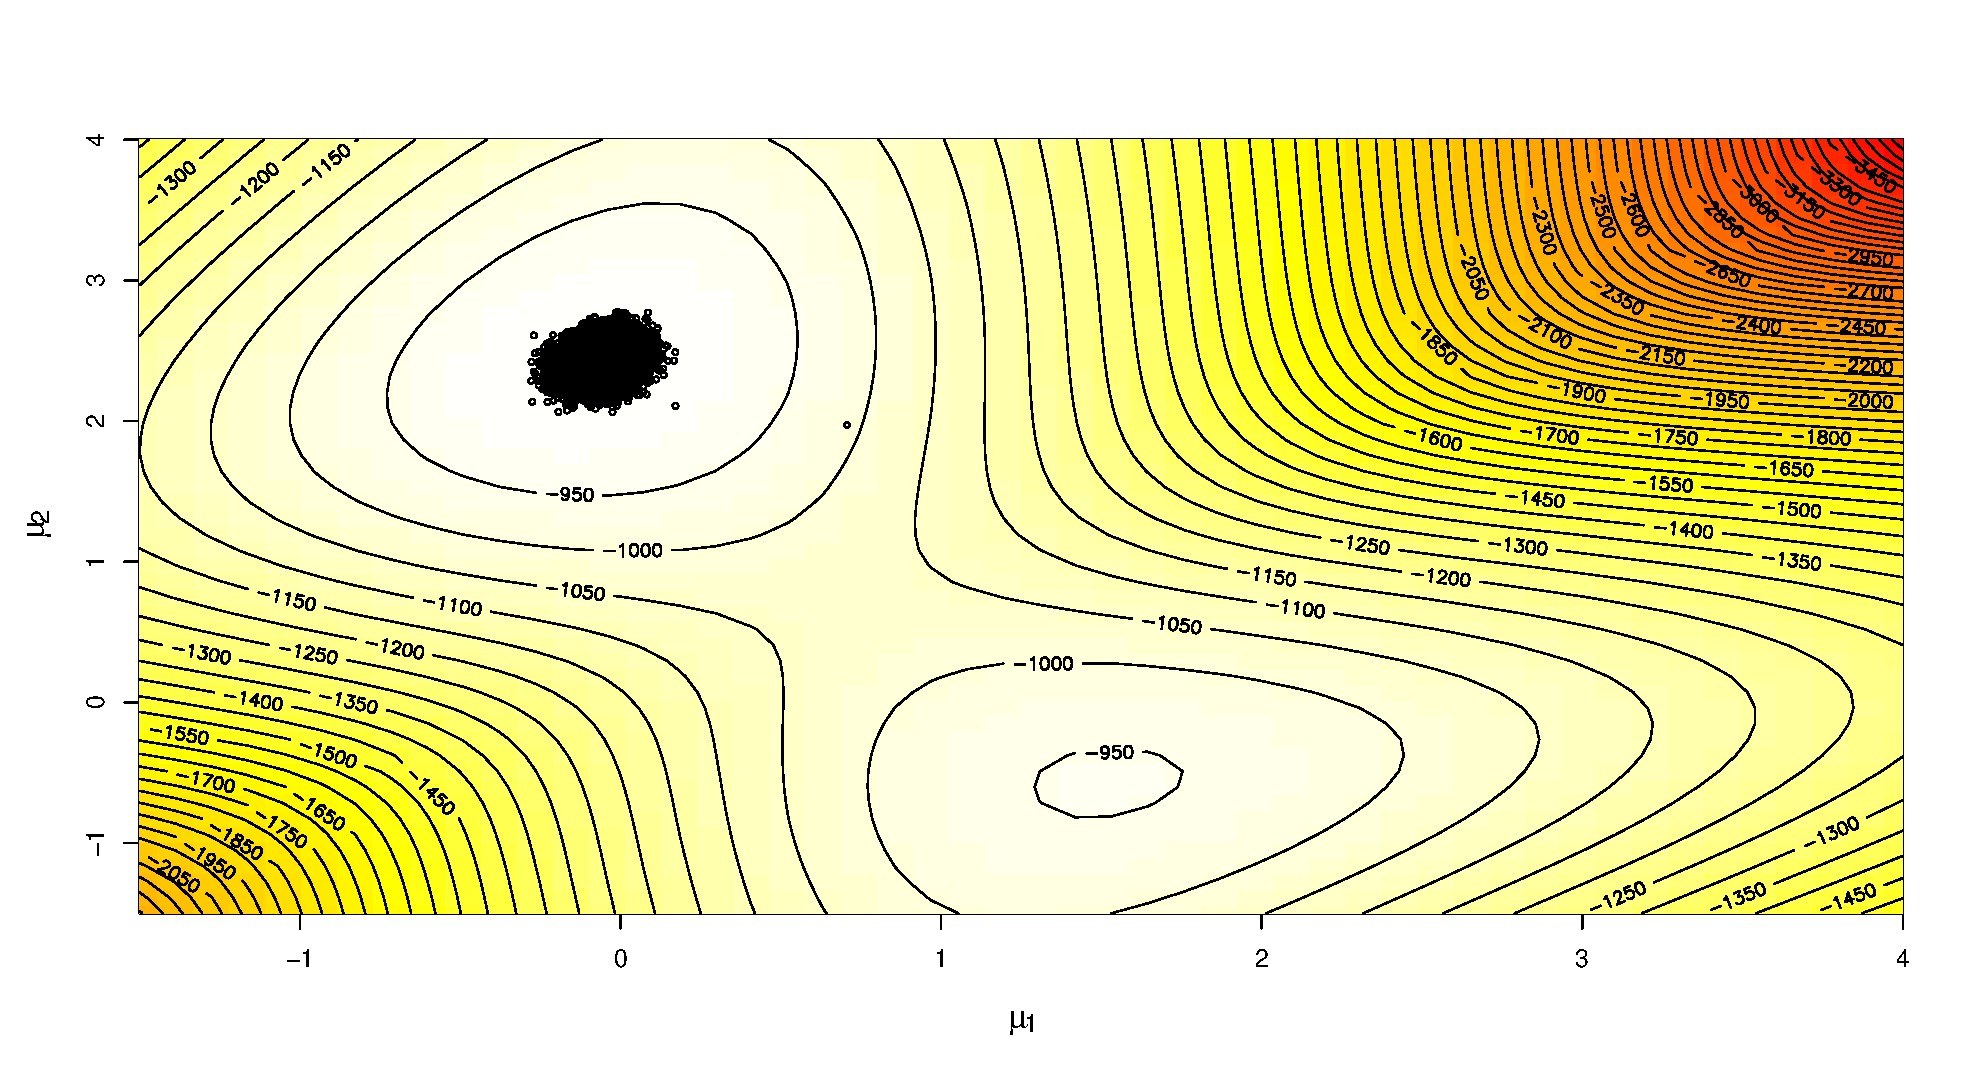
\includegraphics[width=\textwidth,height=6cm]{figures/g2n2d1.eps}\\
{\bf (a) initialised at random}
\column{.5\textwidth}
\only<2>{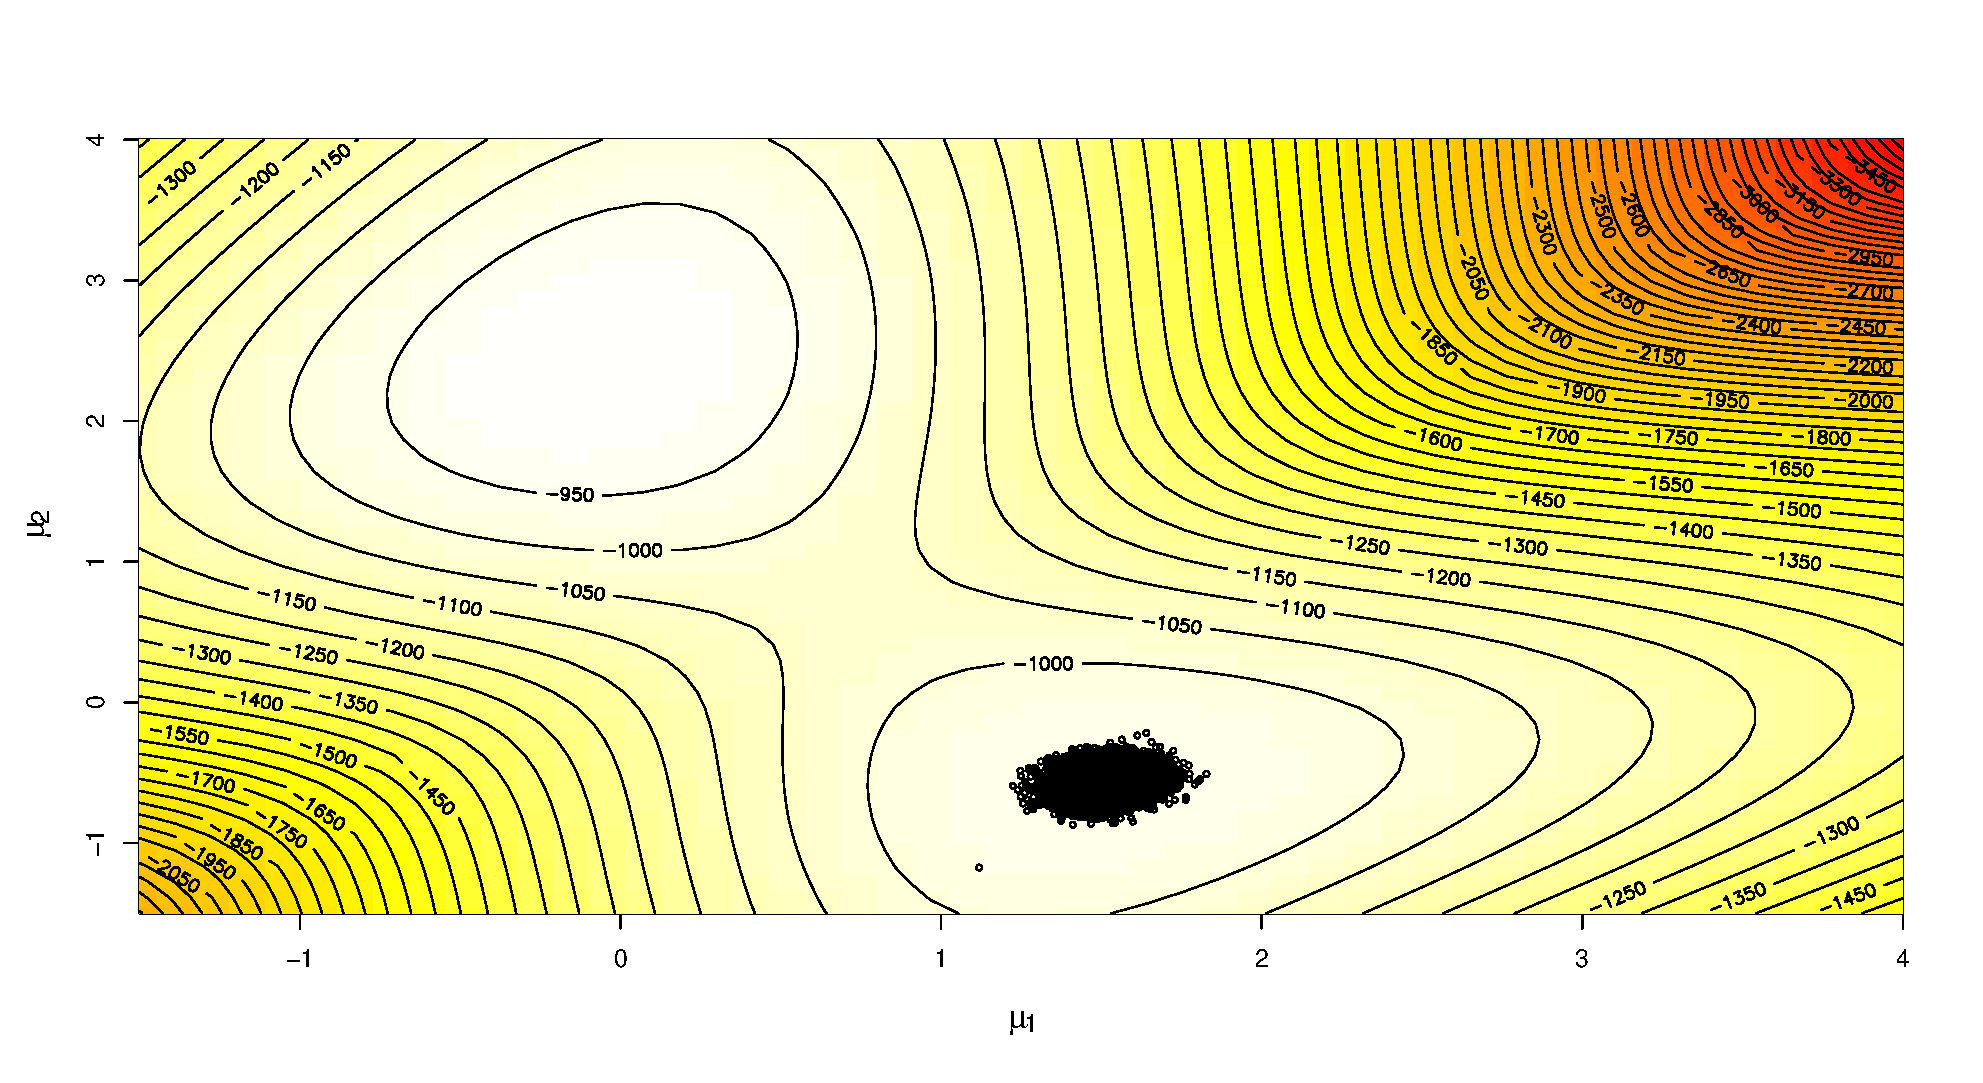
\includegraphics[width=\textwidth,height=6cm]{figures/g1n2d1.eps}\\
{\bf (b) initialised close to the lower mode}}
\end{columns}

\end{slide}\begin{slide}
\slidetitle{{\sf License}}

Consider $k=3$ components, a $\mathscr{D}_3(1/2,1/2,1/2)$ prior for the weights,
a $\mathscr{N}(\overline{x},\hat\sigma^2/3)$
prior on the means $\mu_i$ and a
$\mathscr{G}a(10,\hat\sigma^2)$ prior on the precisions
$\sigma_i^{-2}$, where $\overline{x}$ and $\hat\sigma^2$ are the
empirical mean and variance of {\sf License}
\emfarite{Empirical Bayes}

\pause
\centerline{\includegraphics[width=.8\textwidth,height=4cm]{figures/mixt.est.eps}}

\end{slide}\begin{slide}
\slidetitle{Metropolis--Hastings alternative}

For the Gibbs sampler, completion of $\bz$ increases the dimension of the simulation space 
and reduces the mobility of the parameter chain.

\vs\pause
Metropolis--Hastings algorithm available since posterior 
available in closed form, as long as $q$ provides a correct
exploration of the posterior surface, since 
$$
\frac{\pi(\btheta^\prime,\bp^\prime|\bx)}{\pi(\btheta,\bp|\bx)}\,
\frac{q(\btheta,\bp|\btheta^\prime,\bp^\prime)}{q(\btheta^\prime,\bp^\prime|\btheta,\bp)}\wedge 1
$$
computable in \BrickRed{{\bf O$(kn)$}} time

\end{slide}\begin{slide}
\slidetitle{Random walk Metropolis--Hastings}

Proposal distribution for the new value
$$
\widetilde{\theta_j}=\theta_j^{(t-1)}+u_j\hbox{ where }u_j\sim\mathscr{N}(0,\zeta^2)
$$

\vs\pause
\begin{columns}\column{.6\textwidth}
In mean mixture case, Gaussian random walk proposal is
\begin{align*}
\widetilde{\mu_1}&\sim\mathscr{N}\left(\mu_1^{(t-1)},\zeta^2\right)\quad\hbox{and}\\
\widetilde{\mu_2}&\sim\mathscr{N}\left(\mu_2^{(t-1)},\zeta^2\right)\,
\end{align*}
\column{.4\textwidth}
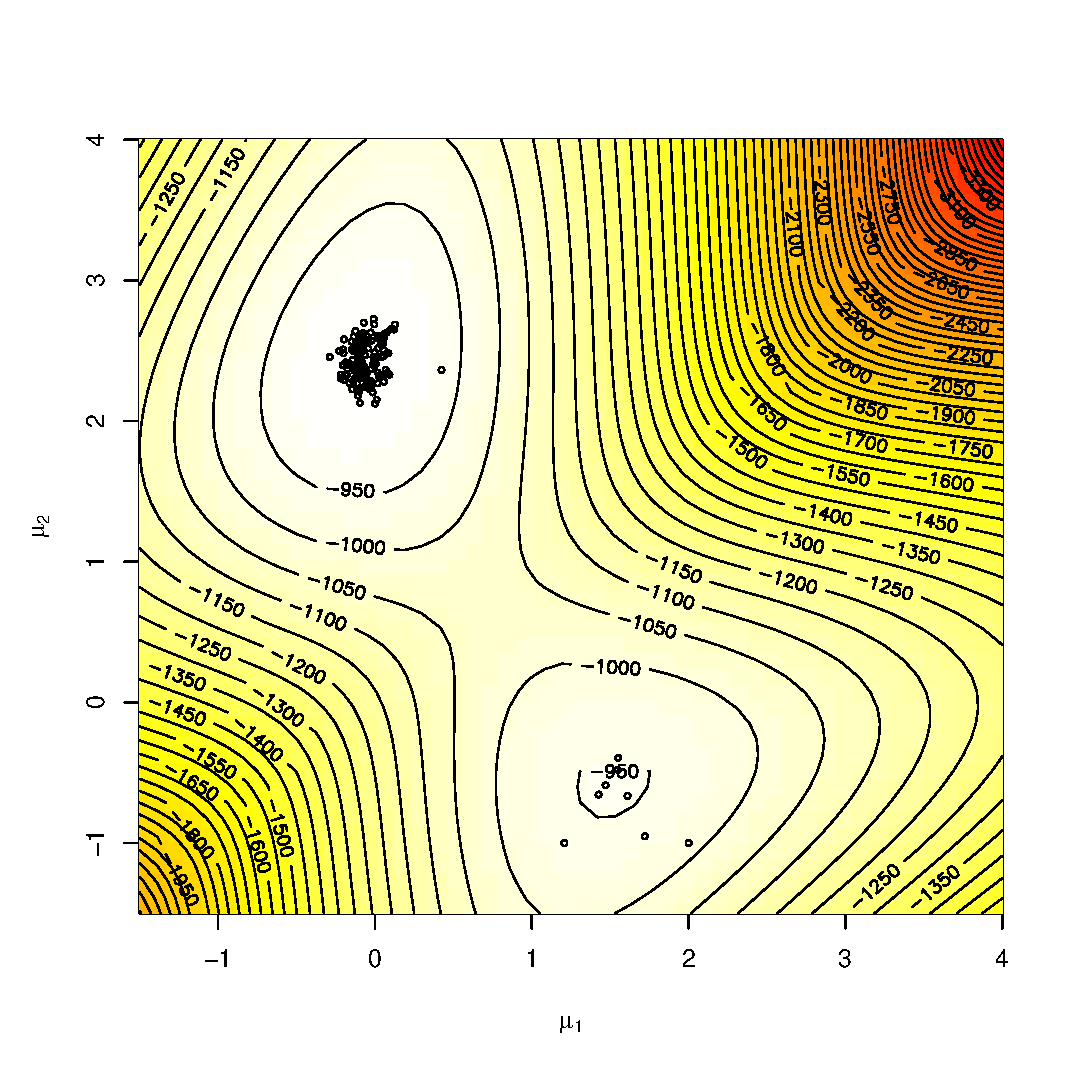
\includegraphics[height=4cm,width=4cm]{figures/hmn2d1.eps}
\end{columns}

\end{slide}\begin{slide}
\slidetitle{Random walk Metropolis--Hastings for means}

\begin{block}{Algorithm}
{\sf
\begin{itemize}
\item {\sffamily Initialization:}\\
    Choose $\mu_1^{(0)}$ and $\mu_2^{(0)}$
\item  {\sffamily Iteration $t$ $(t\ge 1)$:}
\begin{enumerate}
\item Generate $\widetilde{\mu_1}$ from $\mathscr{N}\left(\mu_1^{(t-1)},\zeta^2\right)$,
\item Generate $\widetilde{\mu_2}$ from $\mathscr{N}\left(\mu_2^{(t-1)},\zeta^2\right)$,
\item Compute
$$
r={\pi\left(\widetilde{\mu_1},\widetilde{\mu_2}|x\right)}\big/{\pi\left(\mu_1^{(t-1)},\mu_2^{(t-1)}|x\right)}
$$
\item Generate $u\sim\mathscr{U}_{[0,1]}$: if $u<r$, then 
$\left(\mu_1^{(t)}, \mu_2^{(t)}\right)=\left(\widetilde{\mu_1},\widetilde{\mu_2}\right)$ \\
                 else $\left(\mu_1^{(t)},\mu_2^{(t)}\right)=\left(\mu_1^{(t-1)},\mu_2^{(t-1)}\right)$.
\end{enumerate}
\end{itemize}
}
\end{block}

\end{slide}\begin{slide}
\slidetitle{Random walk extensions}

Difficulties with \MidnightBlue{{\bf constrained parameters}}, 
like $\bp$ such that \centerline{$\sum_{i=1}^kp_k\allowbreak=1$.}\\

\vs Resolution by overparameterisation
\small$$p_j={w_j}\bigg/{\displaystyle \sum_{l=1}^kw_l}\,,\quad w_j>0\,,$$\normalsize
and proposed move on the 
$w_j$'s 
\small$$\log(\widetilde{w_j})=\log(w_j^{(t-1)})+u_j\hbox{ where }u_j\sim\mathscr{N}(0,\zeta^2)$$
\normalsize
\vs\pause
\begin{itemize}
\item[$\lightning$] Watch out for the Jacobian in the $\log$ transform
\end{itemize}

\end{slide}\subsection{Label switching}\begin{slide}
\slidetitle{Identifiability}

A mixture model is invariant under
permutations of the indices of the components.\\

E.g., mixtures 
$$
0.3\mathscr{N}(0,1)+0.7\mathscr{N}(2.3,1)
$$
and
$$
0.7\mathscr{N}(2.3,1)+0.3\mathscr{N}(0,1)
$$
are \BurntOrange{{\bf exactly}} the same!

\vs\pause
\MidnightBlue{{\bf \copyright~ The component parameters $\theta_i$ are not identifiable {\em marginally} since
they are exchangeable}}

\end{slide}\begin{slide}
\slidetitle{Connected difficulties}

\begin{enumerate}
\item Number of modes of the likelihood of order $\mathrm{O}(k!)$:\\
\copyright~Maximization and even [MCMC] exploration of the posterior surface harder 

\pause
\item Under exchangeable priors on $(\btheta,\bp)$
{\em [prior invariant under permutation of the indices]}, all 
posterior marginals are identical:\\
\copyright~Posterior expectation of $\theta_1$ equal to posterior expectation of $\theta_2$.
\end{enumerate}

\end{slide}\begin{slide}
\slidetitle{{\sf License}}

Since Gibbs output does not produce exchangeability, the Gibbs sampler has not explored the
whole parameter space: it lacks energy to switch simultaneously enough component allocations 
at once

\centerline{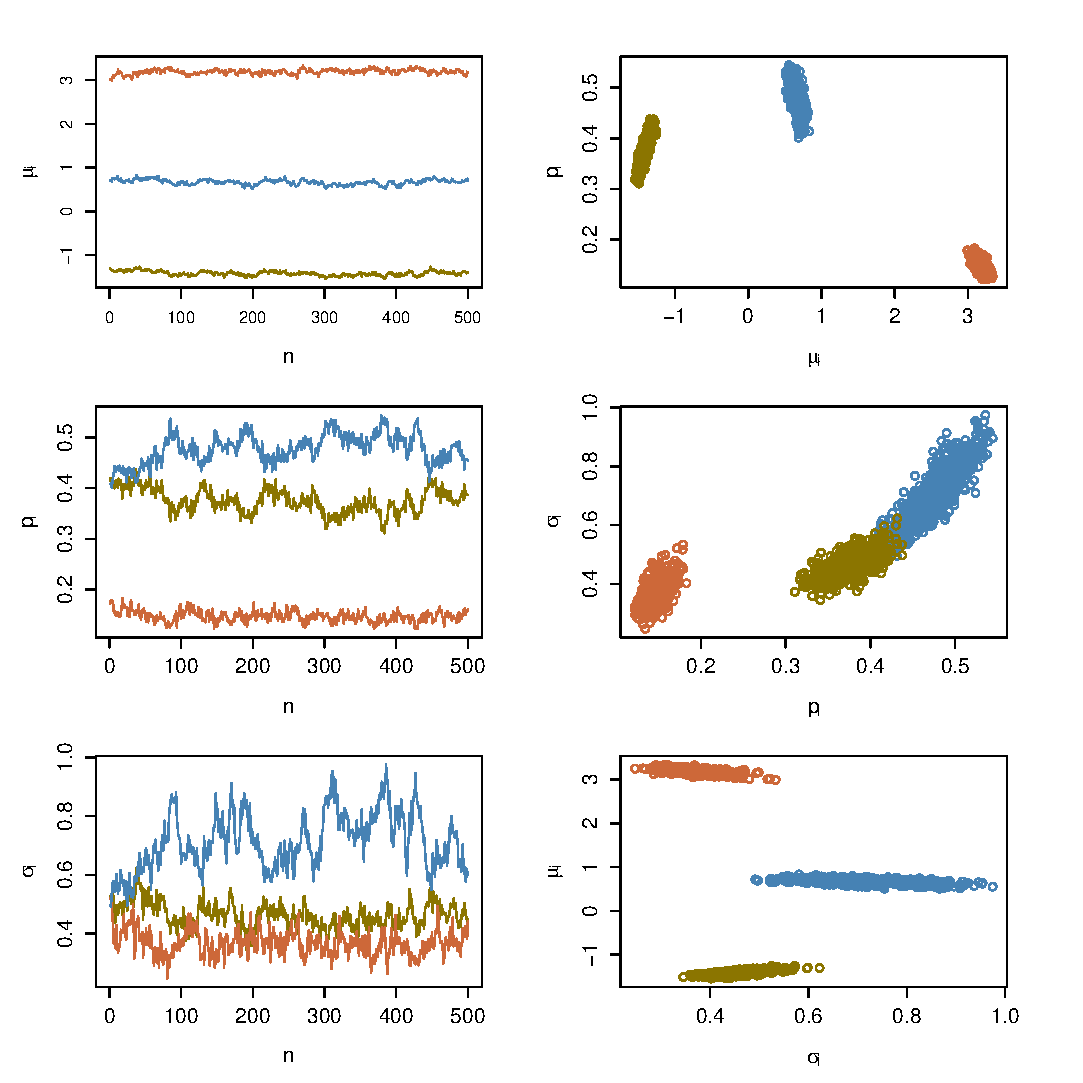
\includegraphics[height=5cm,width=10cm]{figures/mixt.noX.eps}}

\end{slide}\begin{slide}
\slidetitle{Label switching paradox}

We should observe the exchangeability of the components [label switching] to conclude
about convergence of the Gibbs sampler. 

\vs\pause If we observe it, then we do not know how to
estimate the parameters. 

\vs\pause If we do not, then we are uncertain about the convergence!!!

\end{slide}\begin{slide}
\slidetitle{Constraints}

Usual reply to lack of identifiability: impose constraints like ${\mu_1\le\ldots\le\mu_k}$
in the prior

\vs\pause Mostly incompatible with the topology of the posterior surface: posterior 
expectations then depend on the choice of the constraints.

\vs\pause
\begin{block}{Computational detail}
The constraint does not need to be imposed {\em during} the simulation
but can instead be imposed {\em after} simulation, by reordering the
MCMC output according to the constraint. This avoids possible negative effects
on convergence.
\end{block}

\end{slide}\begin{slide}
\slidetitle{Relabeling towards the mode}

Selection of one of the $k!$ modal regions of the posterior once simulation is over,
by computing the approximate MAP
\small$$
(\btheta,\bp)^{(i^*)}\quad\text{with}\quad
i^*=\arg\max_{i=1,\ldots,M} \pi\left\{ (\btheta,\bp)^{(i)}|\bx \right\}
$$\normalsize

\pause
\begin{block}{Pivotal Reordering}
At iteration $i\in\{1,\ldots,M\}$,
\begin{enumerate}
\item Compute the optimal permutation
\small$$
\tau_i=\arg\min_{\tau\in\mathfrak{S}_k} d\left(\tau\left\{
(\btheta^{(i)},\bp^{(i)}),(\btheta^{(i^*)},\bp^{(i^*)})
\right\}\right)
$$\normalsize
where $d(\cdot,\cdot)$ distance in the parameter space.
\item Set $(\btheta^{(i)},\bp^{(i)})=\tau_i((\btheta^{(i)},\bp^{(i)}))$.
\end{enumerate}
\end{block}

\end{slide}\begin{slide}
\slidetitle{Re-ban on improper priors}

Difficult to use improper priors in the setting of mixtures because independent improper priors,
$$
\pi\left(\btheta\right)=\prod_{i=1}^k\pi_i(\theta_i)\,,
\quad\text{with}\quad
\int\pi_i(\theta_i)\hbox{d}\theta_i=\infty
$$
end up, for all $n$'s, with the property
$$\int\pi(\btheta,\bp|\bx)
\hbox{d}\btheta\hbox{d}\bp=\infty\,.
$$ 

\pause
\begin{block}{Reason}
There are $(k-1)^n$ terms among the $k^n$ terms in the expansion that allocate {\em no
observation at all} to the  $i$-th component.
\end{block}

\end{slide}\begin{slide}
\slidetitle{Tempering}

Facilitate exploration of $\pi$ by flattening the target: simulate from $\pi_\alpha(x)\propto 
\pi(x)^\alpha$ for $\alpha>0$ large enough 

\vs\pause\begin{itemize}
\item Determine where the modal regions of $\pi$ are (possibly with parallel versions using
different $\alpha$'s)
\item Recycle simulations from $\pi(x)^\alpha$ into simulations from $\pi$ by importance sampling
\item Simple modification of the Metropolis--Hastings algorithm, with new acceptance
$$
\left\{ \left(\frac{\pi(\btheta^\prime,\bp^\prime|\bx)} {\pi(\btheta,\bp|\bx)}\right)^\alpha\,
\frac{q(\btheta,\bp|\btheta^\prime,\bp^\prime)} {q(\btheta^\prime,\bp^\prime|\btheta,\bp)}\right\} \wedge 1
$$
\end{itemize}

\end{slide}\begin{slide}
\slidetitle{Tempering with the mean mixture}

\includegraphics[width=11cm,height=5cm]{figures/tempix.eps}
%\includegraphics[width=4cm,height=5cm]{figures/tempix1.eps}
%\only{2-3}{\includegraphics[width=4cm,height=5cm]{figures/tempix2.eps}}
%\only<3>{\includegraphics[width=4cm,height=5cm]{figures/tempix3.eps}}

\end{slide}\subsection{MCMC for variable dimension models}\begin{slide}
\slidetitle{MCMC for variable dimension models}

\begin{columns}\column{.5\textwidth}
\small\begin{flushleft}
\begin{quote}
One of the things we do not know is\\
the number of things we do not know\\
---P.~Green, 1996---
\end{quote}
\end{flushleft}\normalsize
\column{.5\textwidth}
\begin{flushright}\includegraphics[width=3cm]{figures/peterG.eps}\end{flushright}
\end{columns}

\pause
\begin{example} \begin{itemize}
\item the number of components in a mixture
\item the number of covariates in a regression model
\item the number of different capture probabilities in a capture-recapture model
\item the number of lags in a time-series model
\end{itemize} \end{example}

\end{slide}\begin{slide}
\slidetitle{Variable dimension models}

Variable dimension model defined as a collection of models $(k=1.\ldots,K)$,
$$
   \GoM_k = \left\{ f(\cdot|\theta_k);\ \theta_k\in\Theta_k \right\}\,,
$$
associated with a collection of priors on the parameters of these models,
$$
  \pi_k(\theta_k)\,,
$$
and a prior distribution on the indices of these models,
$$
\left\{ \varrho(k)\,,k=1,\ldots,K \right\} \,.
$$

Global notation:
$$\RawSienna{
  \pi(\GoM_k,\theta_k) = \varrho(k)\,\pi_k(\theta_k)
}$$

\end{slide}\begin{slide}
\slidetitle{Bayesian inference for variable dimension models}

Two perspectives:
\begin{enumerate}
\item consider the variable dimension model as a {\em whole} and estimate quantities meaningful 
for the whole like predictives
\small$$
%f(x|x_1,\ldots,x_n) &= \\ &
\sum_k \hbox{Pr}({\mathfrak M}_k|x_1,\ldots,x_n)
\int \,f_k(x|\theta_k) \hbox{d}x\,\pi_k(\theta_k|x_1,\ldots,x_n) \hbox{d}\theta\,.
$$\pause\normalsize
\&\ quantities only meaningful for submodels (like moments of $\theta_k$), computed
from $\pi_k(\theta_k|x_1,\ldots,x_n)$. {\em [Usual setup]}

\item resort to testing by choosing the best submodel via
\footnotesize$$
p(\GoM_i|x) = { \displaystyle{p_i \int_{\Theta_i} f_i(x|\theta_i) 
         \pi_i(\theta_i) d\theta_i} \over
\displaystyle{\sum_j p_j \int_{\Theta_j} f_j(x|\theta_j) \pi_j(\theta_j) 
      d\theta_j}  }  
$$\normalsize
\end{enumerate}

\end{slide}\begin{slide}
\slidetitle{Green's reversible jumps}

Computational burden in exploring [possibly infinite] complex parameter space:
Green's method set up a proper measure--theoretic framework for
designing moves {\em between} models/spaces $\GoM_k$/$\Theta_k$
of varying dimensions {\em [no one-to-one correspondence]}

\vs\pause
Create a \Orange{{\bf reversible kernel}}
$\GoK$ on $\mathfrak{H}=\bigcup_k \{k\}\times\Theta_k$ such that 
$$
\int_A \int_B \GoK(x,dy) \pi(x) dx = \int_B \int_A \GoK(y,dx) \pi(y) dy
$$
for the invariant density $\pi$ [$x$ is of the form $(k,\theta^{(k)})$] 
and for all sets $A,B$ {\em [un-detailed balance]}

\end{slide}\begin{slide}
\slidetitle{Green's reversible kernel}

Since Markov kernel $\GoK$ necessarily of the form 
{\em [either stay at the same value or move to one of the states]}
$$
\GoK(x,B) = \sum_{m=1}^\infty \int \rho_m(x,y) \mathfrak{q}_m(x,dy) + \omega(x)\mathbb{I}_B(x)
$$
where $\mathfrak{q}_m(x,dy)$ transition measure to model $\GoM_m$ and $\rho_m(x,y)$
corresponding acceptance probability, \pause only need to consider proposals between two models,
$\GoM_1$ and $\GoM_2$, say.

\end{slide}\begin{slide}
\slidetitle{Green's reversibility constraint}

If transition kernels between those models are $\GoK_{1\rightarrow2}(\theta_1,d\theta)$ and
$\GoK_{2\rightarrow1}(\theta_2,d\theta)$, formal use of the \MidnightBlue{{\em detailed balance condition}
$$
\pi(d\theta_1)\, \GoK_{1\rightarrow 2}(\theta_1,d\theta) =
\pi(d\theta_2)\, \GoK_{2\rightarrow 1}(\theta_2,d\theta)\,,
$$}

\vs\pause
\begin{itemize}
\item[$\lightning$] To preserve stationarity, necessary symmetry between 
moves/proposals from $\GoM_1$ to $\GoM_2$ and from $\GoM_2$ to  $\GoM_1$
\end{itemize}


\end{slide}\begin{slide}
\slidetitle{Two-model transitions}

How to move from model $\GoM_1$ to $\GoM_2$,
with Markov chain being in state $\theta_1\in\GoM_1$ {\em [i.e. $k=1$]}?

\vs\pause
Most often $\GoM_1$ and $\GoM_2$ are of different dimensions, e.g.
\centerline{$\dim(\GoM_2)>\dim(\GoM_1)$.}

\vs In that case, need to supplement both spaces $\Theta_{k_1}$ and
$\Theta_{k_2}$ with adequate artificial spaces to create a
{\em one-to-one} mapping between them, most often by augmenting the space of
the smaller model. 

\end{slide}\begin{slide}
\slidetitle{Two-model completions}

E.g., move from  $\theta_2\in{\Theta}_2$ to ${\Theta}_1$ chosen to be
a {\em deterministic} transform of $\theta_2$
$$
\theta_1=\Psi_{2\rightarrow 1}(\theta_{2})\,,
$$

\pause
Reverse proposal expressed as
$$
\theta_2 = \Psi_{1\rightarrow 2}(\theta_1,v_{1\rightarrow 2})
$$
where $v_{1\rightarrow 2}$ r.v.~of dimension
$\dim(\GoM_2)-\dim(\GoM_1)$, generated as
$$
v_{1\rightarrow 2} \sim \varphi_{1\rightarrow 2}(v_{1\rightarrow 2})\,.
$$

\end{slide}\begin{slide}
\slidetitle{Two-model acceptance probability}

In this case, $\theta_2$ has density {\em [under stationarity]}
$$
\mathfrak{q}_{1\rightarrow 2}(\theta_2) =
\pi_1(\theta_1)\,\varphi_{1\rightarrow 2}(v_{1\rightarrow 2})\,
\left| \frac{\partial \Psi_{1\rightarrow 2}(\theta_1,v_{1\rightarrow 2})}{
             \partial (\theta_1,v_{1\rightarrow 2}) } \right|^{-1}\,,
$$
by the Jacobian rule. 

\pause
To make it $\pi_2(\theta_2)$ we thus need to accept this value with probability
$$
\alpha(\theta_1,v_{1\rightarrow 2}) = 1 \wedge \frac{\pi(\GoM_2,\theta_2)}
{\pi(\GoM_1,\theta_1)\, \varphi_{1\rightarrow 2}(v_{1\rightarrow 2})}\,
\left| \frac{\partial \Psi_{1\rightarrow 2}(\theta_1,v_{1\rightarrow 2})}{
\partial (\theta_1,v_{1\rightarrow 2}) } \right|\,.
$$

\begin{itemize}
\item[$\lightning$] This is restricted to the case when only moves between $\GoM_1$ and $\GoM_2$
		    are considered
\end{itemize}

\end{slide}\begin{slide}
\slidetitle{Interpretation}
The representation puts us back in a fixed dimension setting: 

\def\GoV{\mathfrak{V}}
\begin{itemize}
\item $\GoM_1\times\GoV_{1\rightarrow 2}$ and $\GoM_2$ in one-to-one relation.
\pause
\item reversibility imposes that $\theta_1$ is derived as
$$
(\theta_1,v_{1\rightarrow 2}) = \Psi_{1\rightarrow 2}^{-1}(\theta_2)
$$
\item appears like a {\em regular} Metropolis--Hastings move from the
couple $(\theta_1,v_{1\rightarrow 2})$ to $\theta_2$ 
when stationary distributions are
$\pi(\GoM_1,\theta_1)\times\varphi_{1\rightarrow 2}(v_{1\rightarrow 2})$
and $\pi(\GoM_2,\theta_2)$, and when proposal distribution is
{\em deterministic} (??) 
\end{itemize}

\end{slide}\begin{slide}
\slidetitle{Pseudo-deterministic reasoning}

Consider the proposals
$$
\theta_2\sim{\mathcal N}(\Psi_{1\rightarrow 2}
(\theta_1,v_{1\rightarrow 2}),\varepsilon)
\qquad\hbox{and}\qquad
\Psi_{1\rightarrow 2}(\theta_1,v_{1\rightarrow 2})\sim{\mathcal N}(\theta_2,\varepsilon)
$$

\pause Reciprocal proposal has density
\small$$
\frac{\exp\left\{-(\theta_2-\Psi_{1\rightarrow 2}
(\theta_1,v_{1\rightarrow 2}))^2/2\varepsilon\right\}}{\sqrt{2\pi\varepsilon}}
\times \left| \frac{\partial \Psi_{1\rightarrow 2}(\theta_1,v_{1\rightarrow 2})}{
     \partial (\theta_1,v_{1\rightarrow 2}) }\right|
$$\normalsize
by the Jacobian rule. 

Thus Metropolis--Hastings acceptance probability is
\small$$
1 \wedge \frac{\pi(\GoM_2,\theta_2)}{\pi(\GoM_1,\theta_1)\,
\varphi_{1\rightarrow 2}(v_{1\rightarrow 2})}\,
\left| \frac{\partial \Psi_{1\rightarrow 2}(\theta_1,v_{1\rightarrow 2})}{
\partial (\theta_1,v_{1\rightarrow 2}) }\right|
$$\normalsize

Does not depend on $\varepsilon$: \Maroon{{\bf Let $\varepsilon$ go to $0$}}

\end{slide}\begin{slide}
\slidetitle{Generic reversible jump acceptance probability}

If several models are considered simultaneously, with 
probability $\varpi_{1\rightarrow 2}$ of choosing move to $\GoM_2$ while in $\GoM_1$, 
as in 
\footnotesize$$
\GoK(x,B) = \sum_{m=1}^\infty \int \rho_m(x,y) \mathfrak{q}_m(x,dy) + \omega(x)\mathbb{I}_B(x)
$$\normalsize
\pause
acceptance probability of $\theta_2=\Psi_{1\rightarrow 2}(\theta_1,v_{1\rightarrow 2})$ is
\small$$\Red{
\alpha(\theta_1,v_{1\rightarrow 2}) =
1 \wedge \frac{\pi(\GoM_2,\theta_2)\,\varpi_{2\rightarrow 1}}
{\pi(\GoM_1,\theta_1)\,\varpi_{1\rightarrow 2}\,
\varphi_{1\rightarrow 2}(v_{1\rightarrow 2})}\,
\left| \frac{\partial \Psi_{1\rightarrow 2}(\theta_1,v_{1\rightarrow 2})}{
\partial (\theta_1,v_{1\rightarrow 2}) } \right|
}$$\normalsize
\pause while acceptance probability of $\theta_1$ with 
$(\theta_1,v_{1\rightarrow 2})=\Psi_{1\rightarrow 2}^{-1}(\theta_2)$ is
\small$$
\Red{
\alpha(\theta_1,v_{1\rightarrow 2}) =
1 \wedge \frac{\pi(\GoM_1,\theta_1)\,\varpi_{1\rightarrow 2}\,
\varphi_{1\rightarrow 2}(v_{1\rightarrow 2})}{\pi(\GoM_2,\theta_2)\,\varpi_{2\rightarrow 1}}\,
\left| \frac{\partial \Psi_{1\rightarrow 2}(\theta_1,v_{1\rightarrow 2})}{
\partial (\theta_1,v_{1\rightarrow 2}) } \right|^{-1}
}$$
\normalsize

\end{slide}\begin{slide}
\slidetitle{Green's sampler}

\begin{block}{Algorithm}
{\sffamily {\bfseries Iteration $t$ $(t\ge 1)$:} if $x^{(t)}=(m,\theta^{(m)})$,
\begin{enumerate}
\item Select model ${\mathfrak M}_n$ with probability $\pi_{mn}$
\item Generate $u_{mn}\sim\varphi_{mn}(u)$ and
                set $(\theta^{(n)},v_{nm})=\Psi_{m\rightarrow n}(\theta^{(m)},u_{mn})$
\item Take $x^{(t+1)} =( n,\theta^{(n)})$ with probability
\small$$
\min\left(
{\pi(n,\theta^{(n)}) \over \pi(m,\theta^{(m)})}
\;
{\pi_{nm} \varphi_{nm}(v_{nm}) \over \pi_{mn} \varphi_{mn}(u_{mn})}
\; \left| {\partial \Psi_{m\rightarrow n}(\theta^{(m)},u_{mn}) \over \partial
(\theta^{(m)},u_{mn})} \right|, 1 \right)
\normalsize$$
and take $x^{(t+1)} =x^{(t)}$ otherwise.
\end{enumerate}}\end{block}

\end{slide}\begin{slide}
\slidetitle{Mixture of normal distributions}
$$
\GoM_k =\left\{ (p_{jk},\mu_{jk},\sigma_{jk});\ 
\sum_{j=1}^k p_{jk} {\cal N}(\mu_{jk},\sigma_{jk}^2)\right\}
$$

\vs\pause
Restrict moves from ${\mathfrak M}_k$ to adjacent
models, like ${\mathfrak M}_{k+1}$ and ${\mathfrak
M}_{k-1}$, with probabilities $\pi_{k(k+1)}$ and $\pi_{k(k-1)}$.\\

\end{slide}\begin{slide}
\slidetitle{Mixture birth}

Take $\Psi_{k\rightarrow k+1}$ as a {\em birth step}: i.e.~add 
a new normal component in the mixture, by generating the
parameters of the new component from the prior distribution
$$
(\mu_{k+1},\sigma_{k+1})\sim \pi(\mu,\sigma)
\quad\text{and}\quad
p_{k+1}\sim\mathscr{B}e(a_1,a_2+\ldots+a_k)
$$
if $(p_1,\ldots,p_k)\sim \mathscr{M}_k(a_1,\ldots,a_k)$

\vs
Jacobian is $(1-p_{k+1})^{k-1}$

\vs\pause {\em Death step} then 
derived from the reversibility constraint by removing 
one of the $k$ components at random.

\end{slide}\begin{slide}
\slidetitle{Mixture acceptance probability}

Birth acceptance probability 
\begin{align}
&\min\left( \frac{ \pi_{(k+1)k}}{\pi_{k(k+1)} }\,\frac{(k+1)!}{(k+1)k!}
\frac{\pi({k+1},\theta_{k+1})}{\pi({k},\theta_{k})\,(k+1)\varphi_{k(k+1)}(u_{k(k+1)})}\,
,1 \right)\nonumber\\
&\quad = \min\left( \frac{ \pi_{(k+1)k}}{\pi_{k(k+1)} }\,
\frac{\varrho(k+1)}{\varrho(k)}\,
\frac{\ell_{k+1}(\theta_{k+1})\,(1-p_{k+1})^{k-1}}{\ell_{k}(\theta_{k})}
,1 \right)\,,\nonumber
\end{align}
where $\ell_k$ likelihood of the $k$ component mixture model
${\mathfrak M}_k$ and $\varrho(k)$ prior probability of model
${\mathfrak M}_k$. 

\pause \small Combinatorial terms:  there are $(k+1)!$ ways of defining a
$(k+1)$ component mixture by adding one component, while, given a $(k+1)$ component mixture,
there are $(k+1)$ choices for a component to die and then $k!$ associated mixtures for the
remaining components.\normalsize

\end{slide}\begin{slide}
\slidetitle{{\sf License}}

\only<1>{\includegraphics[width=11cm,height=7cm]{figures/mixt.rj.eps}}
\only<2>{\includegraphics[width=12cm,height=7cm]{figures/mixt.rj.est.eps}}

\end{slide}\begin{slide}
\slidetitle{More coordinated moves}

Use of local moves that preserve structure of the original model.

\vs {\em Split} move from
${\mathfrak M}_k$ to ${\mathfrak M}_{k+1}$: replaces a random component, say
the $j$th, with two new components, say the $j$th and the $(j+1)$th,
that are {\em centered} at the earlier $j$th component.  And opposite {\em merge} move
obtained by joining two components together.

\end{slide}\begin{slide}
\slidetitle{Splitting with moment preservation}

Split parameters for instance created under a \MidnightBlue{{\em moment preservation
condition:}}
\small$$
\begin{array}{lll}
p_{jk} &=& p_{j(k+1)} +  p_{(j+1)(k+1)} \,, \\
p_{jk} \mu_{jk} &=& p_{j(k+1)} \mu_{j(k+1)} + p_{(j+1)(k+1)}
          \mu_{(j+1)(k+1)}\,,\\
p_{jk} \sigma_{jk}^2 &=& p_{j(k+1)} \sigma_{j(k+1)}^2 + p_{(j+1)(k+1)}
    \sigma_{(j+1)(k+1)}^2\,.
\end{array}
$$\normalsize

\pause
\begin{columns}\column{.4\textwidth}
Opposite {\em merge} move obtained by reversibility constraint
\column{.6\textwidth}
\includegraphics[width=5cm,height=4cm]{figures/birthandeath.eps}
\end{columns}

\end{slide}\begin{slide}
\slidetitle{Splitting details}

Generate the auxiliary variable $u_{k(k+1)}$ as 
$$
u_1,u_3\sim{\mathcal U}(0,1), u_2\sim\mathscr{N}(0,\tau^2)
$$
and take
$$
\begin{array}{rclrcl}
p_{j(k+1)}        &=&  u_1 p_{jk}\,,  &\quad
p_{(j+1)(k+1)} &=&  (1-u_1)p_{jk}\,,  \\
\mu_{j(k+1)}      &=&  \mu_{jk}+u_2 \,,&\quad
\mu_{(j+1)(k+1)}  &=&  \mu_{jk}-\frac{p_{j(k+1)}u_2}{p_{jk}-p_{j)(k+1)}}\,,\\
\sigma_{j(k+1)}^2 &=&  u_3 \sigma_{jk}^2\,, &\quad
\sigma_{(j+1)(k+1)} &=& \frac{p_{jk}-p_{j(k+1)}u_3}{p_{jk}-p_{j(k+1)}}\sigma_{jk}^2
\,.
\end{array}
$$

\end{slide}\begin{slide}
\slidetitle{Jacobian}

Corresponding Jacobian
\footnotesize
$$
\text{det}\left(\begin{matrix}
u_1 &1-u_1 &\cdots &\cdots &\cdots &\cdots \\
p_{jk} &-p_{jk} &\cdots &\cdots &\cdots &\cdots \\
0 &0 &1 &1 &\cdots &\cdots \\
0 &0 &1 &\frac{-p_{j(k+1)}}{p_{jk}-p_{j(k+1)}} &\cdots &\cdots \\
0 &0 &0 &0 &u_3 &\frac{p_{jk}-p_{j(k+1)}u_3}{p_{jk}-p_{j(k+1)}}\\
0 &0 &0 &0 &\sigma_{jk}^2\ &\frac{-p_{j(k+1)}}{p_{jk}-p_{j(k+1)}}\sigma_{jk}^2\\
\end{matrix}\right)
= \frac{p_{jk}}{(1-u_1)^2}\,\sigma_{jk}^2
$$\normalsize

\end{slide}\begin{slide}
\slidetitle{Acceptance probability}

Corresponding split acceptance probability
\small$$
\min\left(\frac{\widetilde\pi_{(k+1)k}}{\widetilde\pi_{k(k+1)} }\,\frac{\varrho(k+1)}{\varrho(k)}\,
\frac{\pi_{k+1}(\theta_{k+1})\ell_{k+1}(\theta_{k+1})}{\pi_{k}(\theta_{k})\ell_{k}
(\theta_{k})}\,\frac{p_{jk}}{(1-u_1)^2}\,\sigma_{jk}^2,1 \right)
$$\normalsize
where $\widetilde\pi_{(k+1)k}$ and $\widetilde\pi_{k(k+1)}$ denote split and merge probabilities
when in models $\mathfrak{M}_k$ and $\mathfrak{M}_{k+1}$

\vs\pause\small
Factorial terms vanish: for a split move there are $k$ possible choices
of the split component and then $(k+1)!$ possible orderings of the $\theta_{k+1}$ vector \pause
while, for a merge, there are $(k+1)k$ possible choices for the components to be merged
and then $k!$ ways of ordering the resulting $\theta_k$.\normalsize

\end{slide}

\section{Dynamic models}
\begin{slide}\slidetitle{Dynamic models}
\tableofcontents[sectionstyle=show/hide,subsectionstyle=show/shaded/hide]

\end{slide}\subsection{Dependent data}\begin{slide}
\slidetitle{Dependent data}

Huge portion of real-life data involving dependent datapoints

\vs\pause
\begin{example}[Capture-recapture]\begin{itemize}
\item capture histories
\item capture sizes
\end{itemize}\end{example}

\end{slide}\begin{slide}
\slidetitle{{\sf Eurostoxx 50}}

First four stock indices of of the financial index
{\sf Eurostoxx 50}

\centerline{\includegraphics[height=10cm,angle=270,width=7cm]{figures/Euro.eps}}

\end{slide}\begin{slide}
\slidetitle{Markov chain}

Stochastic process $(x_t)_{t\in\mathcal{T}}$
where distribution of $x_t$ given the past values $\bx_{0:(t-1)}$
only depends on $x_{t-1}$.

Homogeneity:  distribution of $x_t$ given the past constant in
$t\in\mathcal{T}$.

\vs\pause
Corresponding likelihood
$$
\ell(\theta|\bx_{0:T}) = f_0(x_0|\theta)\,\prod_{t=1}^T f(x_t|x_{t-1},\theta)
$$

\pause{\em [Homogeneity means $f$ independent of $t$]}

\end{slide}\begin{slide}
\slidetitle{Stationarity constraints}

Difference with the independent case: {\em stationarity} and {\em causality}
constraints put restrictions on the parameter space

\end{slide}\begin{slide}
\slidetitle{Stationarity processes}

\begin{definition}[Stationary stochastic process]
$(x_t)_{t\in\mathcal{T}}$ is stationary if the joint distributions of
$(x_1,\ldots,x_k)$ and $(x_{1+h},\ldots,x_{k+h})$ are the same for all $h,k$'s.\\

\pause
It is {\em second-order stationary} if, given 
the autocovariance function 
$$
\gamma_x(r,s)=\mathbb{E}[\{x_r-\mathbb{E}(x_r)\}\{x_s-\mathbb{E}(x_s)\}],
\quad r,s\in \mathcal{T}\,,
$$
then
$$
\mathbb{E}(x_t)=\mu \quad\text{and}\quad \gamma_x(r,s)=\gamma_x(r+t,s+t)\equiv\gamma_x(r-s)
$$
for all $r,s,t\in\mathcal{T}$.
\end{definition}

\end{slide}\begin{slide}
\slidetitle{Imposing or not imposing stationarity}

Bayesian inference on a non-stationary process can be [formaly] conducted

\pause
\begin{block}{Debate}
From a Bayesian point of view, to impose the {\it stationarity} condition is objectionable:\small
stationarity requirement on finite datasets artificial {\em and/or} 
datasets themselves should indicate whether the model is stationary\\ 
\normalsize
Reasons for imposing stationarity:\small
asymptotics (Bayes estimators are not necessarily convergent in
non-stationary settings) causality, identifiability and ... common practice.\normalsize
\end{block}

\end{slide}\begin{slide}
\slidetitle{Unknown stationarity constraints}

Practical difficulty: for complex models, 
stationarity constraints get quite involved to the
point of being unknown in some cases 

\end{slide}\subsection{The AR$(p)$ model}\begin{slide}
\slidetitle{The AR$(1)$ model}

Case of linear Markovian dependence on the last value
$$
x_t=\mu + \varrho (x_{t-1} -\mu) + \epsilon_t \,,\epsilon_t
\stackrel{\text{i.i.d.}}{\sim} \mathscr{N}(0,\sigma^2)
$$

\vs\pause
If $|\varrho|<1$, $(x_t)_{t\in\mathbb{Z}}$ can be written as
$$
x_t=\mu + \sum_{j=0}^\infty \varrho^j \epsilon_{t-j}
$$
and this is a stationary representation.

\end{slide}\begin{slide}
\slidetitle{Stationary but...}

If $|\varrho|>1$, alternative stationary representation
$$
x_t=\mu-\sum_{j=1}^\infty \varrho^{-j} \epsilon_{t+j}\,.
$$

\vs\pause
This stationary solution is criticized as 
artificial because $x_t$ is correlated with {\em
future} white noises $(\epsilon_t)_{s>t}$, unlike the case when $|\varrho|<1$.

{\em Non-causal} representation...

\end{slide}\begin{slide}
\slidetitle{Standard constraint}

\copyright~Customary to restrict AR$(1)$
processes to the case $|\varrho|<1$ 

\pause \vs 
Thus use of a uniform prior on $[-1,1]$ for $\varrho$

\vs\pause\small
Exclusion of the case $|\varrho|=1$ that leads to a random walk
because the process is then a random walk {\em [no stationary solution]}
\normalsize

\end{slide}\begin{slide}
\slidetitle{The AR$(p)$ model}

Conditional model
\[
x_t|x_{t-1},\ldots \sim
\CN\left(\mu + \sum_{i=1}^p \varrho_i (x_{t-i}-\mu),\sigma^2\right)
\]

\pause
\begin{itemize}
\item Generalisation of AR$(1)$
\item Among the most commonly used models in dynamic settings
\item More challenging than the static models (stationarity constraints)
\item Different models depending on the processing of the starting value $x_0$
\end{itemize}

\end{slide}\begin{slide}
\slidetitle{Stationarity+causality}

Stationarity constraints in the prior as a restriction
on the values of $\theta$. 

\begin{theorem}
{\RawSienna{AR$(p)$ model second-order stationary and causal 
{\Sepia{\sf iff}} the roots of the polynomial
$$
\CP(x) = 1 - \sum_{i=1}^p \varrho_i x^i
$$
are all outside the unit circle}}
\end{theorem}

\end{slide}\begin{slide}
\slidetitle{Initial conditions}

Unobserved initial values can be processed in various ways
\begin{enumerate} 
\item All $\bx_{-i}$'s $(i>0)$ set equal to $\mu$, for computational convenience 
\pause
\item Under stationarity and causality constraints, 
$(x_t)_{t\in\mathbb{Z}}$ has a stationary distribution: Assume $\bx_{-p:-1}$ distributed from
stationary $\mathscr{N}_p(\mu{\mathbf 1}_p,\mathbf{A})$ distribution\\ Corresponding
marginal likelihood
\footnotesize\begin{align*}
\int \sigma^{-T} \prod_{t=0}^T &\exp\left\{\frac{-1}{2\sigma^2}\left(x_t-\mu - \sum_{i=1}^p \varrho_i (x_{t-i}-\mu)
\right)^2 \right\}\\
&f(\bx_{-p:-1}|\mu,\mathbf{A})\,\text{d}\bx_{-p:-1}\,,
\end{align*}\normalsize
\end{enumerate}

\end{slide}\begin{slide}
\slidetitle{Initial conditions (cont'd)}

\begin{enumerate}\setcounter{enumi}{2}
\item Condition instead on the initial {\em observed} values $\bx_{0:(p-1)}$\small
\begin{eqnarray*}
 && \ell^c(\mu,\varrho_1,\ldots,\varrho_p,\sigma|\bx_{p:T},\bx_{0:(p-1)}) \propto \\
 && \qquad \sigma^{-T} \prod_{t=p}^T \exp\left\{-\left(x_t-\mu - \sum_{i=1}^p \varrho_i (x_{t-i}-\mu) \right)^2 \big/ 2\sigma^2 \right\}\,. \normalsize
\end{eqnarray*}
\end{enumerate}


\end{slide}\begin{slide}
\slidetitle{Prior selection}

For AR$(1)$ model, Jeffreys' prior associated with the stationary representation is
$$
\pi_1^J(\mu,\sigma^2,\varrho) \propto \frac{1}{\sigma^2} \frac{1}{\sqrt{1-\varrho^2}} \,.
$$

\pause Extension to higher orders quite complicated ($\varrho$ part)!

\vs\pause Natural conjugate prior for
$\theta=(\mu,\varrho_1,\ldots,\allowbreak \varrho_p,\allowbreak \sigma^2)$ :\\
normal distribution on $(\mu,\varrho_1,\ldots,\varrho_p)$ 
and inverse gamma distribution on $\sigma^2$

\pause... and for constrained $\varrho$'s?

\end{slide}\begin{slide}
\slidetitle{Stationarity constraints}

Under stationarity constraints, complex parameter space: each value of $\varrho$ needs
to be checked for roots of corresponding polynomial with modulus less than $1$

\vs\pause
E.g., for an AR$(2)$ process with autoregressive polynomial
$\mathcal{P}(u)=1-\varrho_1u-\varrho_2u^2$, constraint is
$$
\varrho_1+\varrho_2<1, \quad \varrho_1-\varrho_2<1 \quad\text{and}\quad |\varrho_2|<1\,.
$$
\begin{flushright}
\hyperlink{Rootpara}{\beamergotobutton{Skip Durbin forward}}
\end{flushright}

\end{slide}\begin{slide}[label=DLrepa]
\slidetitle{A first useful reparameterisation}

{\RedViolet{\em Durbin--Levinson recursion}} proposes a {\em reparametrisation}  
from the parameters $\varrho_i$ to the {\em partial autocorrelations}
$$
  \psi_i \in [-1,1]
$$
which allow for a uniform prior on the hypercube.

\pause
Partial autocorrelation defined as
\begin{align*}
\psi_i = \text{corr}&\left(x_t-\mathbb{E}[x_t|x_{t+1},\ldots,x_{t+i-1}],\right.\\
&\left.x_{t+i}-\mathbb{E}[x_{t+1}|x_{t+1},\ldots,x_{t+i-1}] \right)
\end{align*}
{\em [see also Yule-Walker equations]}

\end{slide}\begin{slide}
\slidetitle{Durbin--Levinson recursion}

\begin{block}{Transform}
{\sffamily
\begin{enumerate}
\item {\sf Define  $\varphi^{ii} = \psi_i$  and
$\varphi^{ij} = \varphi^{(i-1)j} - \psi_i \varphi^{(i-1)(i-j)}$,
for $i > 1$  and  $j=1,\cdots,i-1$ .}

\item {\sf Take $\varrho_i = \varphi^{pi}$ for $i=1,\cdots,p$.}
\end{enumerate}}
\end{block}

\end{slide}\begin{slide}
\slidetitle{Stationarity \&\ priors}

For AR$(1)$ model, Jeffreys' prior associated with the stationary representation is 
$$
\pi_1^J(\mu,\sigma^2,\varrho) \propto \frac{1}{\sigma^2} \frac{1}{\sqrt{1-\varrho^2}} \,.
$$

Within the non-stationary region $|\varrho| > 1$, Jeffreys' prior is 
$$
\pi_2^J(\mu,\sigma^2,\varrho) \propto \frac{1}{\sigma^2} 
\frac{1}{\sqrt{|1-\varrho^2|}}
\sqrt{ \left| 1 - \frac{1-\varrho^{2T}}{T(1-\varrho^2)} \right| }\,.
$$

\centerline{\MidnightBlue{\fbox{\sf The dominant part of the prior is the non-stationary region!}}}

\end{slide}\begin{slide}
\slidetitle{Alternative prior}

The reference prior $\pi_1^J$ is only defined when the stationary constraint holds. 

{\BurntOrange{Idea}} Symmetrise to the region $|\varrho| > 1$
$$
\pi^B(\mu,\sigma^2,\varrho) \propto \frac{1}{\sigma^2} 
\begin{cases} 1/\sqrt{1-\varrho^2} & \hbox{if }|\varrho| < 1,\cr
        1/|\varrho| \sqrt{\varrho^2-1} & \hbox{if }|\varrho| > 1,\cr\end{cases} \,,
$$

\includegraphics[height=10cm,width=4cm,angle=270]{figures/statiozone.ps}

\end{slide}\begin{slide}
\slidetitle{MCMC consequences}

When devising an MCMC algorithm, use the Durbin-Levinson recursion to end up with
single normal simulations of the $\psi_i$'s since the $\varrho_j$'s are linear
functions of the $\psi_i$'s

\end{slide}\begin{slide}[label=Rootpara]
\slidetitle{Root parameterisation}

\hyperlink{DLrepa}{\beamerreturnbutton{Skip Durbin back}}Lag polynomial representation 
$$
\left(\hbox{Id} - \sum_{i=1}^p \varrho_i B^i\right)\,x_t = \epsilon_t
$$
with (inverse) roots
$$
\prod_{i=1}^p \left( \hbox{Id} - \lambda_i B\right) \,x_t = \epsilon_t
$$

\vs\pause
Closed form expression of the likelihood as a function of the (inverse) roots

\end{slide}\begin{slide}
\slidetitle{Uniform prior under stationarity} 

\BurntOrange{Stationarity} The $\lambda_i$'s are within the unit circle 
if in $\mathbb{C}$ [complex numbers] and within $[-1,1]$ if in $\mathbb{R}$ 
[real numbers]

\vs\pause
Naturally associated with a flat prior on either the unit circle or $[-1,1]$
$$
\frac{1}{\lfloor k/2 \rfloor+1}
\,\prod_{\lambda_i\in{\mathbb R}} \frac{1}{2}{\mathbb I}_{|\lambda_i|<1}
\,\prod_{\lambda_i\not\in{\mathbb R}} \frac{1}{\pi}{\mathbb I}_{|\lambda_i|<1}
$$
where $\lfloor k/2 \rfloor+1$ number of possible cases

\vs\pause\begin{itemize}
\item[$\lightning$] Term $\lfloor k/2 \rfloor+1$ is important 
for reversible jump applications
\end{itemize}

\end{slide}\begin{slide}
\slidetitle{MCMC consequences}

In a Gibbs sampler, each $\lambda_{i^*}$ can be simulated conditionaly on the others since
$$
\prod_{i=1}^p \left( \hbox{Id} - \lambda_i B\right) \,x_t =
y_t - \lambda_{i^*} y_{t-1} = \epsilon_t
$$
where
$$
Y_t = \prod_{i\ne i^*} \left( \hbox{Id} - \lambda_i B\right) \,x_t
$$

\end{slide}\begin{slide}
\slidetitle{Metropolis-Hastings implementation}

\begin{enumerate}
\item use the prior $\pi$ itself as a proposal on
the (inverse) roots of $\mathcal{P}$, selecting one
or several roots of $\mathcal{P}$ to be simulated from $\pi$;
\item acceptance ratio is likelihood ratio
\item need to watch out for real/complex dichotomy
\end{enumerate}

\end{slide}\begin{slide}
\slidetitle{A [paradoxical] reversible jump implementation}

\small\begin{itemize}
\item Define ``model" $\mathfrak{M}_{2k}$ $(0\le k\le \lfloor
p/2 \rfloor)$ as corresponding to a number $2k$ of complex roots
$o\le k\le \lfloor p/2 \rfloor)$

\item Moving from model $\mathfrak{M}_{2k}$ to model $\mathfrak{M}_{2k+2}$ means that
two real roots have been replaced by two conjugate complex roots.

\item Propose jump from $\mathfrak{M}_{2k}$ to 
$\mathfrak{M}_{2k+2}$ with probability $1/2$ and from 
$\mathfrak{M}_{2k}$ to $\mathfrak{M}_{2k-2}$ with probability
$1/2$ {\em [boundary exceptions]}

\item accept move from $\mathfrak{M}_{2k}$ to $\mathfrak{M}_{2k+\,\text{or}\,-2}$
with probability
$$
\frac{\ell^c(\mu,\varrho_1^\star,\ldots,\varrho_p^\star,\sigma|\bx_{p:T},\bx_{0:(p-1)})}
     {\ell^c(\mu,\varrho_1,\ldots,\varrho_p,\sigma|\bx_{p:T},\bx_{0:(p-1)})}\,\wedge\,1\,,
$$
\end{itemize}
\normalsize
\end{slide}\begin{slide}
\slidetitle{Checking your code}

Try with no data and recover the prior

\only<1>{\includegraphics[height=2cm,angle=270,width=8cm,draft=T]{figures/checkin.eps}}

\end{slide}\begin{slide}
\slidetitle{Checking your code}

Try with no data and recover the prior

\only<1>{\includegraphics[height=2cm,angle=270,width=8cm,draft=T]{figures/chicken.eps}}

\end{slide}\begin{slide}
\slidetitle{Order estimation}

Typical setting for model choice: determine order $p$ of $AR(p)$ model

Roots [may] change drastically from one $p$ to the other.

No difficulty from the previous perspective: recycle above reversible jump
algorithm

\end{slide}\begin{slide}
\slidetitle{AR(?) reversible jump algorithm}

Use (purely birth-and-death) proposals based on the uniform prior
\def\too{$\rightarrow$}
\begin{itemize}
\item {\Sepia{\sf k  \too\ k+1}}  {\BurntOrange{\sf \quad[Creation of real root]}}
\item {\Sepia{\sf k  \too\ k+2}}  {\BurntOrange{\sf \quad[Creation of complex root]}}
\item {\Sepia{\sf k  \too\ k-1}}  {\BurntOrange{\sf \quad[Deletion of real root]}}
\item {\Sepia{\sf k  \too\ k-2}}  {\BurntOrange{\sf \quad[Deletion of complex root]}}
\end{itemize}

\end{slide}\begin{slide}
\slidetitle{Reversible jump output}

\includegraphics[width=5cm,height=10cm,angle=270]{figures/plain.ps}

\footnotesize
$AR(3)$ simulated dataset of 530 points {\em (upper left)} 
with true parameters $\alpha_i$ $(-0.1,0.3,-0.4)$ and $\sigma=1$.
{\em First histogram} associated with $p$, following
histograms with the $\alpha_i$'s, for
different values of $p$, and of $\sigma^2$. {\em Final graph:} scatterplot
of the complex roots. {\em One before last:} evolution of $\alpha_1,\alpha_2,\alpha_3$.
\normalsize

\end{slide}\subsection{The MA$(q)$ model}\begin{slide}
\slidetitle{The MA$(q)$ model}

Alternative type of time series
\[
  x_t = \mu +\epsilon_t - \sum_{j=1}^q \vartheta_j \epsilon_{t-j}
    \,,\quad \epsilon_t\sim\CN(0,\sigma^2)
\]

Stationary but, for identifiability considerations, the polynomial
$$
\CQ(x) = 1 - \sum_{j=1}^q \vartheta_j x^j
$$
must have all its roots outside the unit circle.

\end{slide}\begin{slide}
\slidetitle{Identifiability}

\debut For the MA$(1)$ model, $x_t
= \mu +\epsilon_t - \vartheta_1\epsilon_{t-1}$, 
$$
{\varm}(x_t)=(1+\vartheta_1^2)\sigma^2
$$
can also be written 
$$
x_t = \mu + \tilde \epsilon_{t-1} - \frac{1}{\vartheta_1} \tilde
\epsilon_{t},\,\quad
\tilde\epsilon\sim\CN(0,\vartheta_1^2\sigma^2)\,,
$$
Both pairs $(\vartheta_1,\sigma)$ \&\
$(1/\vartheta_1,\vartheta_1\sigma)$ lead to 
alternative representations of the {\em same} model.  \fin

\end{slide}\begin{slide}
\slidetitle{Properties of MA models}

\begin{itemize}
\item Non-Markovian model (but special case of hidden Markov)
\item Autocovariance $\gamma_x(s)$ is null for $|s|>q$
\end{itemize}

\end{slide}\begin{slide}
\slidetitle{Representations}

$\bx_{1:T}$ is a normal random variable with constant mean $\mu
$ and covariance matrix\small
$$
\Sigma = \left(
\begin{matrix} \sigma^2 &\gamma_1 &\gamma_2 &\ldots &\gamma_q &0 &\ldots &0
&0\cr
         \gamma_1 &\sigma^2 &\gamma_1 &\ldots &\gamma_{q-1} &\gamma_q
&\ldots &0 &0\cr
	 & & &\ddots & & & & &\cr
	 0 &0 &0 &\ldots &0 &0 &\ldots &\gamma_1 &\sigma^2\cr \end{matrix}
\right) \,,
$$\normalsize
with $(|s|\le q)$
\[
  \gamma_s = \sigma^2 \sum_{i=0}^{q-|s|} \vartheta_i \vartheta_{i+|s|}
\]

Not manageable in practice {\em [large T's]}

\end{slide}\begin{slide}
\slidetitle{Representations (contd.)}

Conditional on past $(\epsilon_0,\ldots, \epsilon_{-q+1})$,
\small\begin{eqnarray*}
&&L(\mu,\vartheta_1,\ldots,\vartheta_q,\sigma|x_{1:T},\epsilon_0,\ldots,
\epsilon_{-q+1}) \propto \\
&&\qquad \sigma^{-T} \prod_{t=1}^T
	 \exp\left\{-\left(x_t-\mu+ \sum_{j=1}^q \vartheta_j
	 \hat \epsilon_{t-j} \right)^2
\big/ 2\sigma^2 \right\} \,, 
\end{eqnarray*}
\normalsize where $(t>0)$
\[
\hat \epsilon_t = x_t -\mu + \sum_{j=1}^q \vartheta_j \hat\epsilon_{t-j},\
\hat \epsilon_{0}=\epsilon_0,\ \ldots,\ \hat \epsilon_{1-q}=\epsilon_{1-q}
\]

Recursive definition of the likelihood, still costly ${\mathrm O}(T\times q)$

\end{slide}\begin{slide}
\slidetitle{Recycling the AR algorithm}

Same algorithm as in the AR$(p)$ case when modifying the likelihood

\vs\pause
Simulation of the past noises $\boldsymbol{\epsilon}_{-i}$
$(i=1,\ldots,q)$ done via a Metropolis-Hastings step with target
$$
f(\epsilon_0,\ldots,\epsilon_{-q+1}|\bx_{1:T},\mu,\sigma,\boldsymbol{\vartheta}) \propto
\prod_{i=-q+1}^0 e^{-\epsilon_i^2/2\sigma^2}\,
\prod_{t=1}^T e^{-\widehat\epsilon_t^2/2\sigma^2}\,,
$$

\end{slide}\begin{slide}
\slidetitle{Representations (contd.)}

Encompassing approach for general time series models

\vs {\RedViolet{\sf State-space representation}}
\begin{eqnarray}
{\mathbf x_t} &=& G {\mathbf y}_t + \boldsymbol{\varepsilon}_t\,,
\label{eq:staspa.obs}\\
{\mathbf y}_{t+1} &=& F {\mathbf y}_t + {\mathbf \xi}_t\,,
\label{eq:staspa.stat}
\end{eqnarray}

(\ref{eq:staspa.obs}) is the {\it observation equation} and
(\ref{eq:staspa.stat}) is the {\it state equation}

\vs\pause
\begin{block}{Note}
As seen below, this is a special case of hidden Markov model
\end{block}

\end{slide}\begin{slide}
\slidetitle{MA$(q)$ state-space representation}

For the MA$(q)$ model, take
\[
{\mathbf y}_t = ( \epsilon_{t-q},\ldots,
\epsilon_{t-1}, \allowbreak\epsilon_{t} )^\prime
\]
and then
\small\begin{eqnarray*}
{\mathbf y}_{t+1} &=& \left( \begin{matrix} 0 &1 &0 &\ldots &0\cr
				     0 &0 &1 &\ldots &0\cr
                                       &  &  &\ldots & \cr
				     0 &0 &0 &\ldots &1\cr
				     0 &0 &0 &\ldots &0\cr
		\end{matrix} \right) {\mathbf y}_t 
	+ \epsilon_{t+1} \left( \begin{matrix}
				0\cr 0\cr \vdots\cr 0\cr 1\cr
				\end{matrix} \right) \\
x_t &=& \mu - \left( \begin{matrix}\vartheta_q &\vartheta_{q-1} &\ldots
&\vartheta_1 &-1\end{matrix}\right) {\mathbf y}_t \,.
\end{eqnarray*}\normalsize

\end{slide}\begin{slide}
\slidetitle{MA$(q)$ state-space representation (cont'd)}

\debut
For the MA$(1)$ model, observation equation 
$$
  x_t = (\begin{matrix}1 &0\end{matrix}) {\mathbf y}_t
$$
with 
$$
  {\mathbf y}_t = (\begin{matrix}y_{1t} &y_{2t}\end{matrix})^\prime
$$
directed by the state equation
$$
  {\mathbf y}_{t+1} = \left( \begin{matrix} 0 &1\cr 0 &0\end{matrix}\right) {\mathbf y}_t
  + \epsilon_{t+1} \left( \begin{matrix} 1 \cr \vartheta_1\cr\end{matrix}\right)\,.
$$
\fin

\end{slide}\begin{slide}
\slidetitle{ARMA extension}

ARMA$(p,q)$ model
\[\BurntOrange{
  x_t - \sum_{i=1}^p \varrho_i x_{t-1} = \mu +\epsilon_t 
  - \sum_{j=1}^q \vartheta_j \epsilon_{t-j}
  \,,\quad \epsilon_t\sim\CN(0,\sigma^2)
}\]

Identical stationarity and identifiability conditions for both groups\\
$(\varrho_1,\ldots,\varrho_p)$ and $(\vartheta_1,\ldots,\vartheta_q)$

\end{slide}\begin{slide}
\slidetitle{Reparameterisation}
Identical root representations
\small{$$
\prod_{i=1}^p (\hbox{Id} - \lambda_i B) x_t =
\prod_{i=1}^q (\hbox{Id} - \eta_i B) \epsilon_t
$$}
\pause
State-space representation
$$
 \bx_t = x_t = \mu - \left( \begin{matrix} \vartheta_{r-1} &\vartheta_{r-2}
 &\ldots &\vartheta_1 &-1\end{matrix}\right) {\mathbf y}_t
$$
and
\footnotesize
$$
{\mathbf y}_{t+1} =  \left( \begin{matrix}
    0 &1 &0 &\ldots &0\cr
    0 &0 &1 &\ldots &0\cr
    &  &  &\ldots & \cr
    0 &0 &0 &\ldots &1\cr
    \varrho_r &\varrho_{r-1} &\varrho_{r-2} &\ldots &\varrho_1\cr
        \end{matrix} \right) {\mathbf y}_t + \epsilon_{t+1} \left( \begin{matrix}
                0\cr 0\cr \vdots\cr 0\cr 1\cr \end{matrix} \right) \,,
$$\normalsize
under the convention that
$\varrho_m=0$ if $m>p$ and $\vartheta_m=0$ if $m>q$.

\end{slide}\begin{slide}
\slidetitle{Bayesian approximation}

Quasi-identical MCMC implementation:
\colorbox{LightGrey}{\makebox[0.9\textwidth][c]{\parbox{0.85\textwidth}{{\sf
\Brown{
\begin{enumerate}
\item Simulate $(\varrho_1,\ldots,\varrho_p)$ conditional on $(\vartheta_1,\ldots,\vartheta_q)$ and $\mu$
\item Simulate $(\vartheta_1,\ldots,\vartheta_q)$ conditional on $(\varrho_1,\ldots,\varrho_p)$ and $\mu$
\item Simulate $(\mu,\sigma)$ conditional on $(\varrho_1,\ldots,\varrho_p)$ and $(\vartheta_1,\ldots,\vartheta_q)$
\end{enumerate}
}}}}}

\vs\pause
\copyright~Code can be recycled almost as is!

\end{slide}
\subsection{Hidden Markov models}
\begin{slide}\slidetitle{Hidden Markov models}

Generalisation both of a mixture and of a state space model.

\pause\debut
Extension of a {\em mixture} model with Markov dependence
$$
\Brown{
x_t|z,x_j\; j\ne t \; \sim \CN(\mu_{z_t},\sigma_{z_t}^2), \qquad
P(z_t=u|z_j\;, j<t) = p_{z_{t-1}u}, 
}
$$
$(u=1,\ldots,k)$
\fin

\pause\begin{itemize}
\item[$\lightning$] Label switching also strikes in this model!
\end{itemize}

\end{slide}\begin{slide}
\slidetitle{Generic dependence graph}

\begin{figure}[h]
  \setlength{\unitlength}{1mm}
\begin{center}
\begin{picture}(66,34)
\put(0,6){\makebox(0,0)[l]{$\cdots$}}
\put(6,6){\vector(1,0){10}}
\put(22,6){\circle{11}}
\put(28,6){\vector(1,0){10}}
\put(44,6){\circle{11}}
\put(50,6){\vector(1,0){10}}
\put(62,6){\makebox(0,0)[l]{$\cdots$}}
\put(22,12){\vector(0,1){10}}
\put(22,28){\circle{11}}
\put(44,12){\vector(0,1){10}}
\put(44,28){\circle{11}}
\put(22,6){\makebox(0,0){$y_t$}}
\put(44,6){\makebox(0,0){$y_{t+1}$}}
\put(22,28){\makebox(0,0){$x_t$}}
\put(44,28){\makebox(0,0){$x_{t+1}$}}
\end{picture}
\end{center}
\end{figure}

$$
(x_t,y_t) | \mathbf{x}_{0:(t-1)},\mathbf{y}_{0:(t-1)} \sim f(y_t|y_{t-1})\,f(x_t|y_t)
$$

\end{slide}\begin{slide}
\slidetitle{Definition}

Observable series $\{\mathbf{x}_t\}_{t\ge1}$ associated with a second process
$\{y_t\}_{t\ge1}$, with a finite set of $N$ possible values such that
\begin{enumerate}
\renewcommand{\theenumi}{\arabic{enumi}.}
\item indicators $Y_t$ have an homogeneous \RedOrange{{\bf Markov dynamic}}
$$\BrickRed{
    p(y_t | \by_{1:t-1}) = p(y_t | y_{t-1}) = \BP_{y_{t-1}y_t}
}$$
where $\by_{1:t-1}$ denotes  the sequence $\{y_1, y_2, \ldots,
y_{t-1}\}$.
\item Observables $x_t$ are independent conditionally on the indicators $y_t$
$$\BrickRed{
    p(\bx_{1:T} | \by_{1:T}) = \prod_{t=1}^{T} p(x_{t} | y_{t})
}$$
\end{enumerate}

\end{slide}\begin{slide}
\slidetitle{{\sf Dnadataset}}

DNA sequence {\em [made of A, C, G, and T's]} corresponding to a complete HIV
genome where A, C, G, and T have been recoded as $1,...,4$.\\


\includegraphics[height=3cm,width=\textwidth]{figures/dna.eps}

\pause
Possible modeling by a two-state hidden Markov model with 
$$
\mathscr{Y}=\{1,2\} \quad\text{and}\quad \mathscr{X}=\{1,2,3,4\}
$$

\end{slide}\begin{slide}
\slidetitle{Parameterization}

\begin{itemize}
\item For the  Markov bit, \RedViolet{{\em transition matrix}}
$$
\BP = [p_{ij}]\quad\hbox{ where }\quad\sum_{j=1}^{N} p_{ij} = 1
$$
and
\RedViolet{{\em initial  distribution}} 
$$
\varrho = \varrho \BP
$$
  
\item for the observables, 
$$\Brown{
f_i(x_t) = p(x_{t} | y_{t} = i) = f(x_t|\theta_i)
}$$
usually within the same parametrized class of distributions.
\end{itemize}

\end{slide}\begin{slide}
\slidetitle{Finite case}

When both hidden and observed chains are
finite, with $\mathscr{Y}=\{1,\ldots,\kappa\}$ and
$\mathscr{X}=\{1,\ldots,k\}$, parameter
$\theta$ made up of $p$ probability vectors
$\mathbf{q}^1=(q^1_1,\ldots\allowbreak,q^1_k),\ldots\allowbreak,
\mathbf{q}^\kappa=(q^\kappa_1,\ldots\allowbreak,q^\kappa_k)$\\

\pause
Joint distribution of $(x_t,y_t)_{0\le t\le T}$ 
$$
\varrho_{y_0}\,q^{y_0}_{x_0}\,\prod_{t=1}^T\, p_{y_{t-1}y_t}\, q^{y_t}_{x_t}\,,
$$

\end{slide}\begin{slide}
\slidetitle{Bayesian inference in the finite case}

Posterior of $(\theta,\BP)$ given $(x_t,y_t)_t$ factorizes as
$$
\pi(\theta,\BP)\,\varrho_{y_0}\,\prod_{i=1}^\kappa\,\prod_{j=1}^k (q^i_j)^{n_{ij}}
\times \prod_{i=1}^\kappa\,\prod_{j=1}^p p_{ij}^{m_{ij}}\,,
$$
where $n_{ij}$ $\#$ of visits to state $j$ by the $x_t$'s when
the corresponding $y_t$'s are equal to $i$ 
and $m_{ij}$ $\#$ of
transitions from state $i$ to state $j$ on the hidden chain
$(y_t)_{t\in\mathbb{N}}$

\vs\pause Under a flat prior on $p_{ij}$'s and
$q^i_j$'s, posterior distributions are [almost] Dirichlet
{\em [initial distribution side effect]}

\end{slide}\begin{slide}
\slidetitle{MCMC implementation}

\small
\begin{block}{Finite State HMM Gibbs Sampler}
\begin{itemize}
\item[]  {\sffamily Initialization:}
\begin{enumerate}
\item Generate random values of the $p_{ij}$'s and of the $q^i_j$'s
\item Generate the hidden Markov chain $(y_t)_{0\le t\le T}$ by $(i=1,2)$
$$
\mathbb{P}(y_t=i) \propto \begin{cases}
    p_{ii}\,q^i_{x_0}       &\text{if } t=0\,,\\
    p_{y_{t-1}i}\,q^i_{x_t}     &\text{if } t>0\,,
    \end{cases}
$$
and compute the corresponding sufficient statistics
\end{enumerate}
\end{itemize}
\end{block}\normalsize

\end{slide}\begin{slide}
\slidetitle{MCMC implementation (cont'd)}

\small
\begin{block}{Finite State HMM Gibbs Sampler}
\begin{itemize}
\item[]  {\sffamily Iteration $m$ $(m\ge 1)$:}
\begin{enumerate}
\item Generate
\begin{align*}
(p_{i1},\ldots,p_{i\kappa}) &\sim \mathscr{D}(1+n_{i1},\ldots,1+n_{i\kappa})\nonumber\\
(q^i_1,\ldots,q^i_k) &\sim \mathscr{D}(1+m_{i1},\ldots,1+m_{ik})\nonumber
\end{align*}
and correct for missing initial probability by a MH step with
acceptance probability $\varrho^\prime_{y_0}/\varrho_{y_0}$
\item Generate successively each $y_t$ $(0\le t\le T)$ by
$$
\mathbb{P}(y_t=i|x_t,y_{t-1},y_{t+1}) \propto \begin{cases}
    p_{ii}\,q^i_{x_1}\,p_{i y_1}            &\text{if } t=0\,,\\
    p_{y_{t-1}i}\,q^i_{x_t}\,p_{i y_{t+1}}  &\text{if } t>0\,,
    \end{cases}
$$
and compute corresponding sufficient statistics
\end{enumerate}\end{itemize}
\end{block}\normalsize

\end{slide}\begin{slide}
\slidetitle{{\sf Dnadataset}}

\centerline{\includegraphics[height=7cm,width=11cm]{figures/GigHmHi.eps}}

\end{slide}\begin{slide}
\slidetitle{Forward-Backward formulae}

Existence of a (magical) recurrence relation that provides the observed
likelihood function in manageable computing time

Called {\em forward-backward} or {\em Baum--Welch} formulas

\end{slide}\begin{slide}
\slidetitle{Observed likelihood computation}

Likelihood of the {\em complete model} simple:
$$
  \ell^c(\btheta|\bx,\by) = \prod_{t=2}^T p_{y_{t-1}y_t}\,f(x_t|\theta_{y_t})
$$
but likelihood of the {\em observed model} is not:
$$
\ell(\btheta|\bx) = \sum_{\by\in\{1,\ldots,\kappa\}^T}  \ell^c(\btheta|\bx,\by) 
$$

\vs\pause
\centerline{\RedOrange{\fbox{\bf \copyright \ ${\mathrm 
O}(\kappa^T)$ complexity}}}

\end{slide}\begin{slide}
\slidetitle{Forward-Backward paradox}

It is possible to express the (observed) likelihood $L^O(\btheta|\bx)$ in 
$$
  \Brown{{\mathrm O}(T^2\times \kappa)}
$$
computations, based on the Markov property of the pair $(x_t,y_t)$.

\hyperlink{Basoo}{\beamergotobutton{Direct to backward smoothing}}

\end{slide}\begin{slide}
\slidetitle{Conditional distributions}

We have
$$
p(\by_{1:t}|\bx_{1:t}) = \frac{f(x_t|y_t)\,p(\by_{1:t}|\bx_{1:(t-1)})}{p(x_t|\bx_{1:(t-1)})}
$$
\emfarite{Smoothing/Bayes}

and
%%\begin{equation}\label{fb2}
$$
p(\by_{1:t}|\bx_{1:(t-1)}) = k(y_t|\by_{t-1})p(\by_{1:(t-1)}|\bx_{1:(t-1)})
$$
\emfarite{Prediction}

where $k(y_t|y_{t-1})=p_{y_{t-1}y_t}$ 
associated with the matrix ${\mathbb P}$ and
$$f(x_t|y_t) = f(x_t|\theta_{y_t})$$

\end{slide}\begin{slide}
\slidetitle{Update of predictive}

Therefore
\begin{eqnarray*}
p(\by_{1:t}|\bx_{1:t}) &=& \frac{p(y_t|\bx_{1:(t-1)})\,f(x_t|y_t)}{p(x_t|\bx_{1:(t-1)})}
\nonumber\\
&=& \frac{f(x_t|y_t)\,k(y_t|\by_{t-1})}{p(x_t|\bx_{1:(t-1)})}
p(\by_{1:(t-1)}|\bx_{1:(t-1)})
\end{eqnarray*}
with the same order of complexity for $p(\by_{1:t}|\bx_{1:t})$ 
as for $p(x_t|\bx_{1:(t-1)})$

\end{slide}\begin{slide}
\slidetitle{Propagation and actualization equations}
$$
p(y_t|\bx_{1:(t-1)}) = \sum_{\by_{1:(t-1)}}\, p(\by_{1:(t-1)}|\bx_{1:(t-1)})\, k(y_t|y_{t-1})
$$
\emfarite{Propagation}

and
$$
p(y_t|x_{1:t}) = \frac{p(y_t|\bx_{1:(t-1)})\,f(x_t|y_t)}{p(x_t|\bx_{1:(t-1)})}\,.
$$
\emfarite{Actualization}

\end{slide}\begin{slide}
\slidetitle{Forward--backward equations (1)}

Evaluation of 
$$
p(y_t | \bx_{1:T}) \quad t \le T
$$
by {\em forward-backward algorithm} 

\pause
Denote $t \le T$
\begin{eqnarray*}
\gamma_t(i) &=& P(y_t = i | x_{1:T}) \\
\alpha_t(i) &=& p(\bx_{1:t}, y_t = i)  \\ 
\beta_t(i) &=& p(\bx_{t+1:T}|y_t=i)
\end{eqnarray*}

\end{slide}\begin{slide}
\slidetitle{Recurrence relations}
Then\small
\[
  {\left\{\begin{array}{lcl}
  \alpha_1(i) & = & f(x_1|y_t = i) \varrho_i\\
  \alpha_{t+1}(j) & = & {\displaystyle f(x_{t+1}|y_{t+1}=j) 
      \sum_{i=1}^{\kappa}\alpha_{t}(i) p_{ij}}\\
  \end{array}\right.}
\]\emfarite{Forward}

\[
  {\left\{\begin{array}{lcl}
  \beta_T(i) & = & 1\\
  \beta_{t}(i) & = & {\displaystyle \sum_{j=1}^{\kappa} p_{ij}} 
  f(x_{t+1}|y_{t+1}=j) \beta_{t+1}(j)\\
  \end{array}\right.}
\]\emfarite{Backward}

and\normalsize
\[
  \label{imos}\BrickRed{
  {\gamma_t(i) = \frac{\alpha_t(i)\beta_t(i)}{\displaystyle 
  \sum_{j=1}^{\kappa} \alpha_t(j)\beta_t(j)}}}
\]

\end{slide}\begin{slide}
\slidetitle{Extension of the recurrence relations}
For
$$
  \xi_t(i,j) = P(y_t =i, y_{t+1} = j|\bx_{1:T}) \qquad i,j=1,\ldots,\kappa,
$$
we also have
$$\BrickRed{
     {\xi_t(i,j) = \frac{\alpha_t(i)\BP_{ij}f(x_{t+1}|y_t=j)
     \beta_{t+1}(j)}{\displaystyle \sum_{i=1}^\kappa\sum_{j=1}^\kappa
     \alpha_t(i)\BP_{ij}f(x_{t+1}|y_{t+1}=j)\beta_{t+1}(j)}}}
$$

\end{slide}\begin{slide}
\slidetitle{Overflows and underflows}

\begin{itemize}\item[$\lightning$]
On-line scalings of the $\alpha_t(i)$'s and $ \beta_T(i) $'s for each $t$ by
$$
  c_t = 1 \Big/ \sum_{i=1}^\kappa \alpha_{t}(i) \quad\hbox{and}\quad
  d_t = 1 \Big/ \sum_{i=1}^\kappa \beta_{t}(i) 
$$
avoid overflows or/and underflows for large datasets
\end{itemize}

\end{slide}\begin{slide}[label=Basoo]
\slidetitle{Backward smoothing}

Recursive derivation of conditionals

We have
$$
p(y_s|y_{s-1},\bx_{1:t})=p(y_s|y_{s-1},\bx_{s:t})
$$
\emfarite{Markov property!}

Therefore $(s=T,T-1,\ldots,1)$
$$
p(y_s|y_{s-1},\bx_{1:T}) \propto k(y_s|y_{s-1})\,f(x_s|y_s)\,
	\sum_{y_{s+1}} p(y_{s+1}|y_s,\bx_{1:T})
$$
\emfarite{Backward equation}

with 
$$
p(y_T|y_{T-1},\bx_{1:T}) \propto k(y_T|y_{T-1}) f(x_T|y_t) \,.
$$

\end{slide}\begin{slide}
\slidetitle{End of the backward smoothing}

The first term is
$$
p(y_1|\bx_{1:t}) \propto \pi(y_1)\,f(x_1|y_1)\,\sum_{y_2} p(y_2|y_1,\bx_{1:t})\,,
$$
with $\pi$ stationary distribution of ${\mathbb P}$\\

\vs\pause
The conditional for $y_s$ needs to be defined for each of the $\kappa$ values of $y_{s-1}$

\centerline{\RedOrange{\fbox{\bf \copyright\ ${\mathrm O}(t\times \kappa^2)$ operations}}}

\end{slide}\begin{slide}
\slidetitle{Details}

Need to introduce unnormalized version of the
conditionals $p(y_t|y_{t-1},\mathbf{x}_{0:T})$ such that
\begin{eqnarray*}
p_T^\star(y_T|y_{T-1},\mathbf{x}_{0:T}) &=& p_{y_{T-1}y_T} f(x_T|y_T)\\
p^\star_{t}(y_t|y_{t-1},\mathbf{x}_{1:T}) &=& p_{y_{t-1}y_t} f(x_t|y_t) 
	\sum_{i=1}^\kappa p^\star_{t+1}(i|y_t,\mathbf{x}_{1:T})\\
p^\star_0(y_0|\mathbf{x}_{0:T}) &=& \varrho_{y_0}\,f(x_0|y_0)\,\sum_{i=1}^\kappa p^\star_1(i|y_0,\mathbf{x}_{0:t})
\end{eqnarray*}

\end{slide}\begin{slide}
\slidetitle{Likelihood computation}

\begin{columns}\column{.55\textwidth}
Bayes formula
\[\Red{
p(\bx_{1:T}) = \frac{p(\bx_{1:T}|\by_{1:T}) p(\by_{1:T})}{p(\by_{1:T}|\bx_{1:T})}
}\]
\column{.4\textwidth}
\includegraphics[height=2.5truecm]{figures/TBayes}
\end{columns}
gives a representation of the likelihood based on the
forward--backward formulae and an arbitrary sequence $\bx^o_{1:T}$ (since the
l.h.s.~does {\em not} depend on $\bx_{1:T}$).

\vs\pause
Obtained through the $p^\star_{t}$'s as
$$
p(\mathbf{x}_{0:T}) = \sum_{i=1}^\kappa p^\star_1(i|\mathbf{x}_{0:T})
$$

\end{slide}\begin{slide}
\slidetitle{Prediction filter}

If
$$\Brown{
  \varphi_t(i) = p(y_t =i|\bx_{1:t-1})
}$$

{\RawSienna{\bf Forward equations}}
\begin{eqnarray*}
 \varphi_1(j)  &=& p(y_1 = j) \nonumber\\
 \varphi_{t+1}(j) &=& \frac{1}{c_{t}}\sum_{i=1}^{\kappa} f(x_{t}|y_t=i)
  \varphi_{t}(i) p_{ij} \:\:\: \text{($t \ge 1$)}
\end{eqnarray*}
where
$$
  c_t = \sum_{k=1}^{\kappa} f(x_{t}|y_t=k) \varphi_{t}(k) \,,
$$

\end{slide}\begin{slide}
\slidetitle{Likelihood computation (2)}
Follows the same principle as the backward equations

The (log-)likelihood is thus
\begin{align*}
\log p(\bx_{1:t}) &= 
\sum_{r=1}^{t} \log \left[\sum_{i=1}^{\kappa} 
	p(x_t, y_t = i|\bx_{1:(r-1)})\right] \nonumber\\
&= \sum_{r=1}^{t} \log \left[\sum_{i=1}^{\kappa} f(x_t|y_t=i) \varphi_t(i)\right]
\end{align*}

\end{slide}
\begin{comment}
\subsection{Stochastic volatility}\begin{slide}
\slidetitle{Stochastic volatility}

Simplest stochastic volatility model
$$
  y_t=\beta\exp\left(x_t/2\right)\epsilon_t\,,\qquad \epsilon_t\sim\mathcal{N}(0,1)
$$
with AR$(1)$ log-variance process (or \BrickRed{{\em volatility}}\/)
$$
x_{t+1}=\varphi x_t+\sigma u_t\,,\quad u_t\sim\mathcal{N}(0,1)
$$

\end{slide}\begin{slide}
\slidetitle{First-order difference of AEGON stock}

\includegraphics[height=5cm,width=10cm]{figures/aegon.eps}

\end{slide}\begin{slide}
\slidetitle{Completed model}
Observed likelihood unavailable in closed from.

\vs Joint posterior (or conditional) distribution of
the hidden state sequence  $\{x_k\}_{1\le k\le n}$ can be evaluated explicitly 
$$
\prod_{k=2}^K \exp -\left\{ \sigma^{-2} (x_k-\phi x_{k-1})^2 
+ \beta^{-2} \exp(-x_k)y_k^2 +x_k \right\}/2\,,
$$
up to a normalizing constant. 

\vs\pause Volatility often of interest for practitioners

\end{slide}\begin{slide}
\slidetitle{Completion}

Necessary MCMC completion by the missing data $\{x_k\}_{1\le k\le n}$
(same dimension as the data)

\vs\pause
Direct simulation from this distribution impossible because of
\begin{itemize}
\item dependence among the $x_k$'s,
\item dimension of the sequence $\{x_k\}_{1\le k\le n}$, and
\item exponential term $\exp(-x_k)y_k^2$ 
\end{itemize}

\end{slide}\begin{slide}
\slidetitle{Importance sampling}

Natural candidate: replace the exponential term with a quadratic approximation to
preserve Gaussianity.

E.g., expand $\exp(-x_k)$ around its conditional expectation $\phi x_{k-1}$ as 
$$
\exp(-x_k) \approx \exp(-\phi x_{k-1}) \left\{ 1 - (x_k-\phi x_{k-1})
        + \frac{1}{2} (x_k-\phi x_{k-1})^2 \right\}\,.
$$

\end{slide}\begin{slide}
\slidetitle{Importance distribution}

Corresponding Gaussian importance distribution with mean
$$
\mu_k = \frac{\phi x_{k-1}\{ \sigma^{-2}+y_k^2\exp(-\phi x_{k-1})/2 \}
-\{ 1-y_k^2\exp(-\phi x_{k-1}) \}/2}{\sigma^{-2}+y_k^2\exp(-\phi x_{k-1})/2} ,
$$
and variance
$$
\tau^2_k = (\sigma^{-2}+y_k^2\exp(-\phi x_{k-1})/2)^{-1}\,.
$$

Prior proposal on $x_1$, $x_1\sim\mathcal{N}(0,\sigma^2)$.

\end{slide}\begin{slide}
\slidetitle{Importance weights}

Simulation starts with $x_1$ and proceeds forward to $x_n$, 
each $x_k$ being generated conditional on $y_k$ and 
the previously generated $x_{k-1}$.

Importance weight computed sequentially as the product of
$$
\frac{
  \exp -\left\{ \sigma^{-2} (x_k-\phi x_{k-1})^2 + \exp(-x_k)y_k^2 +x_k \right\}/2
}{
  \exp -\left\{ \tau^{-2}_k (x_k-\mu_k)^2 \right\} \tau_k^{-1}
} \,.
$$

\end{slide}\begin{slide}
\slidetitle{Poor output}

Results quite variable but not very encouraging: 
For small series, simulated $\{x_k\}_{1\le k\le n}$ most often unrelated 
to the simulated volatility.

\includegraphics[width=10cm,height=5cm]{figures/stovol2}
\noindent{Range of simulated $\{x_k\}_{1\le k\le 100}$,
compared with true value.}

\end{slide}\begin{slide}
\slidetitle{Curse of dimensionality}
Illustration of the difficulty in selecting a ``good importance distribution": \\

Importance functions that agree with the target
distribution $\mu$ are increasingly difficult to find as the dimension
grows and usually proves impossible for large dimension problems.

\end{slide}\end{document}\begin{slide}
\slidetitle{Slice alternative}

Simulation from
$$
\pi(x) \propto \exp - \left\{ \sigma^2(x-\mu)^2 + \beta^2 \exp(-x)y^2 + x \right\}/2\,,
$$
simplified in 
$$
\exp - \left\{ x^2 + \alpha \exp(-x) \right\}
$$
wlog.

Slice sampling means simulating from a uniform distribution on 
$$
\mathfrak{A} = 
\left\{x; \exp - \left\{ x^2 + \alpha \exp(-x) \right\} / 2 \ge u \right\}
= \left\{x; x^2 + \alpha \exp(-x) \le \omega \right\}
$$
if $\omega = -2 \log u$. 

\end{slide}\begin{slide}
While inversion of 
$$
x^2 + \alpha \exp(-x)=\omega
$$
impossible analytically, 
\begin{itemize}
\item the function is convex ($\alpha>0$) and 
\item previous value of $x$ belong to $\mathfrak{A}$ 
\end{itemize}
thus possible to solve this equation by trial-and-error. 

No need to solve exactly this equation: an interval that contains 
$\mathfrak{A}$ is sufficient to simulate from the uniform distribution 
on $\mathfrak{A}$.

\end{slide}\begin{slide}
\includegraphics[height=7cm,width=\textwidth]{/home/xian/Talks/Oulu/figures/stosli}
\centerline{$\alpha=2$}

\end{slide}\begin{slide}
Simulation of the whole volatility sequence by a step-by-step Gibbs algorithm:\\
\colorbox{LightGrey}{\makebox[0.9\textwidth][c]{\parbox{0.85\textwidth}{{\sf
\Brown{
\noindent For $t=1,\dots,T$, do
\begin{itemize}
\item[] For $k=0,\dots,n$,
\begin{enumerate}
\item Simulate 
\begin{align*}
u_k \sim\hbox{U}\bigg(0,\exp -&\left\{ \sigma^{-2}(x_k-\phi x_{k-1})^2 
+ \sigma^{-2}(x_{k+1}-\phi x_k)^2\right.\\
&\left.+ \beta^2 \exp(-x_k)y_k^2 + x_k \right\}/2\ \big)
\end{align*}
\item Simulate $x_k\sim\hbox{U}(A_k)$  where
\begin{align*}
A_k = \big\{x;\,\exp - &\left\{ \sigma^{-2}(x_k-\phi x_{k-1})^2 
+ \sigma^{-2}(x_{k+1}-\phi x_k)^2 \right.\\
&\left.+ \beta^2 \exp(-x_k)y_k^2 + x_k \right\}/2\,\ge u_k\big\}
\end{align*}
\end{enumerate}
\end{itemize}
}}}}}

(We omit the obvious corrections at the endpoints of the sequence $\bx_{0:n}$.)

\end{slide}\begin{slide}
But lauching this algorithm does not produce any satisfactory result
because of the slice sampler:\\ when solving 
$$
\sigma^{-2}(x_k-\phi x_{k-1})^2 
+ \sigma^{-2}(x_{k+1}-\phi x_k)^2 + \beta^2 \exp(-x_k)y_k^2 + x_k = \omega_k
$$
some values of the parameters $\beta$, $x_{k-1}$, $x_{k-1}$, and $y_k$ 
lead to numerical difficulties that cause the algorithm to stop.

\end{slide}\begin{slide}
\slidetitle{Slice sampling (2)}
Separate the target distribution
\begin{align*}
\varphi^{k}(x|x_{k-1},x_{k+1},y_k) &\propto \exp - \left\{ \sigma^{-2}(x_k-\phi x_{k-1})^2 
+ \sigma^{-2}(x_{k+1}-\phi x_k)^2 \right.\\
&\left.+ \beta^2 \exp(-x_k)y_k^2 + x_k \right\}/2
\end{align*}
as
$$
\varphi^{k}(x_k|x_{k-1},x_{k+1},y_k) \propto  \exp - (x_k-\mu_k)^2\tilde\sigma^{-2}\,
\int_0^{\exp\{-\beta^2 \exp(-x_k)y_k^2/2\}} \,\hbox{d}u_k
$$
where
$$
\mu_k = \frac{\sigma^{-2}\phi(x_{k-1}+x_{k+1})-.5}{\sigma^{-2}(1+\phi^2)}
\qquad\hbox{and}\qquad \tilde\sigma^{-2}= \sigma^{-2}(1+\phi^2)
$$

Joint density proportional to
$$
\exp - (x_k-\mu_k)^2\tilde\sigma^{-2}\,
\mathbb{I}_{[0,\exp\{-\beta^2 \exp(-x_k)y_k^2/2\}]}(u_k)\,.
$$

\end{slide}\begin{slide}
Algorithm  modified in
\colorbox{LightGrey}{\makebox[0.9\textwidth][c]{\parbox{0.85\textwidth}{{\sf
\Brown{
\noindent For $t=1,\dots,T$, do
\begin{itemize}
\item[] For $k=0,\dots,n$,
\begin{enumerate}
\item Simulate
$$
u_k \sim\hbox{U}\bigg(0,\exp - \left\{\beta^2 \exp(-x_k)y_k^2 + x_k \right\}/2\ \bigg)
$$
\item Simulate $x_k$ from a normal $\mathcal{N}(\mu_k,\tilde\sigma^2)$ distribution restricted to
$$
B_k = \left(-\log \left[-2\log \left\{ u_k/\beta^2 y_k^2 \right\} \right] , \infty \right)
$$
\end{enumerate}
\end{itemize}
}}}}}

\includegraphics[height=5cm,width=12cm]{/home/xian/Talks/Oulu/figures/stogib}
\vskip -.3truecm
\noindent{\label{fig:stogib}Gibbs sampling simulation for a simulated sequence of $2500$ points
and $500$ iterations ($\phi=.99$, $\beta=.07$ and
$\sigma=.01$). Full graph is the truth and the dotted curve
is the simulated sequence after $500$ iterations. The range corresponds to the $500$
iterations, started at the true volatility sequence.}

\includegraphics[height=5cm,width=11cm]{/home/xian/Talks/Oulu/figures/stogib0}
\vskip -.3truecm
\noindent{\label{fig:stogib0}Same thing when the volatility 
is started at $0$, for $1,500$ points and $5,000$ iterations. The range is based on the last
$500$ iterations.}

\includegraphics[height=11cm,width=8cm,angle=270]{/home/xian/Talks/Oulu/figures/stogibT}
\vskip -.3truecm
\noindent{\label{fig:stogibT}Comparison of the initialization effect when
initialized {\em (top)} at the true value and {\em (bottom)} at $0$, after $25,000$ 
iterations (range based on the last $500$ iterations).}

\end{slide}\begin{slide}
\slidetitle{General MCMC algorithm}
\OrangeRed{{\bf Lack of robustness:}}\\ the MCMC algorithm
may fail to converge for long series or extreme values of the parameters 
$\beta$ and $\varphi$.

Very sensitive to the generation of the missing data 

May well fail to converge even when initialized at the true parameter values.

\end{slide}\begin{slide}
\slidetitle{Parameter simulation (1)}
Posterior distributions for $\beta^2$ and $\sigma^2$  conditional on the $x_t$'s
and $z_t$'s both inverse Gamma distributions with $(n-1)/2$ shape parameters and
$$
\sum_{t=1}^ny_t^2\exp(-z_t)/2\quad\hbox{ and }\quad
\sum_{t=2}^n\left(z_t-\varphi z_{t-1}\right)^2/2
$$
scales 

\end{slide}\begin{slide}
\slidetitle{Parameter simulation (2)}
Conditional distribution of $\varphi$ proportional to
$$
\sqrt{1-\varphi^2}
\exp-\left(\varphi^2\sum_{t=2}^{n-1}z_t^2-2\varphi\sum_{t=2}^nz_tz_{t-1}\right)\big/{2\sigma^2}
\,\mathbb{I}_{]-1,1[}(\varphi)\,,
$$
and standard proposal truncated normal on $]-1,1[$ with mean and variance
$$
{\sum_{t=2}^nz_tz_{t-1}}\Big/{\sum_{t=2}^{n-1}z_t^2}\quad\hbox{and}\quad
{\sigma^2}\Big/{\sum_{t=2}^{n-1}z_t^2}
$$

\end{slide}\begin{slide}
\slidetitle{Missing data simulation(2)}
Simulation of $z_t|y,\varphi,\sigma^2$ $(2\le t\le n-1)$, proportional to
$$
\exp\left\{ -0.5\left(1+\varphi^2\right)\left(z_t-\mu_t\right)^2/\sigma^2-0.5
\exp\left(-z_t\right)y_t^2/\beta^2-0.5z_t \right\}\,,
$$
where $\mu_t=\varphi\left(z_{t-1}+z_{t+1}\right)/(1+\varphi^2)$. 

\end{slide}\begin{slide}
\MidnightBlue{{\bf Solution:}}\\
Expand $\exp\left(-z_t\right)$ by a Taylor expansion around
$\mu_t$. 

Normal proposal with mean
$$
\frac{\left(1+\varphi^2\right)\mu_t/\sigma^2+0.5\exp\left(-\mu_t\right)y_t^2
\left(1+\mu_t\right)/\beta^2-0.5} {\left(1+\varphi^2\right)/\sigma^2
+0.5\exp\left(-\mu_t\right)y_t^2/\beta^2}
$$
and variance
$$
1\big/{\left\{ \left(1+\varphi^2\right)/\sigma^2+0.5\exp\left(-\mu_t\right)y_t^2/\beta^2\right\}}\,.
$$

\begin{center}
\includegraphics[height=6cm,width=10cm]{/home/xian/Papers/CMR03/datas.eps}
\noindent{Weekly {\em (upper)} and daily {\em (lower)} simulated datasets with $n=1000$
observations $y_t$ {\em (black)} and volatilities $z_t$ {\em (red)}.}
\label{fig:datas}
\end{center}

\end{slide}\begin{slide}
\begin{center}
\includegraphics[height=6cm,width=10cm]{/home/xian/Papers/CMR03/hmdata1.eps}
\noindent{Weekly dataset: evolution of the MCMC samples for the three parameters {\em (left)}
and convergence of the MCMC estimators {\em (right)}.}
\label{fig:hmdata1}
\end{center}

\end{slide}\begin{slide}
\begin{center}
\includegraphics[height=6cm,width=10cm]{/home/xian/Papers/CMR03/hmredata1.eps}
\noindent{Weekly dataset: estimation of the stochastic volatility (in black the true volatility
and in red the MCMC estimation based on the last 5000 iterations).}
\label{fig:hmredata1}
\end{center}

\end{slide}\begin{slide}
\begin{center}
\includegraphics[height=6cm,width=10cm]{/home/xian/Papers/CMR03/hmdata2.eps}
\centerline{Daily dataset: same legend as Figure \ref{fig:hmdata1}.}
\end{center}

\end{slide}\begin{slide}
\begin{center}
\includegraphics[height=6cm,width=10cm]{/home/xian/Papers/CMR03/hmredata2.eps}
\centerline{Daily dataset: same legend as Figure \ref{fig:hmredata1}.}
\end{center}

\end{slide}\begin{slide}
\slidetitle{Population Monte Carlo}
\markboth{{\sf \Gray{AR(p)/MA(q)}/\Red{Sto'vol:PMC}}}{{\sf \Gray{AR(p)/MA(q)}/\Red{Sto'vol:PMC}}}

{\BrickRed{\bf A dynamic extension to importance sampling}}

As in MCMC algorithms, introduction of a
\RedOrange{{\em temporal dimension}} :
$$
x_i^{\Red{(t)}} \sim q_{\Red{t}}(x|x_i^{\Red{(t-1)}}) \qquad i=1,\ldots,n,\quad t=1,\ldots
$$
and
$$
\hat{\mathfrak{I}}_t = \frac{1}{n}\,\sum_{i=1}^n \varrho_i^{(t)} h(x_i^{(t)})
$$
is still unbiased for
$$
\varrho_i^{(t)} = \frac{\pi(x_i^{(t)})}{q_{t}(x_i^{(t)}|x_i^{(t-1)})}\,, \qquad i=1,\ldots,n
$$

\end{slide}\begin{slide}
\MidnightBlue{{\bf Reason why:}}
\begin{align*}
\mathbb{E} \bigg[ h(x^{(t)}) &\, \left. \frac{\pi(x^{(t)})}{q_{t}(x^{(t)}|x^{(t-1)})} \right] \\
&=\ \int h(x)\,\frac{\pi(x)}{q_{t}(x|y)}\,q_{t}(x|y)\,g(y)\,\hbox{d}x\,\hbox{d}y  \\
&=\ \int h(x)\,\pi(x) \,\hbox{d}x 
\end{align*}
for \Red{{\bf any distribution}} $g$ on $x^{(t-1)}$

\end{slide}\begin{slide}
{\BrickRed{\bf Variance decomposition}}

Furthermore,
$$
\varm\left( \hat{\mathfrak{I}}_t \right) =  \frac{1}{n^2}\ \sum_{i=1}^n 
\varm\left(\varrho_i^{(t)} h(x_i^{(t)})\right) \,,
$$
if $\varm\left(\varrho_i^{(t)}\right)$ exists, because the $x_i^{(t)}$'s
are conditionally uncorrelated

\Brown{{\bf Note: }} Decomposition still valid for correlated $x_i^{(t)}$'s
when incorporating weights $\varrho_i^{(t)}$

\end{slide}\begin{slide}
\BrickRed{{\bf Normalising constants}}

In general, $\pi$ is unscaled and 
$$
\varrho_i^{(t)} \propto \frac{\pi(x_i^{(t)})}{q_{it}(x_i^{(t)})}\,,
\qquad i=1,\ldots,n\,,
$$
scaled so that 
$$
\sum_i \varrho_i^{(t)} = 1
$$

\end{slide}\begin{slide}
\begin{itemize}
\item Loss of the unbiasedness property and the variance decomposition
\item Normalising constant can be estimated by
$$
\varpi_t =
\frac{1}{tn}\,\sum_{\tau=1}^t\,\sum_{i=1}^n\,
\frac{\pi(x_i^{(\tau)})}{q_{i\tau}(x_i^{(\tau)})}
$$
\item Variance decomposition (approximately) recovered if $\varpi_{t-1}$ used instead
\end{itemize}

\end{slide}\begin{slide}
\BrickRed{{\bf Resampling}}

Over iterations (in $t$), weights may {\em degenerate}:\\ e.g.,
$\varrho_1\equiv 1$, while $\varrho_2,\ldots,\varrho_n$ negligible 

Use instead Rubin's (1987) \RedOrange{{\em systematic resampling:}} at each iteration
resample the $x_i^{(t)}$'s according to their weight $\varrho_i^{(t)}$ and reset the weights
to $1$ \Maroon{(preserves ``unbiasedness"/increases variance)}

\end{slide}\begin{slide}

\baro
\centerline{\Brown{{\bf PMCA: Population Monte Carlo Algorithm}}}
\smallskip\hrule height.2pt\smallskip
\colorbox{LightGrey}{\makebox[0.95\textwidth][c]{\parbox{0.95\textwidth}{
{\sffamily
\noindent For $t=1,\ldots,T$
\begin{enumerate}
\item[ ] For $i=1,\ldots,n$,
\begin{enumerate}
\item\label{zistep} Select the generating distribution $q_{it}(\cdot)$
\item Generate $x_i^{(t)}\sim q_{it}(x)$
\item Compute $\varrho_i^{(t)} = \pi(x_i^{(t)})/q_{it}(x_i^{(t)})$
\end{enumerate}
\item[ ] Normalise the $\varrho_i^{(t)}$'s to sum up to $1$
\item[ ] Resample $n$ values from the $x_i^{(t)}$'s with replacement,
using the weights $\varrho_i^{(t)}$, to create the sample $(x_1^{(t)},\ldots,x_n^{(t)})$
\end{enumerate}
}}}}
\barba

\end{slide}\begin{slide}
\slidetitle{Back to mixtures of distributions}

Observation of an iid sample $\bx=\left(x_1,\ldots,x_n\right)$ from
$$
p{\cal N}(\mu_1,\sigma^2) + (1-p){\cal N}(\mu_2,\sigma^2),
$$
with $p\ne 1/2$ and $\sigma>0$ known.

Usual ${\cal N}(\theta,\sigma^2/\lambda)$ prior on $\mu_1$ and $\mu_2$:
$$
\pi(\mu_1,\mu_2|\bx) \propto f(\bx|\mu_1,\mu_2) \, \pi(\mu_1,\mu_2)
$$

\end{slide}\begin{slide}
{\BrickRed{\bf Population Monte Carlo Algorithm}}\\
\baro
\colorbox{LightGrey}{\makebox[0.99\textwidth][c]{\parbox{0.95\textwidth}{
{\sffamily
\noindent {\bf Step $0$: Initialisation}
\begin{itemize}
\item[] For $j = 1,\ldots,n=pm$, choose $\left(\mu_1\right)_j^{(0)},\left(\mu_2\right)_j^{(0)}$
\item[] For $k = 1,\ldots,p$, set $r_k=m$
\end{itemize}
\noindent {\bf Step $i$: Update $(i=1,\ldots,I)$}
\begin{itemize}
\item[ ] For $k = 1,\ldots,p$,
\begin{enumerate}
\item generate a sample of size $r_k$ as
$$
\left(\mu_1\right)_j^{(i)}\sim\mathcal{N}\left(\left(\mu_1\right)_j^{(i-1)},v_k\right)
\quad\mbox{and}\quad 
\left(\mu_2\right)_j^{(i)}\sim\mathcal{N}\left(\left(\mu_2\right)_j^{(i-1)},v_k\right)
$$
\end{enumerate}
\end{itemize}
}}}}\\

\colorbox{LightGrey}{\makebox[0.95\textwidth][c]{\parbox{0.95\textwidth}{
{\sffamily
\begin{itemize}
\item[ ] \begin{itemize}
\item[2.] compute the weights
$$\varrho_j\propto\frac{f\left(\bx\big|\left(\mu_1\right)_j^{(i)},\left(\mu_2\right)_j^{(i)}\right)
\pi\left(\left(\mu_1\right)_j^{(i)},\left(\mu_2\right)_j^{(i)}\right)}
{\varphi\left(\left(\mu_1\right)_j^{(i)}\big|\left(\mu_1\right)_j^{(i-1)},v_k\right)
\varphi\left(\left(\mu_2\right)_j^{(i)}\big|\left(\mu_2\right)_j^{(i-1)},v_k\right)}$$
\end{itemize}
\item[ ] Resample the
$\left(\left(\mu_1\right)_j^{(i)},\left(\mu_2\right)_j^{(i)}\right)_j$ using the
weights $\varrho_j$,
\item[ ] For $k = 1,\ldots,p$, 
\begin{itemize}
\item[] update $r_k$ as the number of elements generated with variance 
$v_k$ which have been resampled.
\end{itemize}
\end{itemize}
}}}}
\barba

\end{slide}\begin{slide}
\PineGreen{{\bf Details}}\\
After an arbitrary initialisation, use of the previous (importance) sample
(after resampling) to build random walk proposals, 
$$
\mathcal{N}(
\left(\mu\right)_j^{(i-1)},v_j)
\eqno{\BrickRed{[=q_{ji}]}\quad\qquad}
$$
with a multiscale variance $v_j$
within a predetermined set of $p$ scales
ranging from $10^3$ down to $10^{-3}$, whose importance is proportional
to its survival rate in the resampling step.

\MidnightBlue{{\bf Rao--Blackwellisation}} over choice of $v_k$ is possible
and reduces variance \emfarite{Celeux, Marin \&\ Robert, 2003}

\end{slide}\begin{slide}
\begin{center}
\centerline{\quad\psfig{figure=/home/xian/Papers/CMR03/pmc2mix.eps,height=5.5cm,width=12cm}}
\noindent{Representation of the log-posterior distribution via {\sf R image} and {\sf contours}
procedures with the Rao--Blackwellised PMC weighted sample after 30 iterations 
(the weights are proportional to the circles at each point).}
\label{fig:pmc2mix}
\end{center}

\end{slide}\begin{slide}
\slidetitle{Comparison with Gibbs sampling}
\begin{itemize}
\item Based on completion of data by allocations \emfarite{EM algorithm}
\item Single chain of $(\mu_1,\mu_2)$'s
\item Sensitivity to initial values may jeopardize convergence
\item Attraction to local mode like EM algorithm
\end{itemize}

\end{slide}\begin{slide}
\begin{center}
\centerline{\quad\psfig{figure=/home/xian/Papers/CMR03/hmmix.eps,height=5.5cm,width=12cm}}
\centerline{Same graph for the last 1000 points of 10,000 iterations of a Gibbs sampler.
}
\end{center}

\end{slide}\begin{slide}
\slidetitle{Back to SV models}
Run a PMC sampler with exactly the same proposals as completion MCMC

\RawSienna{{\bf Results:}}\\
Better parameter estimates {\em and} volatility reconstruction for PMC than
for MCMC

\end{slide}\begin{slide}
\begin{center}
\includegraphics[height=6cm,width=10cm]{/home/xian/Papers/CMR03/pmcdata1.eps}
\noindent{Weekly dataset: evolution over iterations of the Rao--Blackwellised PMC approximation
{\em (left)} and 10th iteration weighted PMC sample {\em (right)}.}
\label{fig:pmcdata1}
\end{center}

\end{slide}\begin{slide}
\begin{center}
\includegraphics[height=6cm,width=10cm]{/home/xian/Papers/CMR03/pmcredata1.eps}
\noindent{Weekly dataset: estimation of the stochastic volatility (in black the true volatility
and in red the PMC estimation based on the 10th iteration weighted PMC sample).}
\label{fig:pmcredata1}
\end{center}

\end{slide}\begin{slide}
\begin{center}
\includegraphics[height=6cm,width=10cm]{/home/xian/Papers/CMR03/pmcdata2.eps}
\centerline{Daily dataset: same legend as Figure \ref{fig:pmcdata1}..}
\end{center}

\end{slide}\begin{slide}
\begin{center}
\includegraphics[height=6cm,width=10cm]{/home/xian/Papers/CMR03/pmcredata2.eps}
\centerline{Daily dataset: same legend as Figure \ref{fig:pmcredata1}.}
\end{center}

\end{slide}
\end{comment}

\newcommand{\ds}{\displaystyle}
\section{Image analysis}
\begin{slide}\slidetitle{Image analysis}
\tableofcontents[sectionstyle=show/hide,subsectionstyle=show/shaded/hide]

\end{slide}

\subsection{Computer Vision and Classification}\begin{slide}\slidetitle{The $k$-nearest-neighbor method}

The {\em $k$-nearest-neighbor} (knn) procedure has been used in data
analysis and machine learning communities as a quick way to classify objects into predefined groups.

\vs\pause This approach requires a training dataset where both the class $y$ and the vector $\mathbf{x}$
of characteristics (or covariates) of each observation are known. 

\end{slide}\begin{slide}\slidetitle{The $k$-nearest-neighbor method}

The training dataset $\left(y_i,\mathbf{x}_i\right)_{1\le i\le n}$ is used by the $k$-nearest-neighbor procedure to predict the value
of $y_{n+1}$ given a new vector of covariates $\mathbf{x}_{n+1}$ in a very rudimentary manner. 

\vs\pause \BrickRed{The predicted value of $y_{n+1}$ is simply the most frequent class found amongst the $k$ nearest
neighbors of $\mathbf{x}_{n+1}$ in the set $(\mathbf{x}_i)_{1\le i\le n}$.}

\end{slide}\begin{slide}\slidetitle{The $k$-nearest-neighbor method}

The classical knn procedure does not involve much calibration and requires no statistical modeling at all!

\vs\pause \BrickRed{There exists a Bayesian reformulation.}

\end{slide}\begin{slide}\slidetitle{{\bfseries vision} dataset (1)}

\RedOrange{{\sf vision}}: $1373$ color pictures, described by $200$ variables rather than by
the whole table of $500\times 375$ pixels

\vs\pause Four classes of images: 
class $C_1$ for motorcycles, class $C_2$ for bicycles, class $C_3$ for humans
and class $C_4$ for cars

\end{slide}\begin{slide}\slidetitle{{\bfseries vision} dataset (2)}

Typical issue in computer vision problems: build a classifier to identify a
picture pertaining to a specific topic without human intervention

\vs\pause We use about half of the images ($648$ pictures) to construct the training dataset and we save the
$689$ remaining images to test the performance of our procedures. 

\end{slide}\begin{slide}\slidetitle{{\bfseries vision} dataset (3)}

\begin{figure}
\centerline{\includegraphics[width=4cm,height=2.5cm]{figures/moto.eps}\quad
\includegraphics[width=4cm,height=2.5cm]{figures/bike.eps}}
\medskip
\centerline{\includegraphics[width=4cm,height=2.5cm]{figures/people.eps}\quad
\includegraphics[width=4cm,height=2.5cm]{figures/car.eps}}
\end{figure}

\end{slide}\begin{slide}\slidetitle{A probabilistic version of the knn methodology (1)}

{\em Symmetrization} of the neighborhood relation: If $\mathbf{x}_i$ belongs to the $k$-nearest-neighborhood
of $\mathbf{x}_j$ and if $\mathbf{x}_j$ does not belong to the $k$-nearest-neighborhood of $\mathbf{x}_i$, 
the point $\mathbf{x}_j$ is added to the set of neighbors of $\mathbf{x}_i$

\vs\pause
\RedOrange{{\bf Notation:}} $i\sim_k j$

\vs\pause The transformed set of neighbors is then called the {\em symmetrized
$k$-nearest-neighbor system.} 

\end{slide}\begin{slide}\slidetitle{A probabilistic version of the knn methodology (2)}

\begin{figure}
\includegraphics[width=.7\textwidth]{figures/neighbR.eps}
\end{figure}

\end{slide}\begin{slide}\slidetitle{A probabilistic version of the knn methodology (3)}

$$
\mathbb{P}(y_i=C_j|\mathbf{y}_{-i},\mathbf{X},\beta,k)=\frac{\ds \exp\left(\beta \sum_{\ell\sim_k i}
\mathbb{I}_{C_j}(y_\ell)\bigg/N_k \right)}
{\ds \sum_{g=1}^G\exp\left(\beta \sum_{{\ell\sim_k i}} \mathbb{I}_{C_g}(y_\ell)\bigg/N_k \right)}\,,
$$
$N_k$ being the average number of neighbours over all $x_i$'s, $\beta>0$ and
$$
\mathbf{y}_{-i}=\left(y_1,\ldots,y_{i-1},y_{i+1},\ldots,y_n\right)\quad \mbox{and}
\quad \mathbf{X}=\{\mathbf{x}_1,\ldots,\mathbf{x}_n\}\,.
$$

\end{slide}\begin{slide}\slidetitle{A probabilistic version of the knn methodology (4)}

\begin{itemize}
\item $\beta$ grades the influence of the prevalent neighborhood class ;

\item \pause the probabilistic knn model is conditional on the covariate matrix $\mathbf{X}$ ; 

\item \pause the frequencies $n_1/n,\ldots,n_G/n$ of the classes within the
training set are representative of the marginal
probabilities $p_1=\mathbb{P}(y_i=C_1),\ldots,p_G=\mathbb{P}(y_i=C_G)$: 
\end{itemize}

\vs \pause If the marginal probabilities $p_g$ are known and different from $n_g/n$ 
$\Longrightarrow$ reweighting the various classes according to their true frequencies

\end{slide}\begin{slide}\slidetitle{Bayesian analysis of the knn probabilistic model}

From a Bayesian perspective, given a prior distribution $\pi(\beta,k)$ with support
$[0,\beta_{\max{}}]\times\{1,\ldots,K\}$, the marginal predictive distribution of $y_{n+1}$ is
\begin{align*}
\mathbb{P}(y_{n+1}=C_j|&\mathbf{x}_{n+1},\mathbf{y},\mathbf{X})= \\
 &\sum_{k=1}^K\int_0^{\beta_{\max}} \mathbb{P}(y_{n+1}=C_j|
\mathbf{x}_{n+1},\mathbf{y},\mathbf{X},\beta,k)\pi(\beta,k|\mathbf{y},\mathbf{X})\,\text{d}\beta\,,
\end{align*}
where $\pi(\beta,k|\mathbf{y},\mathbf{X})$ is the posterior distribution given the training dataset
$(\mathbf{y},\mathbf{X})$. 

\end{slide}\begin{slide}\slidetitle{Unknown normalizing constant}

Major difficulty: it is impossible to compute $f(\mathbf{y}|\mathbf{X},\beta,k)$

\vs\pause Use instead the {\em pseudo-likelihood} made of
the product of the full conditionals
$$
\widehat{f}(\mathbf{y}|\mathbf{X},\beta,k) =
\prod_{g=1}^G\, \prod_{y_i=C_g}\, \mathbb{P}(y_i=C_g|\mathbf{y}_{-i},\mathbf{X},\beta,k)\,
$$

\end{slide}\begin{slide}\slidetitle{Pseudo-likelihood approximation}

Pseudo-posterior distribution
$$
\widehat{\pi}(\beta,k|\mathbf{y},\mathbf{X})\propto \widehat{f}(\mathbf{y}|\mathbf{X},\beta,k)\pi(\beta,k)
$$

\vs\pause Pseudo-predictive distribution
\begin{align*}
\widehat{\mathbb{P}}&(y_{n+1}=C_j|\mathbf{x}_{n+1},\mathbf{y},\mathbf{X})= \nonumber \\
  &\sum_{k=1}^K\,\int_0^{\beta_{\max}}\,\mathbb{P}(y_{n+1}=C_j|\mathbf{x}_{n+1},\mathbf{y},
    \mathbf{X},\beta,k)\widehat{\pi}(\beta,k|\mathbf{y},\mathbf{X})\,\text{d}\beta\,.
\end{align*}

\end{slide}\begin{slide}\slidetitle{MCMC implementation (1)}

MCMC approximation is required

\vs\pause Random walk Metropolis--Hastings algorithm

\vs\pause Both $\beta$ and $k$ are updated using random walk proposals:

\vs\pause (i) for $\beta$, logistic tranformation
$$
\beta^{(t)}=\beta_{\max{}}\exp(\theta^{(t)})\big/ (\exp(\theta^{(t)})+1)\,,
$$
in order to be able to simulate a normal random walk on the $\theta$'s, $\tilde\theta\sim\mathcal{N}(\theta^{(t)},\tau^2)$;

\end{slide}\begin{slide}\slidetitle{MCMC implementation (2)}

(ii) for $k$,  we use a uniform proposal on the $r$ neighbors of $k^{(t)}$, namely on $\{ k^{(t)}-r,\ldots,
k^{(t)}-1,k^{(t)}+1, \ldots k^{(t)}+r \}\cap\{1,\ldots,K\}$. 

\vs \pause Using this algorithm, we can thus derive the most likely class
associated with a covariate vector $\mathbf{x}_{n+1}$ from the
approximated probabilities,
$$
\frac{1}{M}\,\sum_{i=1}^M \widehat{\mathbb{P}}\left(y_{n+1}=l|x_{n+1},y,x,(\beta^{(i)},k^{(i)})\right)\,.
$$

\end{slide}\begin{slide}\slidetitle{MCMC implementation (3)}

\begin{figure}
\begin{center}
\includegraphics[width=10cm,height=4.5cm]{figures/res2.eps}
\end{center}
\end{figure}

\footnotesize \begin{center}
$\beta_{\max}=15$, $K=83$, $\tau^2=0.05$ and $r=1$ \\
$k$ sequences for the {\sf knn} Metropolis--Hastings $\beta$ 
based on $20,000$ iterations
\end{center}

\end{slide}

\subsection{Image Segmentation}\begin{slide}\slidetitle{Image Segmentation}

This underlying structure of the ``true" pixels is denoted by $\bx$, while the observed image is
denoted by $\by$. 

\vs \pause Both objects $\bx$ and $\by$ are arrays, with each entry of $\bx$ taking a finite number of
values and each entry of $\by$ taking real values. 

\vs \pause \BrickRed{We are interested in the posterior distribution of $\bx$ given $\by$ provided by
Bayes' theorem, $\pi(\bx|\by)\propto f(\by|\bx)\pi(\bx)$.}

\vs \pause The likelihood, $f(\by|\bx)$, describes the link between the observed image and the
underlying classification.

\end{slide}\begin{slide}\slidetitle{{\bfseries Menteith} dataset (1)}

The {\bfseries Menteith} dataset is a $100\times 100$ pixel satellite image of the lake of Menteith.

\vs \pause The lake of Menteith is located in Scotland\index{Scotland}, near Stirling, and offers the
peculiarity of being called ``lake" rather than the traditional Scottish ``loch." 

\end{slide}\begin{slide}\slidetitle{{\bfseries Menteith} dataset (2)}

\begin{figure}
\begin{center}
\includegraphics[width=6cm,height=6cm]{figures/menteith.eps}
\end{center}
\end{figure}

\footnotesize \begin{center}Satellite image of the lake of Menteith\end{center}

\end{slide}\begin{slide}\slidetitle{Random Fields}

If we take a lattice $\mathcal{I}$ of sites or pixels in an image, we denote by
$i\in\mathcal{I}$ a coordinate in the lattice.  The neighborhood relation is then denoted by $\sim$. 

\vs \pause A {\em random field} on $\mathcal{I}$ is a random structure indexed by the lattice $\mathcal{I}$, a
collection of random variables $\{x_i;i\in\mathcal{I}\}$ where each
$x_i$ takes values in a finite set $\chi$. 

\end{slide}\begin{slide}\slidetitle{Markov Random Fields}

Let $\bx_{n(i)}$ be the set of values taken by the neighbors of $i$. 

\vs \pause A random field is a {\em Markov random field} (MRF) if the conditional distribution of any pixel given the
other pixels only depends on the values of the neighbors of that pixel; i.e., for $i\in\mathcal{I}$,
$$
\pi(x_i|\bx_{-i})=\pi(x_i|\bx_{n(i)})\,.
$$

\end{slide}\begin{slide}\slidetitle{Ising Models}

If pixels of the underlying (true) image $\bx$ can only take two
colors (black and white, say), $\bx$ is then binary, while $\by$ is
a grey-level image.

\vs \pause We typically refer to each pixel $x_i$ as being {\em foreground}
if $x_i=1$ (black) and {\em background} if $x_i=0$ (white).

\vs \pause We have 
$$
\pi(x_i=j|\bx_{-i})\propto \exp(\beta n_{i,j})\,,\qquad\beta>0\,,
$$
where $n_{i,j}=\sum_{\ell\in n(i)}\mathbb{I}_{x_\ell=j}$ is the
number of neighbors of $x_i$ with color $j$. 

\end{slide}\begin{slide}\slidetitle{Ising Models}

The {\em Ising model} is defined via full conditionals
$$
\pi(x_i=1|\bx_{-i})=\frac{\exp(\beta n_{i,1})}{\exp(\beta n_{i,0})+\exp(\beta n_{i,1})}\,,
$$
\pause and the joint distribution satisfies
$$
\pi(\bx)\propto \exp\left(\beta \sum_{j\sim i} \mathbb{I}_{x_j=x_i}\right)\,,
$$
where the summation is taken over all pairs $(i,j)$ of neighbors.

\end{slide}\begin{slide}\slidetitle{Simulating from the Ising Models}

The normalizing constant of the Ising Model is intractable except for very small lattices $\mathcal{I}$...

\vs \pause \BrickRed{{\bf Direct simulation of $\bx$ is not possible!}}

\end{slide}\begin{slide}\slidetitle{Ising Gibbs Sampler}

\begin{algo}[{\bf Ising Gibbs Sampler}]
\begin{itemize}
\item[ ]Initialization: For $i\in\mathcal{I}$, generate independently
$$
x_i^{(0)}\sim\mathscr{B}(1/2)\,.
$$
\item[ ] Iteration $t$ $(t\ge 1)$:
\begin{enumerate}
\item Generate $\mathbf{u}=(u_i)_{i\in\mathcal{I}}$, a random ordering of the elements of $\mathcal{I}$.
\item For $1\le \ell\le |\mathcal{I}|$, update $n_{u_\ell,0}^{(t)}$ and $n_{u_\ell,1}^{(t)}$, and generate
$$
x_{u_\ell}^{(t)}\sim\mathscr{B}\left\{\frac{\exp(\beta n_{u_\ell,1}^{(t)})}
{\exp(\beta n_{u_\ell,0}^{(t)})+\exp(\beta n_{u_\ell,1}^{(t)})}\right\}\,.
$$
\end{enumerate}
\end{itemize}
\end{algo}

\end{slide}\begin{slide}\slidetitle{Ising Gibbs Sampler (2)}

\begin{figure}
\begin{center}
\includegraphics[width=5cm,height=10cm,angle=270]{figures/gising.eps}
\end{center}
\end{figure}

\footnotesize Simulations from the Ising model with
a four-neighbor neighborhood structure on a $100\times 100$ array after
$1,000$ iterations of the Gibbs sampler: $\beta$ varies in steps of
$0.1$ from $0.3$ to $1.2$.

\end{slide}\begin{slide}\slidetitle{Potts Models}

If there are $G$ colors and if $n_{i,g}$ denotes the number of neighbors of $i\in\mathcal{I}$ with color $g$
$(1\le g\le G)$ (that is, $n_{i,g}=\sum_{j\sim
i}\mathbb{I}_{x_j=g}$)

In that case, the full conditional distribution of $x_i$ is
chosen to satisfy $\pi(x_i=g|\bx_{-i})\propto \exp(\beta n_{i,g})$.

This choice corresponds to the {\em Potts model}, whose joint
density is given by
$$
\pi(\bx)\propto \exp\left(\beta \sum_{j\sim i} \mathbb{I}_{x_j=x_i}\right)\,.
$$

\end{slide}\begin{slide}\slidetitle{Simulating from the Potts Models (1)}

\begin{algo}[{\bf Potts Metropolis--Hastings Sampler}]
\begin{itemize}
\item[] Initialization: For $i\in\mathcal{I}$, generate independently
$$
x_i^{(0)}\sim\mathscr{U}(\{1,\ldots,G\})\,.
$$
\item[] Iteration $t$ $(t\ge 1)$:
\begin{enumerate}
\item Generate $\mathbf{u}=(u_i)_{i\in\mathcal{I}}$ a random ordering of the elements of $\mathcal{I}$.
\item For $1\le\ell\le|\mathcal{I}|$,
\begin{itemize}
\item[] generate
$$
\tilde x_{u_\ell}^{(t)}\sim\mathscr{U}(\{1,x_{u_\ell}^{(t-1)}-1,x_{u_\ell}^{(t-1)}+1,\ldots,G\})\,,
$$
\end{itemize}
\end{enumerate}
\end{itemize}
\end{algo}

\end{slide}\begin{slide}\slidetitle{Simulating from the Potts Models (2)}

\begin{algo}[continued]
\begin{itemize}
\item[] compute the $n_{u_l,g}^{(t)}$ and
$$
\rho_l=\left\{ \exp(\beta n_{u_\ell,\tilde x}^{(t)})/\exp(\beta n_{u_\ell,x_{u_\ell}}^{(t)})\right\} \wedge 1\,,
$$
\item[] and set $x_{u_\ell}^{(t)}$ equal to $\tilde x_{u_\ell}$ with probability $\rho_l$.
\end{itemize}
\end{algo}

\end{slide}\begin{slide}\slidetitle{Simulating from the Potts Models (3)}

\begin{figure}
\begin{center}
\includegraphics[width=5cm,height=10cm,angle=270]{figures/hmpotts.eps}
\end{center}
\end{figure}

\footnotesize 
Simulations from the Potts model with four grey levels and a four-neighbor neighborhood structure 
based on $1000$ iterations of the Metropolis--Hastings sampler. The parameter $\beta$ varies in steps of $0.1$ 
from $0.3$ to $1.2$.

\end{slide}\begin{slide}\slidetitle{Posterior Inference (1)}

The prior on $\bx$ is a Potts model with $G$ categories,
$$
\pi(\bx|\beta)=\frac{1}{Z(\beta)}\exp\left(\beta\sum_{i\in\mathcal{I}}\sum_{j \sim i}\mathbb{I}_{x_j=x_i}\right)\,,
$$
where $Z(\beta)$ is the normalizing constant.

\vs \pause Given $\bx$, we assume that the observations in $\by$ are independent normal random variables,
$$
f(\by|\bx,\sigma^2,\mu_1,\ldots,\mu_G)=\prod_{i\in\mathcal{I}}
\frac{1}{(2\pi\sigma^2)^{1/2}} \exp\left\{ -\frac{1}{2\sigma^2}(y_i-\mu_{x_i})^2\right\} \,.
$$

\end{slide}\begin{slide}\slidetitle{Posterior Inference (2)}

Priors
\begin{eqnarray*}
 \beta                       & \sim    & \mathscr{U}([0,2])\,,\\
 \boldsymbol{\mu} = (\mu_1,\ldots,\mu_G) & \sim    & \mathscr{U}(\{\boldsymbol{\mu} \,;\,0\leq\mu_1\leq\ldots\leq\mu_G\leq 255\})\,, \\
 \pi(\sigma^2)               & \propto & \sigma^{-2}\mathbb{I}_{]0,\infty[}(\sigma^2)\,,
\end{eqnarray*}
the last prior corresponding to a uniform prior on $\log\sigma$.

\end{slide}\begin{slide}\slidetitle{Posterior Inference (3)}

Posterior distribution
\begin{eqnarray*}
\pi(\bx,\beta,\sigma^2,\boldsymbol{\mu}|\by) & \propto & \pi(\beta,\sigma^2,\boldsymbol{\mu})\times
\frac{1}{Z(\beta)}\exp\left(\beta\sum_{i\in\mathcal{I}}
\sum_{j \sim i}\mathbb{I}_{x_j=x_i}\right)\\
&& \times\prod_{i\in\mathcal{I}}\,\frac{1}{(2\pi\sigma^2)^{1/2}}
\exp\left\{\frac{-1}{2\sigma^2}(y_i-\mu_{x_i})^2\right\}\,.
\end{eqnarray*}

\end{slide}\begin{slide}\slidetitle{Full conditionals (1)}

$$
\mathbb{P}(x_i=g|\by,\beta,\sigma^2,\boldsymbol{\mu}) \propto \exp\left\{ \beta\sum_{j \sim i}\mathbb{I}_{x_j=g}-\frac{1}{2\sigma^2}(y_i-\mu_g)^2\right\}\,,
$$
can be simulated directly.

\vs \pause
$$
\ds n_g=\sum_{i\in\mathcal{I}}\mathbb{I}_{x_i=g}\quad
\text{and}
\quad\ds s_g=\sum_{i\in\mathcal{I}}\mathbb{I}_{x_i=g}y_i
$$
the full conditional distribution of $\mu_g$ is a truncated normal distribution on
$[\mu_{g-1},\mu_{g+1}]$ with mean $s_g/n_g$ and variance $\sigma^2/n_g$ 

\end{slide}\begin{slide}\slidetitle{Full conditionals (2)}

The full conditional distribution of $\sigma^2$ is an inverse gamma distribution with
parameters $|\mathcal{I}|^2/2$ and
$\sum_{i\in\mathcal{I}}(y_i-\mu_{x_i})^2/2$. 

\vs \pause The full conditional distribution of $\beta$ is such that
$$
\pi(\beta|\by)\propto \frac{1}{Z(\beta)}\exp\left(\beta\sum_{i\in\mathcal{I}}\sum_{j \sim i}\mathbb{I}_{x_j=x_i}\right)\,.
$$

\end{slide}\begin{slide}\slidetitle{Path sampling Approximation (1)}

$$
Z(\beta)=\sum_{\bx}\exp\left\{ \beta S(\bx) \right\}\,,
$$
where $S(\bx)=\sum_{i\in\mathcal{I}}\sum_{j\sim i} \mathbb{I}_{x_j=x_i}$

\vs \pause  
\begin{eqnarray*}
\frac{\text{d}Z(\beta)}{\text{d}\beta} & = & Z(\beta)\,\sum_{\bx} S(\bx)\,\frac{\exp(\beta S(\bx))}{Z(\beta)} \\
                                       & = & Z(\beta)\,\mathbb{E}_{\beta}[S(\mathbf{X})]\,,
\end{eqnarray*}

\pause
$$
\frac{\text{d} \log Z(\beta)}{\text{d}\beta} = \mathbb{E}_{\beta}[S(\mathbf{X})]\,.
$$

\end{slide}\begin{slide}\slidetitle{Path sampling Approximation (2)}

Path sampling identity
$$
\log\left\{ Z(\beta_1)/Z(\beta_0)\right\}=
\int_{\beta_0}^{\beta_1} \mathbb{E}_{\beta}[S(\bx)]\text{d}\beta\,.
$$

\end{slide}\begin{slide}\slidetitle{Path sampling Approximation (3)}

For a given value of $\beta$, $\mathbb{E}_{\beta}[S(\mathbf{X})]$ can be approximated from an MCMC sequence.

\vs \pause The integral itself can be approximated
by computing the value of $f(\beta)=\mathbb{E}_{\beta}[S(\mathbf{X})]$ for a finite number of
values of $\beta$ and approximating $f(\beta)$ by a piecewise-linear
function $\hat{f}(\beta)$ for the intermediate values of $\beta$.

\end{slide}\begin{slide}\slidetitle{Path sampling Approximation (3)}

\begin{figure}
\begin{center}
\includegraphics[width=8cm,height=6cm]{figures/pathsampling.eps}
\end{center}
\end{figure}

\footnotesize Approximation of $f(\beta)$ for the Potts model on
a $100\times 100$ image, a four-neighbor neighborhood, and $G=6$, based
on $1500$ MCMC iterations after burn-in.

\end{slide}\begin{slide}\slidetitle{Posterior Approximation (1)}

\begin{figure}[p!]
\begin{center}
\includegraphics[width=10cm,height=5cm]{figures/mut.eps}
\end{center}
\end{figure}

\footnotesize Dataset {\sf Menteith}: Sequence of $\mu_g$'s based on $2000$ iterations of the hybrid Gibbs sampler ({\em read
row-wise from $\mu_1$ to $\mu_6$}).

\end{slide}\begin{slide}\slidetitle{Posterior Approximation (2)}

\begin{figure}[p!]
\begin{center}
\includegraphics[width=6cm,height=5cm]{figures/muh.eps}
\end{center}
\end{figure}

\footnotesize Histograms of the $\mu_g$'s

\end{slide}\begin{slide}\slidetitle{Posterior Approximation (3)}

\begin{figure}
\begin{center}
\includegraphics[width=6cm,height=5cm]{figures/betesig.eps}
\end{center}
\end{figure}

\footnotesize Raw plots and histograms of the $\sigma^2$'s and $\beta$'s based on $2000$
iterations of the hybrid Gibbs sampler

\end{slide}\begin{slide}\slidetitle{Image segmentation (1)}

Based on $(\bx^{(t)})_{1\le t\le T}$, an estimator of $\bx$ needs to be derived from an
evaluation of the consequences of wrong allocations. 

\vs \pause Two common ways corresponding to two loss functions
$$
L_1(\bx,\widehat\bx) = \sum_{i\in\mathcal{I}} \mathbb{I}_{x_i\ne\hat x_i},
$$
$$
L_2(\bx,\widehat\bx) =  \mathbb{I}_{\bx\ne\widehat\bx}\,,
$$

\vs \pause Corresponding estimators
$$
\hat x^{MPM}_i=\arg\max_{1\le g\le G} \mathbb{P}^\pi(x_i=g|\by)\,,\quad i\in\mathcal{I}\,,
$$
$$
\widehat\bx^{MAP} = \arg\max_{\bx} \pi(\bx|\by)\,,
$$

\end{slide}\begin{slide}\slidetitle{Image segmentation (2)}

\BrickRed{$\widehat\bx^{MPM}$ and $\widehat\bx^{MAP}$ not available in closed form!}

Approximation
$$
\hat x^{MPM}_i=\max_{g\in\{1,\ldots,G\}}\sum_{j=1}^N \mathbb{I}_{x_i^{(j)}=g}\,,
$$
based on a simulated sequence, $\bx^{(1)},\ldots,\bx^{(N)}$.

\end{slide}\begin{slide}\slidetitle{Image segmentation (3)}

\begin{figure}
\begin{center}
\includegraphics[width=5cm,height=6cm]{figures/recons.eps}
\end{center}
\end{figure}

\footnotesize ({\em top}) Segmented image based on the MPM estimate produced after $2000$ iterations of
the Gibbs sampler and ({\em bottom}) the observed image

\end{slide}


\end{document}
